%-------------------------------------------------------------------------
% info-S1.tex
%-------------------------------------------------------------------------

%-------------------------------------------------------------------------
\documentclass[11pt,a4paper,landscape,colorlinks,breaklinks]{book}
%-------------------------------------------------------------------------

%-------------------------------------------------------------------------
\usepackage{calc}
\usepackage[text={25cm,16cm},centering=true,showframe=false]{geometry}
\usepackage{fancybox,fancyvrb,fancyhdr,lastpage,lineno,import}
\usepackage{longtable,multirow}
\usepackage{xcolor,graphics,xmpmulti,pgf,pgfpages,tikz,wrapfig}
\usepackage{colortbl,color}
\usepackage{amsmath,amssymb,amsfonts}
\usepackage{hyperref,multimedia,rotating,framed,pstricks}
\usepackage{listings,index}
%
%---- pdflatex
%\usepackage[T1]{fontenc}
%\usepackage[utf8]{inputenc}
%---- xelatex
\usepackage{fontspec}
%
\usepackage[french]{minitoc}
\usepackage[french]{babel}
\usepackage[french]{nomencl}
\usepackage[framed,hyperref,standard]{ntheorem}
\usepackage{eurosym,pifont}
%-------------------------------------------------------------------------

%-------------------------------------------------------------------------
\definecolor{blanc}{RGB}{255,255,255}
\definecolor{orange}{RGB}{234,138,0}
\definecolor{bleu}{RGB}{144,209,223}
\definecolor{rose}{RGB}{233,96,124}
\definecolor{beige}{RGB}{247,244,241}
\definecolor{violet}{RGB}{159,159,202}
\definecolor{vert}{RGB}{162,169,63}
\definecolor{marron}{RGB}{193,181,162}
\definecolor{noir}{RGB}{62,61,64}
%-------------------------------------------------------------------------

%-------------------------------------------------------------------------
\input{sigle}
%-------------------------------------------------------------------------

%-------------------------------------------------------------------------
\makeatletter
\newtheoremstyle{mybreak}%
  {\item[\rlap{\vbox{\hbox{\hskip\labelsep \theorem@headerfont
          ##1\ ##2\theorem@separator}\hbox{\strut}}}]}%
  {\item[\rlap{\vbox{\hbox{\hskip\labelsep \theorem@headerfont
          ##1\ ##2\theorem@separator {\sc ##3}}\hbox{\strut}}}]}
\makeatother
\theoremseparator{\ :\ }

\newtheorem{rem}{Remarque}[chapter]
\theoremstyle{mybreak}
\shadecolor{rose!25}
\newshadedtheorem{defin}{Définition}[chapter]
\newtheorem{td}{\color{blue}\tdir}[chapter]
\shadecolor{violet!25}
\newshadedtheorem{ex}{Exemple}[chapter]
\theorembodyfont{\footnotesize}
\newframedtheorem{fig}{Fig.}[chapter]
%-------------------------------------------------------------------------

%-------------------------------------------------------------------------
\setlength{\textwidth}{16cm}
\setlength{\textheight}{16cm}
\setlength{\marginparwidth}{8cm}
\setlength{\marginparsep}{1cm}

\setlength{\oddsidemargin}{0cm}
\setlength{\evensidemargin}{+8cm}
\setlength{\topmargin}{-0.75cm}
%-------------------------------------------------------------------------

%-------------------------------------------------------------------------
\hypersetup
{
colorlinks=true,
pdftitle={Initiation à l'algorithmique},
pdfauthor={Jacques TISSEAU}
}
%-------------------------------------------------------------------------


%-------------------------------------------------------------------------
\lstset
{
language=Python,
basicstyle=\ttfamily,
identifierstyle=\ttfamily,
keywordstyle=\color{blue}\ttfamily,
commentstyle=\color{gray}\ttfamily,
stringstyle=\color{green}\ttfamily,
showstringspaces=false,
extendedchars=true,
numbers=left, 
numberstyle=\tiny,
frame=lines,
linewidth=0.95\textwidth,
xleftmargin=5mm,
} 
%-------------------------------------------------------------------------


%-------------------------------------------------------------------------
\def\exo#1{\mbox{}\ \hfill\mbox{\color{blue}$\rule{2mm}{2mm}\,$\footnotesize\sc \tdir\ \ref{#1}}}
\def\exercice#1#2{\mbox{}\ \ \tdir\ \ref{#1}\ #2\ \dotfill\ \pageref{#1}\mbox{}}

\newenvironment{py}[1]{\begin{minipage}[t]{#1}\footnotesize}{\end{minipage}}
%-------------------------------------------------------------------------

%-------------------------------------------------------------------------
\def\entete#1{\noindent\framebox[12.6cm][l]{Nom : \hspace*{3.85cm} Prénom : \hspace*{3cm}Groupe : {\bf }$\rule[-0.3cm]{0cm}{1cm}$}
\hfill
\framebox[0.7cm]{\bf \ 3 $\rule[-0.3cm]{0cm}{1cm}$}
\framebox[0.7cm]{\bf \ 2 $\rule[-0.3cm]{0cm}{1cm}$}
\framebox[0.7cm]{\bf \ 1 $\rule[-0.3cm]{0cm}{1cm}$}
\framebox[0.7cm]{\bf \ 0 $\rule[-0.3cm]{0cm}{1cm}$}\\[1mm]
{\footnotesize\sc Durée: 30'\hfill 
Documents, téléphones, calculettes et ordinateurs interdits.}\\[2mm]
\centerline{\bf #1}}
%-------------------------------------------------------------------------

%-------------------------------------------------------------------------
\bibliographystyle{plain}
%-------------------------------------------------------------------------

%-------------------------------------------------------------------------
\renewcommand{\mtcfont}{\scriptsize\rmfamily\upshape\mdseries}
\renewcommand{\mtcSfont}{\scriptsize\bfseries}
\renewcommand{\mtcSSfont}{\scriptsize\bfseries}
\renewcommand{\mtcSSSfont}{\scriptsize\bfseries}
\setlength{\mtcindent}{-0.4cm}
\nomtcrule
%-------------------------------------------------------------------------

\setcounter{tocdepth}{1}

\makeindex
\newindex{algo}{alx}{ald}{Algorithmes}
\newindex{def}{defx}{defd}{Définitions}
\newindex{td}{tdx}{tdd}{Exercices}

\graphicspath{{../fig/}}

\definecolor{shadecolor}{gray}{0.9}

%-------------------------------------------------------------------------
\begin{document}
%-------------------------------------------------------------------------
\dominitoc

%-------------------------------------------------------------------------
\begin{titlepage}
%-------------------------------------------------------------------------

\thispagestyle{fancy}
\lhead{\hspace*{-2em}\begin{minipage}{5cm}
\includegraphics[width=5cm]{logo-enib}\end{minipage}}
\setlength{\textheight}{15cm}
\setlength{\headheight}{79pt}
\renewcommand{\headrulewidth}{0pt}
\renewcommand{\footrulewidth}{10pt}
\null\vfill

\begin{center}
{\Large --- Cours d'Informatique S1 ---}\\[1cm]
{\huge\bf Initiation à l'algorithmique}\\[1cm]
\href{http://www.enib.fr/~tisseau}{\Large\sc Jacques TISSEAU}\\[3mm]
\href{http://www.enib.fr}{Ecole nationale d'ingénieurs de Brest}\\
\href{http://www.cerv.fr}{Centre européen de réalité virtuelle}\\
\href{mailto:tisseau@enib.fr}{\tt tisseau@enib.fr}
\end{center}
\marginpar{\centerline{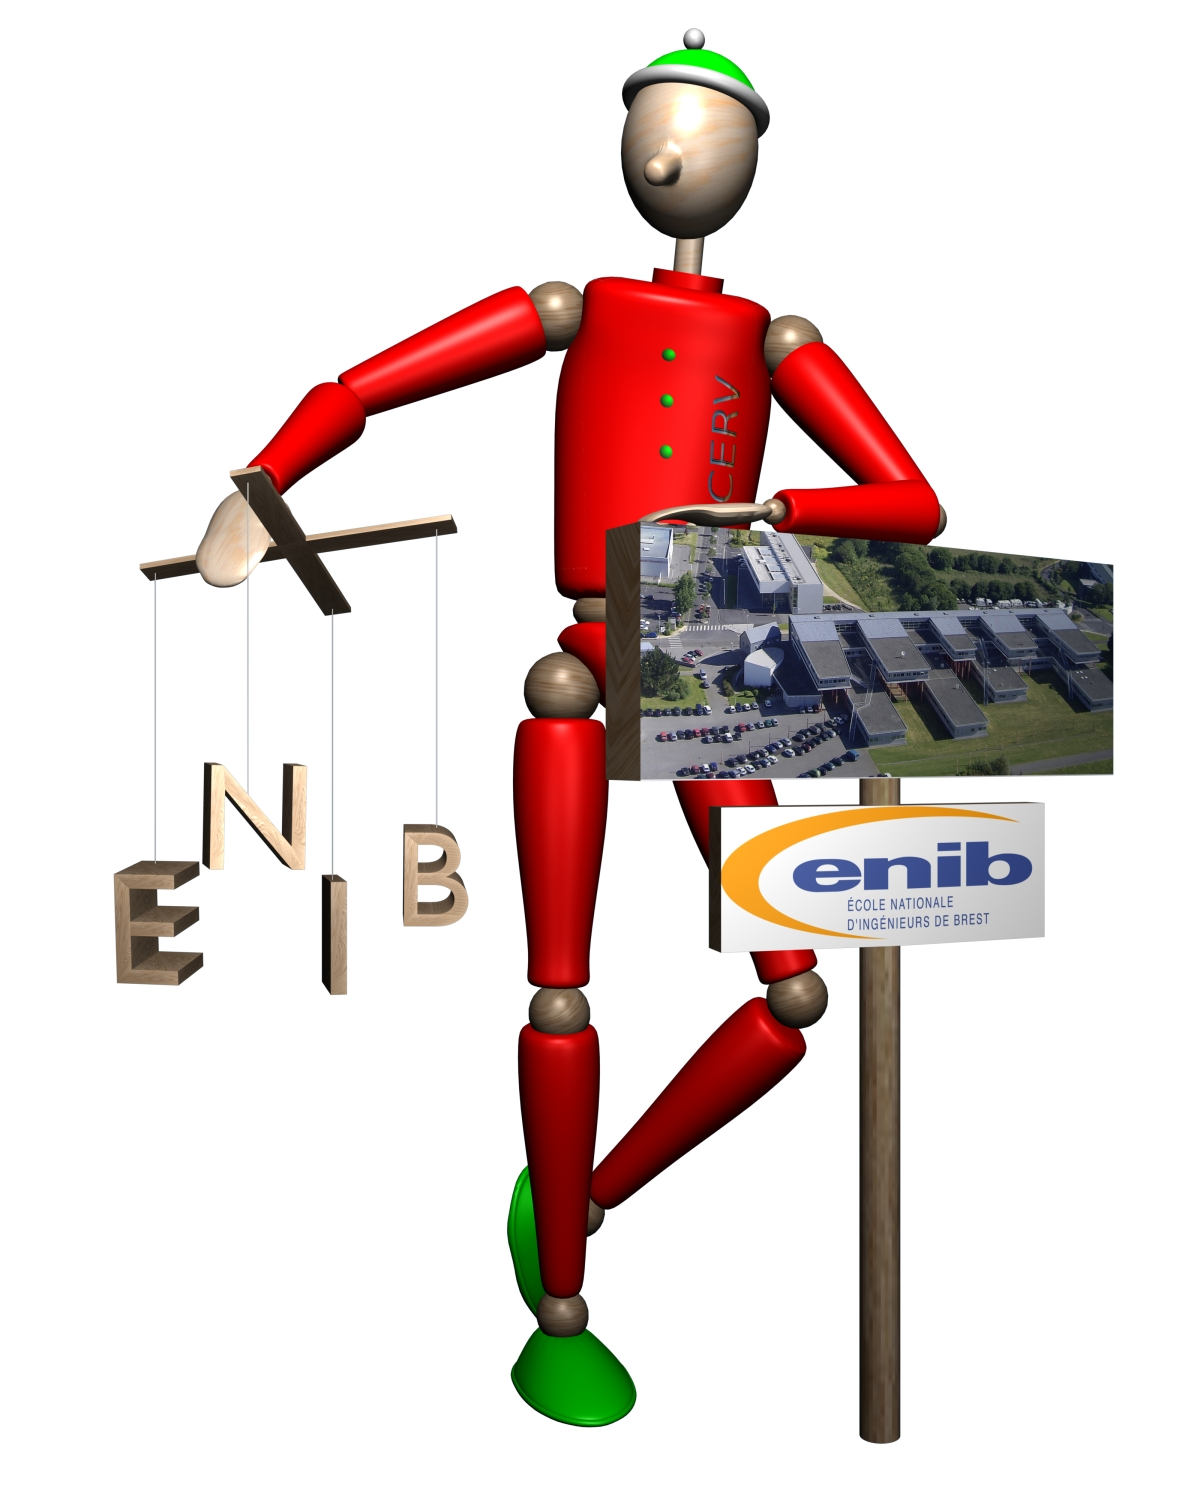
\includegraphics[width=8cm]{pinocchio-enib-small-1.jpg}}
\footnotesize\vspace*{1.5mm}
Avec la participation de {\sc Romain Bénard}, 
{\sc Stéphane Bonneaud}, {\sc Cédric Buche},
{\sc Gireg Desmeulles}, {\sc Céline Jost}, 
{\sc Sébastien Kubicki}, {\sc Eric Maisel}, 
{\sc Aléxis Nédélec}, {\sc Marc Parenthoën} et 
{\sc Cyril Septseault}.
}
\null\vfill

\noindent Ces notes de cours accompagnent les enseignements d'informatique 
du $1^{er}$ semestre (S1) de l'Ecole Nationale d'Ingénieurs 
de Brest (\enib : \href{http://www.enib.fr}{\tt www.enib.fr}). 
Leur lecture ne dispense en aucun cas
d'une présence attentive aux cours 
ni d'une participation active aux travaux dirigés.
\vspace*{0.5cm}

\centerline{\tiny version du \today}
\mbox{}

\end{titlepage}
%-------------------------------------------------------------------------

\marginpar{\renewcommand{\contentsname}{\large\bf Sommaire\vspace*{-1.5cm}}
\vspace*{-4cm}
\footnotesize\tableofcontents}
\null\vfill

	$$\begin{minipage}{12cm}\label{cite:abelson}
	« Chaque programme d'ordinateur est un modèle, forgé par l'esprit, d'un
	processus réel ou imaginaire. Ces processus, qui naissent de l'expérience et
	de la pensée de l'homme, sont innombrables et complexes dans leurs détails. 
	A tout moment, ils ne peuvent être compris que partiellement. 
	Ils ne sont que rarement modélisés d'une façon satisfaisante dans
	nos programmes informatiques. Bien que nos programmes soient des ensembles
	de symboles ciselés avec soin, des mosaïques de fonctions
	entrecroisées, ils ne cessent d'évoluer. 
	Nous les modifions au fur et à mesure que notre perception du modèle
	s'approfondit, s'étend et se généralise, jusqu'à atteindre un 
	équilibre métastable aux frontières d'une autre modélisation
	possible du problème. L'ivresse joyeuse qui accompagne la
	programmation des ordinateurs provient des allers-retours continuels,
	entre l'esprit humain et l'ordinateur, des mécanismes exprimés par
	des programmes et de l'explosion de visions nouvelles qu'ils apportent.
	Si l'art traduit nos rêves, l'ordinateur les réalise sous la forme de 
	programmes\,! »\\\mbox{}\hfill
	{\em Abelson H., Sussman G.J. et Sussman J., \cite{abelson}}
	\end{minipage}$$
\null\vfill

%-------------------------------------------------------------------------
\chapter{Introduction générale}\label{ch:introduction}
%-------------------------------------------------------------------------
	\marginpar{\vspace*{-2cm}\minitoc}
	\noindent\fbox{
\includegraphics[width=0.75\textwidth,page=1]{../../pdf/cours/introductionSlide.pdf}}
	\newpage
	% info-S1-intro.tex

%-------------------------------------------------------------------------
\section{Contexte scientifique}\label{contexte}
%-------------------------------------------------------------------------
\marginpar{\footnotesize\em
\begin{fig}[Définitions de l'Académie (1)]\label{fig:dico1}
\mbox{}\\
{\bf INFORMATIQUE} n. f. et adj. XXe siècle. Dérivé d'information sur le modèle de mathématique, électronique.
1. N. f. Science du traitement rationnel et automatique de l'information ; l'ensemble des applications de cette science. 
2. Adj. Qui se rapporte à l'informatique. Système informatique, ensemble des moyens qui permettent de conserver, 
de traiter et de transmettre l'information.

{\bf INSTRUCTION} n. f. XIVe siècle. Emprunté du latin instructio, «~action d'adapter, de ranger~», 
puis «~instruction~».
Ordre, indication qu'on donne à quelqu'un pour la conduite d'une affaire ; directive, consigne. 
Le plus souvent au pluriel. Des instructions verbales, écrites. Donner des instructions à ses collaborateurs. 
Instructions pour la mise en marche d'un appareil. Par anal. INFORM. Consigne formulée dans un langage de 
programmation, selon un code.

{\bf LOGICIEL} n. m. XXe siècle. Dérivé de logique.
INFORM. Ensemble structuré de programmes remplissant une fonction déterminée, 
permettant l'accomplissement d'une tâche donnée.

{\bf MAT\'ERIEL} adj. et n. XIIIe siècle. Emprunté du latin materialis, de même sens.
INFORM. Ensemble des éléments physiques employés pour le traitement des données, par opposition aux 
logiciels.

{\bf ORDINATEUR} n. m. XVe siècle, au sens de «~celui qui institue quelque chose~» ; XXe siècle, au sens actuel. 
Emprunté du latin ordinator, «~celui qui règle, met en ordre ; ordonnateur~».
Équipement informatique comprenant les organes nécessaires à son fonctionnement autonome, 
qui assure, en exécutant les instructions d'un ensemble structuré de programmes, 
le traitement rapide de données codées sous forme numérique qui peuvent être 
conservées et transmises.
\end{fig}} 

%-------------------------------------------------------------------------
\subsection{Informatique}
%-------------------------------------------------------------------------
Le terme {\sc informatique}\index{informatique} est un néologisme proposé en 1962 par
Philippe Dreyfus\index{{{\sc Dreyfus}}} pour caractériser le traitement automatique de l'information :
il est construit sur la contraction de l'expression  «~information automatique~».
Ce terme a été accepté par l'Académie française en avril 1966, et l'informatique devint alors
officiellement la science du traitement automatique de l'information, où l'information
est considérée comme le support des connaissances humaines et des communications 
dans les domaines techniques, économiques et sociaux (figure \ref{fig:dico1}).
Le mot {\sc informatique} n'a pas vraiment d'équivalent aux Etats-Unis où l'on parle de 
{\em Computing Science} (science du calcul) alors que {\em Informatics} est admis par les Britanniques. 

\begin{defin}[informatique]\label{def:informatique}\index[def]{informatique}
L'informatique est la science du traitement automatique de l'information.
\end{defin}

L'informatique traite de deux aspects complémentaires : les programmes immatériels (logiciel, {\em software})
qui décrivent un traitement à réaliser et les machines (matériel, {\em hardware}) 
qui exécutent ce traitement.
Le matériel est donc l'ensemble des éléments physiques (microprocesseur, mémoire, écran, clavier, disques durs\ldots)
utilisés pour traiter les données. 
Dans ce contexte, l'ordinateur\index{ordinateur} est un terme générique qui désigne un équipement informatique permettant de traiter des 
informations selon des séquences d'instructions (les programmes) qui constituent le logiciel.
Le terme {\sc ordinateur} a été proposé par le philologue Jacques Perret\index{{{\sc Perret}}} en avril 1955 
en réponse à une demande d'IBM France qui estimait le mot «~calculateur~» ({\em computer}) 
bien trop restrictif en regard des possibilités de ces machines (voir la proposition de 
Jacques Perret en annexe \ref{annexe:perret} page \pageref{annexe:perret}).

\begin{defin}[matériel]\label{def:materiel}\index[def]{matériel}\index{matériel!définition}
Le matériel informatique est un ensemble de dispositifs physiques utilisés pour traiter
automatiquement des informations.
\end{defin}
\begin{defin}[logiciel]\label{def:logiciel}\index[def]{logiciel}\index{logiciel}
Le logiciel est un ensemble structuré d'instructions décrivant un traitement d'informations
à faire réaliser par un matériel informatique.
\end{defin}

\marginpar{\footnotesize\em 
\begin{fig}[John Von Neumann\index{{{\sc Von Neumann}}} (1903-1957)]\label{fig:vonneumann}
\mbox{}\\
 \begin{minipage}{3cm}{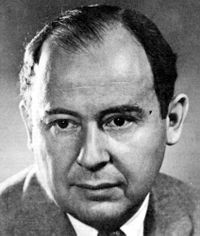
\includegraphics[width=2.5cm]{vonneumann.jpg}}
 \end{minipage}\hfill
 \begin{minipage}{4cm}
 Mathématicien américain d'ori\-gine hongroise : il a donné son nom 
 à l'architecture de von Neumann utilisée dans la quasi 
 totalité des ordinateurs modernes
 (voir figure \ref{fig:archiVN} ci-dessous).
 \end{minipage}
\end{fig}
\begin{fig}[Architecture de Von Neumann]\label{fig:archiVN}
\mbox{}\\
\centerline{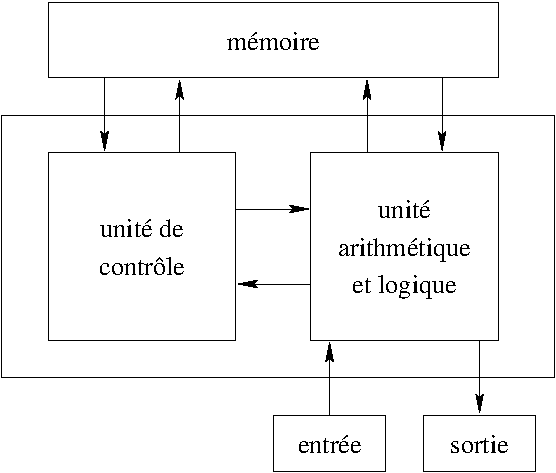
\includegraphics[width=6cm]{vonneumann.pdf}}
\end{fig}} 
Un ordinateur n'est rien d'autre qu'une machine effectuant des opéra\-tions
simples sur des séquences de signaux électriques, lesquels sont conditionnés de manière à ne pouvoir
prendre que deux états seulement (par exemple un potentiel électrique maximum ou minimum). Ces
séquences de signaux obéissent à une logique binaire du type «~tout ou rien~» et peuvent donc être
considérés conventionnellement comme des suites de nombres 
ne prenant jamais que les deux valeurs 0 et 1 : 
un ordinateur est donc incapable de traiter autre chose que des 
nom\-bres binaires.
Toute information d'un autre type doit être
convertie, ou codée, en format binaire. C'est vrai non seulement pour les données que l'on
souhaite traiter (les nombres, les textes, les images, les sons, les vidéos, etc.), mais aussi 
pour les programmes, c'est-à-dire les séquences d'instructions que l'on va fournir à la machine 
pour lui dire ce qu'elle doit faire avec ces données.


L'architecture matérielle\index{matériel!architecture de {{\sc Von Neumann}}} d'un ordinateur repose sur le modèle de Von Neumann
(figure \ref{fig:vonneumann}) qui distingue classiquement 4 parties (figure \ref{fig:archiVN}):
\begin{enumerate}
\item L'unité arithmétique et logique, ou unité de traitement, 
	effectue les opérations de base.
\item L'unité de contrôle séquence les opérations.
\item La mémoire contient à la fois les données et le programme qui dira à l'unité de contrôle 
	quels calculs faire sur ces données. La mémoire se divise entre mémoire vive volatile 
	(programmes et données en cours de fonctionnement) et mémoire de masse permanente 
	(programmes et données de base de la machine).
\item Les entrées-sorties sont des dispositifs permettant de communiquer avec le monde extérieur
	(écran, clavier, souris\ldots).
\end{enumerate}
Les 2 premières parties sont souvent rassemblées au sein d'une même structure : le micro-processeur
(la «~puce~»), unité centrale de l'ordinateur.

Dans ce cours, nous ne nous intéresserons qu'aux aspects logiciels de l'informatique.


%-------------------------------------------------------------------------
\subsection{Algorithmique}\label{subsec:algorithmique}
%-------------------------------------------------------------------------
\begin{ex}[Mode d'emploi d'un télécopieur]\label{ex:modemploi}
Extrait du mode d'emploi d'un télécopieur concernant l'envoi d'un document.
\begin{enumerate}
\item Insérez le document dans le chargeur automatique.
\item Composez le numéro de fax du destinataire à l'aide du pavé numérique.
\item Enfoncez la touche {\sc envoi} pour lancer l'émission.
\end{enumerate}
\end{ex}
\marginpar{\footnotesize\em
\begin{td}[Dessins sur la plage : exécution (1)]\label{td:plage1}
On cherche à faire dessiner une figure géométrique sur la plage 
à quelqu'un qui a les yeux bandés.

Quelle figure géométrique dessine-t-on en exécutant la suite d'instructions 
ci-dessous ?
\begin{enumerate}
\item avance de 10 pas,
\item tourne à gauche d'un angle de $120^\circ$,
\item avance de 10 pas,
\item tourne à gauche d'un angle de $120^\circ$, 
\item avance de 10 pas.
\end{enumerate}
\end{td}
}


Ce mode d'emploi précise comment envoyer un fax. Il est composé d'une suite 
ordonnée d'instructions (insérez\ldots, composez\ldots, enfoncez\ldots) qui
manipulent des données (document, chargeur automatique, numéro de fax, pavé numérique,
touche {\sc envoi}) pour réaliser la tâche désirée (envoi d'un document).
\marginpar{\footnotesize\em
\begin{fig}[Définitions de l'Académie (2)]\label{fig:dico2}
\mbox{}\\
{\bf ALGORITHME} n. m. XIIIe siècle, augorisme. Altération, sous l'influence du grec 
arithmos, «~nombre~», d'algorisme, qui, par l'espagnol, remonte à l'arabe Al-Khuwarizmi, 
surnom d'un mathématicien.
Méthode de calcul qui indique la démarche à suivre pour résoudre une série de 
problèmes équivalents en appliquant dans un ordre précis une suite finie de règles.

%{\bf DONN\'EE} n. f. XIIIe siècle, au sens de «~distribution, aumône~» ; XVIIIe siècle, 
%comme terme de mathématiques. Participe passé féminin substantivé de donner au sens de «~indiquer, dire~».
%1. Fait ou principe indiscuté, ou considéré comme tel, sur lequel se fonde un raisonnement ; 
%constatation servant de base à un examen, une recherche, une découverte. 
%{\em INFORM.} Représentation d'une information sous une forme conventionnelle adaptée à son exploitation. 
\end{fig}
}

Chacun a déjà été confronté à de tels documents pour faire fonctionner un 
appareil plus ou moins réticent et donc, consciemment ou non, 
a déjà exécuté un algorithme (ie. exécuter la suite d'instructions dans l'ordre 
annoncé, figure \ref{fig:dico2}).
\exo{td:plage1}
\begin{defin}[algorithme]\index[def]{algorithme}\index{algorithme!définition}
Un algorithme est une suite ordonnée d'instructions qui indique la démarche 
à suivre pour résoudre une série de problèmes équivalents.
\end{defin}

\begin{ex}[Trouver son chemin]\label{ex:cheminGare}
Extrait d'un dialogue entre un touriste égaré et un autochtone.
\begin{itemize}
\item Pourriez-vous m'indiquer le chemin de la gare, s'il vous plait ?
\item Oui bien sûr : vous allez tout droit jusqu'au prochain carrefour,
	vous prenez à gauche au carrefour et ensuite la troisième à droite,
	et vous verrez la gare juste en face de vous.
\item Merci.
\end{itemize}
\end{ex}

Dans ce dialogue, 
la réponse de l'autochtone est la description d'une suite ordonnée
d'instruc\-tions (allez tout droit, prenez à gauche, prenez la troisième à droite) qui
manipulent des données (carrefour, rues) pour réaliser la tâche désirée (aller à la gare).
Ici encore, chacun a déjà été confronté à ce genre de situation et donc, consciemment ou non, 
a déjà construit un algorithme dans sa tête (ie. définir la suite d'instructions pour réaliser 
une tâche).
Mais quand on définit un algorithme, celui-ci ne doit contenir que des instructions 
compréhensibles par celui qui devra l'exécuter (des humains dans les 2 exemples précédents).
\exo{td:plage2}
\marginpar{\footnotesize\em
\begin{td}[Dessins sur la plage : conception (1)]\label{td:plage2}
Faire dessiner une spirale rectangulaire de 5 côtés, le plus petit côté
faisant 2 pas de long et chaque côté fait un pas de plus que le précédent.
\end{td}
}

%\begin{shaded}
Dans ce cours, nous apprendrons à définir des algorithmes pour qu'ils soient 
compré\-hen\-si\-bles --- et donc exécutables --- par un ordinateur.
%\end{shaded}

\begin{defin}[algorithmique]\index[def]{algorithmique}\index{algorithmique}
L'algorithmique est la science des algorithmes.
\end{defin}

L'algorithmique s'intéresse à l'art de construire des algorithmes ainsi
qu'à caractériser leur validité, leur robustesse, leur réutilisabilité, 
leur complexité ou leur efficacité.

\begin{defin}[validité d'un algorithme]\index[def]{validité d'un algorithme}\index{algorithme!validité}
La validité d'un algorithme est son aptitude à réaliser exactement la tâche
pour laquelle il a été conçu.
\end{defin}
\noindent Si l'on reprend l'exemple \ref{ex:cheminGare} de l'algorithme de recherche du chemin
de la gare, l'étude de sa validité consiste à s'assurer qu'on arrive effectivement 
à la gare en exécutant scrupuleusement les instructions dans l'ordre annoncé.

\begin{defin}[robustesse d'un algorithme]\index[def]{robustesse d'un algorithme}\index{algorithme!robustesse}
La robustesse d'un algorithme est son aptitude à se protéger de conditions 
anormales d'utilisation.
\end{defin}
\noindent Dans l'exemple \ref{ex:cheminGare}, la question de la robustesse de l'algorithme
se pose par exemple si le chemin proposé a été pensé pour un piéton, alors que le 
«~touriste égaré~» est en voiture et que la «~troisième à droite~» est en sens interdit.

\marginpar{\footnotesize\em
\begin{td}[Propriétés d'un algorithme]\label{td:propPlage}
Reprendre le TD \ref{td:plage1} et illustrer la validité, la robustesse, la réutilisabilité, la
complexité et l'efficacité de l'algorithme proposé pour dessiner sur la plage.
\end{td}
\begin{fig}[Du problème au code source]\label{fig:pb2source}
\mbox{}\\
\centerline{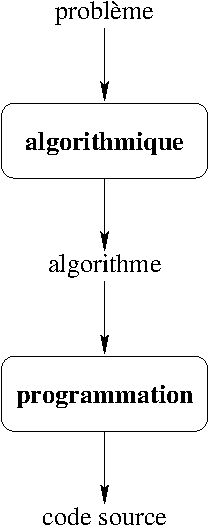
\includegraphics[width=2.5cm]{informatique.pdf}}
\end{fig}
}

\begin{defin}[réutilisabilité d'un algorithme]\index[def]{réutilisabilité d'un algorithme}\index{algorithme!réutilisabilité}
\label{definition:réutilisabilité}
La réutilisabilité d'un algorithme est son aptitude à être réutilisé pour résoudre
des tâches équivalentes à celle pour laquelle il a été conçu.
\end{defin}
\noindent L'algorithme de recherche du chemin de la gare est-il réutilisable tel quel pour se rendre
à la mairie ? A priori non, sauf si la mairie est juste à côté de la gare.

\begin{defin}[complexité d'un algorithme]\index[def]{complexité d'un algorithme}\index{algorithme!complexité}
La complexité d'un algorithme est le nombre d'instructions élémentaires à exécuter pour
réaliser la tâche pour laquelle il a été conçu.
\end{defin}
\noindent Si le «~touriste égaré~» est un piéton, la complexité de l'algorithme de recherche de chemin
peut se compter en nombre de pas pour arriver à la gare.

\begin{defin}[efficacité d'un algorithme]\index[def]{efficacité d'un algorithme}\index{algorithme!efficacité}
L'efficacité d'un algorithme est son aptitude à utiliser de manière optimale
les ressources du matériel qui l'exécute.
\end{defin}
\noindent N'existerait-il pas un raccourci piétonnier pour arriver plus vite à la gare ?
\exo{td:propPlage}

L'algorithmique permet ainsi de passer d'un problème à résoudre à un algorithme
qui décrit la démarche de résolution du problème. La programmation a alors pour rôle de traduire cet
algorithme dans un langage «~compréhensible~» par l'ordinateur afin qu'il
puisse exécuter l'algorithme automatiquement (figure \ref{fig:pb2source}).


%-------------------------------------------------------------------------
\subsection{Programmation}
%-------------------------------------------------------------------------
Un algorithme exprime la structure logique d'un programme
informatique et de ce fait est indépendant du langage de programmation 
utilisé. 
Par contre, la traduction de l'algorithme dans un langage particulier
dépend du langage choisi et sa mise en \oe uvre dépend également
de la plateforme d'exécution. 
\marginpar{\footnotesize\em
\begin{fig}[Définitions de l'Académie (3)]\label{fig:langage}
\mbox{}\\
{\bf LANGAGE}. n. m. XIIe siècle. Dérivé de langue. Système de signes, de symboles, 
élaboré à partir des langues naturelles et 
constituant un code qui les remplace dans certains cas déterminés 
(on parle aussi de langage symbolique).
%Le langage chiffré, secret, conventionnel. 
Le langage mathématique. 
Langage logique, fondé sur la logique formelle. Langage informatique. 
Langage de programmation.

{\bf BIT} n. m. XXe siècle. Mot anglo-américain, contraction de binary digit, 
«~chiffre binaire~». Chacun des deux chiffres, 0 et 1, de la numération binaire. 
En informatique, le bit est l'unité élémentaire d'information appelée aussi élément binaire.

{\bf OCTET} n. m. XXe siècle. Dérivé savant du latin octo, «~huit~».
Unité d'information composée de huit bits.
\end{fig}}

La programmation\index{programmation} d'un ordinateur consiste à lui «~expliquer~» en détail 
ce qu'il doit faire, en sachant qu'il ne «~comprend~» pas le langage humain, 
mais qu'il peut seulement effectuer un traitement 
automatique sur des séquences de 0 et de 1.
\marginpar{\footnotesize\em
\begin{fig}[Clé USB ({Universal Serial Bus})]\label{fig:cleUSB}
\mbox{}\\
\begin{minipage}{3.5cm}
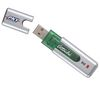
\includegraphics{usb.jpg}
\end{minipage}\hfill
\begin{minipage}{3.5cm}
Dispositif matériel 
con\-te\-nant une mé\-moi\-re de mas\-se 
(une mémoire flash ou un mini disque dur).
\end{minipage}
\end{fig}
}
Un programme n'est rien d'autre qu'une suite d'instructions, encodées en 
respectant de manière très stricte un ensemble de conventions fixées à 
l'avance par un langage informatique (figure \ref{fig:langage}). 
La machine décode alors
ces instructions en associant à chaque «~mot~»
du langage informatique une action précise.
Le programme que nous écrivons dans le langage informatique
à l'aide d'un éditeur (une sorte de traitement de
texte spécialisé) est appelé programme source (ou code source). 

Le seul «~langage~» 
que l'ordinateur puisse véritablement «~comprendre~» 
est donc très éloigné de ce que nous utilisons nous-mêmes. 
C'est une 
longue suite de 0 et de 1 (les «~bits~», {\em binary digit})\index{bit} traités par
groupes de 8 (les «~octets~», {\em byte})\index{octet}, 16, 32, ou même 64
(figure \ref{fig:langage}). 

\begin{defin}[bit, octet]\index[def]{bit}\index[def]{octet}
Un bit est un chiffre binaire (0 ou 1). 
C'est l'unité élémentaire d'information.\\
Un octet est une unité d'information composée de 8 bits.
\end{defin}

\begin{ex}[Description de clé USB]\label{ex:megaoctet}
Sur le descriptif commercial d'une clé USB (figure \ref{fig:cleUSB}), on peut lire :
\begin{itemize}
\item Type de produit  : Lecteur flash USB
\item Taille du module : 512 Mo
\item Type d'interface : Hi-Speed USB
\end{itemize}
\end{ex}
\noindent La «~taille du module~» est la capacité de stockage de la clé qui vaut ici 512 Mo (mégaoctets).
Le préfixe «~méga~» est un multiplicateur décimal qui vaut $10^6$ mais s'il est bien adapté au calcul décimal,
il l'est moins au calcul binaire car il ne correspond pas à une puissance entière de 2. 
En effet, la puissance $x$ de 2 telle que $2^x = 10^6$
vaut $\displaystyle x = 6\cdot\frac{\log(10)}{\log(2)} \approx 19.93$. On choisit alors la puissance entière de 2
immédiatement supérieure ($2^{20} = 1\,048\,576$) pour définir le Mo : 
1 Mo = 1\,048\,576 octets.
\exo{td:octets}
\marginpar{\footnotesize\em 
\begin{td}[Unités d'information]\label{td:octets}\index[td]{unités d'information}
Combien y a-t-il d'octets dans 1 ko (kilooctet), 
1 Go (gigaoctet), 1 To (téraoctet), 1 Po (pétaoctet), 1 Eo (exaoctet),
1 Zo (zettaoctet) et 1 Yo (yottaoctet) ?
\end{td}
\begin{fig}[Du code source à son exécution]\label{fig:code2exec}
\mbox{}\\
\centerline{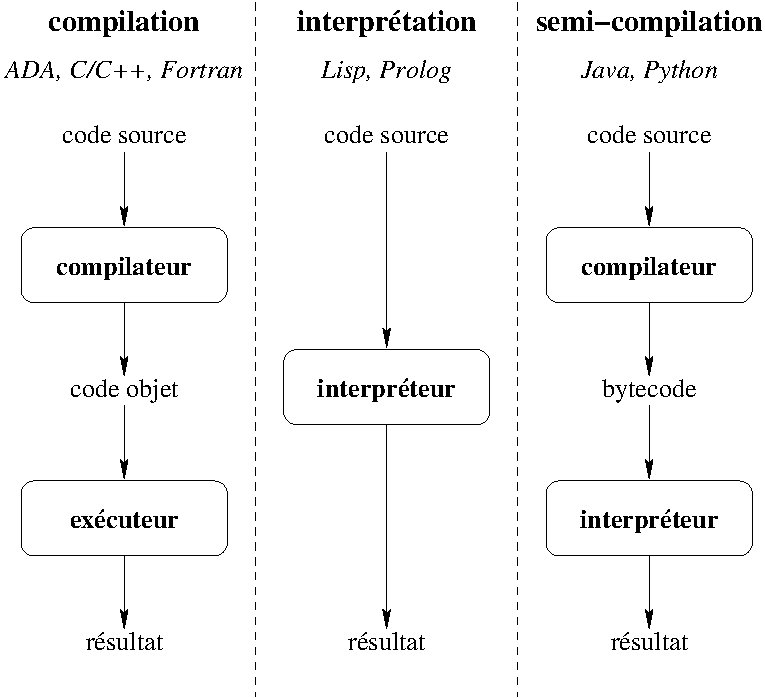
\includegraphics[width=7.5cm]{compilateur.pdf}}
\end{fig}}

Pour «~parler~» à un ordinateur, il nous faudra donc utiliser des
systèmes de traduction automatiques, capables de convertir en nombres binaires des suites de
caractères formant des mots-clés (anglais en général) qui seront plus significatifs pour nous.
Le système de traduction proprement dit s'appellera interpréteur ou bien compilateur, suivant la
méthode utilisée pour effectuer la traduction (figure \ref{fig:code2exec}). 

\begin{defin}[compilateur]\index[def]{compilateur}\index{compilateur}
	Un compilateur est un programme informatique qui traduit un langage, 
	le langage source, en un autre, appelé le langage cible. 
\end{defin}

\begin{defin}[interpréteur]\index[def]{interpréteur}\index{interpréteur}
	Un interpréteur est un outil informatique (logiciel ou matériel) ayant pour tâche 
	d'analyser et d'exécuter un programme écrit dans un langage source.
\end{defin}

On appellera langage de programmation un ensemble de mots-clés (choisis arbitrairement) 
associé à un ensemble de règles très précises indiquant comment on peut assembler ces mots 
pour former des «~phrases~» que l'interpréteur ou le compilateur puisse traduire en langage 
machine (binaire).
Un langage de programmation se distingue du langage mathématique par sa visée opérationnelle
(ie. il doit être exécutable par une machine), de sorte qu'un langage de programmation est 
toujours un compromis entre sa puissance d'expression et sa possibilité d'exécution.

\begin{defin}[langage de programmation]\index[def]{langage de programmation}\index{langage de programmation}
Un langage de programmation est un langage informatique, permettant à un 
humain d'écrire un code source qui sera analysé par un ordinateur. 
\end{defin}

Le code source subit ensuite une transformation ou une évaluation dans une forme exploitable par la machine, ce qui permet d'obtenir un programme. Les langages permettent souvent de faire abstraction des mécanismes bas niveaux de la machine, de sorte que le code source représentant une solution puisse être rédigé et compris par un humain.

\begin{defin}[programmation]\index[def]{programmation}
La programmation est l'activité de rédaction du code source d'un programme.
\end{defin}


\begin{description}
\item[Compilation :] \index{programmation!compilation} La compilation consiste à traduire la totalité du code source en une fois. 
Le compilateur lit toutes les lignes du programme source et produit une nouvelle 
suite de codes appelé programme objet (ou code objet). 
Celui-ci peut désormais être exécuté indépendamment du
compilateur et être conservé tel quel dans un fichier («~fichier exécu\-table~»).
Les langages {\sc Ada}, {\sc C}, {\sc C++} et {\sc Fortran} sont des exemples de langages 
compilés.

\item[Interprétation :] \index{programmation!interprétation} L'interprétation consiste à traduire chaque ligne du programme source en quelques instructions
du langage machine, qui sont ensuite directement exécutées au fur et à mesure
(«~au fil de l'eau~»). Aucun programme objet n'est généré.
L'interpréteur doit être utilisé chaque fois que l'on veut faire fonctionner le programme. 
Les langages {\sc Lisp} et {\sc Prolog} sont des exemples de langages interprétés.

L'interprétation est idéale lorsque l'on est en phase d'apprentissage du langage, ou en cours
d'expérimentation sur un projet. Avec cette technique, on peut en effet tester immédiatement toute
modification apportée au programme source, sans passer par une phase de compilation qui demande
toujours du temps.
Mais lorsqu'un projet comporte des fonctionnalités complexes qui doivent s'exécuter
rapidement, la compilation est préférable : un programme compilé fonctionnera
toujours plus vite que son homologue interprété, puisque dans cette technique l'ordinateur
n'a plus à (re)traduire chaque instruction en code binaire avant qu'elle puisse être exécutée.

\item[Semi-compilation :] \index{programmation!semi-compilation} Certains langages tentent de combiner les deux techniques afin de retirer le meilleur de
chacune. C'est le cas des langages {\sc Python} et {\sc Java} par exemple. 
De tels langages
commencent par compiler le code source pour produire un code intermédiaire, similaire à un langage
machine (mais pour une machine virtuelle), que l'on appelle bytecode, lequel sera ensuite transmis 
à un interpréteur pour l'exécution
finale. Du point de vue de l'ordinateur, le bytecode est très facile à interpréter en langage machine.
Cette interprétation sera donc beaucoup plus rapide que celle d'un code source.

Le fait de disposer en permanence d'un interpréteur permet de tester immédiatement n'importe
quel petit morceau de programme. On pourra donc vérifier le bon fonctionnement de chaque
composant d'une application au fur et à mesure de sa construction.
L'interprétation du bytecode compilé n'est pas aussi rapide que celle d'un véritable code machine,
mais elle est satisfaisante pour de très nombreux programmes.
\end{description}

%\begin{shaded}
Dans ce cours, nous choisirons d'exprimer directement les algorithmes dans un 
langage informatique opérationnel : le langage {\sc Python} \cite{swinnen}\label{cite:swinnen}, sans passer par un
langage algorithmique intermédiaire.
%\end{shaded}

\marginpar{\footnotesize\em
\mbox{}\hfill
\begin{minipage}{4cm}
\includegraphics[width=4cm]{python-logo.jpg}\end{minipage}
\hfill\href{http://www.python.org}{\tt www.python.org}
\hfill\mbox{}
}

%-------------------------------------------------------------------------
\section{Objectifs du cours}
%-------------------------------------------------------------------------
%La pédagogie désigne les méthodes et pratiques d'enseignement et 
%d'éducation ainsi que toutes les qualités requises pour transmettre 
%un savoir quelconque.
%
%La didactique se différencie de la pédagogie par le rôle central des contenus 
%disciplinaires et par sa dimension épistémologique (la nature des connaissances à enseigner).
%
%L'apprentissage est l'acquisition de nouveaux savoirs ou savoir-faire, 
%c'est-à-dire le processus d'acquisition de connaissances, compétences, 
%attitudes ou valeurs, par l'étude, l'expérience ou l'enseignement.


%-------------------------------------------------------------------------
\subsection{Objectifs thématiques}
%-------------------------------------------------------------------------
L'objectif principal des enseignements d'informatique S1 de l'ENIB
est l'acquisition des notions fondamentales de l'algorithmique.
\marginpar{\footnotesize\em
\begin{td}[Première utilisation de {\sc Python}]\label{td:python}\index[td]{{{\sc Python}}}
Se connecter sur un poste de travail d'une salle informatique.
\begin{enumerate}
\item Lancer {\sc Python}.
\item Utiliser {\sc Python} comme une simple calculette.
\item Quitter {\sc Python}.
\end{enumerate}
Ne pas oublier de se déconnecter du poste de travail.
\end{td}
}
Plus précisément, nous étudierons successivement :
\begin{enumerate}
\item les instructions de base permettant de décrire les algorithmes : affectation, tests, boucles;
\item les procédures et les fonctions qui permettent de structurer et de réutiliser les algorithmes;
	on parlera alors d'encapsulation, de préconditions, de portée des variables, de passage de paramètres,
	d'appels de fonctions, de récursivité et de jeux de tests;
\item les structures de données linéaires : tableaux, listes, piles, files, qui améliorent la
	structuration des données manipulées par les algorithmes. A cette occasion, on évaluera
	la complexité et l'efficacité de certains algorithmes utilisant ces structures linéaires.
\end{enumerate}
Ces différentes notions seront mise en \oe uvre à travers l'utilisation du 
langage {\sc Python}.
\exo{td:python}

%-------------------------------------------------------------------------
\subsection{Objectifs pédagogiques}\label{sub:pedago}
%-------------------------------------------------------------------------
\mbox{}
\marginpar{\footnotesize\em
\begin{fig}[Taxonomie de Bloom]\label{fig:bloom}
\mbox{}\\
Benjamin Bloom (1913-1999),
psychologue amé\-ri\-cain spécialisé en pédagogie.\\
\mbox{}\\
\centerline{\begin{tabular}{l@{ : }p{5.5cm}}
Connaître   & définir, distinguer, acquérir, identifier, rappeler, reconnaître\ldots \\
Comprendre  & traduire, illustrer, représenter, dire avec ses mots, distinguer, réécrire, 
		réarranger, expliquer, démontrer\ldots \\
Appliquer   & appliquer, généraliser, relier, choisir, développer, utiliser, employer, 
		transférer, classer, restructurer\ldots \\
Analyser    & distinguer, détecter, classer, reconnaître, catégoriser, déduire, discerner, comparer\ldots \\
Synthétiser & écrire, relater, produire, constituer, transmettre, modifier, créer, 
		proposer, planifier, projeter, spécifier, combiner, classer, formuler\ldots \\
Evaluer     & juger, argumenter, valider, décider, comparer\ldots \\
\end{tabular}}
\end{fig}}
Au cours du semestre S1, nous nous positionnerons principalement sur les 3 premiers 
niveaux de la taxonomie de Bloom\index{pédagogie!taxonomie de {{\sc Bloom}}}\index{{{\sc Bloom}}} qui constitue une référence pédagogique pour la 
classification des 
niveaux d'apprentissage (figure \ref{fig:bloom}) : connaissance, compréhension, application. 
Les 3 derniers niveaux seront plutôt abordés au cours 
du semestre S2 (analyse, synthèse, évaluation).
\begin{enumerate}
\item Connaissance : mémorisation et restitution d'informations dans les mêmes termes.
\item Compréhension : restitution du sens des informations dans d'autres termes.
\item Application : utilisation de règles, principes ou algorithmes pour résoudre un problème, les règles 
	n'étant pas fournies dans l'énoncé.
\item Analyse : identification des parties constituantes d'un tout pour en distinguer les idées.
\item Synthèse : réunion ou combinaison des parties pour former un tout.
\item Evaluation : formulation de jugements qualitatifs ou quantitatifs.
\end{enumerate}

Afin de mieux nous situer par rapport aux différents types de pédagogie
associés, nous «~filerons~» une métaphore musicale inspirée de \cite{charles}\label{cite:charles}.
\begin{description}
\item[Pédagogie par objectifs :] \index{pédagogie!pédagogie par objectifs} Le solfège est l'étude des principes élémentaires
	de la musique et de sa notation : le musicien «~fait ses gammes~» et chaque exercice
	a un objectif précis pour évaluer l'apprentissage du «~langage musical~».
	Il en va de même pour l'informaticien débutant confronté à l'apprentissage d'un 
	langage algorithmique.
\item[Pédagogie par l'exemple :] \index{pédagogie!pédagogie par l'exemple} L'apprentissage des grands classiques 
	permet au musicien
	de s'ap\-pro\-prier les bases du solfège en les appliquant à ces partitions connues et en les
	(re)jouant lui-même. L'informaticien débutant, en (re)codant lui-même des algorithmes bien
	connus, se constituera ainsi une base de réflexes de programmation en «~imitant~» ces
	algorithmes.
\item[Pédagogie de l'erreur :] \index{pédagogie!pédagogie de l'erreur} Les bogues ({\em bugs}) sont à l'informaticien ce que les fausses notes
	sont aux musiciens : des erreurs. 
	Ces erreurs sont nécessaires dans l'acquisition de la connaissance.
	Un élève a progressé si, après s'être trompé,
	il peut reconnaître qu'il s'est trompé,  dire où et pourquoi il s'est trompé,
	et comment il recommencerait sans produire les mêmes erreurs.
	\marginpar{\footnotesize\em
	\begin{rem}
	L'annexe \ref{ch:classiques} page \pageref{ch:classiques} présente quel\-ques grands classiques
	« historiques ».
	On trouvera également une liste d'algorithmes classiques sur le site 
	du National Institute of Standards and Technology {\em (\nist : \href{http://www.nist.gov/dads}{\tt
	www.nist.gov/dads})}.
	\end{rem}}
\item[Pédagogie par problèmes :] \index{pédagogie!pédagogie par problèmes} Connaissant «~ses~» classiques et les bases du solfège, le musicien
	devenu plus autonome peut envisager sereinement la création de ses propres morceaux.
	Le développement d'un projet informatique ambitieux sera «~mis en musique~» au semestre S2.
\end{description}

Dans ce cours, nous adopterons ces différentes stratégies pédagogiques sans oublier
qu'en informatique on apprend toujours mieux en faisant par soi-même.

%-------------------------------------------------------------------------
\subsection{Objectifs comportementaux}
%-------------------------------------------------------------------------
Nous cherchons à développer trois «~qualités~» comportementales chez l'informaticien
débu\-tant : la rigueur, la persévérance et l'autonomie\index{pédagogie!objectifs comportementaux}.
\begin{description}
\item[Rigueur :] Un ordinateur est une machine qui exécute vite et bien les
	instructions qu'on lui a «~apprises~». Mais elle ne sait pas interpréter
	autre chose : même mineure, une erreur provoque le dysfonctionnement de la 
	machine.
	\marginpar{\footnotesize\em
	\begin{td}[Erreur de syntaxe en {\sc Python}]\label{td:erreur}\index[td]{{{\sc Python}}}
	On considère la session {\sc Python} suivante :\\[1mm]
	\mbox{}\hfill\begin{minipage}{7cm}\tt
	>>> x = 3\\
        >>> \ y = x\\
        \mbox{}\ \ File "<stdin>", line 1\\
        \mbox{}\ \ \ \ y = x\\
        \mbox{}\ \ \ \ \char`^\\
        SyntaxError: invalid syntax\\
        >>>
	\end{minipage}\\[1mm]
	De quelle erreur de syntaxe s'agit-il ?
	\end{td}
	
	\begin{td}[Dessins sur la plage : persévérance]\label{td:plage5}\index[td]{dessins sur la plage}
	Finir l'algorithme suivant qui cherche à dessiner un losange sur la plage.
	\begin{enumerate}
	\item avance de 10 pas,
	\item tourne à gauche d'un angle de $60^\circ$,
	\end{enumerate}
	\hspace*{0.9cm}\vdots
	\end{td}
	
	\begin{td}[Autonomie]\label{td:autonomie}\index[td]{autonomie}
	Trouver les définitions du mot autonomie et de son contraire (de son antonyme).
	\end{td}
	}
	\begin{ex}[Erreur de syntaxe en langage {\sc C}]
	Pour un «~{\tt ;}~» oublié dans un programme {\sc C}, le code source n'est pas compilable
	et le compilateur nous avertit par ce type de message :\\
	
	\noindent\mbox{}\hspace*{1cm}\begin{minipage}[t]{12cm}\tt
	fichier.c: In function `main':\\
	fichier.c:7: error: syntax error before "printf"
	\end{minipage}
	\end{ex}
	Même si un humain peut transiger sur le «~{\tt ;}~», la machine ne le peut pas : 
	l'ordinateur ne se contente pas de l'«~à peu près~».
	La respect des consignes, la précision et l'exactitude sont donc de 
	rigueur en informatique !
	\exo{td:erreur}
	
\item[Persévérance :] \mbox{}
	Face à l'intransigeance de la machine, le débutant est confronté
	à ses nombreuses erreurs (les siennes, pas celles de la machine !) et sa tendance
	naturelle est de passer à autre chose. 
	Mais le papillonnage (ou {\em zapping})
	est une très mauvaise stratégie en informatique : pour s'exécuter correctement,
	un programme doit être finalisé. L'informatique nécessite d'«~aller au bout des
	choses~».
	\exo{td:plage5}
\item[Autonomie :] Programmer soi-même les algorithmes
	qu'on a définis est sans doute le meilleur moyen pour mieux assimiler
	les principales structures algorithmiques et pour mieux comprendre ses
	erreurs en se confrontant à l'intransigeante impartialité de l'ordinateur,
	vérita\-ble «~juge de paix~» des informaticiens.
	Par ailleurs, l'évolution continuelle et soutenue des langages de programmation et des 
	ordinateurs nécessitent de se tenir à jour régulièrement et seule l'autoformation systématique 
	permet de «~ne pas perdre pied~».
	\exo{td:autonomie}
	
	Pratique personnelle et autoformation constituent ainsi deux piliers de
	l'autonomisation nécessaire de l'apprenti informaticien.
\end{description}


%-------------------------------------------------------------------------
\section{Organisation du cours}
%-------------------------------------------------------------------------

%-------------------------------------------------------------------------
\subsection{Présentiel}
%-------------------------------------------------------------------------
Les enseignements d'informatique S1 de l'ENIB sont dispensés lors de 42h
de séances de cours-TD (21h) et de séances de laboratoire (21h).
\marginpar{\footnotesize\em \begin{rem} Un semestre s'étale sur 14 semaines d'enseignements. \end{rem}}
\begin{itemize}
\item Les cours-TD ont lieu chaque semaine à raison de 1h30 par semaine, soit
21h de cours-TD sur toute la durée du semestre. Ils se déroulent dans une salle
banalisée.
\item Les séances de laboratoire ont lieu 1 semaine sur 2 
à raison de 3h par semaine, soit 21h de laboratoire dans le semestre. Elles
se déroulent en salle informatique sous \linux.
\end{itemize}

\marginpar{\footnotesize\em 
\begin{fig}[Transparent de cours]\label{fig:transparent}
\mbox{}\\
\centerline{
\fbox{
\includegraphics[width=7cm,page=5]{../../pdf/cours/introductionSlide.pdf}}
}
\end{fig}
\begin{td}[Site {\sc Web} d'Informatique S1]\label{td:site}\index[td]{site {{\sc Web}}}
Se connecter sur le \href{https://moodle.enib.fr/course/view.php?id=24}{site {\sc Web} du cours d'Informatique S1} de l'\enib{} et
vérifier que ces notes de cours y sont bien disponibles au format {\tt pdf}.
\end{td}
}

%-------------------------------------------------------------------------
\subsection{Documents}
%-------------------------------------------------------------------------
Les principaux documents accompagnant les cours sont de 2 types : 
les supports de cours et les notes de cours.
\begin{description}
\item[Support de cours :] \mbox{}
	il s'agit de la copie papier des transparents projetés
	en présentiel (figu\-re~\ref{fig:transparent}). 
\item[Notes de cours :] il s'agit de notes qui complètent et
	précisent certains points présentés en cours. Ces notes proposent
	également les exercices de travaux dirigés qui sont étudiés
	en cours et au laboratoire. Le document que vous 
	êtes en train de lire constitue le premier chapitre des notes du cours
	d'informatique S1 de l'ENIB. Il y en aura 3 autres 
	sur les sujets suivants :
	\begin{enumerate}
	\item les instructions de base (chapitre \ref{ch:instructions} page \pageref{ch:instructions}),
	\item les procédures et les fonctions (chapitre \ref{ch:fonctions} page \pageref{ch:fonctions}),
	\item les structures de données linéaires (chapitre \ref{ch:listes} page \pageref{ch:listes}).
	\end{enumerate}
\end{description}

Un \href{https://moodle.enib.fr/course/view.php?id=24}{site {\sc Web} du cours d'Informatique S1} permet de retrouver ces documents au format {\tt pdf} 
({\em Portable Document Format}) ainsi que d'autres documents tels que
le planning prévisionnel des cours et des contrôles, des exemples corrigés 
d'évaluation, les notes aux différents contrôles ou encore des liens vers 
des sites pertinents pour le cours. 
\exo{td:site}

La consultation régulière du 
\href{https://moodle.enib.fr/course/view.php?id=24}{site {\sc Web} du cours d'Informatique S1} 
est indispensable pour se tenir au courant des dernières évolutions du cours : en cas d'ambiguïté,
ce sont les informations de ce site qui feront foi.


%-------------------------------------------------------------------------
\subsection{Evaluations des apprentissages}\label{sub:evaluation}
%-------------------------------------------------------------------------
L'évaluation des connaissances et des compétences acquises par les étudiants
repose sur 4 types de contrôle\index{contrôle|see{évaluation}} : les contrôles d'attention, les contrôles de \tdir, 
les contrôles d'autoformation et les contrôles de compétences.
\begin{description}
\item[Contrôle d'attention :] \mbox{}\index{evaluation@évaluation!contrôle d'attention}\index{evaluation@évaluation!qcm|see{contrôle d'attention}}\marginpar{\footnotesize\em 
\begin{td}[Exemple de contrôle d'attention (1)]\label{td:attention1}\index[td]{contrôle d'attention}
Répondre de mémoire aux questions suivantes (ie. sans rechercher les 
solutions dans les pages précédentes).
\begin{enumerate}
\item Quels sont les 3 principaux thèmes informatiques abordés ?
\item Quelles sont les 4 principales stratégies péda\-go\-giques suivies ?
\item Quelles sont les 3 principales qualités comportementales recherchées ?
\end{enumerate}
\end{td}}
	il s'agit d'un \qcm\ (questionnaire à choix multiples) 
	auquel il faut répondre individuellement
	sans document, en 5' en fin de séance, et dont les questions portent 
	sur des points abordés pendant la séance. Ce type de contrôle teste directement
	l'acquisition de connaissances au sens du «~connaître~» de la classification de
	Bloom (section~\ref{sub:pedago} page \pageref{sub:pedago}).
	Il permet d'évaluer «~à chaud~» la capacité d'attention des étudiants et les incite 
	à une présence attentive afin de bénéficier au maximum des heures de présence 
	aux cours. 	
	\exo{td:attention1}
	
	Des exemples de \qcm\ sont systématiquement proposés dans les notes de cours
	comme par exemple celui du \tdir\ \ref{td:qcmIntro} page
	\pageref{td:qcmIntro} pour cette introduction générale.
\item[Contrôle de \tdir\ :]\mbox{}\index{evaluation@évaluation!contrôle de TD} 
	il s'agit ici d'inciter les étudiants à préparer
	activement les séances de laboratoire. 
	\marginpar{\footnotesize\em 
	\begin{td}[Exemple de contrôle de TD]\label{td:TD}\index[td]{contrôle de TD}
	Répondre aux questions du TD \ref{td:attention1} situé dans la marge 
	de la page \pageref{td:attention1}.
	\end{td}
	
	\begin{td}[Exemple de contrôle d'autoformation (1)]\label{td:bool}\index[td]{contrôle d'autoformation}
	Etablir la table de vérité du circuit logique ci-dessous où $a$, $b$
	et $c$ sont les entrées, $s$ et $t$ les sorties.\\[2mm]
	\centerline{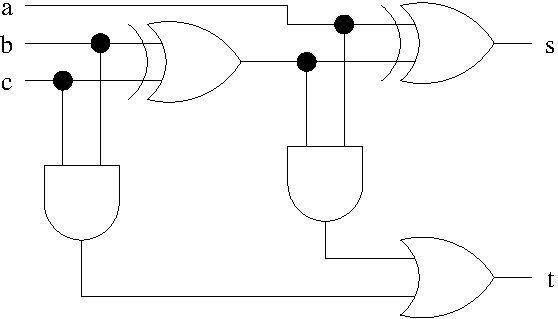
\includegraphics[width=6cm]{add3.pdf}}
	\end{td}}
	En début de chaque séance de 
	laboratoire, chaque binôme doit répondre sans document en 10' aux questions
	d'un exercice de \tdir.
	L'exercice est choisi aléatoirement parmi les exercices 
	des notes de cours et se rapportant au thème du \tdir. 
	\exo{td:TD}

	Il concerne le «~comprendre~» et l'«~appliquer~» de la taxonomie de Bloom
	(section \ref{sub:pedago} page \pageref{sub:pedago}).
\item[Contrôle d'autoformation :] \mbox{}\index{evaluation@évaluation!contrôle d'autoformation}
	un contrôle d'autoformation porte sur un thème
	prévu à l'avance et que l'étudiant doit approfondir par lui-même. Les thèmes 
	retenus pour l'autoformation en S1 sont par exemple le calcul booléen,
	le codage des nombres ou encore la recherche d'éléments dans un tableau de données.
	\exo{td:bool}

	Ces contrôles se déroulent pendant les séances de cours : 
	ce sont des écrits individuels de 30' sans document qui concernent
	le «~connaître~», le «~comprendre~» et l'«~appliquer~» de la taxonomie de Bloom.
\item[Contrôle de compétences :] \mbox{}\index{evaluation@évaluation!contrôle de compétence}\index{evaluation@évaluation!ds|see{contrôle de compétence}}
	les contrôles de compétences (ou \ds) durent 90'
	pendant ou hors d'une séance de cours. Plus longs, ils permettent d'aborder l'un des 3 
	derniers niveaux de la classification de Bloom (analyser, synthétiser, évaluer)
	comme le font les exercices de la section \ref{sub:analyser} page \pageref{sub:analyser}.
	\exo{td:competences}
\end{description}

	\marginpar{\footnotesize\em 
	\begin{td}[Exemple de contrôle des compétences]\label{td:competences}\index[td]{contrôle des compétences}
	Répondre aux questions du TD \ref{td:shadok} de la page \pageref{td:shadok}.
	\end{td}

	\begin{fig}[Métaphore de la cible]\label{fig:cible}
	\mbox{}\\
	\centerline{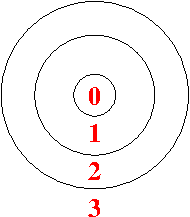
\includegraphics{cible.pdf}}
	\end{fig}
	
	\begin{rem}
	Pour obtenir une note plus « classique » (ie. une note sur 20 : $n_{/20}$), 
	il suffit de prendre le complément à 4 de la note sur 0 ($n_{/0}$) et de le 
	multiplier par 5 :
	
	$$n_{/20} = (4 - n_{/0})\times 5$$
	$$\begin{array}{r|r|l}
	n_{/0} & n_{/20} & \mbox{signification} \\
	\hline
	0 & 20 & \mbox{l'objectif est atteint}\\
	1 & 15 & \mbox{on se rapproche de l'objectif}\\
	2 & 10 & \mbox{on est encore loin de l'objectif}\\
	3 &  5 & \mbox{l'objectif n'est pas atteint}\\
	4 &  0 & \mbox{l'objectif n'a pas été visé}
	\end{array}$$
	Ainsi, dans ce contexte, avoir $20/20$ ne signifie pas qu'on est génial ou que c'est parfait,
	cela signifie « juste » qu'on a atteint un objectif fixé, et c'est déjà beaucoup !
	\end{rem}
	}

\noindent Quel que soit le type de contrôle, un exercice cherche à évaluer un objectif
particulier. Aussi, la notation\index{evaluation@évaluation!notation} exprimera la distance qui reste à parcourir 
pour atteindre cet objectif (figure \ref{fig:cible}): 
$$\begin{tabular}{l@{ : }l@{ $\rightarrow$ }l}
0 & «~en plein dans le mille !~» & l'objectif est atteint \\
1 & «~pas mal !~» & on se rapproche de l'objectif \\
2 & «~juste au bord de la cible !~» & on est encore loin de l'objectif\\
3 & «~la cible n'est pas touchée !~» & l'objectif n'est pas atteint\\
4 & «~la cible n'a pas été visée !~» & absence lors de l'évaluation
\end{tabular}$$
Ainsi, et pour changer de point de vue sur la notation, le contrôle 
est réussi lorsqu'on a 0 ! Il n'y a pas non plus de $1/2$ point ou de $1/4$ 
de point : le seul barême possible ne comporte que 4 niveaux utiles : 0, 1, 2, 3
et un cinquième pour les absences (4).
On ne cherche donc pas à «~grappiller~» des points : 
\begin{itemize}
\item on peut avoir 0 (objectif atteint) et avoir fait une ou deux erreurs 
	bénignes en regard de l'objectif recherché;
\item on peut avoir 3 (objectif non atteint) et avoir quelques éléments de
	réponse corrects mais sans grand rapport avec l'objectif.
\end{itemize}

%-------------------------------------------------------------------------
\subsection{Evaluation des enseignements}
%-------------------------------------------------------------------------
En fin de semestre, les étudiants organisent de manière anonyme et 
dans le respect des personnes, une évaluation individuelle des enseignements.
\index{evaluation@évaluation!evaluation@évaluation des enseignements}
Elle est structurée en 2 parties :
un questionnaire de 10 à 20 questions (voir un exemple en annexe
\ref{annexe:eval} page \pageref{annexe:eval}) 
auxquelles il faut répondre selon une grille pré-définie
et une partie « expression libre » que l'étudiant remplit, ou non, à son gré.

L'ensemble des fiches d'évaluation est remis à l'équipe pédagogique
d'Informatique S1, qui après en avoir pris connaissance, organise une rencontre spécifique
avec les étudiants. Cette évaluation a pour objectif l'amélioration de la qualité 
des enseignements et de la pédagogie à partir de la perception qu'en ont les étudiants.

%-------------------------------------------------------------------------
\section{Méthodes de travail}
%-------------------------------------------------------------------------
Il ne s'agit pas ici d'imposer des méthodes de travail, 
mais de fournir des pistes pour ceux qui en cherchent.
\marginpar{\footnotesize\em
\begin{rem}
Ce document comporte \pageref{LastPage} pages 
structurées en 4 chapitres, 3 annexes, 4 index et une
bibliographie. 
Il propose 
50 définitions, 
82 figures, 
39 exemples, 
76 remarques, 
128 exercices et 
5 contrôles types corrigés.
En moyenne, au cours des 14 semaines que dure le cours d'informatique S1 
de l'\enib, {\color{red}le travail personnel hebdomadaire consiste donc à
lire entre 15 et 20 pages de ce cours en retenant 3 à 4 définitions 
et en faisant entre 7 et 10 exercices.}
\end{rem}

\begin{td}[Nombre de contrôles]\label{td:controles}\index[td]{nombre de contrôles}
Après consultation du calendrier prévisionnel de l'annexe \ref{annexe:planning} 
page \pageref{annexe:planning}, donner le nombre et le type de contrôles prévus
au calendrier du semestre.
\end{td}}
Dans tous les cas, l'expérience montre que :
\begin{enumerate}
\item la seule présence, même attentive et active, aux séances de cours 
	et de laboratoire ne suffit pas : il faut prévoir un temps de travail personnel
	qui, selon l'étudiant et la matière, peut aller de 50\% à 150\% du temps de 
	présence en cours;
\item la régularité dans le travail personnel est un gage d'apprentissage
	plus efficace.
\end{enumerate}
Le calendrier prévisionnel des enseignements et des contrôles associés
est distribué en début de semestre (un exemple de planning est donné
en annexe \ref{annexe:planning} page \pageref{annexe:planning}).
\exo{td:controles} 

\noindent Les documents de cours sont tous disponibles 
sur le \href{https://moodle.enib.fr/course/view.php?id=24}{site {\sc Web} du cours d'Informatique S1}.

%-------------------------------------------------------------------------
\subsection{Avant, pendant et après le cours}\label{sub:cours}
%-------------------------------------------------------------------------
\begin{description}
\item[Préparation :] \index{pédagogie!méthodes de travail!préparation} 
	Certains cours débutent par un contrôle d'autoformation
	(voir section \ref{sub:evaluation}) dont le thème est en rapport avec certains
	aspects du cours qui a précédé ou qui suivra immédiatement.
	Il est donc nécessaire d'avoir étudié avant et par soi-même le
	sujet du contrôle.
	
	En général, on trouvera les informations nécessaires
	soit directement sur le 
	\href{https://moodle.enib.fr/course/view.php?id=24}{site {\sc Web} du cours d'Informatique S1}, 
	soit dans les références bibliographiques données en fin des notes de cours
	(voir par exemple les références de ce chapitre en page \pageref{ch:biblio}),
	soit dans les polycopiés d'autres cours de l'\enib\ (mathématiques, 
	électronique, productique, microprocesseurs\ldots), soit encore sur internet
	en s'assurant de la qualité du site (préférer des sites universitaires ou 
	d'écoles dont l'activité principale est d'enseigner ces matières).
	
	\marginpar{\footnotesize\em
	\begin{td}[Exemple de contrôle d'autoformation (2)]\label{td:negation}\index[td]{contrôle d'autoformation}
	Exprimer en la développant la négation des expressions booléennes suivantes :
	\begin{enumerate}
	\item {\tt (0 < x) and (x < 3)}
	\item {\tt (x < -2) or (x > 4)}
	\item {\tt a and (not b)}
	\item {\tt (not a) or b}
	\end{enumerate}
	\end{td}}
	Par exemple, il est nécessaire d'avoir assimilé les principes
	du calcul booléen pour maîtriser les tests et les boucles du
	langage algorithmique. C'est pourquoi, une autoformation est
	imposée sur ce domaine déjà connu des étudiants.
	Un contrôle-type d'autoformation sur le calcul booléen 
	pourrait par exemple être composé des \tdir\ \ref{td:bool} 
	page \pageref{td:bool} et \ref{td:negation} ci-contre.\\
	\exo{td:negation}
	
	Pour chaque contrôle d'autoformation, un exemple corrigé est
	disponible sur le 
	\href{https://moodle.enib.fr/course/view.php?id=24}{site {\sc Web} du cours d'Informatique S1}. 
	Il est donc fortement 
	recommandé de travailler ce contrôle-type : après avoir revu
	par soi-même les principales notions du domaine, faire
	le contrôle sans consulter au préalable la solution proposée. 
	
\item[Participation :] \index{pédagogie!méthodes de travail!participation} 
	Par respect pour les autres participants, 
	la ponctualité est de rigueur pour l'étudiant comme pour l'enseignant.
	\marginpar{\footnotesize\em
	\begin{fig}[Support de cours]\label{fig:support}
	\mbox{}\\
	\centerline{
	\fbox{\includegraphics[width=3.8cm,page=2]{../../pdf/cours/introductionPaper.pdf}}
	%\includeslide[width=3.8cm]{informatique<4>}
	}
	\end{fig}
	
	\begin{td}[Exemple de contrôle d'attention (2)]\label{td:attention2}\index[td]{contrôle d'attention}
	Répondre de mémoire aux questions suivantes (ie. sans rechercher les 
	solutions dans les pages précédentes).
	\begin{enumerate}
	\item Quels sont les 4 types de contrôle proposés ?
	\item Quels sont les documents que l'on peut trouver sur le 
		\href{https://moodle.enib.fr/course/view.php?id=24}{site {\sc Web} du cours d'Informatique S1} ?
	\end{enumerate}
	\end{td}}
	\marginpar{\footnotesize\em
	}
	Mais assister à un cours n'a d'intérêt que dans le cas d'une 
	présence attentive et soutenue : le temps passé en cours 
	pour assimiler les nouvelles notions sera gagné sur le temps de
	travail personnel futur nécessaire à leur assimilation.
	Chaque page des supports de cours est constituée
	d'une copie d'un transparent de cours dans la demi-page supérieure
	alors que la demi-page inférieure est volontairement laissée en partie vierge
	pour que l'étudiant prenne des notes pendant le cours (figure \ref{fig:support}).

	
	La prise de note systématique est en effet un facteur qui favorise l'attention et la mémorisation.
	Un contrôle de type \qcm\ en fin de cours évaluera l'attention
	des étudiants (voir section \ref{sub:evaluation}). 
	\exo{td:attention2}

	Le cours est illustré par des exemples et des exercices : à ces occasions, 
	c'est une participation active de l'étudiant qui est attendue dans une
	démarche volontaire d'assimilation du cours « à chaud ».
	
\item[Appropriation :] \index{pédagogie!méthodes de travail!appropriation} 
	Dans la mesure du possible, il faut relire ses propres notes 
	ainsi que les notes de cours le soir même afin de « fixer » les principales
	idées du cours. La révision proprement dite peut venir ultérieurement
	quelques jours plus tard (et non quelques semaines ni quelques mois après).
	
	Les définitions, comme toute définition, sont à apprendre par c\oe ur
	\label{parcoeur}.
	Une technique possible est de lire 2 fois de suite à voix haute la définition
	en détachant distinctement les différentes expressions (exemple: «~l'informatique~»
	«~est la science~» «~du traitement~» «~automatique~» «~de l'information~»),
	puis l'écrire de mémoire.
	
	Pour réviser le cours, faire systématiquement les \tdir\ au moment où ils sont
	référencés dans les notes par le symbole {\color{blue}$\rule{2mm}{2mm}\,$}
	\label{appropriation}. 
	C'est particulièrement vrai 
	avec les exemples pour lesquels sont associés des exercices en marge des
	notes de cours
	(exemple : l'exemple \ref{ex:modemploi} de la page~\pageref{ex:modemploi}
	et le \tdir\ \ref {td:plage1} associé en marge de la même page).
	Lorsque l'exemple est un algorithme, il faut  systématiquement se mettre 
	mentalement à la place de la machine qui va les exécuter (on parle alors 
	d'«~empathie numérique~») afin de vérifier le résultat obtenu. 
	Pour cela, il faut être méthodique et rigoureux. 
	Et petit à petit, à force de pratique, l'expérience fera qu'on « verra » 
	le résultat produit par les instructions au fur et à mesure qu'on les écrit. 
	Naturellement, cet apprentissage est long, et demande des heures de travail 
	patient. Aussi, dans un premier temps, il faut éviter de sauter les étapes : 
	la vérification méthodique, pas à pas, de chacun des algorithmes 
	représente plus de la moitié du travail à accomplir 
	\cite{darmengeat}\label{cite:darmengeat}.
\end{description}

%-------------------------------------------------------------------------
\subsection{Avant, pendant et après le laboratoire}
%-------------------------------------------------------------------------
\begin{description}
\item[Préparation :] \mbox{}\index{pédagogie!méthodes de travail!préparation}
	\marginpar{\footnotesize\em
	 \begin{td}[Nombres d'exercices de \tdir]\label{td:exercices}\index[td]{nombres d'exercices de \tdir}
	 Combien d'exercices y avait-il à faire avant celui-ci ?
	 \end{td}}
	Faire les exercices de ces notes de cours
	est non seulement une façon de réviser son cours (voir section \ref{sub:cours})
	mais aussi de préparer les séances de laboratoire.
	Pour ces notes de cours, la liste complète des exercices est donnée en 
	annexe \ref{ch:exercices} page \pageref{ch:exercices}.
	Un de ces exercices choisi aléatoirement fera l'objet d'une
	évaluation en début de chaque séance de \tdir\ (voir section \ref{sub:evaluation}).
	\exo{td:exercices}
	
	Tous ces exercices ne nécessitent pas une longue phase de réflexion comme
	les \tdir\ \ref{td:prop} ou \ref{td:competences} ($\rightarrow$ \ref{td:shadok}).
	Certains au contraire ne présentent aucune difficulté particulière
	comme les \tdir\ \ref{td:controles} et \ref{td:exercices}
	qui demandent simplement de compter les contrôles et les exercices.
	D'autres comme les \tdir\ \ref{td:attention1} et \ref{td:attention2} 
	font appel à la mémoire, d'autres encore à la recherche d'informations
	comme les \tdir\ \ref{td:octets} et \ref{td:autonomie}, ou à une mise en
	\oe uvre pratique comme les \tdir\ \ref{td:python} et \ref{td:site}.
\item[Participation :] \mbox{}\index{pédagogie!méthodes de travail!participation}\marginpar{\footnotesize\em
	\begin{td}[Environnement de travail]\label{td:labo}\index[td]{{{\sc Python}}}\index[td]{environnement de travail}
	Sur un poste de travail d'une salle informatique :
	\begin{enumerate}
	\item Quel est le type de clavier ?
	\item Comment ouvre-t-on un terminal ?
	\item Comment lance-t-on {\sc Python} ?
	\item Où sont stockés les fichiers de travail ?
	\end{enumerate}
	\end{td}}
	Ici encore, par respect pour les autres participants, 
	la ponctualité est de rigueur pour l'étudiant comme pour l'enseignant.

	En informatique, lorsqu'on travaille en binôme, il faut régulièrement 
	alterner les rôles entre l'«~écrivain~» qui manipule clavier et souris 
	et le «~lecteur~» qui vérifie la production de l'écrivain. A la fin
	du semestre, chaque étudiant doit être devenu un «~lecteur-écrivain~».
	La pratique est en effet nécessaire pour «~apprivoiser~» l'environnement 
	de travail afin que la machine devienne «~transparente~» et que seul 
	subsiste le problème algorithmique à résoudre.
	\exo{td:labo}
	
	Pour certains exercices, la solution est donnée dans les notes de cours
	(en section \ref{sub:solutionsIntro} page \pageref{sub:solutionsIntro} pour ce chapitre).
	Pendant les séances de laboratoire, il faut donc savoir «~jouer le jeu~»
	pour ne pas simplement «~recopier~» la solution proposée (il existe
	d'ailleurs d'autres solutions pour la plupart des exercices).
	
	Un apprenti programmeur est toujours confronté à ses propres erreurs
	(revoir le \tdir\ \ref{td:erreur} page \pageref{td:erreur} par exemple). 
	En général, ce sont des erreurs simples à corriger à condition
	de lire les messages d'erreur et de faire l'effort 
	de les comprendre avant d'appeler l'enseignant «~à l'aide~».
	\begin{ex}[Erreur de nom en {\sc Python}]
	Voici une erreur classique d'une variable non correctement initialisée en {\sc Python} :\\[1mm]
	\mbox{}\hspace*{1cm}\begin{minipage}{12cm}\tt
	>>> print(x)\\
        Traceback (most recent call last):\\
        \mbox{}\ \ File "<stdin>", line 1, in ?\\
        NameError: name 'x' is not defined\\
        >>> 
	\end{minipage}
	\end{ex}
	En {\sc Python}, la dernière ligne du message d'erreur est la plus 
	«~parlante~» au débutant.
\item[Appropriation :] \index{pédagogie!méthodes de travail!appropriation}
	Avant le cours suivant, il faut refaire les \tdir\ qui
	ont posé des problèmes et faire les exercices qui n'ont pas pu
	être abordés en séance de laboratoire (les solutions de ces
	exercices complémentaires sont données dans les notes de cours).
\end{description}	


%-------------------------------------------------------------------------
\subsection{Apprendre en faisant}
%-------------------------------------------------------------------------
	\index{pédagogie!apprendre en faisant}
	\begin{enumerate}
	\item En bas de la page \pageref{parcoeur}, il est dit :
	\begin{quote}
	« Les définitions, comme toute définition, sont à apprendre par c\oe ur. »
	\end{quote}
	Connaissez-vous les 16 définitions introduites dans ce chapitre ?
	Elles sont clairement identifiables grâce au mot-clé 
	« {\bf Définition} ».
	
	\item En haut de la page \pageref{appropriation}, il est dit :
	\begin{quote}
	« Pour réviser le cours, faire systématiquement les \tdir\ au moment où ils sont
	référencés dans les notes par le symbole {\color{blue}$\rule{2mm}{2mm}\,$}. »
	\end{quote}
	\marginpar{\footnotesize\em
	\begin{rem}
	La dernière phrase de cette section a déjà été écrite dans le texte qui précède.
	A propos de quoi ? En quelle page ?
	\end{rem}}
	Avez-vous cherché à résoudre les 18 exercices de \tdir\ proposés jusqu'à présent ?
	Ils sont clairement identifiables grâce au mot-clé « {\color{blue}\bf \tdir} » situé dans
	la marge.
	\end{enumerate}
	Il n'y a pas de miracle, c'est votre travail personnel qui est le meilleur 
	gage de vos apprentissages. On apprend toujours mieux en faisant par soi-même.

%-------------------------------------------------------------------------
\newpage
\setlength{\textwidth}{25cm}
\setlength{\textheight}{16cm}
\setlength{\marginparwidth}{0cm}
\setlength{\marginparsep}{0cm}
\setlength{\linewidth}{25cm}
\setlength{\oddsidemargin}{0cm}
\setlength{\evensidemargin}{0cm}
\setlength{\topmargin}{-0.75cm}

\section{Exercices complémentaires}
%-------------------------------------------------------------------------

%-------------------------------------------------------------------------
\subsection{Connaître}
%-------------------------------------------------------------------------
\begin{td}[QCM (1)]\label{td:qcmIntro}\index{evaluation@évaluation!contrôle d'attention}\index[td]{contrôle d'attention}
(un seul item correct par question)
\em
\begin{enumerate}
\item L'informatique est la science
%\marginpar{\footnotesize\em
%\begin{rem} Parmi les 4 items de la question ci-contre, un seul item définit
%	l'informatique, les 3 autres définissent d'autres sciences.
%	Lesquelles ?
%\end{rem}
%}
	\begin{enumerate}
	\item des dispositifs dont le fonctionnement dépend de 
		la circulation d'électrons
	\item des signaux électriques porteurs d'information ou d'énergie
	\item du traitement automatique de l'information
	\item de la commande des appareils fonctionnant sans intervention humaine
	\end{enumerate}
\item Le logiciel est
	\begin{enumerate}
	\item la mémoire de l'ordinateur
	\item le traitement automatique de l'information
	\item l'ensemble des données manipulées par les instructions
	\item un ensemble structuré d'instructions décrivant un traitement d'informations
		à faire réaliser par un matériel informatique
	\end{enumerate}
\item L'algorithmique est la science
	\begin{enumerate}
	\item du traitement automatique de l'information
	\item des algorithmes
	\item des langages de programmation
	\item des instructions
	\end{enumerate}
\item Un algorithme est
	\begin{enumerate}
	\item un ensemble de programmes remplissant une fonction déterminée,
		permettant l'accomplissement d'une tâche donnée
	\item une suite ordonnée d'instructions qui indique la démarche 
		à suivre pour résoudre une série de problèmes équivalents
	\item le nombre d'instructions élémentaires à exécuter pour
		réaliser une tâche donnée
	\item un ensemble de dispositifs physiques utilisés pour traiter
		automatiquement des informations
	\end{enumerate}
\newpage
\item La validité d'un algorithme est son aptitude
	\begin{enumerate}
	\item à utiliser de manière optimale les ressources du matériel qui l'exécute
	\item à se protéger de conditions anormales d'utilisation
%\marginpar{\footnotesize\em
%\begin{rem} Parmi les 4 items de la question précédente, un seul item définit
%	la validité d'un algorithme, les 3 autres se rapportent à d'autres propriétés
%	des algorithmes. Lesquelles ?
%\end{rem}
%}
	\item à calculer le nombre d'instructions élémentaires nécessaires pour
		réaliser la tâche pour laquelle il a été conçu
	\item à réaliser exactement la tâche pour laquelle il a été conçu
	\end{enumerate}
	\begin{rem} Parmi les 4 items de la question ci-contre, un seul item définit
	la validité d'un algorithme, les 3 autres se rapportent à d'autres propriétés
	des algorithmes. Lesquelles ?
	\end{rem}
\item La complexité d'un algorithme est
	\begin{enumerate}
	\item le nombre de fois où l'algorithme est utilisé dans un programme
	\item le nombre de données manipulées par les instructions de
		l'algorithme
	\item le nombre d'octets occupés en mémoire par l'algorithme
	\item le nombre d'instructions élémentaires à exécuter pour
		réaliser la tâche pour laquelle il a été conçu
	\end{enumerate}
\item Un bit est 
	\begin{enumerate}
	\item un chiffre binaire
	\item composé de 8 chiffres binaires
	\item un chiffre héxadécimal
	\item un mot d'un langage informatique
	\end{enumerate}
\item Un compilateur 
	\begin{enumerate}
	\item exécute le code source
	\item exécute le bytecode
	\item traduit un code source en code objet
	\item exécute le code objet
	\end{enumerate}
\end{enumerate}
\end{td}

\begin{td}[Puissance de calcul]\label{td:mips}\index{matériel!mips}\index[td]{puissance de calcul}
\em
Donner l'ordre de grandeur en instructions par seconde des machines suivantes 
(voir \cite{delahaye} par exemple) :
\begin{enumerate}
\item le premier micro-ordinateur de type PC,
\item une console de jeu actuelle,
\item un micro-ordinateur actuel,
\item {\em Deeper-Blue} : l'ordinateur qui a « battu » Kasparov aux échecs en 1997.
%\item le plus puissant ordinateur actuel.
\end{enumerate}
\end{td}

\begin{td}[Stockage de données]\label{td:stock}\index[td]{stockage de données}
\em
Donner l'ordre de grandeur en octets pour stocker en mémoire
(voir \tdir\ \ref{td:octets} et \cite{delahaye} par exemple) :
\begin{enumerate}
\item une page d'un livre,
\item une encyclopédie en 20 volumes,
\item une photo couleur,
\item une heure de vidéo,
\item une minute de son,
\item une heure de son.
\end{enumerate}
\end{td}

%-------------------------------------------------------------------------
\subsection{Comprendre}
%-------------------------------------------------------------------------
\begin{td}[Dessins sur la plage : exécution (2)]\label{td:plage3}\index[td]{dessins sur la plage}
\em
(voir aussi \tdir\ \ref{td:plage1})
\begin{enumerate}
\item Quelle figure géométrique dessine-t-on en exécutant la suite d'instructions 
ci-dessous ?
	\begin{enumerate}
	\item avance de 3 pas,
	\item tourne à gauche d'un angle de $90^\circ$,
	\item avance de 4 pas,
	\item rejoindre le point de départ.
	\end{enumerate}
\item Combien de pas a-t-on fait au total pour rejoindre le point de départ ?
\end{enumerate}
\end{td}

\begin{td}[Dessins sur la plage : conception (2)]\label{td:plage4}\index[td]{dessins sur la plage}
\em
Reprendre le \tdir\ \ref{td:plage2} et illustrer la validité, la robustesse, 
la réutilisabilité, la complexité et l'efficacité de
l'algorithme proposé pour dessiner une spirale rectangulaire.
\end{td}


%-------------------------------------------------------------------------
\subsection{Appliquer}
%-------------------------------------------------------------------------

\begin{td}[Tracés de polygones réguliers]\label{td:tortue}\index[algo]{polygones réguliers}\index[td]{dessins sur la plage}
\em
(voir aussi TD \ref{td:plage5})\\
On cherche à faire dessiner une figure polygonale (figure \ref{fig:polygone}) 
sur la plage à quelqu'un qui a les yeux bandés.

\noindent\begin{minipage}[t]{14cm}
Pour cela, on ne dispose que de 2 commandes orales :
avancer de $n$ pas en avant ($n$ est un nombre entier de pas) et 
tourner à gauche d'un angle $\theta$ (rotation sur place de $\theta$).
\begin{enumerate}
\item Faire dessiner un pentagone régulier de 10 pas de côté.
\item Faire dessiner un hexagone régulier de 10 pas de côté.
\item Faire dessiner un octogone régulier de 10 pas de côté.
\item Faire dessiner un polygone régulier de $n$ côtés de 10 pas chacun.
\end{enumerate}
\end{minipage}
\hfill
\begin{minipage}[t]{8cm}
\begin{fig}[Pentagone, hexagone, octogone]\label{fig:polygone}
\mbox{}\\
\centerline{
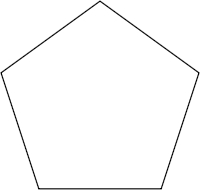
\includegraphics[width=2.5cm]{pentagone.jpg}
\hfill
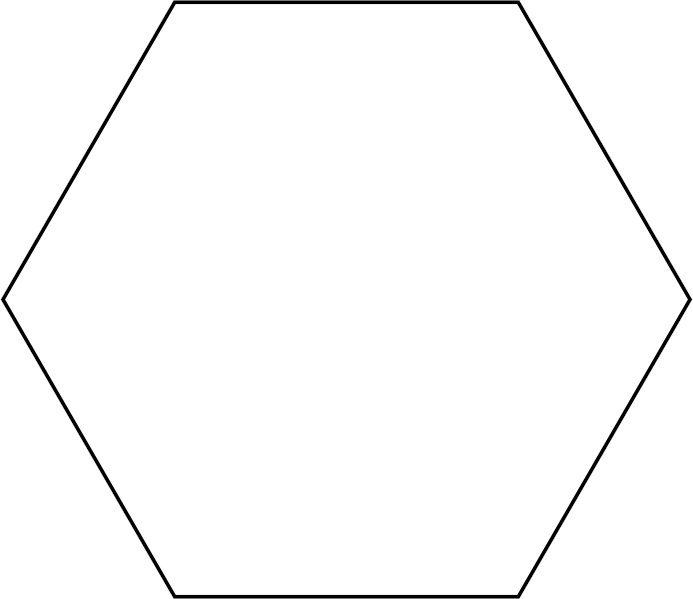
\includegraphics[width=2.5cm]{hexagone.jpg}
\hfill
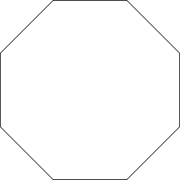
\includegraphics[width=2.5cm]{octogone.jpg}
}
\end{fig}
\end{minipage}

\end{td}

%-------------------------------------------------------------------------
\subsection{Analyser}\label{sub:analyser}
%-------------------------------------------------------------------------
\begin{td}[La multiplication «~à la russe~»]\label{td:russe}\index{multiplication « à la russe »}\index[td]{multiplication « à la russe »}
\em
La technique de multiplication dite «~à la rus\-se~» consiste à diviser par 
2 le multiplicateur (et ensuite les quotients obtenus), 
jusqu'à un quotient nul, à noter les restes,
et à multiplier parallèlement le multiplicande par 2. 
On additionne alors les multiples obtenus du multiplicande 
correspondant aux restes non nuls.

\noindent\begin{minipage}[t]{14cm}
\noindent Exemple : \begin{minipage}[t]{10cm}
$68 \times 123\ (= 8364)$\\
\begin{tabular}{|r|r|r|r|}
\hline
multiplicande & multiplicateur & reste      & somme partielle\\
$M \times 2$  & $m \div 2$     & $m \bmod 2$ &       \\
\hline
123  & 68 &   0   &   $(0\times 123) + 0$ \\
246  & 34 &   0   &   $(0\times 246) + 0$ \\
492  & 17 &   1   &   $(1\times 492) + 0$ \\
984  &  8 &   0   &   $(0\times 984) + 492$  \\
1968 &  4 &   0   &   $(0\times 1968) + 492$ \\
3936 &  2 &   0   &   $(0\times 3936) + 492$ \\
7872 &  1 &   1   &   $(1\times 7872) + 492$ \\
\hline
\multicolumn{3}{|r|}{$68 \times 123 =$} & 8364\\
\hline
\end{tabular}
\end{minipage}
\end{minipage}
\hfill
\begin{minipage}[t]{8cm}\footnotesize
\begin{rem}La multiplication en Egypte antique.\\[1mm]
\begin{minipage}{4cm}
La multiplication «~à la rus\-se~»
est une variante connue d'une technique égyptienne
décrite dans le papyrus Rhind (environ -1650). Le scribe Ahmès
y expose des problèmes de géométrie et d'arithmétique (qui viennent en partie 
des Babyloniens) dont cette technique de multiplication.
\end{minipage}
\hfill
\begin{minipage}{3.6cm}
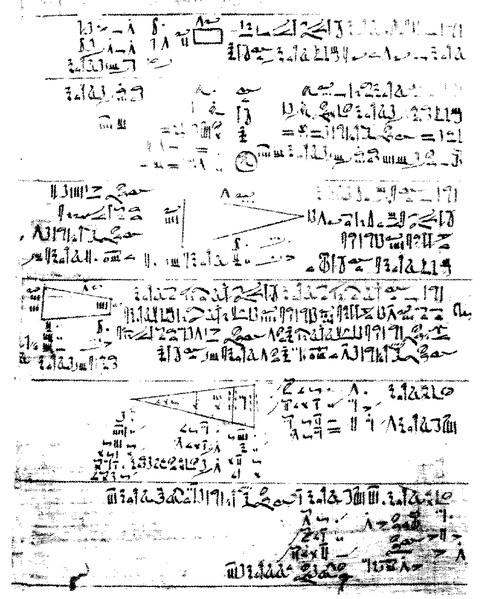
\includegraphics[width=3.5cm]{papyrus.jpg}
\end{minipage}
\end{rem}
\end{minipage}
\vspace*{3mm}

Effectuer les multiplications suivantes selon la technique «~à la russe~».
\begin{enumerate}
\item $64 \times 96\ (= 6144)$
\item $45 \times 239\ (= 10755)$
\end{enumerate}

\end{td} 

\begin{td}[La multiplication arabe]\label{td:ibnalbanna}
\index{multiplication arabe}\index[td]{multiplication arabe}
\em
On consid\`ere ici le texte d'Ibn al-Banna concernant la multiplication
\`a l'aide de tableaux  \cite{chabert}.

\begin{minipage}{15cm}
\footnotesize\em
« Tu construis un quadrilat\`ere que tu subdivises verticalement et
horizontalement en autant de bandes qu'il y a de positions dans les
deux nombres multipli\'es. Tu divises diagonalement les carr\'es
obtenus, \`a l'aide de diagonales allant du coin inf\'erieur gauche au
coin sup\'erieur droit (figure \ref{fig:ibnalbanna}).

Tu places le multiplicande au-dessus du quadrilat\`ere, en faisant 
correspondre chacune de ses positions \`a une colonne\footnote{L'écriture
du nombre s'effectue de droite à gauche (exemple : 352 s'écrira donc 253).}. 
Puis, tu places le multiplicateur \`a gauche ou \`a droite du quadrilat\`ere,
de telle sorte qu'il descende avec lui en faisant correspondre \'egalement 
chacune de ses positions \`a une ligne\footnote{L'écriture
du nombre s'effectue de bas en haut (exemple : {\tiny$\begin{array}{c}3\\5\\2\end{array}$} 
s'écrira donc {\tiny$\begin{array}{c}2\\5\\3\end{array}$}).}. 

Puis, tu multiplies, 
l'une apr\`es l'autre, chacune des positions du multiplicande du carr\'e 
par toutes les positions du multiplicateur, et tu poses le r\'esultat 
partiel correspondant \`a chaque position dans le carr\'e o\`u se coupent 
respectivement leur colonne et leur ligne, en pla\c{c}ant les unit\'es 
au-dessus de la diagonale et les dizaines en dessous. Puis, tu
commences \`a additionner, en partant du coin sup\'erieur gauche :
tu additionnes ce qui est entre les diagonales, sans effacer, 
en pla\c{c}ant chaque nombre dans sa position, en transf\'erant 
les dizaines de chaque somme partielle \`a la diagonale suivante et
en les ajoutant \`a ce qui y figure. 

La somme que tu obtiendras sera le r\'esultat. »
\end{minipage}
\hfill
\begin{minipage}{8cm}
\begin{fig}[Tableau d'Ibn al-Banna]\label{fig:ibnalbanna}
\mbox{}\\
\centerline{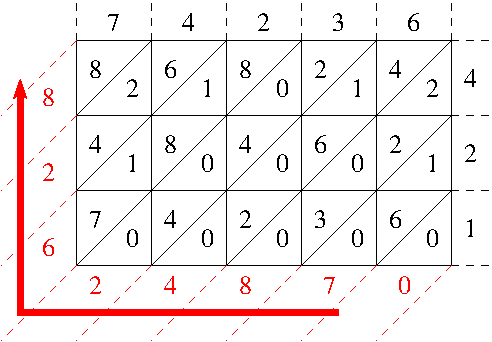
\includegraphics[width=7.5cm]{ibnalbanna.pdf}}
\end{fig}
\end{minipage}

En utilisant la m\'ethode du tableau d'Ibn al-Banna, calculer $63247\times124$ 
($= 7842628$).
\end{td}

\begin{td}[La division chinoise]\label{td:boulier}
\index{division chinoise}\index[td]{division chinoise}
\em
Dans sa version actuelle, le boulier chinois se compose d'un nombre variable de tringles
serties dans un cadre rectangulaire \cite{chabert}. Sur chacune de ces tringles, deux étages de boules
séparées par une barre transversale peuvent coulisser librement (figure \ref{fig:boulier}).
La notation des nombres repose sur le principe de la numération de position : chacune
des 2 boules du haut vaut 5 unités et chacune des 5 boules du bas vaut 1 unité. Seules
comptent les boules situées dans la région transversale.


\noindent
\begin{minipage}[t]{14cm}
Il existe des règles spéciales de division pour chaque diviseur de 1 à 9.
On consid\`ere ici les 7 r\`egles de division par 7 (figure \ref{fig:div7}) :\\
\noindent\begin{minipage}[t]{7cm}\footnotesize
\begin{enumerate}
\item {\em «~qi-yi xia jia san~»} : 7-1 ? ajouter 3 en dessous ! \\
\item {\em «~qi-er xia jia liu~»} : 7-2 ? ajouter 6 en dessous ! \\
\item {\em «~qi-san si sheng er~»} : 7-3 ? 4 reste 2 ! \\
\end{enumerate}
\end{minipage}\hfill
\begin{minipage}[t]{7cm}\footnotesize
\begin{enumerate}\setcounter{enumi}{3}
\item {\em «~qi-si wu sheng wu~»} : 7-4 ? 5 reste 5 ! \\
\item {\em «~qi-wu qi sheng yi~»} : 7-5 ? 7 reste 1 ! \\
\item {\em «~qi-liu ba sheng si~»} : 7-6 ? 8 reste 4 ! \\
\item {\em «~feng-qi jin yi~»} : 7-7 ? 1 monté ! \\
\end{enumerate}
\end{minipage}
\end{minipage}
\hfill
\begin{minipage}[t]{8cm}
\begin{fig}[Boulier chinois]\label{fig:boulier}
\mbox{}\\
\centerline{\em
\mbox{}\hfill 8017 :\hfill
\begin{minipage}{5cm}
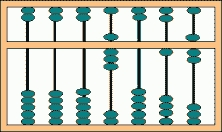
\includegraphics[width=4cm]{boulier.jpg}
\end{minipage}}
\end{fig}
\end{minipage}

\noindent
\begin{minipage}[t]{15cm}
Ces règles ne sont pas des règles logiques, 
mais de simples procédés mnémotechniques
indiquant ce qu'il convient de faire selon la situation. Leur énoncé débute par le
rappel du diviseur, ici 7, et se poursuit par l'énoncé du dividende, par exemple 3 :
7-3. Le reste de la règle indique quelles manipulations effectuées, ajouts ou retraits
de boules. Il faut également savoir que le dividende étant posé sur le boulier, on doit
appliquer les règles aux chiffres successifs du dividende, en commençant par celui dont
l'ordre est le plus élevé.
«~ajouter en dessous~» veut dire «~mettre des boules au rang 
immédiatement inférieur (à droite) au rang considéré~» et «~monter~» veut dire «~mettre des boules
au rang immédiatement supérieur (à gauche) au rang considéré~».

Pour effectuer la division d'un nombre par 7, on pose le dividende à droite sur le
boulier et le diviseur (7) à gauche. On opère sur les chiffres successifs du dividende
en commençant par celui d'ordre le plus élevé (le plus à gauche). Les règles
précédemment énoncées sont appliquées systématiquement.

Utiliser un boulier chinois pour diviser 1234 par 7 ($1234 = 176\times 7 + 2$).

\centerline{\begin{tabular}{cccccc}
1 & \makebox[1mm]{} & 0 & 0 & 0 & 0 \\
\hline
2 & & 1 & 2 & 3 & 4
\end{tabular}
$\rightarrow$
\begin{tabular}{cccccc}
1 & \makebox[1mm]{} & 0 & 1 & 1 & 0 \\
\hline
2 & & 1 & 2 & 1 & 2
\end{tabular}}
\end{minipage}
\hfill
\begin{minipage}[t]{8cm}\footnotesize
\begin{fig}[Règles de la division par 7]\label{fig:div7}
\mbox{}\\
\centerline{\em\begin{tabular}{|c|c|c|}
\hline
Règle & Avant & Après \\
\hline
\hline
7-1   & 
\begin{tabular}{ccccc}
1 & \makebox[0.5mm]{} & 0 & 0 & 0 \\
\hline
2 & & 0 & 1 & 0
\end{tabular} &
\begin{tabular}{ccccc}
1 & \makebox[0.5mm]{} & 0 & 0 & 0 \\
\hline
2 & & 0 & 1 & 3
\end{tabular} \\
\hline
\hline
7-2   & 
\begin{tabular}{ccccc}
1 & \makebox[0.5mm]{} & 0 & 0 & 0 \\
\hline
2 & & 0 & 2 & 0
\end{tabular} &
\begin{tabular}{ccccc}
1 & \makebox[0.5mm]{} & 0 & 0 & 1 \\
\hline
2 & & 0 & 2 & 1
\end{tabular} \\
\hline
\hline
7-3   & 
\begin{tabular}{ccccc}
1 & \makebox[0.5mm]{} & 0 & 0 & 0 \\
\hline
2 & & 0 & 3 & 0
\end{tabular} &
\begin{tabular}{ccccc}
1 & \makebox[0.5mm]{} & 0 & 0 & 0 \\
\hline
2 & & 0 & 4 & 2
\end{tabular} \\
\hline
\hline
7-4   & 
\begin{tabular}{ccccc}
1 & \makebox[0.5mm]{} & 0 & 0 & 0 \\
\hline
2 & & 0 & 4 & 0
\end{tabular} &
\begin{tabular}{ccccc}
1 & \makebox[0.5mm]{} & 0 & 1 & 1 \\
\hline
2 & & 0 & 0 & 0
\end{tabular} \\
\hline
\hline
7-5   & 
\begin{tabular}{ccccc}
1 & \makebox[0.5mm]{} & 0 & 1 & 0 \\
\hline
2 & & 0 & 0 & 0
\end{tabular} &
\begin{tabular}{ccccc}
1 & \makebox[0.5mm]{} & 0 & 1 & 0 \\
\hline
2 & & 0 & 2 & 1
\end{tabular} \\
\hline
\hline
7-6   & 
\begin{tabular}{ccccc}
1 & \makebox[0.5mm]{} & 0 & 1 & 0 \\
\hline
2 & & 0 & 1 & 0
\end{tabular} &
\begin{tabular}{ccccc}
1 & \makebox[0.5mm]{} & 0 & 1 & 0 \\
\hline
2 & & 0 & 3 & 4
\end{tabular} \\
\hline
\hline
7-7   & 
\begin{tabular}{ccccc}
1 & \makebox[0.5mm]{} & 0 & 1 & 0 \\
\hline
2 & & 0 & 2 & 0
\end{tabular} &
\begin{tabular}{ccccc}
1 & \makebox[0.5mm]{} & 0 & 0 & 0 \\
\hline
2 & & 1 & 0 & 0
\end{tabular} \\
\hline
\end{tabular}}
\end{fig}
\end{minipage}
\end{td}

\begin{td}[Le calcul Shadok]\label{td:shadok}\index{calcul {{\sc Shadok}}}\index[td]{calcul {{\sc Shadok}}}
\em
Les cerveaux des Shadoks avaient une capacité tout à fait limitée \cite{rouxel}.
Ils ne comportaient en tout que 4 cases.
Comme ils n'avaient que 4 cases, évidemment les Shadoks ne connaissaient 
pas plus de 4 mots :  {\sc ga, bu, zo et meu} (figure \ref{fig:bdShadok}).
Etant donné qu'avec 4 mots, ils ne pouvaient pas compter plus loin que 4,
le Professeur Shadoko avait réformé tout ça :
\begin{itemize}
\item Quand il n'y a pas de Shadok, on dit {\sc ga} et on écrit {\sc ga}.
\item Quand il y a un Shadok de plus, on dit {\sc bu} et on écrit {\sc bu}.
\item Quand il y a encore un Shadok, on dit {\sc zo} et on écrit {\sc zo}.
\item Et quand il y en a encore un autre, on dit {\sc meu} et on écrit {\sc meu}.
\end{itemize}
Tout le monde applaudissait très fort et trouvait ça génial sauf le Devin Plombier 
qui disait qu'on n'avait pas idée d'inculquer à des enfants des bêtises pareilles 
et que Shadoko, il fallait le condamner. 
Il fut très applaudi aussi. Les mathématiques, 
cela les intéressait, bien sûr, mais brûler le professeur, c'était intéressant aussi, faut dire. 
Il fut décidé à l'unanimité qu'on le laisserait parler et qu'on le brûlerait après, à la récréation.
\begin{itemize}
\item Répétez avec moi : {\sc meu} {\sc zo} {\sc bu} {\sc ga}\ldots {\sc ga} {\sc bu} {\sc zo} {\sc meu}.
\item Et après! ricanait le Plombier.
\item Si je mets un Shadok en plus, évidemment, je n'ai plus assez 
de mots pour les compter, alors c'est très simple : on les jette dans une poubelle, 
et je dis que j'ai {\sc bu} poubelle. Et pour ne pas confondre avec le {\sc bu} du début, 
je dis qu'il n'y a pas de Shadok à côté de la poubelle et j'écris {\sc bu} {\sc ga}. 
{\sc bu} Shadok à côté de la poubelle: {\sc bu} {\sc bu}. Un autre : {\sc bu} {\sc zo}. Encore un autre : {\sc bu} {\sc meu}. 
On continue. {\sc zo} poubelles et pas de Shadok à côté : {\sc zo} {\sc ga}\ldots 
{\sc meu} poubelles et {\sc meu} Shadoks à côté : {\sc meu} {\sc meu}. 
Arrivé là, si je mets un Shadok en plus, il me faut une autre poubelle. 
Mais comme je n'ai plus de mots pour compter les poubelles, je m'en débarrasse 
en les jetant dans une grande poubelle. 
J'écris {\sc bu} grande poubelle avec pas de petite poubelle 
et pas de Shadok à côté: {\sc bu} {\sc ga} {\sc ga}, et on continue\ldots {\sc bu} {\sc ga} {\sc bu}, 
{\sc bu} {\sc ga} {\sc zo}\ldots {\sc meu} {\sc meu} {\sc zo}, {\sc meu} {\sc meu} {\sc meu}.
Quand on arrive là et qu'on a trop de grandes poubelles pour pouvoir les compter, 
eh bien, on les met dans une super-poubelle, on écrit {\sc bu} {\sc ga} {\sc ga} {\sc ga}, 
et on continue\ldots (figure \ref{fig:calculShadok}).
\end{itemize}

\noindent
\begin{minipage}[t]{8cm}
\begin{enumerate}
\item Quels sont les entiers décimaux représentés en «~base Shadok~» 
	par les expressions suivantes ?
	\begin{enumerate}
	\item {\sc ga} {\sc ga}
	\item {\sc bu} {\sc bu} {\sc bu}
	\item {\sc zo} {\sc zo} {\sc zo} {\sc zo}
	\item {\sc meu} {\sc meu} {\sc meu} {\sc meu} {\sc meu} 
	\end{enumerate}	
\item Effectuer les calculs Shadok suivants.
	\begin{enumerate}
	\item {\sc zo} {\sc zo} {\sc meu} $+$ {\sc bu} {\sc ga} {\sc meu}
	\item {\sc meu} {\sc ga} {\sc meu} $-$ {\sc bu} {\sc meu} {\sc ga}
	\item {\sc zo} {\sc meu} {\sc meu} $\times$ {\sc bu} {\sc ga} {\sc meu}
	\item {\sc zo} {\sc zo} {\sc zo} {\sc meu} $\div$ {\sc bu} {\sc ga} {\sc zo}
	\end{enumerate}
\end{enumerate}
\end{minipage}
\hfill
\begin{minipage}[t]{8cm}
\begin{fig}[Les Shadoks : {\sc ga} {\sc bu} {\sc zo} {\sc meu}]\label{fig:bdShadok}
\mbox{}\\
\centerline{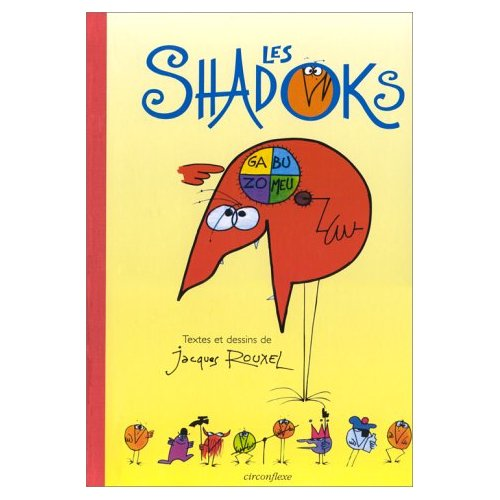
\includegraphics[width=3.75cm]{bdShadok.jpg}}
\end{fig}
\end{minipage}
\hfill
\begin{minipage}[t]{8cm}
\begin{fig}[Les 18 premiers nombres Shadok]\label{fig:calculShadok}
\mbox{}\\
\centerline{\begin{tabular}[t]{l@{ : }ll@{ : }ll@{ : }l}
0 & {\sc ga} 	      & 6  & {\sc bu} {\sc zo}  & 12 & {\sc meu} {\sc ga}\\
1 & {\sc bu} 	      & 7  & {\sc bu} {\sc meu} & 13 & {\sc meu} {\sc bu}\\
2 & {\sc zo} 	      & 8  & {\sc zo} {\sc ga}  & 14 & {\sc meu} {\sc zo}\\
3 & {\sc meu} 	      & 9  & {\sc zo} {\sc bu}  & 15 & {\sc meu} {\sc meu}\\
4 & {\sc bu} {\sc ga} & 10 & {\sc zo} {\sc zo}  & 16 & {\sc bu} {\sc ga} {\sc ga}\\
5 & {\sc bu} {\sc bu} & 11 & {\sc zo} {\sc meu} & 17 & {\sc bu} {\sc ga} {\sc bu}\\
\end{tabular}}
\end{fig}
\end{minipage}
\end{td}

%-------------------------------------------------------------------------
\newpage
\subsection{Solutions des exercices}\label{sub:solutionsIntro}
%-------------------------------------------------------------------------
\begin{description}
\item[TD \ref{td:qcmIntro} :] QCM (1).\\
	Les bonnes réponses sont extraites directement
	du texte de la section \ref{contexte} : \\
	1a, 2e, 3b, 4b, 5e, 6e, 7a, 8d
\item[TD \ref{td:mips} :] Puissance de calcul.\index{matériel!mips}\\
	L'unité de puissance est donné ici en Mips («~million d'instructions par
	seconde~»).
	\begin{enumerate}
	\item le premier micro-ordinateur de type PC : $\approx 10^{-1}$ Mips
	\item une console de jeu actuelle : $\approx 10^{4}$ Mips
	\item un micro-ordinateur actuel : $\approx 10^{4}$ Mips
	\item {\em Deeper-Blue} : l'ordinateur qui a « battu » Kasparov aux 
		échecs en 1997 : $\approx 10^{7}$ Mips
	\item le plus puissant ordinateur actuel : $\approx 10^{9}$ Mips
	\end{enumerate}
\item[TD \ref{td:stock} :] Stockage de données.\index{octet}

	\begin{enumerate}
	\item une page d'un livre : $\approx$ 50 lignes de 80 caractères = 4 ko
	\item une encyclopédie en 20 volumes : $\approx$ 20 volumes de 1000
	pages de 50 lignes de 80 caractères = 80 Mo (sans images !)
	\item une photo couleur : $\approx$ de 1Mo à 100 Mo selon la qualité
	\item une heure de vidéo : $\approx$ de 500 Mo à 2 Go 
		selon la qualité vidéo (DivX, MPEG-2\ldots)
	\item une minute de son : $\approx$ de 1 Mo (MP3) à 10 Mo 
		selon la qualité du son
	\item une heure de son : $\approx$ de 60 Mo à 600 Mo 
		selon la qualité du son
	\end{enumerate}

	\begin{rem}Loi de Moore.\index{{{\sc Moore}}}\index{matériel!loi de {{\sc Moore}}}\\
	\begin{minipage}{8cm}
	\centerline{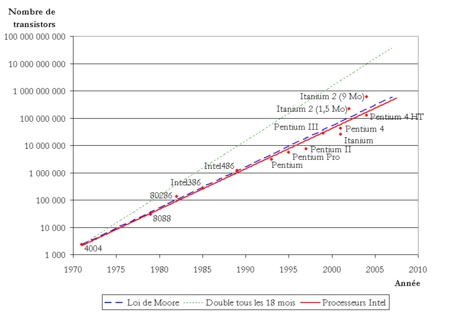
\includegraphics[width=7cm]{loimoore.jpg}}
	\end{minipage}
	\hfill
	\begin{minipage}{15cm}
	Gordon Earl Moore est le co-fondateur avec Robert Noyce et Andrew Grove de la société Intel en 1968 
	(fabriquant n°1 mondial de microprocesseurs).
	En 1965, il expliquait que la complexité des semiconducteurs 
	doublait tous les dix-huit mois à coût constant depuis 1959, date de leur invention. 
	En 1975, il précise sa «~première loi~» en affirmant que le nombre de transistors des microprocesseurs  
	sur une puce de silicium double tous les deux ans («~deuxième loi~»).
	\end{minipage}
	\end{rem}


\item[TD \ref{td:plage3} :] Dessins sur la plage : exécution.
	\begin{enumerate}
	\item On trace un triangle rectangle dont l'hypothénuse fait 5 pas de long
		(d'après le théorème de Pythagore : $5^2 = 3^2 + 4^2$).
	\item On a donc marché $3 + 4 + 5 = 12$ pas.
	\end{enumerate}
%\newpage
\item[TD \ref{td:plage4} :] Dessins sur la plage : conception.

	\noindent\begin{minipage}{15cm}
	Imaginons l'algorithme de tracé suivant :
	\begin{enumerate}
	\item avance de 2 pas,
	\item tourne à gauche de $90^\circ$,
	\item avance de 3 pas,
	\item tourne à gauche de $90^\circ$,
	\item avance de 4 pas,
	\item tourne à gauche de $90^\circ$,
	\item avance de 5 pas,
	\item tourne à gauche de $90^\circ$,
	\item avance de 6 pas.
	\end{enumerate}
		\end{minipage}
	\hfill
	\begin{minipage}{8cm}
	\begin{fig}[Spirales rectangulaires]\label{fig:spirale}
	\mbox{}\\
	\centerline{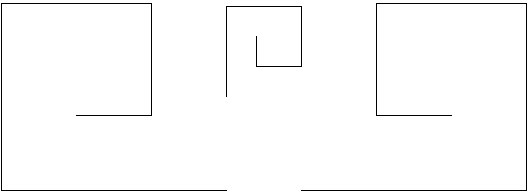
\includegraphics[width=7.5cm]{spirale.pdf}}
	\end{fig}
	\end{minipage}
	\vspace*{3mm}
	
	\begin{description}
	\item[validité :] on doit au moins vérifier que la figure obtenue à toutes
		les caractéristiques recherchées : spirale rectangulaire de
		5 côtés, le plus petit côté faisant 2 pas de long et chaque 
		côté fait un pas de plus que le précédent (figure \ref{fig:spirale}).
	\item[robustesse :] cet algorithme suppose qu'on a suffisamment de place pour
		tracer une spirale (le dernier côté fait 6 pas de long); s'il fonctionne 
		correctement sur une plage, il ne fonctionnera certainement plus dans un
		placard.
	\item[réutilisabilité :] il existe une infinité de spirales rectangulaires
		qui ont les caractéristiques attendues; il suffit de penser
		à changer l'orientation initiale ou la longueur du pas par exemple. 
		On ne pourra donc pas utiliser l'algorithme tel quel dans toutes les
		configurations : il aurait fallu paramétrer l'angle de rotation et la
		longueur du pas.
	\item[complexité :] on peut la caractériser par le nombre de pas : 
		$2 + 3 + 4 + 5 + 6 = 20$ pas.
	\item[efficacité :] si la complexité se calcule en nombre de pas comme
		ci-dessus, on pourrait imaginer par exemple que la fréquence des
		pas soit plus grande («~fréquence d'horloge~») ou que 
		5 personnes prennent en charge chacune un côté de la spirale 
		pour gagner du temps («~système multi-processeurs~»).
	\end{description}
\newpage
\item[TD \ref{td:tortue} :] Tracés de polygones réguliers.\index[algo]{polygones réguliers}
	\begin{enumerate}
	\item Pentagone régulier de 10 pas de côté.\\
		\begin{minipage}{6cm}
		\begin{enumerate}
		\item avance de 10 pas,
		\item tourne à gauche de $(360/5)^\circ$,
		\item avance de 10 pas,
		\item tourne à gauche de $(360/5)^\circ$,
		\item avance de 10 pas,
		\item tourne à gauche de $(360/5)^\circ$,
		\item avance de 10 pas,
		\item tourne à gauche de $(360/5)^\circ$,
		\item avance de 10 pas,
		\item tourne à gauche de $(360/5)^\circ$.
		\end{enumerate}
		\end{minipage}
		\hfill
		\begin{minipage}{7cm}
		On remarque qu'on a effectué 5 fois de suite les 2 instructions 
		suivantes :
		\begin{enumerate}
		\item avance de 10 pas,
		\item tourne à gauche de $(360/5)^\circ$.
		\end{enumerate}
		Pour simplifier, on écrira plutôt :\\
		Répète 5 fois de suite les 2 instructions
		\begin{enumerate}
		\item avance de 10 pas,
		\item tourne à gauche de $(360/5)^\circ$.
		\end{enumerate}
		C'est ce que nous ferons dans les exemples suivants.
		\end{minipage}
	\item Hexagone régulier de 10 pas de côté.\\
		Répète 6 fois de suite les 2 instructions 
		\begin{enumerate}
		\item avance de 10 pas,
		\item tourne à gauche de $(360/6)^\circ$,
		\end{enumerate}
	\item Octogone régulier de 10 pas de côté.\\
		Répète 8 fois de suite les 2 instructions 
		\begin{enumerate}
		\item avance de 10 pas,
		\item tourne à gauche de $(360/8)^\circ$,
		\end{enumerate}
	\item Polygone régulier de $n$ côtés de 10 pas chacun.\\
		Répète $n$ fois de suite les 2 instructions 
		\begin{enumerate}
		\item avance de 10 pas,
		\item tourne à gauche de $(360/n)^\circ$,
		\end{enumerate}
	\end{enumerate}
\newpage
\item[TD \ref{td:russe} :] Multiplication «~à la russe~».\index{multiplication « à la russe »}
	
	\noindent
	\begin{minipage}[t]{12cm}
	\begin{enumerate}
	\item \begin{tabular}[t]{|r|r|r|r|}
		\hline
		multiplicande & multiplicateur & reste      & somme partielle\\
		$M \times 2$  & $m \div 2$     & $m \bmod 2$ &       \\
		\hline
		 96  & 64 &   0   &   $(0\times 96) + 0$ \\
		192  & 32 &   0   &   $(0\times 192) + 0$ \\
		384  & 16 &   0   &   $(1\times 384) + 0$ \\
		768  &  8 &   0   &   $(0\times 768) + 0$  \\
	       1536  &  4 &   0   &   $(0\times 1536) + 0$ \\
	       3072  &  2 &   0   &   $(0\times 3072) + 0$ \\
	       6144  &  1 &   1   &   $(1\times 6144) + 0$ \\
		\hline
		\multicolumn{3}{|r|}{$64 \times 96 =$} & 6144\\
		\hline
		\end{tabular}
	\end{enumerate}
	\end{minipage}
	\hfill
	\begin{minipage}[t]{12cm}
	\begin{enumerate}\setcounter{enumi}{1}
	\item \begin{tabular}[t]{|r|r|r|r|}
		\hline
		multiplicande & multiplicateur & reste      & somme partielle\\
		$M \times 2$  & $m \div 2$     & $m \bmod 2$ &       \\
		\hline
		239  & 45 &   1   &   $(1\times 239) + 0$ \\
		478  & 22 &   0   &   $(0\times 478) + 239$ \\
		956  & 11 &   1   &   $(1\times 956) + 239$ \\
	       1912  &  5 &   1   &   $(1\times 1912) + 1195$  \\
	       3824  &  2 &   0   &   $(0\times 3824) + 3107$ \\
	       7648  &  1 &   1   &   $(1\times 7648) + 3107$ \\
		\hline
		\multicolumn{3}{|r|}{$45 \times 239 =$} & 10755\\
		\hline
		\end{tabular}
	\end{enumerate}
	\end{minipage}
	\vspace*{2mm}
	
\item[TD \ref{td:ibnalbanna} :] Multiplication arabe : $63247\times124 = 7842628$.\index{multiplication arabe}

	\vspace*{3mm}
	
	{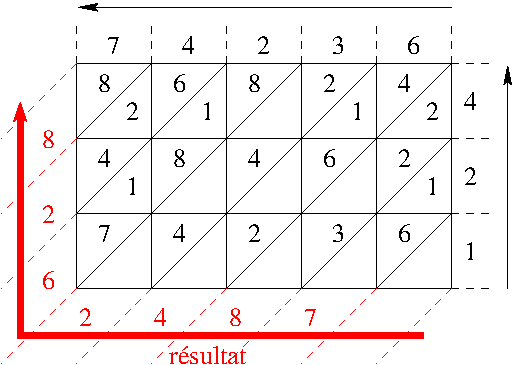
\includegraphics[width=7cm]{ibnalbanna1.pdf}} 

	
\item[TD \ref{td:boulier} :] Division chinoise : $1234 \div 7$ 
	($1234 = 176\times 7 +2$).\index{division chinoise}
	
	\vspace*{3mm}
	
	{\footnotesize
	\begin{tabular}{|cccccc|}
	\hline
	  &                 & $\downarrow$ & & & \\
	1 & \makebox[1mm]{} & 0 & 0 & 0 & 0 \\
	\hline
	2 & & 1 & 2 & 3 & 4 \\
	\hline
	\end{tabular}
	$\rightarrow$ 7-1 $\rightarrow$ 
	\begin{tabular}{|cccccc|}
	\hline
	  &                 & & $\downarrow$ & & \\
	1 & \makebox[1mm]{} & 0 & 1 & 0 & 0 \\
	\hline
	2 & & 1 & 0 & 3 & 4\\
	\hline
	\end{tabular}
	$\rightarrow$ 7-5 $\rightarrow$ 
	\begin{tabular}{|cccccc|}
	\hline
	  &                 & & & $\downarrow$ & \\
	1 & \makebox[1mm]{} & 0 & 1 & 0 & 0 \\
	\hline
	2 & & 1 & 2 & 4 & 4\\
	\hline
	\end{tabular}
	$\rightarrow$ 7-4 $\rightarrow$ 
	\begin{tabular}{|cccccc|}
	\hline
	  &                 & & & & $\downarrow$ \\
	1 & \makebox[1mm]{} & 0 & 1 & 1 & 1 \\
	\hline
	2 & & 1 & 2 & 0 & 4\\
	\hline
	\end{tabular}
	$\rightarrow$ 7-7 $\rightarrow$ 
	\begin{tabular}{|cccccc|}
	\hline
	  &                 & & & & \\
	1 & \makebox[1mm]{} & 0 & 1 & 1 & 0 \\
	\hline
	2 & & 1 & 2 & 1 & 2\\
	\hline
	\end{tabular}
	}
	
%	\begin{rem}Boulier chinois : division par 3.%
%	\begin{enumerate}
%	\item {\em «~san-yi sanshi-yi~»} : trois-un ? trente et un ! \\
%		(on pose 3 \`a la place du 1, et on ajoute 1 \`a droite)
%	\item {\em «~san-er liushi-er~»} : trois-deux ? soixante deux ! \\
%		(on pose 6 \`a la place du 2, et on ajoute 2 \`a droite)
%	\item {\em «~feng san jin yi-shi~»} : trois-trois ? dizaine mont\'ee ! \\
%		(on pose 0 \`a la place du 3, et on ajoute 1 \`a gauche)
%	\end{enumerate}
%	Effectuer la division $2271 \div 3$ avec le boulier chinois.
%	\end{rem}
\newpage	
\item[TD \ref{td:shadok} :] Calcul Shadok.\index{calcul {{\sc Shadok}}}

	\begin{rem}
	Un entier positif en base $b$ est représenté par une suite de
	chiffres {$(r_nr_{n-1}\ldots r_1r_0)_b$}
	où les $r_i$ sont des chiffres de la base $b$ ($0\leq r_i < b$).
	Ce nombre a pour valeur:
	$${r_nb^n + r_{n-1}b^{n-1} + \ldots + r_1b^1 + r_0b^0 = 
        \sum^{i=n}_{i = 0} r_ib^i}$$
	
	Un nombre fractionnaire (nombre avec des chiffres après la virgule :
	{$(r_nr_{n-1}\ldots r_1r_0.r_{-1}r_{-2}\ldots)_b$})
	est défini sur un sous-en\-semble borné, incomplet et fini des rationnels.
	Un tel nombre a pour valeur :
	$${r_nb^n + r_{n-1}b^{n-1} + \ldots + r_0b^0 + r_{-1}b^{-1} + r_{-2}b^{-2} + \ldots}$$
	En pratique, le nombre de chiffres après la virgule est limité par la taille physique
	en machine.
	$${(r_nr_{n-1}\ldots r_1r_0.r_{-1}r_{-2}\ldots r_{-m})_b = \sum_{i=-m}^{i=n} r_ib^i}$$
	\end{rem}
	
	Le système Shadok est un système de numération en base 4 :\\
	{\sc ga} = 0, {\sc bu} = 1, {\sc zo} = 2 et {\sc meu} = 3.
	\begin{enumerate}
	\item   \begin{enumerate}
		\item {\sc ga} {\sc ga} 
			$= (00)_4 = 0$
		\item {\sc bu} {\sc bu} {\sc bu} 
			$= (111)_4 = 1\cdot 4^2 + 1\cdot 4^1 + 1\cdot 4^0 = 16 + 4 + 1 = 21$
		\item {\sc zo} {\sc zo} {\sc zo} {\sc zo} 
			$= (2222)_4 = 2\cdot 4^3 + 2\cdot 4^2 + 2\cdot 4^1 + 2\cdot 4^0 = 128 + 32 + 8 + 2 = 170$
		\item {\sc meu} {\sc meu} {\sc meu} {\sc meu} {\sc meu} 
			$= (33333)_4 = 3 \cdot 4^4 + 3\cdot 4^3 + 3\cdot 4^2 + 3\cdot 4^1 + 3\cdot 4^0 = 768 + 192 + 48 + 12 + 3 =
			1023$
		\end{enumerate}	
	\item	\begin{enumerate}
		\item {\sc zo} {\sc zo} {\sc meu} $+$ {\sc bu} {\sc ga} {\sc meu} 
			$= (223)_4 + (103)_4 = (332)_4 = 43 + 19 = 62$
		\item {\sc meu} {\sc ga} {\sc meu} $-$ {\sc bu} {\sc meu} {\sc ga} 
			$= (303)_4 - (130)_4 = (113)_4 = 51 - 28 = 23$
		\item {\sc zo} {\sc meu} {\sc meu} $\times$ {\sc bu} {\sc ga} {\sc meu} 
			$= (233)_4 \times (103)_4 = (31331)_4 = 47 \times 19 = 893$
		\item {\sc zo} {\sc zo} {\sc zo} {\sc meu} $\div$ {\sc bu} {\sc ga} {\sc zo} 
			$= (2223)_4 \div (102)_4 = (21)_4 = 171 \div 18 = 9$
		\end{enumerate}
	\end{enumerate}
\end{description}

%-------------------------------------------------------------------------
\newpage
\setlength{\textwidth}{16cm}
\setlength{\linewidth}{16cm}
\setlength{\textheight}{16cm}
\setlength{\marginparwidth}{8cm}
\setlength{\marginparsep}{1cm}
\setlength{\oddsidemargin}{0cm}
\setlength{\evensidemargin}{+8cm}
\setlength{\topmargin}{-0.75cm}
\section{Annexes}
%-------------------------------------------------------------------------

%-------------------------------------------------------------------------
\subsection{Lettre de Jacques Perret}\label{annexe:perret}
%-------------------------------------------------------------------------
\marginpar{\footnotesize\em
\begin{fig}[Le premier ordinateur (1946)]\label{fig:eniac}
ENIAC (Electronic Numerical Integrator 
Analyser and Computer).
\mbox{}\\
\centerline{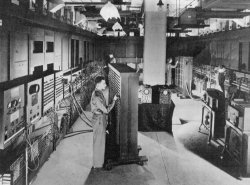
\includegraphics[width=6cm]{eniac2.jpg}}
\end{fig}
\begin{fig}[Premiers micro-ordinateurs]\label{fig:micros}
$$\begin{minipage}{6cm}
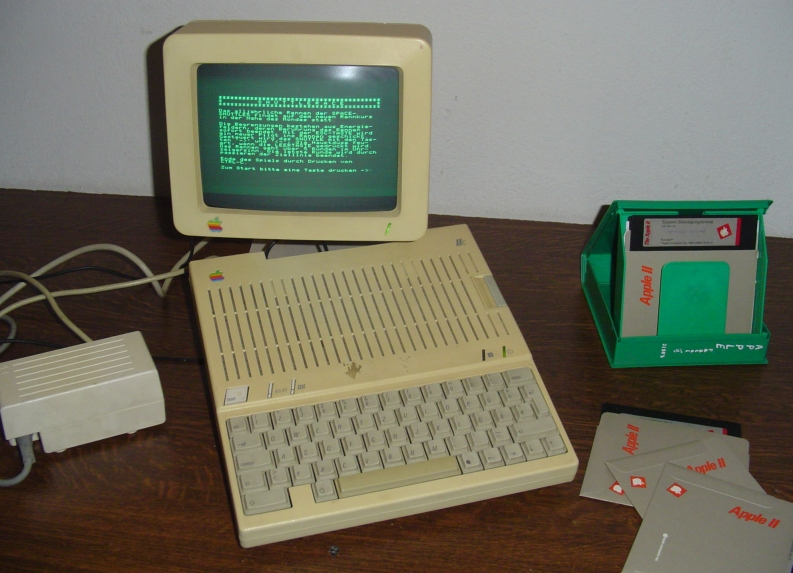
\includegraphics[width=2.25cm]{apple2.jpg}\hfill
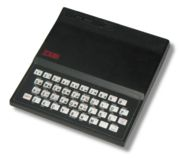
\includegraphics[width=2.25cm]{zx81.jpg}

\mbox{}\hfill Apple II (1977) \hfill ZX 81 (1981) \hfill \mbox{}

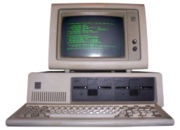
\includegraphics[width=2.25cm]{ibmpc.jpg}\hfill
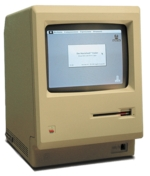
\includegraphics[width=2.25cm]{macintosh.jpg}

\mbox{}\hfill IBM PC (1981)\hfill Macintosh (1984)\hfill \mbox{}
\end{minipage}$$
\end{fig}}
Au printemps de 1955, IBM France s'apprêtait à construire dans ses ateliers 
de Corbeil-Essonnes (consacrés jusque-là au montage des machines mécanographiques 
--- tabulatrices, trieuses, \ldots --- de technologie électromécanique) 
les premières machines électroniques destinées au traitement de l'information. 
Aux États-Unis ces nouvelles machines étaient désignées sous le vocable 
Electronic Data Processing System. Le mot «~computer~» était plutôt réservé 
aux machines scientifiques et se traduisait aisément en «~calculateur~» ou «~calculatrice~».
Sollicité par la direction de l'usine de Corbeil-Essonnes, François Girard, 
alors responsable du service promotion générale publicité, 
décida de consulter un de ses anciens maîtres, Jacques Perret, professeur de philologie 
latine à la Sorbonne. A cet effet il écrit une lettre à la signature de C. de Waldner, 
président d'IBM France. Il décrit sommairement la nature et les fonctions des 
nouvelles machines. Il accompagne sa lettre de brochures illustrant les machines 
mécanographiques. Le 16 avril, le professeur Perret lui répond.
L'ordinateur IBM 650 peut commencer sa carrière.
Protégé pendant quelques mois par IBM France, le mot fut rapidement adopté
par un public de spécialistes, de chefs d'entreprises et par l'administration. 
IBM décida de le laisser dans le domaine public
(d'après le site de la $10^{\grave eme}$ semaine de la langue française et de la francophonie
\href{http://www.semainelf.culture.fr/site2005/dixmots}{\tt www.semainelf.culture.fr/site2005/dixmots}).

{\em\index{{{\sc Perret}}}
Le 16 IV 1955

Cher Monsieur,

Que diriez-vous d'«~ordinateur~» ?\index{ordinateur} C'est un mot correctement formé, qui se trouve même dans le
Littré comme adjectif désignant Dieu qui met de l'ordre dans le monde. Un mot de ce genre a
l'avantage de donner aisément un verbe «~ordiner~», un nom d'action «~ordination~». L'inconvénient
est que «~ordination~» désigne une cérémonie religieuse ; mais les deux champs de signification
(religion et comptabilité) sont si éloignés et la cérémonie d'ordination connue, je crois, de si peu de
personnes que l'inconvénient est peut-être mineur. D'ailleurs votre machine serait «~ordinateur~» (et
non ordination) et ce mot est tout à fait sorti de l'usage théologique. «~Systémateur~» serait un
néologisme, mais qui ne me paraît pas offensant ; il permet «~systématisé~» ; - mais «~système~» ne
me semble guère utilisable - «~combinateur~» a l'inconvénient du sens péjoratif de «~combine~» ;
«~combiner~» est usuel donc peu capable de devenir technique ; «~combination~» ne me paraît guère
viable à cause de la proximité de «~combinaison~». Mais les Allemands ont bien leurs «~combinats~»
(sorte de trusts, je crois), si bien que le mot aurait peut-être des possibilités autres que celles
qu'évoque «~combine~».

\marginpar{\footnotesize\em
\begin{fig}[Du 8086 (1978) au Core 2 (2006)]\label{fig:intel86}
$$\begin{minipage}{6cm}
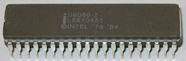
\includegraphics[width=2.25cm]{8086.jpg}\hfill
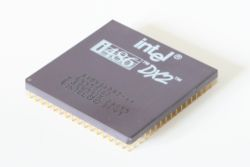
\includegraphics[width=2.25cm]{80486.jpg}

\mbox{}\hfill 8086 \hfill 80486 \hfill \mbox{}

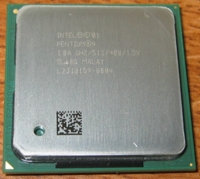
\includegraphics[width=2.25cm]{pentium4.jpg}\hfill
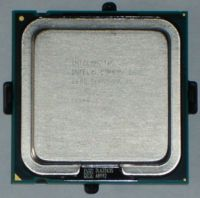
\includegraphics[width=2.25cm]{core2.jpg}

\mbox{}\hfill Pentium 4 \hfill Core Duo \hfill \mbox{}
\end{minipage}$$
\end{fig}

\begin{fig}[Micro-ordinateurs récents]\label{fig:derniersnes}
$$\begin{minipage}{6cm}
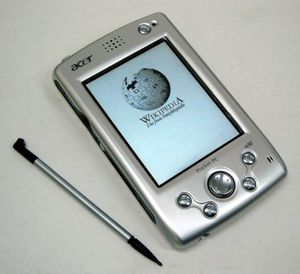
\includegraphics[width=2.25cm]{pda.jpg}\hfill
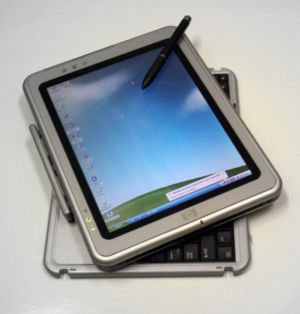
\includegraphics[width=2.25cm]{tablette.jpg}

\mbox{}\hfill PDA \hfill Tablette \hfill \mbox{}

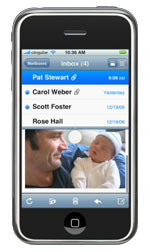
\includegraphics[width=1.5cm]{iphone.jpg}\hfill
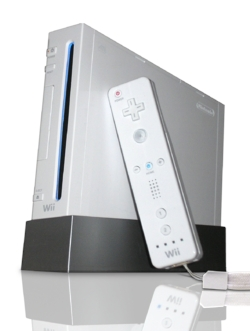
\includegraphics[width=2.25cm]{wii.jpg}

\mbox{}\hfill iPhone \hfill Wii \hfill \mbox{}
\end{minipage}$$
\end{fig}
}
«~Congesteur~», «~digesteur~» évoquent trop «~congestion~» et «~digestion~».
«~Synthé\-ti\-seur~» ne me
paraît pas un mot assez neuf pour designer un objet spécifique, déterminé comme votre machine.
En relisant les brochures que vous m'avez données, je vois que plusieurs de vos appareils sont
désignés par des noms d'agent féminins (trieuse, tabulatrice). «~Ordinatrice~» serait parfaitement
possible et aurait même l'avantage de séparer plus encore votre machine du vocabulaire de la
théologie.
Il y a possibilité aussi d'ajouter à un nom d'agent un complément : «~ordinatrice d'éléments
complexes~» ou un élément de composition, par ex. : «~sélecto-sys\-té\-ma\-teur~». - «~Sélecto-
ordinateur~» a l'inconvénient de 2 «~o~» en hiatus, comme «~électro-ordinatrice~».
Il me semble que je pencherais pour «~ordinatrice électroni\-que~». Je souhaite que ces suggestions
stimulent, orientent vos propres facultés d'invention. N'hésitez pas à me donner un coup de
téléphone si vous avez une idée qui vous paraisse requérir l'avis d'un philologue.

Vôtre.

J. Perret
}


%-------------------------------------------------------------------------
%\newpage
\subsection{Exemple de questionnaire d'évaluation}\label{annexe:eval}
%-------------------------------------------------------------------------
\index{evaluation@évaluation!evaluation@évaluation des enseignements}

Ce questionnaire a pour objectif de permettre l’amélioration de la qualité des 
enseignements et de la pédagogie à partir de la perception des étudiants.
Chaque étudiant y répond individuellement sur une page \web\ selon un barême
prédéfini.
\begin{enumerate}
\item Vos connaissances antérieures étaient suffisantes pour suivre ce cours.
\item Vous êtes satisfait de l'équilibre \ctd/\labo.
\item Cette matière a nécessité beaucoup de travail personnel.
\item Vous êtes satisfait du mode d'évaluation.
\item Vous êtes satisfait des conditions de travail .(salles de cours, matériel utilisé\ldots).
\item Respect du programme pédagogique.
\item Si vous avez plusieurs professeurs, la cohérence de l'enseignement vous a semblé assurée.
\item Le temps alloué à cette matière vous a semblé satisfaisant.
\item Les objectifs du cours ont été clairement définis.
\item Vous êtes satisfait des supports de cours fournis.
\item Vous êtes satisfait de la présentation de ce cours(clarté d'expression\ldots).
\item Le rythme de travail vous a permis de suivre et de comprendre.
\item Vous avez eu l'impression de progresser.
\item Les contrôles sont adaptés à l'objectif et au niveau du cours.
\item Après les contrôles, les enseignants fournissent des commentaires qui aident à mieux maîtriser la matière.
\end{enumerate}
Pour les 3 dernières questions, il n'y a pas de barême prédéfini : chaque étudiant y répond librement.
\begin{enumerate}\setcounter{enumi}{15}
\item Quels sont, selon vous, les points forts de la matière ou du module ?
\item Quels sont, selon vous, les points faibles de la matière ou du module ?
\item Avez-vous des suggestions pour améliorer cet enseignement ?
\end{enumerate}

%-------------------------------------------------------------------------
%\newpage
\subsection{Exemple de planning}\label{annexe:planning}
%-------------------------------------------------------------------------
Les enseignements d'Informatique S1 s'étalent sur 14 semaines.
\index{evaluation@évaluation!planning des évaluations}

\begin{longtable}{|c|p{6cm}|p{6cm}|}
\hline
\bf Semaine & {\bf Cours-TD}\hfill (1h30 tous les semaines)& {\bf Labo}\hfill (3h tous les 2 semaines)\\
\hline
\bf 6 	& introduction générale\newline instructions de base
		& \multirow{2}{6cm}{affectations et tests}
		\\
\cline{1-2}
\bf 7 	& instructions de base\newline \textbf{CTD :} affectation 
        & 
        \\
\hline
\bf 8 	& instructions de base\newline \textbf{CTD :} booléens et tests
        & boucles
        \\
\hline
\multicolumn{3}{|c|}{\bf vacances d'hiver}\\
\hline
\bf 11 	& instructions de base\newline \textbf{CTD :} codage des nombres
       	& boucles
       	\\
\hline
\bf 12  & instructions de base\newline \textbf{CTD:} boucles simples
		& \multirow{2}{6cm}{boucles}
		\\
\cline{1-2}
\bf 13 	& fonctions\newline \textbf{CTD:} boucles imbriquées
		& 
		\\
\hline
\bf 14 	& fonctions
		& \multirow{2}{6cm}{fonctions}
		\\
\cline{1-2}
\bf 15 	& fonctions\newline \textbf{DS:} instructions de base
		& 
		\\
\hline
\bf 16 	& fonctions\newline \textbf{CTD:} spécification
		& \multirow{2}{6cm}{fonctions}
		\\
\cline{1-2}
\bf 17 	& fonctions\newline \textbf{CTD:} appels de fonctions
		& 
		\\
\hline
\multicolumn{3}{|c|}{\bf vacances de printemps}\\
\hline
\bf 20 	& fonctions
		& \multirow{2}{6cm}{fonctions}
		\\
\cline{1-2}
\bf 21 	& séquences\newline \textbf{CTD:} récursivité
		& 
		\\
\hline
\bf 22 	& séquences
		& \multirow{2}{6cm}{séquences}
		\\
\cline{1-2}
\bf 23 	& séquences\newline \textbf{CTD:} tri
		&
		\\
\hline
\end{longtable}

%-------------------------------------------------------------------------
%\newpage
\subsection{Informatique à l'ENIB}\label{annexe:enib}
%-------------------------------------------------------------------------
\marginpar{\footnotesize ENIB: \href{http://www.enib.fr}{\tt www.enib.fr}}
\marginpar{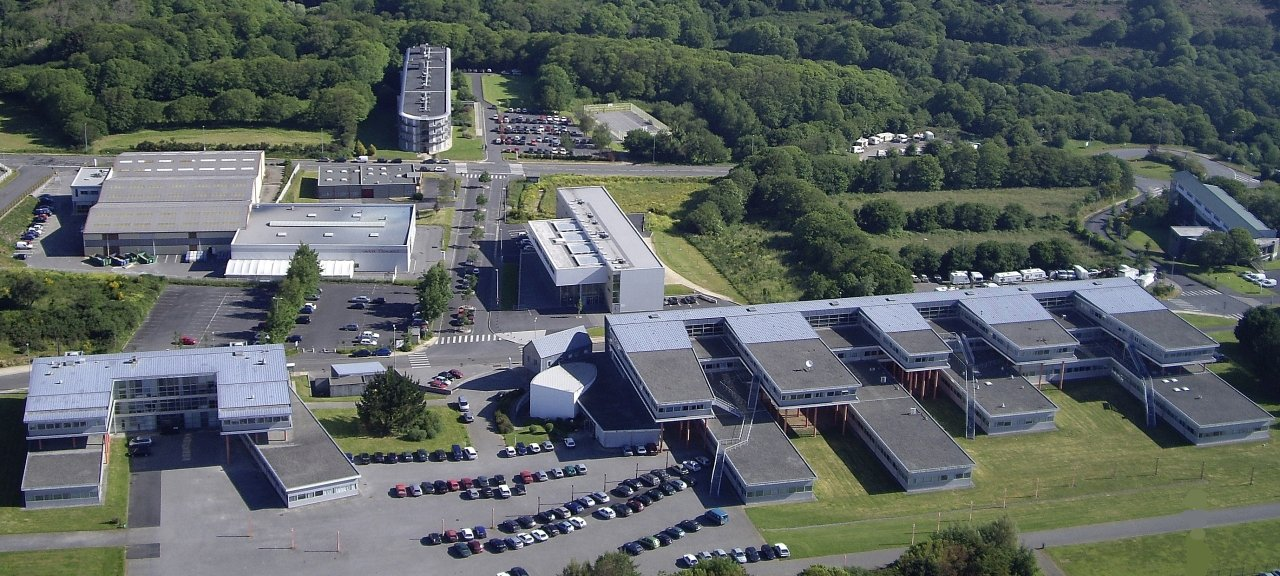
\includegraphics[width=8cm]{enibHaut-1280.jpg}}

\begin{itemize}
\item Au cours des 7 premiers semestres (S1 à S7), les étudiants de l'\enib\ 
suivent les enseignements d'informatique obligatoires 
précisés dans le tableau ci-dessous (660 h).
\end{itemize}

\begin{longtable}{llr}
\hline
Semestre & Thème & Horaires \\
\hline
S1  & Algorithmique                 			& 42 h \\
\hline
S2  & Méthode de développement (projet)     	& 42 h \\
\hline
S3  & Programmation procédurale     			& 73 h \\
\hline
S4  & Programmation orientée objets      		& 42 h \\
\hline
S5  & Langages orientés objets               	& 42 h \\
S5  & Méthodes numériques						& 52 h \\
S5  & Microprocesseurs							& 52 h \\
\hline
S6  & Projet orienté objets			        	& 42 h \\
S6  & Modèles pour l'ingénierie des systèmes 	& 42 h \\
S6  & Bases de données                       	& 21 h\\
S6  & Microprocesseurs							& 42 h \\
\hline
S7	& Systèmes embarqués numériques				& 84 h \\
S7	& Communication réseau et système			& 84 h \\
\hline
%S9	& Projet informatique						& 84 h \\
\end{longtable}

\begin{itemize}
\item Au cours du semestre S7, les étudiants doivent suivre en plus des modules obligatoires
1~module de spécialité au choix (1 $\times$ 84 h).
\item Au cours du semestre S9,
les étudiants doivent suivre 3 modules de spécialité au choix (3~$\times$~84 h)
et un module projet (1 $\times$ 84 h).

Les modules à caractère informatique sont donnés dans le tableau ci-dessous.
\end{itemize}

\begin{longtable}{llr}
\hline
Semestre & Thème & Horaires \\
\hline
S7 ou S9 & Conception d'applications interactives 							& 84 h \\
S7 ou S9 & Méthodologie pour le développement des systèmes d'information 	& 84 h \\
S7 ou S9 & Traitement des signaux et des images 							& 84 h \\
\hline
S9 	& Contrôle-commande 						& 84 h \\
S9 	& Conception des systèmes sur puce 			& 84 h \\
S9 	& Intelligence artificielle et simulation 	& 84 h \\
S9 	& Réalité et environnements virtuels		& 84 h \\
\hline
S9 	& Projet informatique						& 84 h \\
\hline
\end{longtable}

\begin{itemize}
\item Les semestres S8 et S10 sont consacrés à des stages en entreprises. 
\end{itemize}

%-------------------------------------------------------------------------
\subsection*{Recherches en informatique}
%-------------------------------------------------------------------------
La recherche à l'\enib\ est menée au sein de deux unités de recherche :
une dans le domaine des Sciences pour l'ingénieur (\lbms), 
une dans le domaine des Sciences et technologies de l'information et 
de la communication (\labsticc).

\marginpar{
\begin{minipage}{4cm}
	
\includegraphics[height=1cm]{logo-labsticc.png}\hspace*{2mm}
	
\includegraphics[height=1cm]{logo-cnrs.jpg}
\end{minipage} \href{http://www.lab-sticc.fr}{\tt www.lab-sticc.fr}
}
Les enseignants-chercheurs en informatique de l'\enib\ mènent leurs recherches au sein du {\labsticc} 
(Laboratoire des sciences et techniques de l'information, de la communication et de la connaissance),
une Unité mixte de recherche du \cnrs\ (\cnrs\ \umr\ 6285) commune 
à l'\enib, 
à l'Ecole nationale supérieure de techniques avancées de {Bretagne} (\ensta\ \textsc{Bretagne}),
à \tb, 
à l'Université de Bretagne Occidentale (\ubo) et 
à l'Université de Bretagne Sud (\ubs).

\marginpar{
\cerv : \href{http://www.cerv.fr}{\tt www.cerv.fr}\\[1mm]
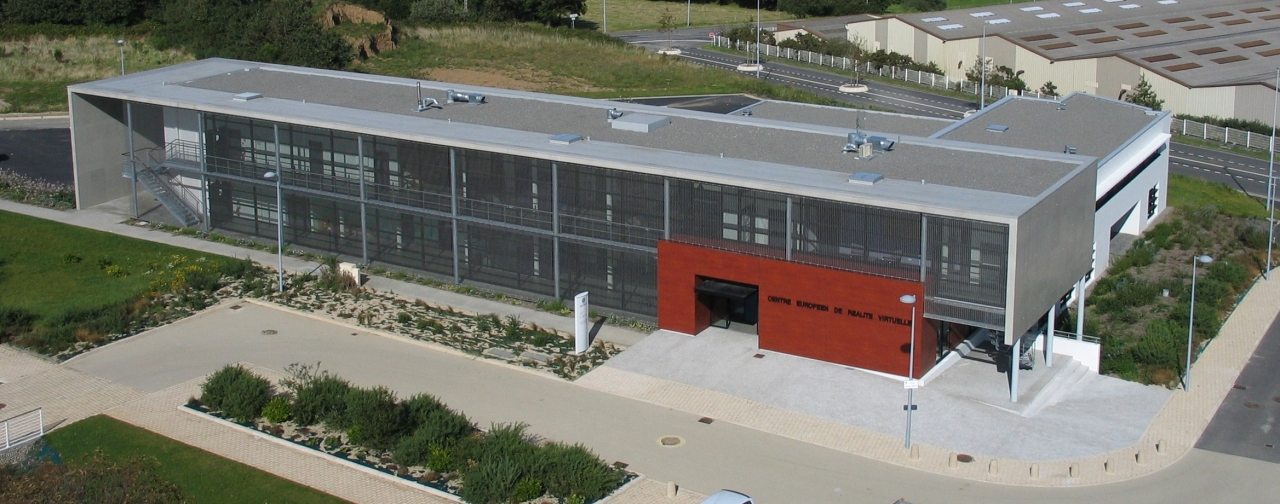
\includegraphics[width=8cm]{cervFacade-1280.jpg}
}
Ils sont installés au Centre européen de réalité virtuelle (\href{http://www.cerv.fr/}{\cerv}), 
établissement de l'\enib\ ouvert en juin 2004, qui accueille des chercheurs 
du \href{http://www.lab-sticc.fr/}{\labsticc}, 
du Centre de recherche sur l’éducation, les apprentissages et la didactique (\href{http://cread.espe-bretagne.fr/}{\cread}) et 
de l'Institut de recherche technologique \bcom\ (\href{http://b-com.com/}{\irt\ \bcom}),
ainsi que les comédiens de la compagnie professionnelle de théâtre \href{http://www.impro-infini.fr/}{Impro-Infini}.




%-------------------------------------------------------------------------
\chapter{Instructions de base}\label{ch:instructions}
%-------------------------------------------------------------------------
	\marginpar{\vspace*{-2cm}\minitoc}
	\noindent\fbox{
\includegraphics[width=0.75\textwidth,page=1]{../../pdf/cours/instructionsSlide.pdf}}
	\newpage
	%-------------------------------------------------------------------------
% info-S1-instructions.tex
%-------------------------------------------------------------------------


%-------------------------------------------------------------------------
\section{Introduction}
%-------------------------------------------------------------------------
Un algorithme est une suite ordonnée d'instructions qui indique la démarche à
suivre pour résoudre une série de problèmes équivalents. Ainsi quand on définit
un algorithme, celui-ci ne doit contenir que des instructions compréhensibles
par celui qui devra l'exécuter. Dans ce cours, nous devrons donc apprendre à
définir des algorithmes pour qu'ils soient compréhensibles --- et donc
exécutables --- par un ordinateur.

%-------------------------------------------------------------------------
\subsection{Jeu d'instructions}
%-------------------------------------------------------------------------
\marginpar{\footnotesize\em
\begin{rem}On distingue classiquement 2 grands types d'architectures de
micro-processeurs :
\begin{itemize}
\item les architectures {\risc} {\em (Reduced Instruction Set Computer)}
	préconisent un petit nombre d'instructions élémentaires dans un format
	fixe;
\item les architectures {\cisc} {\em (Complex Instruction Set Computer)}
	sont basées sur des jeux d'instructions très riches de taille variable
	offrant des instructions composées de plus haut niveau d'abstraction.
\end{itemize}
Chaque architecture possède ses avantages et ses inconvénients :
pour le {\risc} la complexité est reportée au niveau du compilateur,
pour le {\cisc} le décodage est plus pénalisant. 
En fait les machines {\cisc} se sont orientées vers une architecture {\risc} 
où les instructions {\cisc} sont traduites en instructions 
{\risc} traitées par le c\oe ur du processeur. 
\end{rem}}
Chaque microprocesseur a son jeu d'instructions\index{matériel!jeu d'instructions} de base 
dont le nombre varie
typiquement de quelques dizaines à quelques centaines selon le type 
d'architecture du processeur.
On peut classer ces instructions de base en 5 grands groupes :
les opérations arithmétiques ({\tt +}, {\tt -}, {\tt *}, {\tt /}\ldots),
les opérations logiques ({\tt not}, {\tt and}, {\tt or}\ldots),
les instructions de transferts de données ({\tt load}, {\tt store}, {\tt move}\ldots),
les instructions de contrôle du flux d'instructions (branchements impératifs
	et conditionnels, boucles, appels de procédure\ldots),
et les instructions d'entrée-sortie ({\tt read}, {\tt write}\ldots).
\marginpar{\footnotesize\em
\begin{rem}Le c\oe ur du microprocesseur est régulé par un quartz qui 
oscille avec une fréquence exprimée en Hz.
Le temps de cycle est l'inverse de la fréquence.
Ainsi pour une fréquence de 100 MHz, on a un temps de cycle de 10 ns.
L'exécution d'une instruction nécessite plusieurs temps de cycle, 
c'est ce que l'on appelle le {\cpi} {\em(Cycles per Instruction)}\index{matériel!cpi}.
\end{rem}}
Le traitement des ces instructions par le microprocesseur
passe ensuite par 5 étapes :
\begin{enumerate}
\item {\tt fetch} : chargement depuis la mémoire de la prochaine instruction 
	à exécuter,
\item {\tt decode} : décodage de l'instruction,
\item {\tt load operand} : chargement des données nécessaires à l'instruction,
\item {\tt execute} : exécution de l'instruction,
\item {\tt result write back} : mise à jour du résultat dans un registre 
	ou en mémoire.
\end{enumerate}

Le langage machine est le langage compris par le microprocesseur. 
Ce langage est difficile à maîtriser puisque chaque instruction est 
codée par une séquence donnée de bits. Afin de faciliter la tâche 
du programmeur, on a d'abord créé le langage assembleur qui utilise 
des mnémoniques pour le codage des instructions puis les langages de 
plus haut niveau d'expressivité ({\fortran}, {\sc C}, {\java},
{\python}\ldots). Le tableau ci-dessous compare les codes
équivalents pour décrire l'addition de 2 entiers dans différents langages
informatiques : le langage machine, le langage assembleur, le langage {\pascal} 
et le langage {\python}. On constate sur cet exemple
une évolution progressive du pouvoir d'expressivité des langages,
du langage machine aux langages de haut niveau.
$$\begin{tabular}{|l|l|l|l|}
\hline
machine & assembleur & {\pascal} & {\python} \\
\hline
\begin{minipage}{2.5cm}\footnotesize\tt
A1 00 01\\
8B 1E 02 01\\
01 D8\\
A3 04 01
\end{minipage} &	
\begin{minipage}{2.5cm}\footnotesize\tt
MOV AX,[100h]\\
MOV BX,[102h]\\
ADD AX,BX\\
MOV [104h],AX 	
\end{minipage} &	
\begin{minipage}{3.5cm}\footnotesize\tt
var a,b,c : integer;\\
c := a + b;
\end{minipage} &	
\begin{minipage}{2.5cm}\footnotesize\tt
c = a + b
\end{minipage} \\
\hline
\end{tabular}$$


%-------------------------------------------------------------------------
\subsection{Instructions de base}
%-------------------------------------------------------------------------
Dans ce cours, nous nous intéresserons aux instructions disponibles
dans un langage de haut niveau tel que {\python}.
\marginpar{\footnotesize\em 
\begin{minipage}{4cm}
\includegraphics[width=4cm]{python-logo.jpg}\end{minipage}\hfill
\href{http://www.python.org}{\tt www.python.org}}
Les principales instructions ({\em statements}) concerneront 
l'affectation ({\em assignment}), 
les tests ({\em conditional statements})
et les boucles ({\em loops}).
Le tableau ci-dessous donne la syntaxe {\sc Python} des instructions de base
qui seront utilisées dans ce chapitre (d'après \cite{gruet}). Une liste plus détaillée des principales 
instructions en {\python} est proposée en annexe \ref{python} page \pageref{python}.

\marginpar{\footnotesize\em
\begin{rem} L'anglais est la langue couramment utilisée en informatique.
Il est absolument essentiel de lire l'anglais technique sans problème.
Vous devez être capable de traduire le tableau ci-contre extrait sans
traduction d'une référence en anglais \cite{gruet}.
\end{rem}
}
\index{langage!{{\python}}!instructions}\label{cite:gruet1}
$$\begin{tabular}{|p{5.5cm}|p{9cm}|}
\hline
\bf Statement & \bf Result \\
\hline
\tt pass & Null statement \\
\hline
\tt print([s1] [, s2 ]*) & Writes to {\tt sys.stdout}. 
                              Puts spaces between arguments {\tt si}. Puts newline at end unless arguments end with {\tt end=} (ie: {\tt end=' '}).
		              {\tt print} is not required when running interactively, simply typing an expression will print its value, 
		              unless the value is {\tt None}.\\
\hline
\tt a = b 	  & Basic assignment - assign object {\tt b} to label {\tt a}\\
\hline
\tt if condition:\newline
\mbox{}\ \ suite\newline
[elif condition: suite]*\newline
[else:\newline
\mbox{}\ \ suite] & Usual {\tt if/else if/else} statement.\\
\hline
\tt while condition:\newline
\mbox{}\ \ suite  & Usual {\tt while} statement. \\
\hline
\tt for element in sequence:\newline
\mbox{}\ \ suite  & Iterates over {\tt sequence}, assigning each element to {\tt element}. 
           Use built-in {\tt range} function to iterate a number of times.\\
\hline
\end{tabular}$$


%-------------------------------------------------------------------------
\section{Affectation}\label{affectation}
%-------------------------------------------------------------------------

%-------------------------------------------------------------------------
\subsection{Variables}\label{sub:variables}
%-------------------------------------------------------------------------
\begin{ex}[La température Fahrenheit]\mbox{}
Le degré Fahrenheit ($\,^\circ F$) est une unité de mesure de la température, 
qui doit son nom au physicien allemand Daniel Gabriel Fahrenheit (1686-1736), qui la proposa 
en 1724. Dans l'échelle de température de Fahrenheit, le point de solidification 
de l'eau est de 32 degrés, et son point d'ébullition de 212 degrés. Ainsi par exemple, 
$70^\circ F$ correspondent approximativement à $21^\circ C$.
\end{ex}
\marginpar{\em\footnotesize
\begin{td}[Unité de pression]\label{td:torr}\index[td]{unité de pression}
Le torr (torr) ou millimètre de mercure (mmHg) est une unité de mesure 
de la pression qui tire son nom du physicien et mathématicien italien Evangelista Torricelli (1608-1647).
Il est défini comme la pression exercée à 0°C par une colonne de 1 millimètre de mercure (mmHg).
Il a plus tard été indexée sur la pression atmosphérique : 1 atmosphère normale correspond à 
760 mmHg et a 101 325 Pa.

Ecrire une instruction qui permette de passer directement des torrs au pascals (Pa).
\end{td}}

\noindent Pour effectuer la conversion Fahrenheit $\rightarrow$ Celcius, nous commençons par donner un
nom à la température Fahrenheit, par exemple {$t_F$}, ainsi qu'à la température Celcius,
par exemple {$t_C$}. Puis nous pouvons exprimer la relation générale qui lie {$t_C$} à {$t_F$} :
{$\displaystyle t_C = \frac{5}{9}(t_F - 32)$} et appliquer cette relation
dans un cas particulier, par exemple $t_F = 70$ : $\displaystyle t_C = \frac{5}{9}(70 - 32) \approx 21$.
\exo{td:torr}
\marginpar{\em\footnotesize
\begin{fig}[Définition de l'académie (4)]\label{fig:dico4}
{\bf DÉNOTER} v. tr. XIVe siècle. Emprunté du latin denotare, « désigner, faire connaître ».
1. Indiquer comme caractéristique, signifier, révéler. 2. LOGIQUE. Désigner 
la totalité des objets dont les caractères sont fixés par un concept. 
\end{fig}

\begin{rem}Une variable peut être vue comme une case en mémoire vive, que le programme 
va repérer par une étiquette (une adresse ou un nom). Pour avoir accès au contenu de la case
(la valeur de la variable), il suffit de la désigner par son étiquette : c'est-à-dire 
soit par son adresse en mémoire, soit par son nom.
\end{rem}
}

En informatique, l'essentiel du travail effectué par un programme d'ordinateur consiste 
à manipuler des données. Ces données peuvent être très diverses (par exemple des températures) et
pour accéder à ces données, il est pratique de les nommer plutôt que de connaître
explicitement leur adresse en mémoire. 

Une donnée apparaît ainsi sous un nom de variable (par exemple {\tt tC} ou {\tt tF}) :
on dit que la variable dénote une valeur (figure \ref{fig:dico4}).
Pour la machine, il s'agit d'une référence 
désignant une adresse mémoire, c'est-à-dire un emplacement précis dans la mémoire vive où est
stockée une valeur bien déterminée qui est la donnée proprement dite.

\begin{defin}[variable]\index[def]{variable}\index{variable!définition}
Une variable est un objet informatique qui associe un nom à une valeur 
qui peut éventuellement varier au cours du temps.
\end{defin}

Les noms de variables sont des identificateurs arbitraires, de préférence assez courts mais aussi 
explicites que possible, de manière à exprimer clairement ce que la variable est censée 
référencer (la sémantique de la donnée référencée par la variable). 
Les noms des variables\index{variable!nom de variable} doivent en outre obéir à quelques règles simples :
\marginpar{\em\footnotesize
\begin{rem}En mathématiques, une « variable » est généralement une inconnue, 
qui recouvre un nombre non précisé de valeurs.
En informatique, une variable possède à un moment donné une valeur et une seule.
\end{rem}

\begin{fig}[Mots réservés en {\sc Python}]\label{fig:motscles}\tt\mbox{}\\
\centerline{\begin{tabular}{lllll}
        and       & del       & for       & is        & raise \\
        assert    & elif      & from      & lambda    & return\\
        break     & else      & global    & not       & try\\
        class     & except    & if        & or        & while\\
        continue  & exec      & import    & pass      & with\\
        def       & finally   & in        & print     & yield
\end{tabular}}
\end{fig}}
\begin{itemize}
\item Un nom de variable est une séquence de lettres (a\ldots  z , A\ldots  Z) et de chiffres (0\ldots  9), qui
      	doit toujours commencer par une lettre.
\item Seules les lettres ordinaires sont autorisées. Les lettres accentuées, les cédilles, les espaces, les
      	caractères spéciaux tels que {\tt \$}, {\tt \#}, {\tt @}, etc. sont interdits, 
      	à l'exception du caractère {\tt \_} (souligné).
\item La « casse » est significative : les caractères majuscules et minuscules sont distingués. Ainsi,
      	{\tt python}, {\tt Python}, {\tt PYTHON} sont des variables différentes. 
\item Par convention, on écrira l'essentiel des noms de variable en caractères minuscules (y compris la
	première lettre). On n'utilisera les majuscules qu'à l'intérieur même du nom  
	pour en augmenter éventuellement la lisibilité, comme dans {\tt programmePython} ou
	{\tt angleRotation}.
	Une variable dont la valeur associée ne varie pas au cours du programme (on parle alors de constante)
	pourra être écrite entièrement en majuscule, par exemple {\tt PI} ($\pi = 3.14$).
\item Le langage lui-même peut se réserver quelques noms comme c'est le cas pour {\sc Python} 
	(figure \ref{fig:motscles}). Ces mots réservés ne peuvent donc pas être
	utilisés comme noms de variable.\index{langage!{{\sc Python}}!mots réservés}
\end{itemize}


%-------------------------------------------------------------------------
\subsection{Attribuer une valeur}
%-------------------------------------------------------------------------
Une fois nommée, il est souvent nécessaire de modifier la valeur de la donnée
référencée par une variable. C'est le rôle de l'instruction d'affectation.
\index{instruction!affectation}
\marginpar{\footnotesize\em
\begin{fig}[Types de base en \python]\label{fig:types}\mbox{}\\
\centerline{\begin{tabular}{lll}
type & nom & exemples \\
\hline
booléens & \tt bool & {\tt False}, {\tt True}\\
entiers  & \tt int  & \tt 3, -7\\
réels    & \tt float & \tt 3.14, 7.43e-3\\
chaînes  & \tt str & \tt 'salut', "l'eau"\\
n-uplets & \tt tuple & \tt 1,2,3\\
listes   & \tt list  & \tt [1,2,3] \\
dictionnaires & \tt dict & \tt \{'a':4, 'r':8\}
\end{tabular}}
\end{fig}}

\begin{defin}[affectation]\label{def:affectation}\index[def]{affectation}\index{affectation}
L'affectation est l'opération qui consiste à attribuer une valeur à une variable.
\end{defin}

L'instruction d'affectation est notée {\tt =} en {\sc Python} : \fbox{\tt variable = valeur}. 
Le nom de la variable à modifier est placé dans le membre de gauche du signe {\tt =}, 
la valeur qu'on veut lui attribuer dans le membre de droite. 
Le membre de droite de l'affectation est d'abord évalué sans être modifié
puis la valeur obtenue est affectée à la variable dont le nom est donné dans 
le membre de gauche de l'affectation; ainsi, cette opération ne modifie 
que le membre de gauche de l'affectation.
Le membre de droite peut être une constante ou une expression évaluable.


\begin{description}
\item[\fbox{\tt variable = constante}] : La constante peut être d'un type quelconque (figure \ref{fig:types}) :
	entier, réel, booléen, chaîne de caractères, tableau, matrice, dictionnaire\ldots\ comme le suggèrent
	les exemples suivants :

	\mbox{}\hfill
	\begin{minipage}[t]{4.5cm}
	\begin{verbatim}
	booleen = False
	entier = 3
	reel = 0.0
	chaine = "salut"
	tableau = [5,2,9,3]
	matrice = [[1,2],[6,7]]
	nUplet = 4,5,6
	dictionnaire = {}
	\end{verbatim}
	\end{minipage}
	\hfill
	\begin{minipage}[t]{9cm}
	\begin{verbatim}
	autreBooleen = True
	autreEntier = -329
	autreReel = -5.4687e-2
	autreChaine = 'bonjour, comment ça va ?'
	autreTableau = ['a',[6,3.14],[x,y,[z,t]]]
	autreMatrice = [[1,2],[3,4],[5,6],[7,8]]
	autreNUplet = "e",True,6.7,3,"z"
	autreDictionnaire = {"a":7, "r":-8}
	\end{verbatim}
	\end{minipage}
	
\item[\fbox{\tt variable = expression}] : L'expression peut être n'importe quelle expression évaluable
	telle qu'une opération logique ({\tt x = True or False and not True}), une opération
	arithméti\-que ({\tt x = 3 + 2*9 - 6*7}), un appel de fonction ({\tt y = sin(x)}) ou toute 
	autre combinaison évaluable
	({\tt x = (x != y) and (z + t >= y) or (sin(x) < 0)}).
	\exo{td:suiteArit}

	\mbox{}\hfill
	\begin{minipage}[t]{4cm}
	\begin{verbatim}
	reste = a%b
	somme = n*(n+1)/2
	delta = b*b - 4*a*c
	surface = pi*r**2
	\end{verbatim}
	\end{minipage}
	\hfill
	\begin{minipage}[t]{9.5cm}
	\begin{verbatim}
	quotient = a/b
	sommeGeometrique =  s = a*(b**(n+1) - 1)/(b-1)
	racine = (-b + sqrt(delta))/(2*a)
	volume = surface * hauteur
	\end{verbatim}
	\end{minipage}

	L'expression du membre de droite peut faire intervenir la variable 
	du membre de gauche comme dans {\tt i = i + 1}. Dans cet exemple, on évalue
	d'abord le membre de droite ({\tt i + 1}) puis on attribue la valeur obtenue au
	membre de gauche ({\tt i}); ainsi, à la fin de cette affectation, la valeur de {\tt i}
	a été augmentée de {\tt 1} : on dit que {\tt i} a été incrémenté de {\tt 1}
	(figure \ref{fig:dico5}) et on parle d'incrémentation de la variable {\tt i}
	(remarque \ref{rem:affectation}). \python\ propose un opérateur d'incrémentation ({\tt +=})
	et d'autres opérateurs d'affectation qui peuvent toujours se ramener
	à l'utilisation de l'opérateur {\tt =}, l'opérateur d'affectation de base 
	(figure \ref{fig:affectations}).
\end{description}

	\marginpar{\em\footnotesize\vspace*{-14cm}
	\begin{td}[Suite arithmétique (1)]\label{td:suiteArit}\index[td]{suite arithmétique}
	Ecrire une instruction qui calcule la somme $s = \sum_0^n u_k$ des $n$ premiers 
	termes d'une suite arithmétique $u_k = a + r\cdot k$. 
	\end{td}

	\begin{fig}[Définition de l'académie (5)]\label{fig:dico5}
	{\bf INCRÉMENT} n. m. XVe siècle, encrement. Emprunté du latin incrementum, « accroissement ».
	INFORM. Quantité fixe dont on augmente la valeur d'une variable à chaque phase de l'exécution du programme.\\
	{\bf DÉCRÉMENT} n. m. XIXe siècle. Emprunté de l'anglais decrement, du latin decrementum, 
	« amoindrissement, diminPrincipales affectations en {\sc Python}ution ». 
	MATH. INFORM. Quantité fixe dont une grandeur diminue à chaque cycle.
	\end{fig}

	\begin{rem}\label{rem:affectation}
	Avec l'exemple de l'incrémentation ({\tt i = i + 1}), 
	on constate que l'affectation est une opération 
	typiquement informatique qui se distingue de l'égalité mathématique. En effet,
	en mathématique une expression du type {\tt i = i+1} se réduit en
	{\tt 0 = 1} ! Alors qu'en informatique, l'expression {\tt i = i+1} conduit à ajouter {\tt 1} 
	à la valeur de {\tt i} (évaluation de l'expression {\tt i+1}), puis à donner cette
	nouvelle valeur à {\tt i} (affectation).
	\end{rem}

	\begin{fig}[Principales affectations en {\sc Python}]\label{fig:affectations}\tt\mbox{}\\
	\centerline{\tt\begin{tabular}{lll}
	a = b  & & \\ 
	\hline	
	a += b & $\equiv$ & a = a + b \\
	a -= b & $\equiv$ & a = a - b \\	
	a *= b & $\equiv$ & a = a * b \\ 	
	a /= b & $\equiv$ & a = a / b \\ 	
	a \%= b & $\equiv$ & a = a \% b \\	
	a **= b& $\equiv$ & a = a ** b 	
	\end{tabular}}
	\end{fig}
	}
	
L'affectation a ainsi pour effet de réaliser plusieurs opérations dans la mémoire de l'ordinateur :
\begin{itemize}
\item créer et mémoriser un nom de variable,
\item lui attribuer un type bien déterminé,
\item créer et mémoriser une valeur particulière,
\item établir un lien (par un système interne de pointeurs) entre le nom de la variable 
	et l'emplacement mémoire de la valeur correspondante.
\end{itemize}


%-------------------------------------------------------------------------
\subsection{Séquences d'affectations}
%-------------------------------------------------------------------------
\begin{ex}[Permutation de 2 nombres]\label{ex:swap}\index[algo]{permutation de nombres}
Un apprenti informaticien a qui on demandait d'échanger ({\em swap}) les valeurs
de 2 variables {\tt x} et {\tt y} proposa la suite d'instructions suivante :\\
{\footnotesize\tt
\mbox{}\ \ x = y\\
\mbox{}\ \ y = x\\}
et eut la désagréable surprise de constater que les valeurs des variables 
n'étaient pas permutées après cette séquence d'affectations.
\end{ex}
\marginpar{\footnotesize\em
	\begin{rem}
	L'affectation n'est pas une opération commutative (symétrique) : {\tt a = b} $\neq$ {\tt b = a}. 
	En effet, avec l'instruction {\tt a = b}
	on modifie la valeur de {\tt a} et pas celle de {\tt b} tandis qu'avec l'instruction
	{\tt b = a}, on modifie {\tt b} mais pas {\tt a}.
	\end{rem}}
\noindent En effet, pour fixer les idées supposons qu'initialement {\tt x = 10} et {\tt y = 20}.
L'affectation {\tt x = y} conduit à évaluer {\tt y} puis à attribuer la valeur de {\tt y} ({\tt 20})
à {\tt x} : {\tt x} vaut maintenant {\tt 20}. La deuxième affectation ({\tt y = x}) 
commence par évaluer {\tt x} puis à attribuer la valeur de {\tt x} ({\tt 20} !) à {\tt y}.
Après ces 2 affectations, {\tt x} et {\tt y} sont donc identiques et non permutées! 
Pour effectuer la permutation, l'apprenti informaticien aurait pu utiliser une variable 
temporaire (que nous nommerons {\tt tmp}) et exécuter la séquence d'instructions suivante :\\
\begin{minipage}[t]{2cm}\footnotesize\tt
\mbox{}\ \ tmp = x\\
\mbox{}\ \ x = y\\
\mbox{}\ \ y = tmp
\end{minipage}
\marginpar{\em\footnotesize
\begin{rem} En \python, les n-uplets permettent d'écrire plus simplement la permutation
de variables :\\\tt
\mbox{}\ \ x, y = y, x
\end{rem}

\begin{td}[Permutation circulaire (1)]\label{td:permutation1}\index[td]{permutation circulaire}
Effectuer une permutation circulaire droite entre les valeurs de 4 entiers $x$, $y$, $z$ et $t$.
\end{td}
}
\hfill
\begin{minipage}[t]{13cm}\footnotesize
La première affectation ({\tt tmp = x}) permet de stocker la valeur initiale de {\tt x} ({\tt 10}),
la deuxième ({\tt x = y}) attribue à {\tt x} la valeur de {\tt y} ({\tt 20}) et la troisième ({\tt y = tmp})
attribue à {\tt y} la valeur de {\tt tmp}, c'est-à-dire la valeur initiale de {\tt x} ({\tt 10}).
Ainsi, les valeurs finales de {\tt x} et {\tt y} ({\tt 20} et {\tt 10}) sont bien permutées 
par rapport aux valeurs initiales ({\tt 10} et {\tt 20}).
\end{minipage}

\mbox{}\exo{td:permutation1}

\begin{ex}[Un calcul de pgcd (1)]\label{ex:pgcd1}\index[algo]{algorithme d'{{\sc Euclide}}}
Le plus grand commun diviseur de 2 entiers $a$ et $b$ peut se calculer en appliquant
la relation de récurrence ${\rm pgcd}(a,b) = {\rm pgcd}(b,a\mbox{\tt\%}b)\mbox{ si } b \neq 0$ 
jusqu'à ce que le reste ($a\%b$) soit nul (${\rm pgcd}(d,0) = d\mbox{ si } d \neq 0$).
\end{ex}
\noindent Ainsi, pour calculer le pgcd de $a=12$ et de $b=18$, on applique 3 fois de suite
cette relation :
${\rm pgcd}(a,b) = {\rm pgcd}(b,a\mbox{\tt\%}b) \Rightarrow {\rm pgcd}(12,18) = 
{\rm pgcd}(18,12) = {\rm pgcd}(12,6) = {\rm pgcd}(6,0) = 6$. 
Ce qui peut se traduire en \python\ par la séquence d'affectations suivante :\\
	\noindent{\footnotesize\tt\mbox{}\ \ \begin{tabular}[t]{l@{\hspace*{1cm}\# }l}
	a = 12 & $a=12$\\
	b = 18 & $b=18$\\
	r = a\%b & $r=12$\\
	a = b & $a=18$\\
	b = r & $b=12$\\
	r = a\%b & $r=6$
	\end{tabular}\hspace*{1cm}
	\begin{tabular}[t]{l@{\hspace*{1cm}\# }l}
	a = b & $a=12$\\
	b = r & $b=6$\\
	r = a\%b & $r=0$\\
	a = b & $a=6$\\
	b = r & $b=0$
	\end{tabular}}\\
A la fin de la séquence, on a $a=6$ et $b=0$ : $a$ est le pgcd recherché.
\exo{td:seq1}
\marginpar{\footnotesize\em\vspace*{-3cm}
\begin{td}[Séquence d'affectations (1)]\label{td:seq1}\index[td]{séquence d'affectations}
Quelles sont les valeurs des variables $a$, $b$, $q$ et $r$ 
après la séquence d'affectations suivante ?
	
	\noindent{\footnotesize\tt
	\mbox{}\ \ a = 19\\
	\mbox{}\ \ b = 6\\
	\mbox{}\ \ q = 0\\
	\mbox{}\ \ r = a\\
	\mbox{}\ \ r = r - b\\
	\mbox{}\ \ q = q + 1\\
	\mbox{}\ \ r = r - b\\
	\mbox{}\ \ q = q + 1\\
	\mbox{}\ \ r = r - b\\
	\mbox{}\ \ q = q + 1
	}
\end{td}
}

Les 2 exemples \ref{ex:swap} et \ref{ex:pgcd1} précédents illustrent la possibilité
de réaliser des calculs plus ou moins compliqués à l'aide d'une séquence d'affectations 
bien choisies. Mais ce sont les tests et les boucles qui nous permettront
d'aborder des algorithmes réutilisables, et plus robustes, en améliorant
l'expressivité du programmeur.


%-------------------------------------------------------------------------
\section{Tests}\label{tests}
%-------------------------------------------------------------------------
\marginpar{\footnotesize\em
\begin{fig}[Flux d'instructions]\label{fig:flux}\mbox{}\\
\centerline{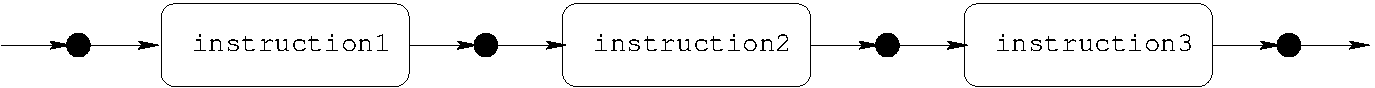
\includegraphics[width=7.5cm]{uml0.pdf}}
\end{fig}

\begin{fig}[Définition de l'académie (6)]\label{fig:dico6}
\mbox{}\\
{\bf ALTERNATIVE} n. f. XVe siècle, comme terme de droit ecclésiastique ; 
XVIIe siècle, au sens moderne. Forme féminine substantivée d'alternatif.
Choix nécessaire entre deux propositions, deux attitudes dont l'une exclut l'autre. 
\end{fig}}
Sauf mention explicite, les instructions d'un algorithme s'exécutent 
les unes après les autres, dans l'ordre où elles ont été écrites.
Le « chemin » suivi à travers un algorithme est appelé le flux d'instructions
(figure \ref{fig:flux}), 
et les constructions qui le modifient sont appelées des instructions de contrôle de flux.
On exécute normalement les instructions de la première à la dernière, sauf lorsqu'on rencontre
une instruction de contrôle de flux : de telles instructions vont permettre de suivre 
différents chemins suivant les circonstances.
C'est en particulier le cas de l'instruction conditionnelle qui n'exécute une instruction
que sous certaines conditions préalables. Nous distinguerons ici 3 variantes d'instructions conditionnelles 
(figure \ref{fig:dico6}) : 
\marginpar{\footnotesize\em
\begin{rem}A propos des instructions conditionnelles, on parle souvent des instructions 
« {\tt if} » dans le jargon des informaticiens.
\end{rem}

\begin{rem}{\tt elif ...} et la contraction de {\tt else: if ...}.\end{rem}
}
\index{test}\index{alternative|see{test}}
$$\begin{tabular}{|l|l|}
\hline
\multicolumn{2}{|c|}{Instructions conditionnelles}\\
\hline
test simple         & {\begin{minipage}[t]{6cm}\tt if condition : blocIf \\ \mbox{} \end{minipage}} \\
\hline
alternative simple   & {\begin{minipage}[t]{6cm}\tt if condition : blocIf\\else: blocElse \\ \mbox{} \end{minipage}} \\
\hline
alternative multiple & {\begin{minipage}[t]{6cm}\tt if condition : blocIf\\elif condition1: blocElif1\\elif
condition2: blocElif2\\ \ldots \\else: blocElse \\ \mbox{} \end{minipage}}\\
\hline
\end{tabular}$$
où {\tt if}, {\tt else} et {\tt elif} sont des mots réservés, {\tt condition} une expression
booléenne (à valeur {\tt True} ou {\tt False}) et {\tt bloc...} un bloc d'instructions.


%-------------------------------------------------------------------------
\subsection{Tests simples}\label{sub:cond}
%-------------------------------------------------------------------------
L'instruction « {\tt if} » sous sa forme la plus simple (figure \ref{fig:test})
permet de tester la validité d'une condition.
\index{instruction!test simple}\index{if1@{{\tt if}}}
Si la condition est vraie,
alors le bloc d'instructions {\tt blocIf} après le « {\tt :} » est exécuté. 
Si la condition est fausse, on passe à l'instruction suivante dans le flux 
d'instructions. 
\marginpar{\footnotesize\em\vspace*{-2cm}
\begin{fig}[Le test simple]\label{fig:test}\tt 
if condition : blocIf
\end{fig}
\index{langage!{{\sc Python}}!opérateurs}
\begin{fig}[Principaux opérateurs \python]\label{fig:operateur}
\begin{description}
\item[Opérateurs logiques :] {\tt not a}, {\tt a and b}, {\tt a or b}
\item[Opérateurs de comparaison :] {\tt x == y}, {\tt x != y},\\{\tt x < y}, {\tt x <= y}, 
	{\tt x > y}, {\tt x >= y}
\item[Opérateurs arithmétiques :] {\tt +x}, {\tt -x}, {\tt x + y}, \\{\tt x - y}, {\tt x * y}, 
	{\tt x / y}, {\tt x \% y}, {\tt x**y}
\end{description}
\end{fig}
\begin{td}[Opérateurs booléens dérivés (1)]\label{td:booleens1}\index[td]{opérateurs booléens dérivés}
En utilisant les opérateurs booléens de base ({\tt not}, {\tt and} et {\tt or}),
écrire un algorithme qui affecte successivement à une variable {\tt s} 
le résultat des opérations booléennes suivantes :
ou exclusif ({\em xor}, $a \oplus b$), 
non ou ({\em nor}, $\overline{a+b}$), 
non et ({\em nand}, $\overline{a\cdot b}$), 
implication ($a \Rightarrow b$) et  
équivalence ($a \Leftrightarrow b$).
\end{td}

\index[algo]{circuits logiques}
\begin{td}[Circuit logique (1)]\label{td:circuits}\index[td]{circuits logiques}
Donner les séquences d'affectations permettant de calculer la sortie $s$
du circuit logique suivant en fonction de ses entrées $a$, $b$ et $c$.
$$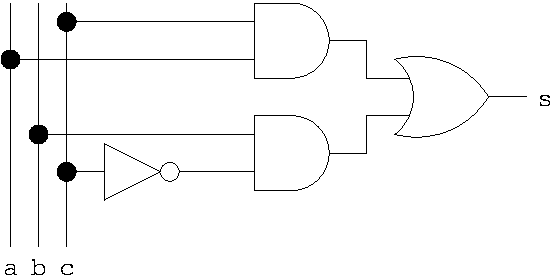
\includegraphics[width=5cm]{mux1.pdf}$$
\end{td}}

\begin{defin}[test simple]\index[def]{test simple}\index{test!test simple}
Le test simple est une instruction de contrôle du flux d'instructions 
qui permet d'exécuter une instruction sous condition préalable.
\end{defin}

La condition évaluée après l'instruction « {\tt if} »  est donc une 
expression booléenne qui prend soit la valeur {\tt False} (faux) soit la valeur 
{\tt True} (vrai). Elle peut contenir les opérateurs de comparaison suivants :
$$\begin{tabular}{l@{\tt\hspace*{1cm}\# }l}
\tt x == y                &  {\tt x} est   égal à {\tt y} \\
\tt x != y                &  {\tt x} est   différent de {\tt y} \\
\tt x > y                 &  {\tt x} est   plus grand que {\tt y} \\
\tt x < y                 &  {\tt x} est   plus petit que {\tt y} \\
\tt x >= y                &  {\tt x} est   plus grand que, ou égal à {\tt y} \\
\tt x <= y                &  {\tt x} est   plus petit que, ou égal à {\tt y}
\end{tabular}$$
Mais certains problèmes exigent parfois de formuler des conditions qui ne peuvent pas être exprimées 
sous la forme d'une simple comparaison. Par exemple, la condition $x \in [0,1[$ s'exprime 
par la combinaison de deux conditions $x \geq 0$ et $x < 1$ qui doivent être vérifiées en même temps. 
Pour combiner ces conditions, on utilise les opérateurs logiques {\tt not}, {\tt and} et {\tt or}
(figure \ref{fig:operateur}). Ainsi la condition $x \in [0,1[$ pourra s'écrire en \python\ :
{\tt (x >= 0) and (x < 1)}.
\exo{td:booleens1}

Le tableau ci-dessous donne les tables de vérité des opérateurs {\tt not}, {\tt or} et {\tt and},
leur représenta\-tion graphique traditionnelle ainsi que leurs principales propriétés. 
\exo{td:circuits}

\index{opérateurs booléens}
$$\begin{tabular}{|c|c|c|}
\hline
négation & disjonction & conjonction \\
\hline
\tt not a & \tt a or b & \tt a and b\\
$\begin{array}{|c|c|}
\hline
a & {\overline{a}}\\
\hline
0 & 1\\
1 & 0\\
\hline
\end{array}$ &
$\begin{array}{|c|c|c|}
\hline
a & b & {a+b}\\
\hline
0 & 0 & 0\\
0 & 1 & 1\\
1 & 0 & 1\\
1 & 1 & 1\\
\hline
\end{array}$ &
$\begin{array}{|c|c|c|}
\hline
a & b & {a\cdot b}\\
\hline
0 & 0 & 0\\
0 & 1 & 0\\
1 & 0 & 0\\
1 & 1 & 1\\
\hline
\end{array}$ \\
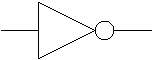
\includegraphics[height=0.75cm]{non.pdf} & 
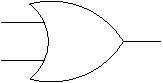
\includegraphics[height=0.75cm]{ou.pdf}  &
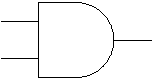
\includegraphics[height=0.75cm]{et.pdf}  \\
\hline
 & \tt not (a or b) & \tt not (a and b) \\
 & 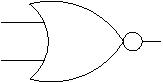
\includegraphics[height=0.75cm]{nonOu.pdf} & 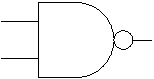
\includegraphics[height=0.75cm]{nonEt.pdf}\\
\hline
\end{tabular}
\hfill
\begin{tabular}{ll}
\multicolumn{2}{l}{$\forall a, b, c \in \{0;1\}$ :}\\
\makebox[0.5cm]{} & {$a + 0 = a$} \hspace*{5mm} {$a \cdot 1 = a$}\\
 & {$a + 1 = 1$} \hspace*{5mm} {$a \cdot 0 = 0$}\\
 & {$a + a = a$} \hspace*{5mm} {$a \cdot a = a$}\\
 & {$a + \overline{a} = 1$} \hspace*{5mm} {$a \cdot \overline{a} = 0$}\\
 & {$a + (a \cdot b) = a$} \hspace*{5mm} {$a \cdot (a + b) = a$}\\
 & {$\overline{\overline{a}}  = a$} \hspace*{5mm} $\overline{a + b} = \overline{a} \cdot \overline{b}$ \hspace*{5mm} $\overline{a\cdot b} = \overline{a} + \overline{b}$\\
 & {$(a+b) = (b+a)$} \hspace*{5mm}  {$(a \cdot b) = (b \cdot a)$} \\
 & {$(a+b)+c = a+(b+c)$} \\ 
 & {$(a\cdot b)\cdot c = a\cdot (b\cdot c)$} \\
 & {$a + (b \cdot c) = (a+b) \cdot (a+c)$} \\ 
 & {$a \cdot (b+ c) = (a \cdot b)+(a\cdot c)$} 
\end{tabular}$$
\exo{td:prop}
\marginpar{\footnotesize\em
\begin{td}[Lois de De Morgan]\label{td:prop}\index{{{\sc De Morgan}}}\index[td]{lois de {{\sc De Morgan}}}
Démontrer à l'aide des tables de vérité les lois de De Morgan 
$\forall a, b \in \{0;1\}$ :
\begin{enumerate}
\item {$\overline{(a+b)} = \overline{a} \cdot \overline{b}$} 
\item {$\overline{(a \cdot b)} = \overline{a} + \overline{b}$}
\end{enumerate}
\end{td}
\begin{fig}[L'alternative simple]\label{fig:alternative}\tt 
if condition : blocIf\\
else: blocElse
\end{fig}

\begin{rem}Le test simple (figure \ref{fig:test} page \pageref{fig:test}) est équivalent 
à une alternative simple où on explicite le fait de ne rien faire (instruction {\tt pass})
dans le bloc d'instructions associé au {\tt else}:\\
{\tt
\mbox{}\ \ if condition : bloc\\
\mbox{}\ \ else: pass}\\
\mbox{}\hfill voir également le TD \ref{td:reciproque} page \pageref{td:reciproque}.
\end{rem}}

%-------------------------------------------------------------------------
\subsection{Alternatives simples}\label{sub:alternative}
%-------------------------------------------------------------------------
\begin{ex}[Extrait d'un dialogue entre un conducteur égaré et un piéton]\label{ex:chemin}
\begin{itemize}
\item Pourriez-vous m'indiquer le chemin de la gare, s'il vous plait ?
\item Oui bien sûr : vous allez tout droit jusqu'au prochain carrefour.
	Si la rue à droite est autorisée à la circulation --- hier elle était en travaux --- 
	alors prenez la et ensuite c'est
	la deuxième à gauche et vous verrez la gare. Sinon, au carrefour, vous allez tout droit 
	et vous prenez la
	première à droite, puis encore la première à droite et vous y êtes.
\item Merci.
\end{itemize}
\end{ex}
\noindent L'algorithme décrit par le piéton propose une alternative entre deux solutions.
Le conducteur égaré devra tester si la rue est en travaux avant de prendre la décision 
d'aller à droite au carrefour ou de continuer tout droit. En algorithmique, un tel
choix est proposé par l'alternative simple, instruction conditionnelle
dite « {\tt if} \ldots\ {\tt else} ».\index{if2@{{\tt if\ \ldots\ else}}}

L'instruction « {\tt if} \ldots\ {\tt else} » teste une condition (figure \ref{fig:alternative}). 
\index{instruction!alternative simple}
Si la condition
est vraie, alors le bloc d'instructions {\tt blocIf} après le « {\tt :} » est exécuté.
Si la condition est fausse, c'est le bloc d'instructions {\tt blocElse} après le « {\tt else:} » 
(sinon) qui est exécuté. Seul l'un des 2 blocs est donc exécuté.

\begin{defin}[alternative simple]\index[def]{alternative simple}\index{test!alternative simple}
L'alternative simple est une instruction de contrôle du flux d'instructions 
qui permet de choisir entre deux instructions selon qu'une condition est vérifiée ou non.
\end{defin}
\marginpar{\footnotesize\em
\begin{td}[Maximum de 2 nombres]\label{td:max}\index[algo]{maximum de 2 nombres}\index[td]{maximum de 2 nombres}
Ecrire un algorithme qui détermine le maximum $m$ de 2 nombres $x$ et $y$.
\end{td}
\begin{td}[Fonction « porte »]\label{td:porte}\index[td]{fonction porte}
Proposer une autre alternative simple pour calculer la fonction « porte » de
l'exemple \ref{ex:porte} ci-contre. 
\end{td}
\begin{fig}[Aiguillage « {\tt if ... else} »]\label{fig:uml1}
{\tt 
if condition : blocIf\\
else: blocElse}
$${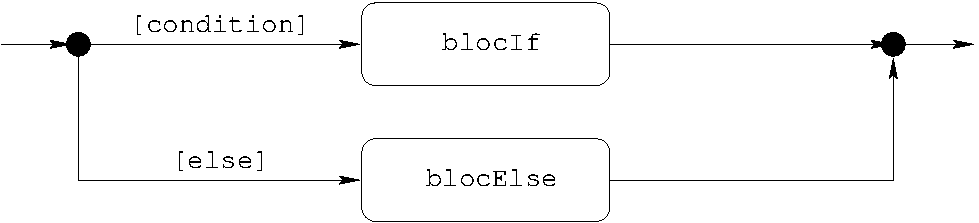
\includegraphics[width=7.5cm]{uml1.pdf}}$$
L'étiquette {\tt [condition]} signifie qu'on passe par la voie correspondante 
si la condition est vérifiée ({\tt True}), sinon on passe par la voie étiquettée
{\tt [else]}.
\end{fig}
}

\begin{ex}[Valeur absolue d'un nombre]\index[algo]{valeur absolue}
L'algorithme qui détermine la valeur absolue $y$ d'un nombre $x$ peut s'écrire de la manière suivante :\\
{\footnotesize\tt
\mbox{}\ \ if x < 0: y = -x\\
\mbox{}\ \ else: y = x
}
\end{ex}
\noindent On commence par tester le signe de $x$ ({\tt if x < 0}), si $x < 0$, alors la valeur absolue $y$
vaut $-x$ ({\tt : y = -x}) sinon ($x \geq 0$) elle vaut $x$ ({\tt else: y = x}).
\exo{td:max}

\begin{ex}[Fonction « porte »]\label{ex:porte}\mbox{}\\
\begin{minipage}{11cm}
On considère la fonction « porte » $f$ dont le graphe est donné ci-contre.
L'alternative suivante permet de calculer $y = f(x)$ :\\
{\footnotesize\tt
\mbox{}\ \ if x < -1 or x > 2: y = 0\\
\mbox{}\ \ else: y = 2
}\exo{td:porte}
\end{minipage}
\hfill
\begin{minipage}{4cm}
\centerline{\includegraphics[width=4cm]{porte.pdf}}
\end{minipage}
\end{ex}
Les exemples \ref{ex:chemin} et \ref{ex:porte} précédents nous montrent
qu'une alternative se comporte comme un aiguillage de chemin de fer 
dans le flux d'instructions (figure \ref{fig:uml1}). 
Un « {\tt if ... else} » ouvre  deux voies correspondant à deux traitements différents, 
et seule une de ces voies sera empruntée (un seul des deux traitements est
exécuté). Mais il y a des situations où deux voies ne suffisent pas : on utilise
alors des alternatives simples en cascade (ou alternatives multiples). 

%-------------------------------------------------------------------------
\subsection{Alternatives multiples}\label{sub:alternatives}
%-------------------------------------------------------------------------
\begin{ex}[Etat de l'eau]
A pression ambiante, l'eau est sous forme de glace si la température
est inférieure à $0^\circ C$, sous forme de liquide si la température
est comprise entre $0^\circ C$ et $100^\circ C$ et sous forme de vapeur
au-delà de $100^\circ C$.
\end{ex}
\marginpar{\footnotesize\em
\begin{fig}[« {\tt if ... else} » imbriqués]\label{fig:uml2}
{\tt 
if condition1 : blocIf1\\
else: \\
\mbox{}\ \ \ \ if condition2 : blocIf2\\
\mbox{}\ \ \ \ else: blocElse}
$${\includegraphics[width=7.5cm]{uml2.pdf}}$$
\end{fig}
\begin{td}[Ouverture d'un guichet]\label{td:guichet}\index[td]{ouverture d'un guichet}
A l'aide d'alternatives simples imbriquées, écrire un algorithme qui détermine 
si un guichet est {\tt 'ouvert'} ou 
{\tt 'fermé'} selon les jours de la semaine ({\tt 'lundi'}, {\tt 'mardi'},
\ldots\ ,{\tt 'dimanche'}) et l'heure de la journée (entre 0h et 24h).
Le guichet est ouvert tous les jours de 8h à 13h et de 14h à 17h 
sauf le samedi après-midi et toute la journée du dimanche.
\end{td}
}
\noindent Un algorithme qui devrait déterminer l'état de l'eau en fonction de
la température doit pouvoir choisir entre trois réponses possibles :
solide, liquide ou vapeur. Une première version de cet algorithme utilise
3 tests simples :\\
{\footnotesize\tt
\mbox{}\ \ if t < 0 : eau = 'glace'\\
\mbox{}\ \ if t >= 0 and t <= 100 : eau = 'liquide'\\
\mbox{}\ \ if t > 100 : eau = 'vapeur'\\
}
Cet algorithme est correct mais va évaluer les 3 conditions 
qui portent sur la même variable
{\tt t} et qui sont exclusives les unes des autres; en effet, si {\tt (t < 0)}, alors
on ne peut pas avoir {\tt (t >= 0 and t <= 100)} ni {\tt (t > 100)}. 
Il est donc inutile d'évaluer les 2 dernières conditions si la première 
est vérifiée, ou d'évaluer la dernière condition si la deuxième est vérifiée.
On préfère donc imbriquer les tests de la manière suivante :\\
{\footnotesize\tt
\mbox{}\ \ if t < 0 : eau = 'glace'\\
\mbox{}\ \ else :\\
\mbox{}\ \ \ \ \ \ if t <= 100 : eau = 'liquide'\\
\mbox{}\ \ \ \ \ \ else: eau = 'vapeur'
}\exo{td:guichet}\\
On commence par évaluer la première condition {\tt (t < 0)}. Si la condition est vérifiée,
on exécute l'affectation {\tt eau = 'glace'}; sinon {\tt (t >= 0)}, on évalue la deuxième 
condition {\tt (t <= 100)} qui en fait est équivalente à {\tt (t >= 0) and (t <= 100)}. 
Si la condition est vérifiée, on exécute l'affectation {\tt eau = 'liquide'};
sinon {\tt (t > 100)}, on exécute l'affectation {\tt eau = 'vapeur'}.
La figure \ref{fig:uml2} illustre le contrôle du flux d'instructions lors de deux
« {\tt if \ldots\ else} » imbriqués : il s'agit de deux aiguillages en cascade.
Afin de simplifier l'écriture des tests imbriqués, on peut contracter le « {\tt else: if} »
en {\tt elif} et obtenir une version plus compacte de l'algorithme, 
strictement équivalente à la version précédente :\\
{\footnotesize\tt
\mbox{}\ \ if t < 0 : eau = 'glace'\\
\mbox{}\ \ elif t <= 100 : eau = 'liquide'\\
\mbox{}\ \ else: eau = 'vapeur'\\
}

\marginpar{\footnotesize\em\vspace*{-1cm}
\begin{fig}[L'alternative multiple]\label{fig:alternatives}
{\tt 
if condition : blocIf\\
elif condition1 : blocElif1\\
elif condition2 : blocElif2\\
\ldots\\
else: blocElse}
$$\includegraphics[width=7.5cm]{uml3.pdf}$$
L'alternative multiple ci-dessus est équivalente
à un ensemble d'alternatives simples imbriquées :\\
{\tt
if condition : blocIf\\
else:\\
\mbox{}\ \ \ \ if condition1 : blocElif1\\
\mbox{}\ \ \ \ else:\\
\mbox{}\ \ \ \ \ \ \ \ if condition2 : blocElif2\\
\mbox{}\ \ \ \ \ \ \ \ else:\\
\mbox{}\ \ \ \ \ \ \ \ \ $\ddots$\\
\mbox{}\ \ \ \ \ \ \ \ \ \ \ \ \ else: blocElse}
\end{fig}
}
\index{if3@{{\tt if\ \ldots\ elif\ \ldots\ else}}}\index{instruction!alternative multiple}
L'instruction « {\tt if} \ldots\ {\tt elif} » teste une première condition (figure \ref{fig:alternatives}). 
Si cette condition est vraie, alors le bloc d'instructions {\tt blocIf} 
est exécuté. Si la première condition est fausse, on teste la deuxième ({\tt condition1}).
Si la deuxième condition est vérifiée, c'est le bloc d'instructions {\tt blocElif1} après le premier « {\tt elif:} » 
(sinon-si) qui est exécuté; sinon on teste la condition suivante ({\tt condition2}).
Si elle est vérifiée, c'est le bloc d'instructions {\tt blocElif2} après le deuxième « {\tt elif:} » 
qui est exécuté et ainsi de suite. Si aucune des conditions n'est vérifiée, c'est le bloc d'instructions
{\tt blocElse} qui est exécuté. Dans tous les cas, un seul des blocs est donc exécuté.

\begin{defin}[alternative multiple]\index[def]{alternative multiple}\index{test!alternative multiple}
L'alternative multiple est une instruction de contrôle du flux d'instructions 
qui permet de choisir entre plusieurs instructions en cascadant des alternatives simples.
\end{defin}


\begin{ex}[Mentions du baccalauréat]
Au baccalauréat, la mention associée à une note sur 20 est
	{\tt 'très bien'} pour les notes supérieures ou égales à 16,
	{\tt 'bien'} pour les notes comprises entre 14 inclus et 16 exclu, 
	{\tt 'assez bien'} pour les notes comprises entre 12 inclus et 14 exclu, 
	{\tt 'passable'} pour les notes comprises entre 10 inclus et 12 exclu et
	{\tt 'insuffisant'} pour les notes strictement inférieures à 10.
\end{ex}
\marginpar{\em\footnotesize
\begin{td}[Catégorie sportive]\label{td:categorie}\index[td]{catégorie sportive}
Ecrire un algorithme qui détermine la catégorie sportive d'un enfant selon
son âge : 
	\begin{itemize}
	\item Poussin de 6 à 7 ans,
	\item Pupille de 8 à 9 ans,
	\item Minime de 10 à 11 ans,
	\item Cadet de 12 ans à 14 ans.
	\end{itemize}
\end{td}}
\noindent On peut utiliser une alternative multiple pour déterminer la mention 
au bac en fonction de la note :\\
{\footnotesize\tt
\mbox{}\ \ if note < 10: mention = 'insuffisant'\\
\mbox{}\ \ elif note < 12: mention = 'passable'\\
\mbox{}\ \ elif note < 14: mention = 'assez bien'\\
\mbox{}\ \ elif note < 16: mention = 'bien'\\
\mbox{}\ \ else: mention = 'très bien'\\
}
\exo{td:categorie}


%-------------------------------------------------------------------------
\section{Boucles}\label{boucles}
%-------------------------------------------------------------------------
\index{itération|see{boucle}}\index{répétition|see{boucle}}
\begin{ex}[Un calcul de pgcd (2)]\label{ex:pgcd2}\index[algo]{algorithme d'{{\sc Euclide}}}
Le plus grand commun diviseur de 2 entiers $a$ et $b$ peut se calculer en appliquant
la relation de récurrence ${\rm pgcd}(a,b) = {\rm pgcd}(b,a\mbox{\tt\%}b)$ jusqu'à ce que le reste
($a\%b$) soit nul.\\
Dans l'exemple \ref{ex:pgcd1} page \pageref{ex:pgcd1}, 
pour calculer le pgcd de $a=12$ et de $b=18$, on appliquait 3 fois de suite
cette relation :
${\rm pgcd}(12,18) = {\rm pgcd}(18,12) = {\rm pgcd}(12,6) = {\rm pgcd}(6,0) = 6$. 
L'algorithme correspondant faisait donc apparaître 3 fois de suite les mêmes instructions 
après l'initialisation des variables $a$ et $b$ :\\
{\tt
\mbox{}\ \ r = a\%b\\
\mbox{}\ \ a = b\\
\mbox{}\ \ b = r}\\
Si nous voulons maintenant calculer le pgcd de $44$ et $5648$, 
il nous faudra répéter 5 fois la même séquence d'instructions pour trouver
que ${\rm pgcd}(44,5648) = 4$. 
\end{ex}
\noindent Ce nouvel exemple de calcul de pgcd soulève au moins 2 questions :
\begin{enumerate}
\item Comment éviter de répéter explicitement plusieurs fois de suite la même 
	séquence d'instructions ? 
\item Comment éviter de savoir à l'avance combien de fois il faut répéter
	la séquence pour obtenir le bon résultat ? 
\end{enumerate}
\marginpar{\footnotesize\em
\begin{fig}[Définition de l'académie (7)]\label{fig:dico7}
{\bf ITÉRATION} n. f. XVe siècle. Emprunté du latin iteratio, « répétition, redite ».
Répétition. MATH. Répétition d'un calcul avec modification de la variable, 
qui permet d'obtenir par approximations successives un résultat satisfaisant.
\end{fig}

\begin{rem}
A propos des instructions itératives,
on parle souvent des boucles « {\tt while} » ou des boucles « {\tt for} » 
dans le jargon des informaticiens.
\end{rem}
}
De nouvelles instructions de contrôle de flux sont introduites pour répondre
à ces questions : les instructions itératives. On parle également de boucles, de répétitions
ou encore d'itérations (figure \ref{fig:dico7}).
Nous distinguerons 2 variantes d'instructions itératives :
$$\begin{tabular}{|l|l|}
\hline
\multicolumn{2}{|c|}{Instructions itératives}\\
\hline
itération conditionnelle & {\begin{minipage}[t]{6cm}\tt while condition : blocWhile \\ \mbox{} \end{minipage}} \\
\hline
parcours de séquence & {\begin{minipage}[t]{7cm}\tt for element in sequence : blocFor \\ \mbox{} \end{minipage}} \\
\hline
\end{tabular}$$
où {\tt while}, {\tt for} et {\tt in} sont des mots réservés, {\tt condition} une expression
booléenne (à valeur {\tt True} ou {\tt False}), {\tt element} un élément de la séquence {\tt sequence}
et {\tt bloc...} un bloc d'instructions.


%-------------------------------------------------------------------------
\subsection{Itération conditionnelle}
%-------------------------------------------------------------------------
\marginpar{\footnotesize\em
\begin{fig}[Boucle {\tt while}]\label{fig:while}
{\tt while condition : blocWhile}
$$\includegraphics[width=7.5cm]{uml4.pdf}$$
\end{fig}}
L'instruction « {\tt while} » \index{while@{{\tt while}}} permet de répéter plusieurs fois une même instruction 
(figure \ref{fig:while}) : le bloc d'instructions {\tt blocWhile} est exécuté tant que
({\em while}) la condition est vérifiée. On arrête dès que la condition est fausse; 
on dit alors qu'on « sort » de la boucle. 

On commence par tester la condition; si elle
est vérifiée, on exécute le bloc d'instructions {\tt blocWhile} 
(encore appelé le «~corps~» de la boucle) puis on reteste la condition : 
la condition est ainsi évaluée avant chaque exécution du corps 
de la boucle; si la condition est à nouveau vérifiée on réexécute le bloc 
d'instructions {\tt blocWhile} (on dit qu'on « repasse » dans la boucle)
et ainsi de suite jusqu'à ce que la condition devienne fausse, 
auquel cas on « sort » de la boucle.

\begin{defin}[itération conditionnelle]\index[def]{itération conditionnelle}\index{boucle!itération conditionnelle}
L'itération conditionnelle est une instruction de contrôle du flux d'instructions
qui permet sous condition préalable de répéter zéro ou plusieurs fois la même instruction.
\end{defin}

\begin{ex}[Table de multiplication]\label{ex:table}\index[algo]{tables de multiplication}
On cherche à écrire un algorithme qui affiche la table de multiplication
d'un nombre $n$ quelconque.\\
Exemple : $n = 9 \rightarrow\ $
\begin{py}{3cm}
\begin{verbatim}
1 * 9 = 9
2 * 9 = 18
3 * 9 = 27
4 * 9 = 36
5 * 9 = 45
6 * 9 = 54
7 * 9 = 63
8 * 9 = 72
9 * 9 = 81
\end{verbatim}
\end{py}
\hfill
\begin{minipage}[t]{8cm}
L'affichage ci-contre est obtenu par l'algorithme suivant :
\begin{py}{5cm}
\begin{verbatim}
n = 9
i = 1
while i < 10:
    print(i, '*', n, '=', i*n)
    i = i + 1
\end{verbatim}
\end{py}
\end{minipage}
\end{ex}

\noindent L'algorithme précédent commence par initialiser {\tt n} et le multiplicateur {\tt i}.
Ensuite, puisque {\tt i < 10}, on rentre dans la boucle; la première instruction
{\tt print} affiche successivement la valeur de {\tt i}, une {\tt *}, 
la valeur de {\tt n}, le signe {\tt =} puis la valeur du produit {\tt i*n}, 
soit au premier passage : {\tt 1 * 9 = 9}. L'instruction suivante incrémente {\tt i} qui devient
ainsi égal à {\tt 2} ({\tt 1 + 1}). Les deux instructions du corps de la boucle {\tt while} ayant 
été exécutées, on reteste la condition {\tt i < 10}; elle est à nouveau vérifiée puisque {\tt i}
vaut maintenant {\tt 2}. On repasse alors dans la boucle où on affiche {\tt 2 * 9 = 18} et où on
incrémente {\tt i} qui vaut maintenant {\tt 3} ({\tt 2 + 1}). On réitère ces opérations jusqu'à 
ce que {\tt i} soit égal à {\tt 10} ({\tt 9 + 1}); entre-temps les 7 autres lignes de la table de 
multiplication par {\tt 9} ont été affichées. Lorsque {\tt i} vaut {\tt 10}, la condition {\tt i < 10}
n'est plus vérifiée et on « sort » de la boucle {\tt while}.
\exo{td:etoile}

\marginpar{\footnotesize\em
\begin{td}[Dessin d'étoiles (1)]\label{td:etoile}\index[td]{dessin d'étoiles}
Ecrire un algorithme itératif qui affiche les $n$ lignes suivantes (l'exemple
est donné ici pour $n=6$) : \\
\begin{minipage}[t]{2cm}\tt
******\\
*****\\
****\\
***\\
**\\
*
\end{minipage}
\hfill
\begin{minipage}[t]{3cm}
Rappel \python\ : \\
{\tt
\mbox{}\ \ \ \ >>> 5*'r'\\
\mbox{}\ \ \ \ 'rrrrr'\\
\mbox{}\ \ \ \ >>> 2*'to'\\
\mbox{}\ \ \ \ 'toto'
}
\end{minipage}
\end{td}}
Dans une itération conditionnelle, la condition doit évoluer au cours des différents passages
dans la boucle afin de pouvoir sortir de la boucle. C'est le cas de la boucle {\tt while}
de l'exemple \ref{ex:table} ci-dessus; à chaque passage dans la boucle, le
multiplicateur {\tt i} est incrémenté : ainsi, partant de la valeur initiale {\tt i = 1},
{\tt i} deviendra nécessairement égal à {\tt 10} après 9 passages dans la boucle.

En ce qui concerne le nombre de passages dans la boucle, deux cas extrèmes peuvent se produire : 
\begin{itemize}
\item la condition n'est pas vérifiée la première fois : 
	on ne passe alors jamais dans la boucle.
	
	Exemple : 
	\begin{py}{5cm}
	\begin{verbatim}
	x = 4
	y = 0
	while x < 0 : y = y + x
	\end{verbatim}
	\end{py}\hfill
	\begin{minipage}[t]{7.5cm}\footnotesize
	$x$ est positif; la condition $x < 0$ n'est donc pas vérifiée la première
	fois : on ne rentre pas dans la boucle.
	\end{minipage}
\item la condition n'est jamais fausse : on ne sort jamais de la boucle; 
	on dit qu'on a affaire à une boucle « sans fin ».

	Exemple : 
	\begin{py}{5cm}
	\begin{verbatim}
	x = 4
	y = 0
	while y >= 0 : y = y + x
	\end{verbatim}
	\end{py}\hfill
	\begin{minipage}[t]{7.5cm}\footnotesize
	$y$ est initialement nul : on rentre dans la boucle;
	l'instruction du corps de la boucle ne peut qu'incrémenter $y$
	puisque $x$ est positif : $y$ sera donc toujours positif et on 
	ne sortira jamais de la boucle.
	\end{minipage}
\end{itemize}
Le cas de la boucle « sans fin » est évidemment dû le plus souvent à une erreur involontaire
qu'il faut savoir détecter assez vite pour éviter un programme qui « tourne » indéfiniment
sans s'arrêter.

\marginpar{\footnotesize\em
\begin{rem}Une erreur classique de l'apprenti informaticien est de ne pas faire évoluer
la condition d'une boucle {\tt while} : il « tombe » alors dans une boucle « sans fin »
comme dans l'exemple ci-dessous :\\
\begin{minipage}[t]{2.75cm}\tt
\mbox{}\ \ k = 1\\
\mbox{}\ \ p = x\\
\mbox{}\ \ while k <= n:\\
    \mbox{}\ \ \ \ p = p*x
\end{minipage}
\hfill
\begin{minipage}[t]{5cm}
On entre dans la boucle; on calcule la nouvelle valeur de {\tt p}
puis on reteste la condition {\tt k <= n}. Mais entre-temps {\tt k}
n'a pas évolué (il n'a pas été incrémenté) et donc la condition
reste vraie et restera toujours vraie : l'exécution ne sortira plus de la boucle.
\end{minipage}
\end{rem}
}
\begin{ex}[Fonction puissance]\label{ex:puissance}\index[algo]{fonction puissance}
La puissance entière $p$ d'un nombre $x$ est définie par :
$\displaystyle p = x^n = \prod_{k=1}^{n} x = \underbrace{x\cdot x\cdot x\cdots x}_{n\ \rm fois}$ .
\end{ex}
\noindent Pour calculer $p$ « de tête », nous calculons successivement $x$, $x^2$, $x^3$\ldots,
$x^{n-1}$ et $x^n$ en mémorisant à chaque étape la puissance courante $x^k$ et en multipliant
simplement cette puissance par $x$ pour obtenir la puissance immédiatement supérieure $x^{k+1}$.
On s'arrête quand $k = n$ : on a alors le résultat attendu ($p = x^n$).
Cet algorithme peut s'écrire directement :\\
\mbox{}\ \ \begin{py}{3cm}
\begin{verbatim}
k = 1
p = x
while k < n:
    p = p*x
    k = k + 1
\end{verbatim}
\end{py}
\hfill
\begin{minipage}[t]{12cm}\footnotesize
On commence par initialisé l'exposant $k$ à 1 et la puissance $p$ recherchée 
avec la valeur de $x^k = x^1 = x$ ({\tt p = x}). 
Ensuite, pour chaque valeur de $k < n$,
on multiplie la puissance courante $p$ par $x$ ({\tt p*x}) qui devient la nouvelle
puissance courante ({\tt p = p*x}) et on n'oublie pas d'incrémenter l'exposant $k$; ainsi
à la fin de chaque itération, on a toujours $p = x^k\ \forall k \in [1;n]$.
\end{minipage}\\
\exo{td:factorielle}

\marginpar{\footnotesize\em
\begin{td}[Fonction factorielle]\label{td:factorielle}\index[algo]{fonction factorielle}\index[td]{fonction factorielle}
Ecrire un algorithme qui calcule $n! = 1\cdot 2\cdot 3\cdot \ldots \cdot (n-1)\cdot n$.
\end{td}
}
Dans les exemples \ref{ex:table} et \ref{ex:puissance} précédents, on savait à l'avance
combien de fois on devait passer dans les boucles : 9 fois pour afficher une table de 
multiplication et $n$ fois pour calculer $x^n$. Mais ce n'est pas toujours le cas comme 
nous allons le constater dans les deux exemples suivants qui permettent de calculer 
respectivement la fonction exponentielle (exemple \ref{ex:exp} : $e^x$) 
et le pgcd de 2 nombres (exemple \ref{ex:pgcd3} : ${\rm pgcd}(a,b)$).

\begin{ex}[Fonction exponentielle]\label{ex:exp}\index[algo]{développements limités}
La fonction exponentielle peut être calculée en fonction de son d\'eveloppement 
en série entière. 
$$\displaystyle y = \exp(x) \approx \sum_{k=0}^{n} u_k = \sum_{k=0}^{n} \frac{x^{k}}{k!} = 
	1 + x + \frac{x^2}{2} + \ldots + \frac{x^{n}}{n!}$$
Les calculs seront arr\^et\'es lorsque la valeur absolue du terme $u_k$ sera inf\'erieure 
\`a un certain seuil $s$ ($0 < s < 1$). On n'utilisera ni la fonction {\em puissance} ($x^n$) 
ni la fonction {\em facto\-riel\-le} ($n!$) pour effectuer le calcul de $\exp(x)$.
\end{ex}
\noindent Pour ce calcul, on pourrait avoir la même démarche que dans l'exemple \ref{ex:puissance}
de la puissance entière; à savoir, on calcule le premier terme
de la série ($x^0/0! = 1$), on le mémorise dans $y$, on calcule le $2^{\grave eme}$ terme ($x^1/1! = x$) 
et on l'ajoute à la valeur de $y$ précédemment mémorisée ($1 + x$), on calcule le $3^{\grave eme}$ 
terme ($x^2/2! = x^2/2$), on l'ajoute à $y$ ($1 + x + x^2/2$) et ainsi de suite jusqu'à ce que 
le nouveau terme calculé vérifie la 
condition d'arrêt imposée ($|u_k| < s$). Mais chaque évaluation d'un nouveau terme fait intervenir 
{\em a priori} les fonctions puissance ($x^k$) et factorielle ($n!$)\ldots qui sont très coûteuses 
en temps de calcul. On préfère remarquer que le terme $u_{k+1}$ peut s'exprimer simplement en 
fonction du terme précédent $u_k$ selon la relation de récurrence :
$$u_{k+1} = \frac{x^{k+1}}{(k+1)!} = \frac{x}{k+1}\cdot\frac{x^{k}}{k!} = \frac{x}{k+1}u_k$$
et qu'il est donc possible de mémoriser à chaque étape $u_k$ pour calculer le terme suivant 
$u_{k+1}$ sans utiliser ni la fonction puissance, ni la fonction factorielle. 
On obtient alors l'algorithme suivant :\\
\mbox{}\ \ \begin{py}{3cm}
\begin{verbatim}
k = 0
u = 1
y = u
while fabs(u) > s:
    u = u*x/(k+1)
    y = y + u
    k = k + 1
\end{verbatim}
\end{py}
\marginpar{\em\footnotesize
\begin{td}[Fonction sinus]\label{td:sinus}\index[algo]{développements limités}\index[td]{fonction sinus}
Ecrire un algorithme qui calcule de manière itérative la fonction sinus
en fonction de son d\'eveloppement en série entière.\\
$\displaystyle\sin(x) \approx \sum_{k=0}^{n} u_k = \sum_{k=0}^{n} (-1)^k\frac{x^{2k+1}}{(2k+1)!}\\
\mbox{}\hfill = x - \frac{x^3}{6} + \frac{x^5}{120} + \ldots + (-1)^n\frac{x^{2n+1}}{(2n+1)!}$\\
Les calculs seront arr\^et\'es lorsque la valeur absolue du terme $u_k$ sera 
inf\'erieure \`a un certain seuil $s$ ($0 < s < 1$). On n'utilisera ni la fonction 
{\em puissance} ($x^n$) ni la fonction {\em facto\-riel\-le} ($n!$) pour effectuer
le calcul de $\sin(x)$.
\end{td}}
\hfill
\begin{minipage}[t]{12cm}\footnotesize
On initialise l'indice {\tt k} à {\tt 0}, le terme {\tt u} (= $u_k$) à la valeur du premier
terme de la série ($x^0/0! = 1$) et {\tt y} à ce premier terme ({\tt y = u}). Puis, tant que la valeur absolue
de $u_k$ ({\tt fabs(u)}) est supérieure au seuil {\tt s}, on calcule le terme suivant $u_{k+1}$ en
utilisant la relation de récurrence obtenue ci-dessus ({\tt u = u*x/(k+1)}) : le nouveau terme $u_{k+1}$
est égal à l'ancien terme $u_k$ multiplié par $x/(k+1)$; on ajoute $u_{k+1}$ à la somme courante $y$
({\tt y = y + u}) et on recommence sans oublier d'incrémenter {\tt k} ({\tt k = k + 1}). 
A la fin de chaque itération, on a toujours $\displaystyle y = \sum_{i=0}^{k} u_i$.
\end{minipage}\\
Ici, on connait la condition d'arrêt de la boucle ($|u_k| < s$) mais on ne sait pas {\em a priori} 
combien de fois on passera dans la boucle : on ne connait pas l'ordre $n$ pour lequel on arrêtera le
développement de la série entière.
\exo{td:sinus}


\begin{ex}[Un calcul de pgcd (3)]\label{ex:pgcd3}
\index[algo]{algorithme d'{{\sc Euclide}}}\mbox{}
On considère à nouveau la relation de récurrence qui caractérise
le pgcd de 2 entiers $a$ et $b$ (voir exemples \ref{ex:pgcd1} et \ref{ex:pgcd2}) : 
${\rm pgcd}(a,b) = {\rm pgcd}(b,a\mbox{\tt\%}b)$. Cette relation nous dit de remplacer
$a$ par $b$ et $b$ par $r = a\%b$ autant de fois que possible jusqu'à ce que le reste
soit nul (${\rm pgcd}(a,0) = a$). Ce qui conduit à l'algorithme suivant :\\
\mbox{}\ \ \begin{py}{2cm}
\begin{verbatim}
while b != 0:
    r = a%b
    a = b
    b = r
\end{verbatim}
\end{py}
\hfill
\begin{minipage}[t]{12cm}\footnotesize
A la fin de chaque passage dans le corps de la boucle, $a$, $b$ et $r$ prennent
successivement les valeurs suivantes ($r$ n'est pas connu avant la boucle) :
$$\begin{tabular}{|l|c|c|c|}
\cline{2-4}
\multicolumn{1}{l|}{}                 &$a$ & $b$ & $r$\\
\hline
avant la boucle  & 12 & 18 & ?\\
\hline
$1^{er}$ passage & 18 & 12 & 12 \\
$2^{\grave eme}$ passage & 12 & 6 & 6\\
$3^{\grave eme}$ passage & 6 & 0 & 0\\
\hline
après la boucle  & 6  & 0 & 0\\
\hline
\end{tabular}$$
\end{minipage}
\end{ex}

\noindent Cet algorithme de calcul de pgcd est connu sous le nom 
d'algorithme d'Euclide (figure \ref{fig:euclide}) et fait partie des grands classiques 
de l'algorithmique.
\exo{td:euclide}\\
Là encore, la condition d'arrêt est connue ($b \neq 0$) mais pas le nombre de passages dans la boucle.
\exo{td:division}
\marginpar{\footnotesize\em
\begin{fig}[Euclide]\label{fig:euclide}
Euclide (né vers -325, mort vers -265) était un mathématicien de la Grèce antique, auteur des «~Éléments~», 
qui sont considérés comme l'un des textes fondateurs des mathématiques modernes.
En particulier, le livre 7 traite de l'arithmétique : il y définit la division 
que l'on appelle division euclidienne et un algorithme pour calculer le plus grand commun diviseur 
de deux nombres, connu sous le nom d'algorithme d'Euclide.
\end{fig}

\begin{td}[Algorithme d'Euclide]\label{td:euclide}\index[td]{algorithme d'{{\sc Euclide}}}
Dans la tradition grecque, en comprenant un nombre entier comme une longueur, 
un couple d'entiers comme un rectangle, leur pgcd est la taille du plus grand 
carré permettant de carreler ce rectangle. L'algorithme décompose ce rectangle 
en carrés, de plus en plus petits, par divisions euclidiennes successives, 
de la longueur par la largeur, puis de la largeur par le reste, 
jusqu'à un reste nul.\\
Faire la construction géométrique «~à la grecque antique~» qui permet de déterminer 
le pgcd $d$ de $a=21$ et $b=15$ ($d=3$).
\end{td}

\begin{td}[Division entière]\label{td:division}\index[td]{division entière}
Ecrire un algorithme itératif qui calcule le quotient $q$ et le reste $r$ de la 
division entière $a\div b$ ($a = bq+r$).\\
On n'utilisera pas les opérateurs prédéfinis {\tt /} et {\tt \%} mais
on pourra s'inspirer du TD \ref{td:seq1} page \pageref{td:seq1}.
\end{td}}

Dans tous les cas, que l'on connaisse ou non {\em a priori} le nombre de passages dans la boucle, on peut
toujours utiliser l'itération conditionnelle (boucle {\tt while}) pour répéter plusieurs fois un bloc
d'instructions à condition de connaître la condition d'arrêt pour sortir de la boucle.
\begin{itemize}
\item Lorsqu'on connaît {\em a priori} le nombre de passages dans la boucle (voir exemples
	\ref{ex:table} et \ref{ex:puissance}), il suffit de définir un compteur qui compte le nombre
	de fois où on passe dans la boucle : le multiplicateur {\tt i} dans l'exemple de la table
	de multiplication et l'exposant {\tt k} dans le calcul de la puissance.
	On initialise correctement ce compteur avant la boucle ({\tt i = 1} ou {\tt k = 1} selon
	l'exemple considéré), on incrémente le compteur dans la boucle ({\tt i = i + 1} ou {\tt k = k + 1})
	et on sort de la boucle lorsque ce compteur dépasse le nombre de fois connu
	où on doit passer dans la boucle ({\tt i < 10} ou {\tt k <= n}).
\item Lorsqu'on ne connaît pas {\em a priori} le nombre de passages dans la boucle (voir exemples
	\ref{ex:exp} et \ref{ex:pgcd3}), il faut absolument déterminer la condition d'arrêt
	de l'algorithme : $|u_k| < s$ pour le calcul de $e^x$ et $b = 0$ dans l'exemple du pgcd.
	Il faut également s'assurer que cette condition sera bien atteinte au bout d'un certain 
	nombre de passages dans la boucle : dans le calcul du pgcd par exemple, le reste $r$ de la division 
	$a \div b$ ne peut être qu'inférieur au diviseur $b$ et comme $b$ est remplacé par $r$ dans le corps
	de la boucle, $b$ ne peut que diminuer et atteindre $0$ au bout du compte.
\end{itemize}


%-------------------------------------------------------------------------
\subsection{Parcours de séquences}\label{sub:parcours}
%-------------------------------------------------------------------------
Il est fréquent de manipuler des suites ordonnées d'éléments comme 
les chaînes de caractères (exemple : {\tt s = "123"}), les tableaux
(exemple : {\tt t = [1,2,3]}) et les n-uplets (exemple : {\tt u = 1,2,3}).
Chaque élément d'une séquence est accessible par son rang dans la séquence 
grâce à l'opérateur « crochets » : {\tt sequence[rang]} (exemples : {\tt s[1]}, {\tt t[2]} ou {\tt u[0]}) et par convention, 
le premier élément d'une séquence a le rang {\tt 0} (exemples : {\tt s[1]} est le $2^{\grave eme}$
élément de la chaîne {\tt s}, {\tt t[2]} le $3^{\grave eme}$ élément du tableau {\tt t}
et {\tt u[0]} le $1^{er}$ élément du n-uplet {\tt u}).

\begin{py}{4cm}
\begin{verbatim}
>>> s = "123"
>>> s[1]
'2'
\end{verbatim}
\end{py}
\hfill
\begin{py}{4cm}
\begin{verbatim}
>>> t = [1,2,3]
>>> t[2]
3
\end{verbatim}
\end{py}
\hfill
\begin{py}{4cm}
\begin{verbatim}
>>> u = 1,2,3
>>> u[0]
1
\end{verbatim}
\end{py}

\begin{defin}[séquence]\index[def]{séquence}
Une séquence est une suite ordonnée d'éléments, éventuellement vide, 
accessibles par leur rang dans la séquence.
\end{defin}

\marginpar{\footnotesize\em
\begin{rem}
Les éléments d'une chaîne de caractères sont eux-mêmes des chaînes de caractères
à 1 seul caractère.

\begin{py}{4cm}\tt
\mbox{}\ \ >>> s = 'a4b2'\\
\mbox{}\ \ >>> s[1]\\
\mbox{}\ \ '4'\\
\mbox{}\ \ >>> s[3]\\
\mbox{}\ \ '2'
\end{py}
\end{rem}}

\noindent Les principales opérations sur les séquences sont listées 
dans le tableau ci-dessous (d'après \cite{gruet})\label{cite:gruet2}.\index{langage!{{\sc Python}}!séquences}
$$\begin{tabular}{|l|p{9cm}|}
\hline 
\makebox[5.5cm][l]{\bf Operation} &	\bf Result 	\\
\hline
\tt x in s      & {\tt True} if an item of {\tt s} is equal to {\tt x}, else {\tt False} \\ 	
\tt x not in s 	& {\tt False} if an item of {\tt s} is equal to {\tt x}, else {\tt True}\\
\hline 	
\tt s1 + s2 	& the concatenation of {\tt s1} and {\tt s2}\\ 	 
\tt s * n, n*s 	& {\tt n} copies of {\tt s} concatenated \\	
\hline
\tt s[i] 	& {\tt i}'th item of {\tt s}, origin {\tt 0}\\ 	
\tt s[i: j]     & \\
\tt s[i: j:step]& Slice of {\tt s} from {\tt i} (included) to {\tt j}(excluded). 
                  Optional {\tt step} value, possibly negative (default: {\tt 1}). \\	
\hline
\tt len(s) 	& Length of s \\	 
\tt min(s) 	& Smallest item of s \\	
\tt max(s) 	& Largest item of s \\
\hline
\hline
\tt range([start,] end [, step]) & Returns list of ints from {\tt >=} {\tt start} and {\tt <} {\tt end}.\newline
	With 1 arg, list from {\tt 0..arg-1}\newline
	With 2 args, list from {\tt start..end-1}\newline
	With 3 args, list from {\tt start} up to {\tt end} by {\tt step}\\
\hline
\end{tabular}$$
La dernière fonction de ce tableau crée un tableau d'entiers compris entre {\tt start} inclus
(= 0 par défaut) et {\tt end} exclus par pas de {\tt step} (= 1 par défaut).

\begin{py}{5cm}
\begin{verbatim}
>>> range(3)
[0, 1, 2]
>>> range(3,9,2)
[3, 5, 7]
>>> range(7,0,-1)
[7, 6, 5, 4, 3, 2, 1]
\end{verbatim}
\end{py}
\hfill
\begin{py}{5cm}
\begin{verbatim}
>>> s = "bonjour"
>>> range(len(s))
[0, 1, 2, 3, 4, 5, 6]
>>> t = [4,2,6,5,3]
>>> range(max(t),min(t),-1)
[6, 5, 4, 3]
\end{verbatim}
\end{py}
\hfill
\begin{py}{5cm}
\begin{verbatim}
>>> u1 = 10,12,14
>>> u2 = 'a','b','c'
>>> range(len(u1+u2))
[0, 1, 2, 3, 4, 5]
>>> range(len(2*u2[0:2]))
[0, 1, 2, 3]
\end{verbatim}
\end{py}
\vspace*{1mm}

\begin{ex}[Affichage caractère par caractère]\label{ex:caractere}
L'algorithme suivant affiche les caractères d'une chaîne {\tt s}, un par ligne :

\begin{py}{5cm}\tt
i = 0\\
while i < len(s):\\
\mbox{}\ \ \ \ print(s[i])\\
\mbox{}\ \ \ \ i = i + 1
\end{py} 
\hfill
\begin{py}{10cm}
On se place au début de la chaîne (rang {\tt i = 0}) et, tant qu'on est à l'intérieur de la chaîne
({\tt i < len(s)}), on affiche l'élément courant {\tt s[i]}. Le rang {\tt i} prend successivement
les valeurs {\tt 0}, {\tt 1}, {\tt 2} \ldots\ {\tt len(s)-1} ({\tt len(s)} exclus).
\end{py}\\
\exo{td:caractere}
\end{ex}
\marginpar{\footnotesize\em\vspace*{-2cm}
\begin{td}[Affichage inverse]\label{td:caractere}\index[td]{affichage inverse}
Ecrire un algorithme qui affiche les caractères d'une chaîne {\tt s},
un par ligne en partant de la fin de la chaîne.
\end{td}

\begin{td}[Parcours inverse]\label{td:parcours}\index[td]{parcours inverse}
Ecrire un algorithme qui parcourt en sens inverse une séquence {\tt s}
quelconque (du dernier élément au premier élément).
\end{td}
\begin{fig}[Boucle {\tt for}]\label{fig:for}
\tt for element in s : blocFor\\
\centerline{\includegraphics[width=7.5cm]{uml7.pdf}}
\end{fig}

\begin{td}[Suite arithmétique (2)]\label{td:suiteArit2}\index[algo]{suites numériques}
\begin{enumerate}
\item Ecrire un algorithme qui calcule de manière itérative la somme $s = \sum_0^n u_k$ des $n$ premiers 
	termes d'une suite arithmétique $u_k = a + r\cdot k$. On utilisera une boucle {\tt for}.
\item Comparer l'efficacité de cette approche itérative avec le calcul du TD \ref{td:suiteArit} 
	page \pageref{td:suiteArit}.
\end{enumerate}
\end{td}}

\noindent L'affichage précédent nous a conduits à parcourir la chaîne {\tt s}
du premier élément ({\tt i = 0}) au dernier élément ({\tt i = len(s)-1}).
On peut généraliser cet exemple au parcours d'une séquence {\tt s} quelconque, 
du premier élément au dernier élément (parcours direct) :

\index{boucle!parcours de séquence}
\begin{py}{5cm}
\begin{verbatim}
i = 0
while i < len(s):
    # traiter s[i]
    i = i + 1
\end{verbatim}
\end{py}
\hfill
\begin{py}{10cm}
Se placer au début de la séquence : initialiser un entier {\tt i} qui représentera
le rang dans la séquence (rang initial : {\tt i = 0}); puis tant qu'on est dans
la séquence (condition : {\tt 0 <= i < len(s)}), traiter l'élément courant {\tt s[i]} 
et passer à l'élément suivant ({\tt i = i + 1}).
\end{py}\\
\exo{td:parcours}
 
\noindent Il existe une instruction de contrôle adaptée au parcours de séquence (figure \ref{fig:for}) :
\index{for@{{\tt for}}}
$$\fbox{\tt for element in sequence : blocFor}$$
$$\begin{minipage}{6.5cm}équivalente à : 
\begin{py}{4cm}
\begin{verbatim}
i = 0
while i < len(s):
    element = sequence[i]
    blocFor
    i = i + 1
\end{verbatim}
\end{py}
\end{minipage}$$
\noindent Ainsi, l'algorithme de l'exemple \ref{ex:caractere} ci-dessus peur se réécrire 
simplement sous la forme :\\
{\tt \mbox{}\ \ for element in s : print(element)}\\
De même, l'algorithme de calcul de la fonction puissance (exemple \ref{ex:puissance})
peut s'écrire avec une boucle {\tt for} :\\
{\tt
\mbox{}\ \ p = x\\
\mbox{}\ \ for i in range(n) : p = p*x}
\exo{td:suiteArit2}


%-------------------------------------------------------------------------
\subsection{Imbrications de boucles}
%-------------------------------------------------------------------------
De la même manière que l'on peut cascader des alternatives simples
(voir section \ref{sub:alternatives}), on peut encapsuler une boucle 
dans une autre boucle.\index{boucle!boucles imbriquées}

\begin{ex}[Tables de multiplication]\label{ex:tables}\index[algo]{tables de multiplication}
Nous avons affiché une table de multiplication dans l'exemple \ref{ex:table}
page \pageref{ex:table}. Nous voulons maintenant afficher les 9 premières tables de 
multiplication en réutilisant l'algorithme d'affichage d'une seule table. Il nous suffit
pour cela de répéter 9 fois l'algorithme d'affichage d'une table en incrémentant 
le multiplicande $n$ à chaque itération :\\
\mbox{}\ \ \begin{py}{5cm}
\begin{verbatim}
n = 1
while n <= 9:
    i = 1
    while i < 10:
        print(i, '*', n, '=', i*n)
        i = i + 1
    n = n + 1
\end{verbatim}
\end{py}
\hfill
\begin{minipage}[t]{9.5cm}\footnotesize
On initialise {\tt n} à {\tt 1} (on commence par la table de multiplication de $1$),
puis on entre dans la boucle qui fera varier {\tt n} de {\tt 1} à {\tt 9} ({\tt while n <= 9}).
On exécute l'algorithme d'affichage d'une table (exemple \ref{ex:table}) et à la sortie de
cet algorithme, on n'oublie pas d'incrémenter {\tt n} ({\tt n = n + 1}) pour passer à la
table suivante. Et ainsi de suite jusqu'à la table de $9$. Quand $n = 9$, son incrémentation
lui affecte la valeur {\tt 10}, ce qui rend fausse la condition de la boucle ({\tt n <= 9}) :
on sort alors de la boucle extérieure. 
\end{minipage}
\end{ex}
\exo{td:etoile2}

\marginpar{\footnotesize\em\vspace*{-4cm}
\begin{td}[Dessin d'étoiles (2)]\label{td:etoile2}\index[td]{dessin d'étoiles}
Reprendre le TD \ref{td:etoile} page \pageref{td:etoile} en supposant qu'on ne peut 
afficher qu'une étoile à la fois (on s'interdit ici la possibilité d'écrire
{\tt 5*'*'} à la place de {\tt '*****'} par exemple).
\end{td}
\begin{rem}Dans le langage {\sc Pascal}, les blocs d'instructions sont délimités par les 
mots-clés explicites {\tt begin \ldots\ end}. En langage {\sc C}, les blocs d'instructions 
sont délimités par des accolades ({\tt \{ \ldots\ \}}). En {\sc Python}, les blocs sont 
caractérisés par l'indentation identique de chaque instruction du bloc.
\end{rem}

\begin{fig}[Blocs d'instructions]\label{fig:bloc}\mbox{}\\
\centerline{\includegraphics[height=5cm]{bloc.pdf}}
\end{fig}}
\noindent Cet exemple d'instruction composée pose explicitement le problème de la définition
d'un bloc d'instructions : où commence et où termine un bloc d'instructions ?
\index{instruction!bloc d'instructions} 
En effet, l'instruction {\tt n = n + 1} fait-elle partie du bloc de la boucle intérieure
({\tt while i < 10:}) ou du bloc de la boucle extérieure ({\tt while n <= 9:}) ?

Les instructions composées ont toujours la même structure : 
une ligne d'en-tête terminée par un double point ({:}), suivie
d'une ou de plusieurs instructions indentées (décalées à droite)
sous cette ligne d'en-tête (figure \ref{fig:bloc}).

\index{langage!{{\sc Python}}!bloc d'instructions} 
\begin{py}{5cm}
\begin{verbatim}
ligne d'en-tête:
    première instruction du bloc
    ...
    dernière instruction du bloc
    \end{verbatim}
\end{py}

\noindent S'il y a plusieurs instructions indentées sous la ligne d'en-tête, elles doivent l'être exactement au
même niveau (décalage de 4 caractères espace, par exemple). Ces instructions indentées
constituent ce qu'on appellera désormais un bloc d'instructions. Un bloc d'instructions est une
suite d'instructions formant un ensemble logique, qui n'est exécuté que dans certaines conditions
définies dans la ligne d'en-tête. Dans l'exemple précédent, les deux lignes
d'instructions indentées sous la ligne contenant l'instruction « {\tt while i < 10:} » constituent un même 
bloc logique : ces deux lignes ne sont exécutées -- toutes les deux -- que si la condition testée 
avec l'instruction {\tt while} est vérifiée, c'est-à-dire si le multiplicateur {\tt i}
est tel que {\tt 1 <= i < 10}.

\begin{ex}[Tables de vérité]\label{ex:verite}\index[algo]{tables de vérité}
Pour afficher les tables de vérité des opérateurs logiques
de base (voir section \ref{sub:cond}) :
négation (non, {\em not}, $\overline{a}$), 
disjonction (ou, {\em or}, $a+b$) et 
conjonction (et, {\em and}, $a\cdot b$),
on peut utiliser 2 boucles {\tt for} imbriquées :
	
	Exemple : $a\cdot b$ 
	
	\begin{minipage}[t]{5cm}
	$\begin{array}[t]{|c|c|c|}
	\hline
	a & b & a\cdot b\\
	\hline
	0 & 0 & 0\\
	0 & 1 & 0\\
	1 & 0 & 0\\
	1 & 1 & 1\\
	\hline
	\end{array}$
	\end{minipage}
	\hspace*{1cm}
	\begin{py}{5cm}
	\begin{verbatim}
	>>> for a in  [0,1]:
	...   for b in [0,1]:
	...     print(a, b, a and b)
	... 
	0 0 0
	0 1 0
	1 0 0
	1 1 1
	\end{verbatim}
	\end{py}
	\exo{td:booleens2}
\end{ex}


\marginpar{\footnotesize\em\vspace*{-2cm}
\begin{td}[Opérateurs booléens dérivés (2)]\label{td:booleens2}\index[td]{opérateurs booléens dérivés}
A l'aide d'itérations imbriquées, afficher les tables de vérité des 
opérateurs logiques dérivés (voir TD \ref{td:booleens1}) : 
ou exclusif ({\em xor}, $a \oplus b$), 
non ou ({\em nor}, $\overline{a+b}$), 
non et ({\em nand}, $\overline{a\cdot b}$), 
implication ($a \Rightarrow b$) et  
équivalence ($a \Leftrightarrow b$).
\end{td}

\begin{fig}[Nid d'abeilles]\label{fig:abeilles}\mbox{}\\
\centerline{\includegraphics[width=7.5cm]{motif.pdf}}
\end{fig}}
\begin{ex}[Nid d'abeilles]\label{ex:abeille}\index[algo]{nid d'abeilles}\index[td]{nid d'abeilles}
Un motif en nid d'abeilles est
formé de $n\times m$ hexagones en quinconce comme sur la figure \ref{fig:abeilles}
ci-contre.\\
\end{ex}

\noindent Pour dessiner un tel motif, il faut d'abord savoir dessiner un hexagone de côté {\tt a} 
en utilisant les instructions {\em à la {\sc Logo}} de l'annexe \ref{logo} page \pageref{logo} :

\begin{py}{3cm}
\begin{verbatim}
for k in range(6):
    forward(a)
    left(60)
\end{verbatim}
\end{py}
\vspace*{1mm}

\noindent puis une colonne de {\tt m} hexagones de côté {\tt a} à l'abscisse {\tt x0} :

\begin{py}{3cm}
\begin{verbatim}
for j in range(m):
    y0 = a*sqrt(3)*(1/2. - j)
    up()
    goto(-x0,-y0)
    down()
    for k in range(6):
        forward(a)
        left(60)
\end{verbatim}
\end{py}
\vspace*{1mm}

\noindent et enfin {\tt n} colonnes de {\tt m} hexagones en quinconce :

\begin{py}{3cm}
\begin{verbatim}
for i in range(n):
    x0 = -3*i*a/2.
    for j in range(m):
        y0 = a*sqrt(3)*(1/2.*(i%2) - j)
        up()
        goto(-x0,-y0)
        down()
        for k in range(6):
            forward(a)
            left(60)
\end{verbatim}
\end{py}

\marginpar{\footnotesize\em
\begin{td}[Damier]\label{td:damier}\index[td]{damier}
En utilisant les instructions {\em à la {\sc Logo}} de l'annexe \ref{logo} page \pageref{logo},
dessiner un damier rectangulaire de $n\times m$ cases.
\end{td}}

\exo{td:damier}

%-------------------------------------------------------------------------
\subsection{Exécutions de boucles}\label{sub:executionBoucles}
%-------------------------------------------------------------------------
La maîtrise de l'algorithmique requiert deux qualités complémentaires \cite{darmengeat} :
\begin{itemize}
\item il faut avoir une certaine intuition, car aucun algorithme ne permet de 
	savoir {\em a priori} quelles instructions permettront d'obtenir le résultat 
	recherché. C'est là qu'intervient la forme « d'intelligence » 
	requise pour l'algorithmique : la « créativité » de l'informaticien. 
	Il y a des gens qui possèdent au 
	départ davantage cette intuition que les autres.  
	Cependant, les réflexes, cela s'acquiert (en particulier, l'annexe \ref{invariant}
	page \pageref{invariant} présente une méthode pour aider à construire des boucles). 
	Et ce qu'on appelle l'intuition n'est finalement que de l'expérience accumulée,
	tellement répétée que le raisonnement, au départ laborieux, finit par 
	devenir «~spontané~».
\marginpar{\footnotesize\em
\begin{rem}
Si en littérature « lire, c'est écrire dans sa tête », en algorithmique
« lire un algorithme, c'est l'exécuter dans sa tête ». 
\end{rem}}
\item il faut être méthodique et rigoureux. En effet, chaque fois qu'on écrit 
	une série d'instructions que l'on croit justes, il faut systématiquement 
	se mettre mentalement à la place de la machine qui va les exécuter
	(sur papier ou dans sa tête) afin de vérifier si le résultat obtenu 
	est bien celui que l'on voulait. 
	Cette opération ne requiert pas d'intuition. Mais elle reste néanmoins indispensable
	si l'on ne veut pas écrire des algorithmes à l'« aveuglette ».
	Et petit à petit, à force de pratique, on fera
	de plus en plus souvent l'économie de cette dernière étape : 
	l'expérience fera qu'on « verra » le résultat produit par les instructions, 
	au fur et à mesure qu'on les écrira. 
	Naturellement, cet apprentissage est long, et demande des heures de 
	travail patient. 
	Aussi, dans un premier temps, il faut éviter de sauter les étapes : la vérification méthodique, 
	pas à pas, de chacun des algorithmes représente plus de la moitié du travail à accomplir\ldots
	et le gage de progrès.
\end{itemize}

Pour améliorer la compréhension d'une boucle, on peut « tracer » son exécution de tête,
à la main ou par programme. Dans tous les cas, l'idée est de suivre pas à pas
l'évolution des variables qui interviennent dans la boucle : on détermine leur valeur 
juste avant la boucle, à la fin de chaque itération et juste après la boucle.
C'est ce qui a été fait dans l'exemple \ref{ex:pgcd3} page \pageref{ex:pgcd3} du calcul
du pgcd ou on a « pisté » les 3 variables concernées par ce calcul.
\exo{td:traceFactorielle}   

\marginpar{\footnotesize\em
\begin{td}[Trace de la fonction factorielle]\label{td:traceFactorielle}\index[td]{fonction factorielle}
Tracer la fonction factorielle du TD \ref{td:factorielle} page
\pageref{td:factorielle}.
\end{td}}
\begin{ex}[Exécution d'une boucle]\label{ex:execBoucle}
L'exécution pas à pas de l'algorithme ci-dessous donne le tableau
de droite.

\begin{py}{4cm}
\begin{verbatim}
x = 2
n = 4
k = 1
p = x
while k < n:
    p = p*x
    k = k + 1
\end{verbatim}
\end{py}
\hfill
\begin{py}{10cm}
Les variables concernées par la boucle sont essentiellement {\tt k} et {\tt p} 
({\tt n} et {\tt x} ne varient pas  au cours de l'algorithme) :
$$\begin{tabular}{|l|c|c|}
\cline{2-3}
\multicolumn{1}{c|}{} & \tt k & \tt p \\
\hline
avant & 1 & 2 \\
\hline
pendant & 2 & 4 \\
pendant & 3 & 8 \\
pendant & 4 & 16\\
\hline
après & 4 & 16\\
\hline
\end{tabular}$$
\end{py}\\
\end{ex}

\begin{ex}[Nombres de Fibonacci]\label{ex:fibonacci}\index[algo]{nombres de {{\sc Fibonacci}}}
Les nombres de Fibonacci sont donnés par la suite
$\displaystyle \left\{\begin{array}{l}
f_0 = f_1 = 1\\
f_n = f_{n-1} + f_{n-2}\ \forall n > 1
\end{array}\right.$ \\
Les 10 premiers nombres de la suite de Fibonacci valent donc
successivement $f_0 = 1$, $f_1 = 1$, $f_2 = 2$, $f_3 = 3$, 
$f_4 = 5$, $f_5 = 8$, $f_6 = 13$, $f_7 = 21$, $f_8 = 34$, et $f_9 = 55$.
\end{ex}
\noindent Le nombre $f_n$ ($n > 1$) de Fibonacci se calcule selon l'algorithme itératif
suivant :

\begin{py}{4cm}
\begin{verbatim}
f, f1, f2 = 2,1,1
for i in range(3,n+1) :
    f2 = f1
    f1 = f
    f = f1 + f2
\end{verbatim}
\end{py}
\hfill
\begin{py}{10cm}
On trace les 4 variables {\tt i}, {\tt f2}, {\tt f1} et {\tt f}
concernées par la boucle  dans le cas $n = 9$ :
$$\begin{tabular}{|l|c|c|c|c|}
\cline{2-5}
\multicolumn{1}{c|}{} & \tt i & \tt f2 & \tt f1 & \tt f \\
\hline
avant & ? & 1 & 1 & 2 \\
\hline
pendant & 3  & 1  & 2  & 3 \\
pendant & 4  & 2  & 3  & 5 \\
pendant & 5  & 3  & 5  & 8 \\
pendant & 6  & 5  & 8  & 13 \\
pendant & 7  & 8  & 13  & 21 \\
pendant & 8  & 13  & 21  & 34 \\
pendant & 9  & 21  & 34  & 55 \\
\hline
après & 9  & 21  & 34  & 55 \\
\hline
\end{tabular}$$
\end{py}\\
\exo{td:quinconce}
\marginpar{\footnotesize\em
\begin{td}[Figure géométrique]\label{td:quinconce}\index[td]{figure géométrique}
Que dessinent les instructions suivan\-tes ?
\vspace*{1mm}

	{\tt \mbox{}\ \ }\begin{minipage}{5cm}\tt
	x0 = 0\\
	y0 = 0\\
	r = 10\\
	n = 5\\
	m = 10\\
	for i in range(n) :\\
	\mbox{}\ \ \ \ up()\\
	\mbox{}\ \ \ \ y = y0 - 2*r*i\\
	\mbox{}\ \ \ \ x = x0 + r*(i\%2)\\
	\mbox{}\ \ \ \ goto(x,y)\\
	\mbox{}\ \ \ \ for j in range(m) :\\
	\mbox{}\ \ \ \ \ \ \ \ down()\\
	\mbox{}\ \ \ \ \ \ \ \ circle(r)\\
	\mbox{}\ \ \ \ \ \ \ \ up()\\
	\mbox{}\ \ \ \ \ \ \ \ x = x + 2*r\\
	\mbox{}\ \ \ \ \ \ \ \ goto(x,y)
	\end{minipage}
\end{td}}

%-------------------------------------------------------------------------
\subsection{Construction d'une boucle}\label{invariant}
%-------------------------------------------------------------------------
Un algorithme est un mécanisme qui fait passer un « système » d'une « situation »
dite initiale (ou précondition) à une « situation » finale (postcondition ou but). 
Le couple (situation initiale, situation finale) est appelé spécification de l'algorithme. 
L'algorithmique vise donc à construire rationnellement des algorithmes à partir de 
leur spécification.

\begin{ex}[Enfoncer un clou]\label{ex:clou}
On dispose d'une planche, d'un marteau et d'un clou (situation initiale)
et on veut que le clou soit enfoncé dans la planche jusqu'à la tête (situation finale).

Le travail à réaliser consiste donc à planter légèrement le clou
à la main de façon qu'il tienne seul, puis à taper sur la tête du clou avec le marteau
tant que la tête ne touche pas la planche. Le nombre de coups nécessaire est {\em a priori}
inconnu.
\end{ex}
\noindent 
Le raisonnement qui permet de passer d'une compréhension intuitive d'un
tel énoncé à l'algorithme n'est pas toujours facile à concevoir d'un coup. 
Dans le cas d'une boucle on pourra systématiser la conception de l'algorithme
autour de 4 étapes (d'après \cite{didier} et \cite{guyomard}):
\begin{enumerate}
\item {\bf Invariant} (ou hypothèse de récurrence) : « Le clou est planté dans la planche ».
\item {\bf Condition d'arrêt} : « La tête touche la planche ».
\item {\bf Progression} : « Frapper un coup de marteau de façon à enfoncer un peu plus le clou ».
\item {\bf Initialisation} : « Planter légèrement le clou à la main ».
\end{enumerate}
Il faut noter que les étapes 1 et 2 définissent des situations
tandis que les étapes 3 et 4 concernent des actions. 
Dans cette section, on notera les situations entre crochets ({\tt []}) pour les distinguer
des actions.
\begin{itemize}
\item La recherche d'un invariant est l'étape clé autour de laquelle s'articule la conception des boucles. 
	La conjonction de l'invariant et de la condition d'arrêt conduit logiquement au but recherché :
	$$\fbox{\begin{minipage}{13cm}\tt
	[« invariant » and « condition d'arrêt »] $\Rightarrow$ [« postcondition »]
	\end{minipage}}$$
	La condition d'arrêt seule n'implique pas le but : un clou posé sur la
	planche la pointe en l'air a bien la tête qui touche la planche, mais il n'est pas
	planté dans la planche.
\item La progression doit :
	\begin{itemize}
	\item conserver l'invariant (pas de coup de marteau qui déplanterait le clou !).
		Plus précisément, la progression est un fragment d'algorithme
		défini par les situations initiale et finale suivantes :\\
		\mbox{}\hspace*{5mm}situation initiale : {\tt [« invariant » and not « condition d'arrêt »]}\\
		\mbox{}\hspace*{5mm}situation finale : {\tt [« invariant »]}\\ 
		Dans l'exemple du clou, étant donnée la précondition {\tt [« le clou est planté dans la
		planche » and « la tête ne touche pas la planche »]}, et la postcondition {\tt [« le
		clou est enfoncé dans la planche »]}, une solution à la progression est {\tt « frap\-per
		un coup de marteau »}. 
		$$\fbox{\begin{minipage}{13cm}\tt
		\mbox{}[« invariant » and not « condition d'arrêt »]\\
		\mbox{}« progression »\\
		\mbox{}[« invariant »]
		\end{minipage}}$$
	\item faire effectivement progresser vers le but pour faire en sorte que la condition 
		d'arrêt soit atteinte au bout d'un temps fini. Ici il est nécessaire de
		faire décroître la hauteur du clou au dessus de la planche. 
	\end{itemize}
\item  L'initialisation doit instaurer l'invariant. 
	Plus précisément, elle doit, partant de la précondi\-tion, atteindre l'invariant.
		$$\fbox{\begin{minipage}{13cm}\tt
		\mbox{}[« précondition »]\\
		\mbox{}« initialisation »\\
		\mbox{}[« invariant »]
		\end{minipage}}$$

\end{itemize}
Pour enfoncer un clou dans une planche, on exécutera ainsi l'algorithme suivant :
$$\begin{minipage}[t]{10cm}
\begin{verbatim}
[« on dispose d'une planche d'un marteau, d'un clou »]
« Planter légèrement le clou à la main »
[« le clou est planté dans la planche »]
while [« la tête du clou ne touche pas la planche »] :
    « frapper un coup de marteau sur la tête du clou »
    [« le clou est planté dans la planche »]
[« le clou est enfoncé dans la planche »]
\end{verbatim}
\end{minipage}$$

D'une manière plus générale, les 4 étapes de construction d'une boucle
sont les suivantes :
\marginpar{\footnotesize\em
\begin{fig}[Invariant de boucle]\label{fig:invariant}\mbox{}\\
\centerline{\includegraphics[width=7.5cm]{uml5.pdf}}
\vspace*{3mm}

Dans la pratique, on ne teste pas les invariants.
\vspace*{2mm}

\centerline{\includegraphics[width=7.5cm]{uml6.pdf}}
\end{fig}}
\begin{enumerate}
\item {\bf Invariant :} proposer une situation générale décrivant le problème posé (hypothèse de
	récurrence). C'est cette étape qui est la plus délicate car elle exige de faire 
	preuve d'imagination.
	
	\begin{minipage}[t]{6cm}
	Exemple de la puissance \ref{ex:puissance} :\\
	$x^{k+1} = x\cdot x^k$
	\end{minipage}
	\hfill
	\begin{minipage}[t]{6cm}
	Exemple du pgcd \ref{ex:pgcd3} :\\
	${\rm pgcd}(a,b) = {\rm pgcd}(b,a \bmod b)$
	\end{minipage}
\item {\bf Condition d'arrêt :} \index{boucle!condition d'arrêt} à partir de la situation générale imaginée en [1], on doit
	formuler la condition qui permet d'affirmer que l'algorithme a terminé son travail. 
	La situation dans laquelle il se trouve alors est appelée situation finale.
	La condition d'arrêt fait sortir de la boucle.
	
	\begin{minipage}[t]{6cm}
	Exemple de la puissance \ref{ex:puissance} :\\
	{\tt k > n}
	\end{minipage}
	\hfill
	\begin{minipage}[t]{6cm}
	Exemple du pgcd \ref{ex:pgcd3} :\\
	{\tt b == 0}
	\end{minipage}
\item {\bf Progression :} se « rapprocher » de la situation finale, tout en faisant le nécessaire pour
	conserver à chaque étape une situation générale analogue à celle retenue en [1].
	La progression conserve l'invariant.
	
	\begin{minipage}[t]{6cm}
	Exemple de la puissance \ref{ex:puissance} :\\
	{\tt p = p*x}\\
	{\tt k = k + 1}
	\end{minipage}
	\hfill
	\begin{minipage}[t]{6cm}
	Exemple du pgcd \ref{ex:pgcd3} :\\
	{\tt r = a\%b}\\
	{\tt a = b}\\
	{\tt b = r}
	\end{minipage}
\item {\bf Initialisation :} initialiser les variables introduites dans l'invariant 
	pour que celui-ci soit vérifié avant d'entrer dans la boucle.
	L'initialisation « instaure » l'invariant.
	
	\begin{minipage}[t]{6cm}
	Exemple de la puissance \ref{ex:puissance} :\\
	{\tt k = 1}\\
	{\tt p = x}
	\end{minipage}
	\hfill
	\begin{minipage}[t]{6cm}
	Exemple du pgcd \ref{ex:pgcd3} :\\
	---
	\end{minipage}
\item {\bf Boucle finale :} Une fois les 4 étapes précédentes menées à leur terme, l'algorithme recherché 
	aura la structure finale suivante (figure \ref{fig:invariant}) :
	$$\begin{minipage}[t]{4cm}
	\begin{verbatim}
	[« précondition »]
	« initialisation »
	[« invariant »]
	while not [« condition d'arrêt »] :
	    « progression »
	    [« invariant »]
	[« postcondition »]
	\end{verbatim}
	\end{minipage}$$
	Quand on sort de la boucle, la situation finale attendue est atteinte.
	
	Dans la pratique, on ne garde que les instructions :
	$$\fbox{\begin{minipage}[t]{8cm}\tt
	« initialisation »\\
	while [not « condition d'arrêt »] : \\
	\mbox{}\ \ \ \ « progression »
	\end{minipage}}$$
	\begin{minipage}[t]{6cm}
	Exemple de la puissance \ref{ex:puissance} :\\
	{\tt k = 1}\\
	{\tt p = x}\\
	{\tt while not k > n: }\\
	{\tt \mbox{}\ \ \ \ p = p*x}\\
	{\tt \mbox{}\ \ \ \ k = k + 1}
	\end{minipage}
	\hfill
	\begin{minipage}[t]{6cm}
	Exemple du pgcd \ref{ex:pgcd3} :\\
	{\tt while not b == 0:}\\
	{\tt \mbox{}\ \ \ \ r = a\%b}\\
	{\tt \mbox{}\ \ \ \ a = b}\\
	{\tt \mbox{}\ \ \ \ b = r}
	\end{minipage}
	\vspace*{2mm}
	
	Un des problèmes, pour l'apprenti informaticien, est que la boucle finale
	ainsi obtenue ne fait pas apparaître explicitement l'invariant dans le code. 
	L'invariant est une aide conceptuelle pour construire la boucle, 
	mais pas pour l'exécuter.
\end{enumerate}
\exo{td:suiteArit3}
\marginpar{\footnotesize\em\vspace*{-5cm}
\begin{rem}
Cette façon de procéder permet de « prouver » la validité de l'algorithme au fur et à
mesure de son élaboration. En effet la situation générale choisie en [1] est en fait l'invariant 
qui caractérise la boucle {\tt while}.
Cette situation est satisfaite au départ grâce à l'initialisation de l'étape [4]; 
elle reste vraie à chaque itération (étape [3]). Ainsi lorsque la condition d'arrêt (étape [2])
est atteinte cette situation nous permet d'affirmer que le problème est résolu.
C'est également en analysant l'étape [3] qu'on peut prouver la terminaison de l'algorithme.
\end{rem}

\begin{td}[Suite arithmétique (3)]\label{td:suiteArit3}
Reprendre le TD \ref{td:suiteArit2} page \pageref{td:suiteArit2} en explicitant l'invariant, la condition d'arrêt,
la progression et l'initialisation de la boucle retenue.
\end{td}}

\begin{defin}[invariant de boucle]\index[def]{invariant de boucle}\index{boucle!invariant}
Un invariant de boucle est une propriété vérifiée tout au long de 
l'exécution de la boucle. 
\end{defin}

	
%-------------------------------------------------------------------------
\newpage
\setlength{\textwidth}{25cm}
\setlength{\textheight}{16cm}
\setlength{\marginparwidth}{0cm}
\setlength{\marginparsep}{0cm}
\setlength{\linewidth}{25cm}
\setlength{\oddsidemargin}{0cm}
\setlength{\evensidemargin}{0cm}
\setlength{\topmargin}{-0.75cm}

\section{Exercices complémentaires}
%-------------------------------------------------------------------------

%-------------------------------------------------------------------------
\subsection{Connaître}
%-------------------------------------------------------------------------
\begin{td}[QCM (2)]\label{td:qcmInstruc}\index{evaluation@évaluation!contrôle d'attention}\index[td]{contrôle d'attention}(un seul item correct par question)
\em
\begin{enumerate}
\item En {\sc Python}, l'instruction « ne rien faire » se dit
	\begin{enumerate}
	\item {\tt break}
	\item {\tt return}
	\item {\tt pass}
	\item {\tt continue}
	\end{enumerate}
\item Une variable informatique est un objet 
	\begin{enumerate}
	\item équivalent à une variable mathématique
	\item qui associe un nom à une valeur
	\item qui varie nécessairement
	\item qui modifie la mémoire
	\end{enumerate}
\item L'affectation consiste à
	\begin{enumerate}
	\item comparer la valeur d'une variable à une autre valeur
	\item associer une valeur à une variable
	\item incrémenter une variable
	\item déplacer une variable en mémoire
	\end{enumerate}
\item Après la séquence \fbox{\footnotesize\tt\begin{tabular}{l}a = 13\\b = 4\\b = a\\a = b\end{tabular}} les variables {\tt a} et {\tt b} sont telles que
	\begin{enumerate}
	\item {\tt a = 13} et {\tt b = 13}
	\item {\tt a = 4} et {\tt b = 4}
	\item {\tt a = 4} et {\tt b = 13}
	\item {\tt a = 13} et {\tt b = 4}
	\end{enumerate}
\item Le résultat d'une comparaison est une valeur
	\begin{enumerate}
	\item réelle
	\item qui dépend du type des arguments 
	\item booléenne
	\item entière
	\end{enumerate}
\item Un opérateur booléen s'applique à des valeurs
	\begin{enumerate}
	\item booléennes
	\item entières
	\item réelles
	\item alphanumériques
	\end{enumerate}
\item La fonction principale d'une instruction de test est
	\begin{enumerate}
	\item de passer d'instruction en instruction
	\item de répéter une instruction sous condition
	\item d'exécuter une instruction sous condition
	\item d'interrompre l'exécution d'une instruction
	\end{enumerate}
\item Après la séquence \fbox{\footnotesize\tt\begin{tabular}{l}x = -3\\if   x < -4 : y = 0\\elif x < -3 : y = 4 - x\\elif x < -1 : y = x*x + 6*x + 8\\elif x < 3 : y = 2 - x\\else : y = -2\end{tabular}} la variable {\tt y} est telle que
	\begin{enumerate}
	\item {\tt y = -1}
	\item {\tt y = 0}
	\item {\tt y = 7}
	\item {\tt y = -2}
	\end{enumerate}
\item L'itération conditionnelle est une instruction de contrôle du flux d'instructions 
	\begin{enumerate}
	\item qui permet d'exécuter une instruction sous condition préalable.
	\item qui est vérifiée tout au long de son exécution. 
	\item qui permet sous condition préalable de répéter zéro ou plusieurs fois la même instruction.
	\item qui permet de choisir entre plusieurs instructions.
	\end{enumerate}
\item On ne sort jamais d'une boucle si la condition d'arrêt 
	\begin{enumerate}
	\item ne varie pas en cours d'exécution.
	\item ne contient pas d'opérateurs booléens.
	\item est toujours fausse.
	\item n'est jamais fausse.
	\end{enumerate}
\item Que vaut {\tt f} à la fin des instructions suivantes si $n = 5$ ?

	\begin{py}{4cm}
	\begin{verbatim}
	f = 0
	i = 1
	while i < n+1:
	    f = f + i
	    i = i + 1
	\end{verbatim}
	\end{py}

	\begin{enumerate}
	\item 6
	\item 10
	\item 15
	\item 21
	\end{enumerate}
\item Une séquence est une suite ordonnée 
	\begin{enumerate}
	\item d'éléments que l'on peut référencer par leur rang.
	\item d'instructions formant un ensemble logique.
	\item d'instructions conditionnelles.
	\item de nombres
	\end{enumerate}
\item Dans la chaîne {\tt s = 'gérard'}, {\tt s[2]} vaut
	\begin{enumerate}
	\item {\tt 'é'}
	\item {\tt 'r'}
	\item {\tt 'gé'}
	\item {\tt 'gér'}
	\end{enumerate}
\item Que vaut {\tt f} à la fin des instructions suivantes si $n = 5$ ?

	\begin{py}{4cm}
	\begin{verbatim}
	f = 1
	for i in range(2,n+1) :
	    f = f * i
	\end{verbatim}
	\end{py}

	\begin{enumerate}
	\item 120
	\item 720
	\item 6
	\item 24
	\end{enumerate}
\item Que vaut {\tt f} à la fin des instructions suivantes si $n = 5$ ?

	\begin{py}{4cm}
	\begin{verbatim}
	f, f1, f2 = 2,1,1
	for i in range(3,n+1) :
	    f2 = f1
	    f1 = f
	    f = f1 + f2
	\end{verbatim}
	\end{py}

	\begin{enumerate}
	\item 3
	\item 5
	\item 8
	\item 13
	\end{enumerate}
\end{enumerate}
\end{td}


%-------------------------------------------------------------------------
\subsection{Comprendre}
%-------------------------------------------------------------------------
\begin{td}[Unité de longueur]\label{td:al}\em \index[td]{unité de longueur}
L'année-lumière (al) est une unité de distance utilisée en astronomie. 
Une année-lumière est la distance parcourue par un photon (ou plus simplement la lumière) 
dans le vide, en dehors de tout champ gravitationnel ou magnétique, en une année julienne 
(365,25 jours). 

Ecrire une instruction qui permette de passer directement des années-lumière aux m/s sachant que
la vitesse de la lumière dans le vide est de 299 792 458 m/s.
\end{td}

\begin{td}[Permutation circulaire (2)]\label{td:permutation2}\em \index[algo]{permutation circulaire}\index[td]{permutation circulaire}
 Effectuer une permutation circulaire gauche entre les valeurs de 3 entiers $x$, $y$ et $z$.
\end{td}

\begin{td}[Séquence d'affectations (2)]\label{td:seq2}\em \index[td]{séquence d'affectations}
	Quelles sont les valeurs des variables $n$ et $s$
	après la séquence d'affectations suivante ?
	
	\noindent{\footnotesize\tt
	\mbox{}\ \ n = 1\\
	\mbox{}\ \ s = n\\
	\mbox{}\ \ n = n + 1\\
	\mbox{}\ \ s = s + n\\
	\mbox{}\ \ n = n + 1\\
	\mbox{}\ \ s = s + n\\
	\mbox{}\ \ n = n + 1\\
	\mbox{}\ \ s = s + n\\
	\mbox{}\ \ n = n + 1\\
	\mbox{}\ \ s = s + n
	}
\end{td}

\begin{td}[Circuits logiques (2)]\label{td:circuits2}\em \index[algo]{circuits logiques}\index[td]{circuits logiques}
On considère les conventions graphiques traditionnelles pour les opérateurs logiques :
$$\begin{tabular}{ccccccc}
$\overline{a}$ & $a \cdot b$ & $a + b$ & $a \oplus b$ & $a \cdot b \cdot c$ & $a + b + c$ & $\overline{a \cdot b \cdot c}$ \\
\includegraphics[height=1cm]{non.pdf} & \includegraphics[height=1cm]{et.pdf} & 
\includegraphics[height=1cm]{ou.pdf}  & \includegraphics[height=1cm]{xor.pdf} & 
\includegraphics[height=1cm]{et3.pdf} & \includegraphics[height=1cm]{ou3.pdf} & 
\includegraphics[height=1cm]{nonet3.pdf}
\end{tabular}$$
Donner les séquences d'affectations permettant de calculer la (ou les) sortie(s)
des circuits logiques suivants en fonction de leurs entrées.

\begin{minipage}[t]{8cm}
\begin{enumerate}
\item $a$ et $b$ sont les entrées, $s$ la sortie.
	$$\includegraphics[width=6cm]{ex1.pdf}$$
\end{enumerate}
\end{minipage}
\hfill
\begin{minipage}[t]{8cm}
\begin{enumerate}\setcounter{enumi}{1}
\item $a$ et $b$ sont les entrées, $s$ la sortie.
	$$\includegraphics[width=6cm]{ex2.pdf}$$
\end{enumerate}
\end{minipage}

\begin{minipage}[t]{8cm}
\begin{enumerate}\setcounter{enumi}{2}
\item $a$ et $b$ sont les entrées, $s$ et $t$ les sorties.	
	$$\includegraphics[width=4.5cm]{demiSous.pdf}$$
\item $a$, $b$ et $c$ sont les entrées, $s$ et $t$ les sorties.
	$$\includegraphics[width=5cm]{add3.pdf}$$
\item $a$, $b$ et $c$ sont les entrées et $s$ la sortie.
	$$\includegraphics[width=5cm]{majorite.pdf}$$
\end{enumerate}
\end{minipage}
\hfill
\begin{minipage}[t]{8cm}
\begin{enumerate}\setcounter{enumi}{5}
\item $a$, $b$ et $c$ sont les entrées, $s$ et $t$ les sorties.
	$$\includegraphics[width=5cm]{circuit.pdf}$$
\item $a$, $b$ et $c$ sont les entrées, $s$ la sortie.
	$$\includegraphics[width=5cm]{f3.pdf}$$
\end{enumerate}
\end{minipage}

\begin{minipage}[t]{8cm}
\begin{enumerate}\setcounter{enumi}{7}
\item $a$, $b$ et $c$ sont les entrées, $s_0$,$s_1$\ldots $s_7$ les sorties.
	$$\includegraphics[width=4cm]{decodeur.pdf}$$
\end{enumerate}
\end{minipage}
\end{td}

\begin{td}[Alternative simple et test simple]\label{td:reciproque}\em \index[td]{alternative simple et test simple}
Montrer à l'aide d'un contre-exemple que l'alternative simple
de la figure \ref{fig:alternative} page \pageref{fig:alternative}
n'est pas équivalente à la séquence de tests simples suivante :\\
{\tt
\mbox{}\ \ if condition : blocIf\\
\mbox{}\ \ if not condition : blocElse
}
\end{td}

\begin{td}[Racines du trinome]\label{td:trinome}\em \index[algo]{racines du trinome}\index[td]{racines du trinome}
Ecrire un algorithme qui calcule les racines $x_1$ et $x_2$ du trinome $ax^2 + bx + c$.
\end{td}

\begin{td}[Séquences de tests]\label{td:seq3}\em \index[td]{séquences de tests}
\begin{enumerate}
\item Quelle est la valeur de la variable $x$ après la suite
	d'instructions suivante ?

	{\footnotesize\tt
	x = -3\\
	if x < 0 : x = -x
	}
\item Quelle est la valeur de la variable $y$ après la suite
	d'instructions suivante ?

	{\footnotesize\tt
	x0 = 3\\
	x = 5\\
	if x < x0 : y = -1\\
	else : y = 1
	}
\item Quelle est la valeur de la variable $y$ après la suite
	d'instructions suivante ?

	{\footnotesize\tt
	p = 1\\
	d = 0\\
	r = 0\\
	h = 1\\
	z = 0\\
	f = p and (d or r)\\
	g = not r \\
	m = not p and not z\\
	g = g and (d or h or m)\\
	if f or g : y = 1\\
	else : y = 0
	}
\item Quelle est la valeur de la variable $ok$ après la suite
	d'instructions suivante ?

	{\footnotesize\tt
	x = 2\\
	y = 3\\
	d = 5\\
	h = 4\\
	if x > 0 and x < d :\\
  	\mbox{}\ \ if y > 0 and y < h : ok = 1\\
	\mbox{}\ \ else : ok = 0\\
	else : ok = 0
	}
\item Quelle est la valeur de la variable $y$ après la suite
	d'instructions suivante ?

	{\footnotesize\tt
	x = 3\\
	y = -2\\
	if x < y : y = y - x\\
	elif x == y : y = 0\\
	else : y = x - y
	}
\end{enumerate}
\end{td}
 
\begin{td}[Racine carrée entière]\label{td:racine}\em \index[algo]{racine carrée entière}\index[td]{racine carrée entière}
Ecrire un algorithme qui calcule la racine carrée entière $r$ 
d'un nombre entier positif $n$ telle que $r^2 \leq n < (r+1)^2$.
\end{td}

\begin{td}[Exécutions d'instructions itératives]\label{td:iterations}\em \index[td]{exécutions d'instructions itératives}
\begin{minipage}[t]{8cm}
\begin{enumerate}
\item Que fait cette suite d'instructions ?

	{\footnotesize\tt
	x = 0\\
	while x != 33 :\\
	\mbox{}\ \ x = input('entrer un nombre : ')
	}
\item Que fait cette suite d'instructions ?

	{\footnotesize\tt
	x = 0\\
	while x <= 0 or x > 5 :\\
	\mbox{}\ \ x = input('entrer un nombre : ')
	}
\item Que fait cette suite d'instructions ?

	{\footnotesize\tt
	s = 0\\
	for i in range(5) :\\
	\mbox{}\ \ x = input('entrer un nombre : ')\\
	\mbox{}\ \ s = s + x
	}
\end{enumerate}
\end{minipage}
\hfill
\begin{minipage}[t]{8cm}
\begin{enumerate}\setcounter{enumi}{3}
\item Qu'affichent les itérations suivantes ?

	{\footnotesize\tt
	for i in range(0,10) :\\
	\mbox{}\ \ for j in range(0,i) :\\
	\mbox{}\ \ \ \ print('*',end=' ')\\
	\mbox{}\ \ print()
	}
\item Qu'affichent les itérations suivantes ?

	{\footnotesize\tt
	for i in range(0,10) :\\
	\mbox{}\ \ j = 10 - i\\
	\mbox{}\ \ while j > 0 :\\
	\mbox{}\ \ \ \ print('*',end=' ')\\
	\mbox{}\ \ \ \ j = j - 1\\
	\mbox{}\ \ print()
	}
\end{enumerate}
\end{minipage}

\begin{minipage}[t]{8cm}
\begin{enumerate}\setcounter{enumi}{5}
\item Qu'affichent les itérations suivantes ?

	{\footnotesize\tt
	for i in range(1,10):\\
	\mbox{}\ \ for j in range(0,11) :\\
	\mbox{}\ \ \ \ print(i, 'x', j, ' = ', i*j)\\
	\mbox{}\ \ print()
	}
\item Qu'affichent les itérations suivantes ?\index[algo]{coefficients du binôme}

	{\footnotesize\tt
	for n in range(10) :\\
  	\mbox{}\ \ for p in range(n+1) :\\
    	\mbox{}\ \ \ \ num = 1\\
    	\mbox{}\ \ \ \ den = 1\\
    	\mbox{}\ \ \ \ for i in range(1,p+1) :\\
      	\mbox{}\ \ \ \ \ \ num = num*(n-i+1)\\
      	\mbox{}\ \ \ \ \ \ den = den*i\\
    	\mbox{}\ \ \ \ c = num/den\\
    	\mbox{}\ \ \ \ print(c,end=' ')\\
  	\mbox{}\ \ print()
	}
\end{enumerate}
\end{minipage}
\hfill
\begin{minipage}[t]{8cm}
\begin{enumerate}\setcounter{enumi}{7}
\item Qu'affichent les itérations suivantes ?\index[algo]{nombres de {{\sc Fibonacci}}}

	{\footnotesize\tt
	for n in range(0,15) :\\
  	\mbox{}\ \ f = 1\\
  	\mbox{}\ \ f1 = 1\\
  	\mbox{}\ \ f2 = 1\\
  	\mbox{}\ \ for i in range(2,n+1) :\\
    	\mbox{}\ \ \ \ f = f1 + f2\\
    	\mbox{}\ \ \ \ f2 = f1\\
    	\mbox{}\ \ \ \ f1 = f\\
  	\mbox{}\ \ print(f,end=' ')
	}
\item Quelle est la valeur de la variable $s$
	à la fin des instructions suivantes ?\index[algo]{codage en base $b$}

	{\footnotesize\tt
	b = 2\\
	k = 8\\
	n = 23\\
	s = 0\\
	i = k - 1\\
	q = n\\
	while q != 0 and i >= 0 :\\
  	\mbox{}\ \ s = s + (q\%b)*b**(k-1-i)\\
  	\mbox{}\ \ print(q\%b,end=' ')\\
  	\mbox{}\ \ q = q/b\\
  	\mbox{}\ \ i = i - 1
	}
\end{enumerate}
\end{minipage}
\end{td}


%-------------------------------------------------------------------------
\subsection{Appliquer}
%-------------------------------------------------------------------------
\begin{td}[Figures géométriques]\label{td:geometrieInstruc}\em \index[td]{figure géométrique}
\begin{enumerate}
\item Ecrire un algorithme qui calcule le périmètre $p$ et la surface $s$ d'un rectangle de longueur
	$L$ et de largeur $l$.
\item Ecrire un algorithme qui calcule le périmètre $p$ et la surface $s$ d'un cercle de rayon $r$.
\item Ecrire un algorithme qui calcule la surface latérale $s$ et le volume $v$ d'un cylindre de rayon $r$
	et de hauteur $h$.
\item Ecrire un algorithme qui calcule la surface $s$ et le volume $v$ d'une sphère de rayon $r$.
\end{enumerate}
\end{td}

\begin{td}[Suites numériques]\label{td:suites}\em \index[algo]{suites numériques}\index[td]{suites numériques}
\begin{enumerate}
\item Ecrire un algorithme qui calcule la somme $s = \sum_0^n u_k$ des $n$ premiers termes d'une suite 
	arithmétique $u_k = a + bk$.
\item Ecrire un algorithme qui calcule la somme $s = \sum_0^n u_k$ des $n$ premiers termes d'une suite 
	géométrique $u_k = ab^k$.
\end{enumerate}
\end{td}

\begin{td}[Calcul vectoriel]\label{td:vecteurs}\em \index[algo]{calcul vectoriel}\index[td]{calcul vectoriel}
\begin{enumerate}
\item Ecrire un algorithme qui calcule le module $r$ et les cosinus directeurs $a$, $b$ et $c$
	d'un vecteur de composantes $(x,y,z)$.
\item Ecrire un algorithme qui calcule le produit scalaire $p$ de 2 vecteurs de composantes
	respectives $(x_1,y_1,z_1)$ et $(x_2,y_2,z_2)$.
\item Ecrire un algorithme qui calcule les composantes $(x_3,y_3,z_3)$ du produit vectoriel
	de 2 vecteurs de composantes respectives $(x_1,y_1,z_1)$ et $(x_2,y_2,z_2)$.
\item Ecrire un algorithme qui calcule le produit mixte $v$ de 3 vecteurs de composantes
	respectives $(x_1,y_1,z_1)$, $(x_2,y_2,z_2)$ et $(x_3,y_3,z_3)$.
\end{enumerate}
\end{td}

\begin{td}[Prix d'une photocopie]\label{td:photocopie}\em \index[td]{prix d'une photocopie}
Ecrire un algorithme qui affiche le prix de $n$ photocopies sachant que
	le reprographe facture 0,10 E les dix premières photocopies, 0,09 E 
	les vingt suivantes et 0,08 E au-delà.
\end{td} 

\begin{td}[Calcul des impôts]\label{td:impot}\em \index[td]{calcul des impôts}
Ecrire un algorithme qui affiche si un contribuable d'un pays imaginaire
	est imposable ou non sachant que :
	\begin{itemize}
	\item les hommes de plus de 18 ans paient l'impôt,
    	\item les femmes paient l'impôt si elles ont entre 18 et 35 ans,
	\item les autres ne paient pas d'impôt.
	\end{itemize}
\end{td}


\begin{td}[Développements limités]\label{td:dev}\em \index[algo]{développements limités}\index[td]{développements limités}
Calculer chaque fonction ci-dessous en fonction de son d\'eveloppement 
en série entière ($\sum u_k$). Les calculs seront arr\^et\'es lorsque la 
valeur absolue du terme $u_k$ sera inf\'erieure \`a un certain seuil $s$ 
($0 < s < 1$).\\
On n'utilisera ni la fonction {\em puissance} ($x^n$) ni la fonction 
{\em facto\-riel\-le} ($n!$).
\begin{enumerate}
\item $\displaystyle\sinh(x) \approx \sum_{k=0}^{n} \frac{x^{2k+1}}{(2k+1)!} = 
	x + \frac{x^3}{6} + \frac{x^5}{120} + \ldots + \frac{x^{2n+1}}{(2n+1)!}$
\item $\displaystyle\cosh(x) \approx \sum_{k=0}^{n} \frac{x^{2k}}{(2k)!} = 
	1 + \frac{x^2}{2} + \frac{x^4}{24} + \ldots + \frac{x^{2n}}{(2n)!}$
\item $\displaystyle\cos(x) \approx \sum_{k=0}^{n} (-1)^k\frac{x^{2k}}{(2k)!} = 
	1 - \frac{x^2}{2} + \frac{x^4}{24} + \ldots + (-1)^n\frac{x^{2n}}{(2n)!}$
\item $\displaystyle\log(1+x) \approx \sum_{k=0}^{n} (-1)^k\frac{x^{k+1}}{k+1} = 
	x - \frac{x^2}{2} + \frac{x^3}{3} + \ldots + (-1)^n\frac{x^{n+1}}{n+1}$\ , 
	pour $-1 < x < 1$
\item $\displaystyle\arctan(x) \approx \sum_{k=0}^{n} (-1)^k \frac{x^{2k+1}}{(2k+1)} = 
	x - \frac{x^3}{3} + \frac{x^5}{5} + \ldots + (-1)^n \frac{x^{2n+1}}{(2n+1)}$\ , 
	pour $-1 < x < 1$
\end{enumerate}
\end{td}

\begin{td}[Tables de vérité]\label{td:tablesVerite}\em \index[td]{tables de vérité}
A l'aide d'itérations imbriquées, afficher les tables de vérité des circuits
	logiques du TD \ref{td:circuits2} page \pageref{td:circuits2}.
\end{td}

%-------------------------------------------------------------------------
\subsection{Analyser}
%-------------------------------------------------------------------------
\begin{td}[Dessins géométriques]\label{td:dessins}\em \index[td]{dessins géométriques}
\begin{minipage}[t]{7cm}
	\begin{enumerate}
	\item Que dessine la suite d'instructions suivante ?

		{\footnotesize\tt
		forward(20)\\
		right(144)\\
		forward(20)\\
		right(144)\\
		forward(20)\\
		right(144)\\
		forward(20)\\
		right(144)\\
		forward(20)\\
		right(144)
		}
	\end{enumerate}
\end{minipage}
\hfill
\begin{minipage}[t]{7cm}
	\begin{enumerate}\setcounter{enumi}{1}
	\item Que dessine la suite d'instructions suivante ?

		{\footnotesize\tt 
		forward(10)\\
		left(45)\\
		forward(10)\\
		left(135)\\
		forward(10)\\
		left(45)\\
		forward(10)\\
		left(135)
		}
	\end{enumerate}
\end{minipage}
\end{td}

\begin{td}[Police d'assurance]\label{td:assurance}\em \index[td]{police d'assurance}
Une compagnie d'assurance automobile propose 4 familles de tarifs du moins
	cher au plus onéreux : A, B, C et D. 
	Le tarif dépend de la situation du conducteur.
	\begin{itemize}
	\item Un conducteur de moins de 25 ans et titulaire du permis depuis 
		moins de deux ans, se voit attribuer le tarif D 
		s'il n'a jamais été responsable d'accident. 
		Sinon, la compagnie refuse de l'assurer.
	\item Un conducteur de moins de 25 ans et titulaire du permis depuis plus de deux ans, 
		ou de plus de 25 ans mais titulaire du permis depuis moins de deux ans 
		a le droit au tarif C s'il n'a jamais provoqué d'accident, 
		au tarif D pour un accident, sinon il est refusé.
	\item Un conducteur de plus de 25 ans titulaire du permis depuis plus de deux ans 
		bénéficie du tarif B s'il n'est à l'origine d'aucun accident 
		et du tarif C pour un accident, du tarif D pour deux accidents, 
		et refusé sinon.
	\end{itemize}
	Par ailleurs, pour encourager la fidélité de ses clients, 
	la compagnie propose un contrat au tarif immédiatement inférieur 
	s'il est assuré depuis plus d'un an.
	
	Ecrire un algorithme qui propose un tarif d'assurance selon les caractéristiques
	d'un client potentiel.
\end{td}


\begin{td}[Zéro d'une fonction]\label{td:zero}\em \index[algo]{zéro d'une fonction}\index[td]{zéro d'une fonction}
On recherche le zéro d'une fonction $f$ continue sur un 
intervalle $[a,b]$ telle que $f(a).f(b) < 0$;
il existe donc une racine de $f$ dans $]a,b[$ que nous supposerons 
unique. 

\begin{enumerate}
\item Ecrire un algorithme qui détermine le zéro de $\cos(x)$ dans $[1,2]$
	selon la méthode par dichotomie.
	
	Indications : on pose $x_1 = a$, $x2 = b$ et $x = (x_1+x_2)/2$. 
	Si $f(x1).f(x) < 0$, la racine est dans $]x_1,x[$ et on pose $x_2 = x$; 
	sinon la racine est dans $]x,x_2[$ et on pose $x_1 = x$. 
	Puis on réitère le procédé, la longueur de l'intervalle ayant été 
	divisée par deux. Lorsque $x_1$ et $x_2$ seront suffisamment proches, 
	on décidera que la racine est $x$.
	
\item Ecrire un algorithme qui détermine le zéro de $\cos(x)$ dans $[1,2]$
	selon la méthode des tangentes.
	
	Indications : soit $x_n$ une approximation de la racine $c$ recherchée : 
	$f(c) = f(x_n) + (c-x_n)f'(x_n)$; comme $f(c) = 0$, on a : 
	$c = x_n - f(x_n)/f'(x_n)$. Posons $x_{n+1} = x_n - f(x_n)/f'(x_n)$ : 
	on peut considérer que $x_{n+1}$ est une meilleure approximation de $c$ que 
	$x_n$. On recommence le procédé avec $x_{n+1}$  et ainsi de suite jusqu'à ce 
	que $|x_{n+1}-x_n|$ soit inférieur à un certain seuil $s$.
	
\item Ecrire un algorithme qui détermine le zéro de $\cos(x)$ dans $[1,2]$
	selon la méthode des sécantes.

	Indications : reprendre la méthode des tangentes en effectuant 
	l'approximation suivante : $f'(x_n) = (f(x_n)-f(x_{n-1}))/(x_n-x_{n-1})$.
\item Ecrire un algorithme qui détermine le zéro de $\cos(x)$ dans $[1,2]$
	selon la méthode des cordes.

	Indications : reprendre la méthode par dichotomie en prenant pour $x$ 
	le point d'intersection de la corde $AB$ et de l'axe des abscisses : 
	$x = (x_2f(x_1) - x_1f(x_2))/(f(x_1)-f(x_2))$, c'est-à-dire le point obtenu 
	par la méthode des sécantes.

\end{enumerate}
\end{td}

%-------------------------------------------------------------------------
\newpage
\subsection{Solutions des exercices}\label{sub:solutions}
%-------------------------------------------------------------------------
\begin{description}
\item[TD \ref{td:qcmInstruc} :] QCM (2).\\
	Les bonnes réponses sont extraites directement de ce document.\\
	1c, 2b, 3c, 4a, 5c, 6a, 7d, 8a, 9d, 10d, 11c, 12a, 13b, 14a, 15b.
	
\item[TD \ref{td:al} :] Unité de longueur.\\
	$1 \rm{al} \approx 9.46\cdot 10^{15} \rm{m}$ et $1 \rm{m} \approx 1.06\cdot 10^{-16} \rm{al}$

	\begin{py}{12cm}
	\begin{verbatim}
	>>> dAL = 1
	>>> dM = dAL/(365.25*3600*24*299792458)
	>>> dM
	1.0570008340246154e-16
	>>> dM = 1
	>>> dAL = dM*365.25*3600*24*299792458
	>>> dAL
	9460730472580800.0
	\end{verbatim}
	\end{py}

\item[TD \ref{td:permutation2} :] Permutation circulaire (2).\\
	De manière classique, on passe par une variable intermédiaire {\tt tmp} pour stocker
	la première valeur que l'on modifie.

	\begin{py}{11cm}
	\begin{verbatim}
	>>> tmp = x
	>>> x = y
	>>> y = z
	>>> z = tmp
	\end{verbatim}
	\end{py}

	En \python, on peut également directement écrire :

	\begin{py}{11cm}
	\begin{verbatim}
	>>> x, y, z = y, z, x
	\end{verbatim}
	\end{py}

\item[TD \ref{td:seq2} :] Séquence d'affectations (2).

	\begin{py}{11cm}
	\begin{verbatim}
	>>> n,s
	(5, 15)
	\end{verbatim}
	\end{py}

\item[TD \ref{td:circuits2} :] Circuits logiques (2).\\
	Pour tester les différentes solutions obtenues, il faudra définir au préalable
	les entrées de chaque circuit logique.
	Par exemple : \ \begin{py}{8cm}
	\begin{verbatim}
	>>> a = 1     # a = True
	>>> b = 0     # b = False
	>>> c = 1     # c = True
	\end{verbatim}
	\end{py}

	\begin{enumerate}
	\item \begin{minipage}{6cm}\includegraphics[width=6cm]{ex1.pdf}\end{minipage}
	\hspace*{3mm}
	\begin{py}{8cm}
	\begin{verbatim}
	>>> s = (a and not b) or (b and not a)
	\end{verbatim}
	\end{py}

	\item \begin{minipage}{6cm}\includegraphics[width=6cm]{ex2.pdf}\end{minipage}
	\hspace*{3mm}
	\begin{py}{8cm}
	\begin{verbatim}
	>>> s = not (not (a and not b) 
	...          and 
	...          not (b and not a))
	\end{verbatim}
	\end{py}

	\item  \begin{minipage}{6cm}\includegraphics[width=4.5cm]{demiSous.pdf}\end{minipage}
	\hspace*{3mm}
	\begin{py}{8cm}
	\begin{verbatim}
	>>> s = (a and not b) or (not a and b)
	>>> t = (not a) and b
	\end{verbatim}
	\end{py}

	\item \begin{minipage}{6cm}\includegraphics[width=5cm]{add3.pdf}\end{minipage}
	\hspace*{3mm}
	\begin{py}{8cm}
	\begin{verbatim}
	>>> s = (a != (b != c))
	>>> t = (b and c) or (a and (b != c))
	\end{verbatim}
	\end{py}

	\item \begin{minipage}{6cm}\includegraphics[width=6cm]{majorite.pdf}\end{minipage}
	\hspace*{3mm}
	\begin{py}{8cm}
	\begin{verbatim}
	>>> s = (a and c) or (b and c) or (a and b)
	\end{verbatim}
	\end{py}

	\item \begin{minipage}{6cm}\includegraphics[width=6cm]{circuit.pdf}\end{minipage}
	\hspace*{3mm}
	\begin{py}{8cm}
	\begin{verbatim}
	>>> u = a and (not b) and c
	>>> s = (a and not c) or u
	>>> t = (b and c) or u
	\end{verbatim}
	\end{py}

	\item \begin{minipage}{6cm}\includegraphics[width=5.5cm]{f3.pdf}\end{minipage}
	\hspace*{3mm}
	\begin{py}{8cm}
	\begin{verbatim}
	>>> s = not (not (not a and not b and not c)
	...          and
	...          not (a and not b and not c)
	...          and
	...          not (a and b and not c))
	\end{verbatim}
	\end{py}

	$$$$
	
	\item \begin{minipage}{6cm}\includegraphics[width=4.5cm]{decodeur.pdf}\end{minipage}
	\hspace*{3mm}
	\begin{py}{8cm}
	\begin{verbatim}
	>>> s7 = a and b and c
	>>> s6 = a and b and not c
	>>> s5 = a and not b and c
	>>> s4 = a and not b and not c
	>>> s3 = not a and b and c
	>>> s2 = not a and b and not c
	>>> s1 = not a and not b and c
	>>> s0 = not a and not b and not c
	\end{verbatim}
	\end{py}
	\end{enumerate}

\item[TD \ref{td:reciproque} :] Alternative simple et test simple.\\
	Il suffit que {\tt blocIf} modifie la condition de telle
	manière qu'elle devienne fausse.
	
	\begin{py}{5cm}
	\begin{verbatim}
	>>> x = - 1
	>>> if x < 0 : x = 3
	... 
	>>> if x >= 0 : x = -1
	... 
	>>> print(x)
	-1
	\end{verbatim}
	\end{py}
	\hfill
	\begin{py}{5cm}
	\begin{verbatim}
	>>> x = -1
	>>> if x < 0 : x = 3
	... else: x = -1
	... 
	>>> print(x)
	3
	\end{verbatim}
	\end{py}
	
\item[TD \ref{td:trinome} :] Racines du trinome.\index[algo]{racines du trinome}

	\begin{py}{12cm}
	\begin{verbatim}
	>>> delta = b*b - 4*a*c
	>>> if delta > 0 :
	...   x1 = (-b - sqrt(delta))/(2*a)
	...   x2 = (-b + sqrt(delta))/(2*a)
	...   n = 2
	... elif delta == 0 :
	...   x1 = x2 = -b/(2*a)
	...   n = 1
	... else : n = 0
	... 
	\end{verbatim}
	\end{py}

\item[TD \ref{td:seq3} :] Séquences de tests.
	\begin{enumerate}
	\item 

		\begin{py}{12cm}
		\begin{verbatim}
		>>> x
		3
		\end{verbatim}
		\end{py}

	\item 

		\begin{py}{12cm}
		\begin{verbatim}
		>>> y
		1
		\end{verbatim}
		\end{py}

	\item 

		\begin{py}{12cm}
		\begin{verbatim}
		>>> y
		1
		\end{verbatim}
		\end{py}

	\item 

		\begin{py}{12cm}
		\begin{verbatim}
		>>> ok
		1
		\end{verbatim}
		\end{py}

	\item 

		\begin{py}{12cm}
		\begin{verbatim}
		>>> y
		5
		\end{verbatim}
		\end{py}

	\end{enumerate}

\item[TD \ref{td:racine} :] Racine carrée entière.\index[algo]{racine carrée entière}

	\begin{py}{12cm}
	\begin{verbatim}
	>>> n = 8
	>>> r = 0
	>>> while (r+1)**2 <= n :
	...   r = r + 1
	... 
	\end{verbatim}
	\end{py}

\item[TD \ref{td:iterations} :] Exécutions d'instructions itératives.\\
	\begin{minipage}[t]{7.5cm}
	\begin{enumerate}
	\item L'algorithme demande d'entrer un nombre au clavier tant que ce nombre
		n'est pas égal à 33

	\begin{py}{12cm}
	\begin{verbatim}
	...
	entrer un nombre : 2
	entrer un nombre : 0
	entrer un nombre : 'fin'
	entrer un nombre : 3.14
	entrer un nombre : 33
	>>> 
	\end{verbatim}
	\end{py}

	\item L'algorithme demande d'entrer un nombre au clavier tant que ce nombre
		n'appartient pas à l'intervalle $]0;5]$.

	\begin{py}{12cm}
	\begin{verbatim}
	...  
	entrer un nombre : 0
	entrer un nombre : 6
	entrer un nombre : 3.14
	>>> 
	\end{verbatim}
	\end{py}

	\item L'algorithme calcule la somme des 5 nombres entrés au clavier.

	\begin{py}{12cm}
	\begin{verbatim}
	... 
	entrer un nombre : 1
	entrer un nombre : 3
	entrer un nombre : 2
	entrer un nombre : 3
	entrer un nombre : 6
	>>> s
	15
	\end{verbatim}
	\end{py}
	\end{enumerate}
	\end{minipage}
	\hfill
	\begin{minipage}[t]{7.5cm}
	\begin{enumerate}\setcounter{enumi}{3}
	\item L'algorithme affiche des étoiles ({\tt *}) selon la disposition
		suivante :

	\begin{py}{12cm}
	\begin{verbatim}
	... 

	*
	* *
	* * *
	* * * *
	* * * * *
	* * * * * *
	* * * * * * *
	* * * * * * * *
	* * * * * * * * *
	>>> 
	\end{verbatim}
	\end{py}

	\item L'algorithme affiche des étoiles ({\tt *}) selon la disposition
		suivante :

	\begin{py}{12cm}
	\begin{verbatim}
	... 
	* * * * * * * * * *
	* * * * * * * * *
	* * * * * * * *
	* * * * * * *
	* * * * * *
	* * * * *
	* * * *
	* * *
	* *
	*
	>>> 
	\end{verbatim}
	\end{py}
	\end{enumerate}
	\end{minipage}

	\begin{minipage}[t]{7.5cm}
	\begin{enumerate}\setcounter{enumi}{5}
	
	\item L'algorithme affiche les tables de multiplication de 0 à 9.

	\begin{py}{12cm}
	\begin{verbatim}
	... 
	1 x 0  =  0
	1 x 1  =  1
	1 x 2  =  2
	1 x 3  =  3
	1 x 4  =  4
	1 x 5  =  5
	1 x 6  =  6
	1 x 7  =  7
	1 x 8  =  8
	1 x 9  =  9
	1 x 10  =  10

	2 x 0  =  0
	2 x 1  =  2
	2 x 2  =  4
	2 x 3  =  6
	2 x 4  =  8
	2 x 5  =  10
	2 x 6  =  12
	2 x 7  =  14
	2 x 8  =  16
	2 x 9  =  18
	2 x 10  =  20

	3 x 0  =  0
	3 x 1  =  3
	3 x 2  =  6
	3 x 3  =  9
	3 x 4  =  12
	3 x 5  =  15
	3 x 6  =  18
	etc...
	\end{verbatim}
	\end{py}
	\end{enumerate}
	\end{minipage}
	\hfill
	\begin{minipage}[t]{7.5cm}
	\begin{enumerate}\setcounter{enumi}{6}
	
	\item L'algorithme affiche le triangle de Pascal jusqu'à l'ordre $n = 9$.\index[algo]{triangle de {{\sc Pascal}}}\\
		Il s'agit des coefficients du binôme $\displaystyle (x+y)^n = \sum_{p=0}^n \frac{n!}{p!(n-p)!}x^{n-p}y^{p}$


	\begin{py}{12cm}
	\begin{verbatim}
	...
	1
	1 1
	1 2 1
	1 3 3 1
	1 4 6 4 1
	1 5 10 10 5 1
	1 6 15 20 15 6 1
	1 7 21 35 35 21 7 1
	1 8 28 56 70 56 28 8 1
	1 9 36 84 126 126 84 36 9 1
	>>> 
	\end{verbatim}
	\end{py}

	 \item  L'algorithme affiche les 15 premiers nombres de la suite de
 		Fibonacci : $u_0=1$, $u_1=1$, $u_n = u_{n-1} + u_{n-2}$.\index[algo]{nombres de {{\sc Fibonacci}}}

	\begin{py}{12cm}
	\begin{verbatim}
	... 
	1 1 2 3 5 8 13 21 34 55 89 144 233 377 610
	>>> 
	\end{verbatim}
	\end{py}

	\item L'algorithme affiche les chiffres de la représentation de $n$ sur $k$ bits maximum
		en base $b$ (du plus petit chiffre au plus grand). Après exécution, la valeur de $s$
		est simplement celle de $n$ : on vérifie ainsi que la conversion en base $b$ est correcte.
		Dans l'exemple ($n=23$, $b=2$ et $k=8$), la valeur de $s$ est 
		$1\cdot 2^0 + 1\cdot 2^1 + 1\cdot 2^2 + 0\cdot 2^3 + 1\cdot 2^4 = 23 = n$.
		\index[algo]{codage en base $b$}

	\begin{py}{12cm}
	\begin{verbatim}
	... 
	1 1 1 0 1
	>>> s
	23
	\end{verbatim}
	\end{py}
	\end{enumerate}
	\end{minipage}


\item[TD \ref{td:geometrieInstruc} :] Figures géométriques.
	\begin{enumerate}
	\item Périmètre $p$ et surface $s$ d'un rectangle de longueur
		$L$ et de largeur $l$

		\begin{py}{12cm}
		\begin{verbatim}
		>>> p = 2*(L+l)
		>>> s = L*l
		\end{verbatim}
		\end{py}

	\item Périmètre $p$ et surface $s$ d'un cercle de rayon $r$

		\begin{py}{12cm}
		\begin{verbatim}
		>>> p = 2*pi*r
		>>> s = pi*r*r
		\end{verbatim}
		\end{py}

	\item Surface latérale $s$ et volume $v$ d'un cylindre de rayon $r$
		et de hauteur $h$

		\begin{py}{12cm}
		\begin{verbatim}
		>>> s = 2*pi*r*h
		>>> v = pi*r*r*h
		\end{verbatim}
		\end{py}

	\item Surface $s$ et volume $v$ d'une sphère de rayon $r$

		\begin{py}{12cm}
		\begin{verbatim}
		>>> s = 4*pi*r*r
		>>> v = 4*pi*r*r*r/3  # v = 4*pi*r**3/3
		\end{verbatim}
		\end{py}
	\end{enumerate}

\item[TD \ref{td:suites} :] Suites numériques.\index[algo]{suites numériques}
	\begin{enumerate}
	\item Somme $s = \sum_0^n u_k$ des $n$ premiers termes d'une suite 
		arithmétique $u_k = a + r\cdot k$

	$$\displaystyle s = \sum_{k=0}^n (a + bk) = a(n+1) + b\sum_{k=1}^n k$$ 
	avec
	$\displaystyle S = \sum_{k=1}^n k = (1 + 2 + 3 + \cdots + n) =
	\frac{n(n+1)}{2}$
	$$\displaystyle\begin{array}[t]{rcccccccccccc}
	S &=& 1 &+& 2 &+& 3 &+& \cdots &+& n & & \\
	S &=& n &+& n-1 &+& n-2 &+& \cdots &+& 1 & & \\
	\hline
	2S &=& (n+1) &+& (n+1) &+& (n+1)&+& \cdots &+& (n+1) &=& n(n+1)\\
	\end{array}$$
	

	\begin{py}{6cm}
	Version constante :
	\begin{verbatim}
	>>> s = a*(n+1) + b*n*(n+1)/2
	\end{verbatim}
	\end{py}
	\hfill
	\begin{py}{6cm}
	Version itérative :
	\begin{verbatim}
	>>> s = 0
	>>> for i in range(n+1) :
	...   s = s + a + b*i
	... 
	\end{verbatim}
	\end{py}

	\item Somme $s = \sum_0^n u_k$ des $n$ premiers termes d'une suite 
		géométrique $u_k = a\cdot b^k$

	$$\displaystyle s = \sum_{k=0}^n ab^k = a\sum_{k=0}^n b^k$$

	où l'expression $\displaystyle N = (b^0+b^1+b^2+\cdots+b^n)$ peut être vue comme le nombre 
	$\displaystyle (111\cdots 1)_b$ en base $b$. Or en base $b$, le nombre $\displaystyle (b-1)(b^0+b^1+b^2+\cdots+b^n)$
	est le nombre immédiatement inférieur à $\displaystyle b^{n+1}$, soit $\displaystyle (b-1)N =
	b^{n+1}-1$.\\
	Exemple en base $b=10$ : $999_{10} = 9(10^0 + 10^1 + 10^2) = 10^3 - 1$
	$$\displaystyle S = \sum_{k=0}^n b^k = (b^0+b^1+b^2+\cdots+b^n) = \frac{b^{n+1}-1}{b-1}$$

	\begin{py}{6cm}
	Version constante :
	\begin{verbatim}
	>>> s = a*(b**(n+1) - 1)/(b-1)
	\end{verbatim}
	\end{py}
	\begin{py}{6cm}
	Version itérative :
	\begin{verbatim}
	>>> s = 0
	>>> for i in range(n+1) :
	...   s = s + a*b**i
	... 
	\end{verbatim}
	\end{py}
	\end{enumerate}
	
\item[TD \ref{td:vecteurs} :] Calcul vectoriel.\index[algo]{calcul vectoriel}
	\begin{enumerate}
	\item Module $r$ et cosinus directeurs $a$, $b$ et $c$
		d'un vecteur de composantes $(x,y,z)$

		\begin{py}{12cm}
		\begin{verbatim}
		>>> r = sqrt(x*x + y*y + z*z)
		>>> a1 = x/r
		>>> a2 = y/r
		>>> a3 = z/r
		\end{verbatim}
		\end{py}

	\item Le produit scalaire $p = \vec{a}\cdot\vec{b}$ de 2 vecteurs $\vec{a}$ et $\vec{b}$ est défini par
		$\displaystyle p = \sum_i a_ib_i$.

		\begin{py}{12cm}
		\begin{verbatim}
		>>> p = x1*x2 + y1*y2 + z1*z2
		\end{verbatim}
		\end{py}

	\item Le produit vectoriel $\vec{c} = \vec{a} \times \vec{b}$ de 2 vecteurs $\vec{a}$ et $\vec{b}$ 
		est un vecteur perpendiculaire au plan du parallélogramme défini par $\vec{a}$ et $\vec{b}$
		et dont la longueur est égale à la surface de ce parallélogramme.

		\begin{py}{12cm}
		\begin{verbatim}
		>>> x3 = y1*z2 - z1*y2
		>>> y3 = z1*x2 - x1*z2
		>>> z3 = x1*y2 - y1*x2
		\end{verbatim}
		\end{py}

	\item Le produit mixte $v = (\vec{a}\times\vec{b})\cdot \vec{c}$ de 3 vecteurs $\vec{a}$, 
		$\vec{b}$ et $\vec{c}$ représente le volume du parallélépipède construit sur ces 3 vecteurs.

		\begin{py}{12cm}
		\begin{verbatim}
		>>> v = (y1*z2 - z1*y2)*x3 + (z1*x2 - x1*z2)*y3 + (x1*y2 - y1*x2)*z3
		\end{verbatim}
		\end{py}
	\end{enumerate}

\item[TD \ref{td:photocopie} :] Prix d'une photocopie.\\
	\begin{py}{12cm}
	\begin{verbatim}
	>>> if n > 30 : s = 10*0.1 + 20*0.09 + (n-30)*0.08
	... elif n > 10 : s = 10*0.1 + (n - 10)*0.09
	... else : s = n*0.1
	...
	\end{verbatim}
	\end{py}

\item[TD \ref{td:impot} :] Calcul des impôts.\\
	\begin{py}{12cm}
	\begin{verbatim}
	>>> if a > 18 :
	...   if s == 'm' : print('impôt')
	...   elif a < 35 : print('impôt')
	...   else : print("pas d'impôt")
	... else : print("pas d'impôt")
	...
	\end{verbatim}
	\end{py}

\item[TD \ref{td:dev} :] Développements limités.\index[algo]{développements limités}\\
	Pour chacun des algorithmes proposés, on pourra vérifier la valeur
	obtenue avec celle de la fonction correspondante dans le module {\tt math} 
	de \python.

	\begin{py}{12cm}
	\begin{verbatim}
	>>> from math import *
	\end{verbatim}
	\end{py}

	\begin{enumerate}
	\item $\displaystyle y = \sinh(x) \approx \sum_{k=0}^{n} \frac{x^{2k+1}}{(2k+1)!} = 
		x + \frac{x^3}{6} + \frac{x^5}{120} + \ldots + \frac{x^{2n+1}}{(2n+1)!}$\\\mbox{}\hfill
		avec
		$\displaystyle u_{k+1} = \frac{x^{2(k+1)+1}}{(2(k+1)+1)!} = \frac{x^2}{(2k+2)(2k+3)}\cdot\frac{x^{2k+1}}{(2k+1)!} 
		= \frac{x^2}{(2k+2)(2k+3)}u_k$

		\begin{py}{12cm}
		\begin{verbatim}
		>>> k = 0
		>>> u = x
		>>> y = u
		>>> s = 1.e-6
		>>> while fabs(u) > s :
		...   u = u*x*x/((2*k+2)*(2*k+3))
		...   y = y + u
		...   k = k + 1
		... 
		\end{verbatim}
		\end{py}

	\item $\displaystyle y = \cosh(x) \approx \sum_{k=0}^{n} \frac{x^{2k}}{(2k)!} = 
		1 + \frac{x^2}{2} + \frac{x^4}{24} + \ldots + \frac{x^{2n}}{(2n)!}$\\\mbox{}\hfill
		avec
		$\displaystyle u_{k+1} = \frac{x^{2(k+1)}}{(2(k+1))!} = \frac{x^2}{(2k+1)(2k+2)}\cdot\frac{x^{2k}}{(2k)!} 
		= \frac{x^2}{(2k+1)(2k+2)}u_k$

		\begin{py}{12cm}
		\begin{verbatim}
		>>> k = 0
		>>> u = 1.
		>>> y = u
		>>> s = 1.e-6
		>>> while fabs(u) > s :
		...   u = u*x*x/((2*k+1)*(2*k+2))
		...   y = y + u
		...   k = k + 1
		... 
		\end{verbatim}
		\end{py}

	\item $\displaystyle y = \cos(x) \approx \sum_{k=0}^{n} (-1)^k\frac{x^{2k}}{(2k)!} = 
		1 - \frac{x^2}{2} + \frac{x^4}{24} + \ldots + (-1)^n\frac{x^{2n}}{(2n)!}$\\\mbox{}\hfill
		avec
		$\displaystyle u_{k+1} = (-1)^k\frac{x^{2(k+1)}}{(2(k+1))!} = \frac{-x^2}{(2k+1)(2k+2)}\cdot(-1)^k\frac{x^{2k}}{(2k)!}
		= \frac{-x^2}{(2k+1)(2k+2)}u_k$

		\begin{py}{12cm}
		\begin{verbatim}
		>>> k = 0
		>>> u = 1.
		>>> y = u
		>>> s = 1.e-6
		>>> while fabs(u) > s :
		...   u = -u*x*x/((2*k+1)*(2*k+2))
		...   y = y + u
		...   k = k + 1
		... 
		\end{verbatim}
		\end{py}

	\item $\displaystyle y = \log(1+x) \approx \sum_{k=0}^{n} (-1)^k\frac{x^{k+1}}{k+1} = 
		x - \frac{x^2}{2} + \frac{x^3}{3} + \ldots + (-1)^n\frac{x^{n+1}}{n+1}$\ , 
		pour $-1 < x < 1$\\\mbox{}\hfill
		avec
		$\displaystyle u_{k+1} = (-1)^k\frac{x^{(k+1)+1}}{(k+1)+1} = -x\frac{k+1}{k+2}\cdot(-1)^k\frac{x^{k+1}}{k+1}
		= -x\frac{k+1}{k+2}u_k$

		\begin{py}{12cm}
		\begin{verbatim}
		>>> if fabs(x) < 1 :
		...   k = 0
		...   u = x
		...   y = u
		...   s = 1.e-6
		...   while fabs(u) > s :
		...     u = -u*x*(k+1)/(k+2)
		...     y = y + u
		...     k = k + 1
		... 
		\end{verbatim}
		\end{py}

	\item $\displaystyle y = \arctan(x) \approx \sum_{k=0}^{n} (-1)^k \frac{x^{2k+1}}{(2k+1)} = 
		x - \frac{x^3}{3} + \frac{x^5}{5} + \ldots + (-1)^n \frac{x^{2n+1}}{(2n+1)}$\ , 
		pour $-1 < x < 1$\\\mbox{}\hfill
		avec
		$\displaystyle u_{k+1} = (-1)^k \frac{x^{2(k+1)+1}}{(2(k+1)+1)} = -x^2\frac{2k+1}{2k+3}\cdot(-1)^k \frac{x^{2k+1}}{(2k+1)}
		= -x^2\frac{2k+1}{2k+3}u_k$

		\begin{py}{12cm}
		\begin{verbatim}
		>>> if fabs(x) < 1 :
		...   k = 0
		...   u = x
		...   y = u
		...   s = 1.e-6
		...   while fabs(u) > s :
		...     u = -u*x*x*(2*k+1)/(2*k+3)
		...     y = y + u
		...     k = k + 1
		... 
		\end{verbatim}
		\end{py}

	\end{enumerate}

\item[TD \ref{td:tablesVerite} :] Tables de vérité.\index[algo]{tables de vérité}

	\begin{minipage}[t]{7.5cm}
	\begin{enumerate}
	\item
	
	\begin{py}{12cm}
	\begin{verbatim}
	>>> for a in [0,1] :
	...   for b in [0,1] :
	...     for c in [0,1] :
	...       s = (a and not b) or 
	...           (b and not a)
	...       print(a, b, c, s)
	... 
	0 0 0 0
	0 0 1 0
	0 1 0 1
	0 1 1 1
	1 0 0 1
	1 0 1 1
	1 1 0 0
	1 1 1 0
	\end{verbatim}
	\end{py}

	\item
	
	\begin{py}{12cm}
	\begin{verbatim}
	>>> for a in [0,1] :
	...   for b in [0,1] :
	...     s = not (not (a and not b) 
	...         and 
	...         not (b and not a))
	...     print(a, b, s)
	... 
	0 0 0
	0 1 1
	1 0 1
	1 1 0
	\end{verbatim}
	\end{py}
	\end{enumerate}
	\end{minipage}
	\hfill
	\begin{minipage}[t]{7.5cm}
	\begin{enumerate}\setcounter{enumi}{2}
	\item
	
	\begin{py}{12cm}
	\begin{verbatim}
	>>> for a in [0,1] :
	...   for b in [0,1] :
	...     s = (a and not b) or (not a and b)
	...     t = (not a) and b
	...     print(a, b, s, t)
	... 
	0 0 0 0
	0 1 1 1
	1 0 1 0
	1 1 0 0
	\end{verbatim}
	\end{py}

	\item
	
	\begin{py}{12cm}
	\begin{verbatim}
	>>> for a in [0,1] :
	...   for b in [0,1] :
	...     for c in [0,1] :
	...       s = (a != (b != c))
	...       t = (b and c) or (a and (b != c))
	...       print(a, b, c, s, t)
	...
	0 0 0 0 0
	0 0 1 1 0
	0 1 0 1 0
	0 1 1 0 1
	1 0 0 1 0
	1 0 1 0 1
	1 1 0 0 1
	1 1 1 1 1
	\end{verbatim}
	\end{py}
	\end{enumerate}
	\end{minipage}

	\begin{minipage}[t]{7.5cm}
	\begin{enumerate}\setcounter{enumi}{4}
	\item
	
	\begin{py}{12cm}
	\begin{verbatim}
	>>> for a in [0,1] :
	...   for b in [0,1] :
	...     for c in [0,1] :
	...       s = not (not (a and b) and 
	...           not (a and c) and 
	...           not (b and c))
	...       print(a, b, c, s)
	... 
	0 0 0 0
	0 0 1 0
	0 1 0 0
	0 1 1 1
	1 0 0 0
	1 0 1 1
	1 1 0 1
	1 1 1 1
	\end{verbatim}
	\end{py}

	\item
	
	\begin{py}{12cm}
	\begin{verbatim}
	>>> for a in [0,1] :
	...   for b in [0,1] :
	...     for c in [0,1] :
	...       s = not (not (not a and 
	...                     not b and not c) and 
	...           not (a and not b and 
	...                not c) and 
	...           not (a and b and not c))
	...       print(a, b, c, s)
	... 
	0 0 0 1
	0 0 1 0
	0 1 0 0
	0 1 1 0
	1 0 0 1
	1 0 1 0
	1 1 0 1
	1 1 1 0
	\end{verbatim}
	\end{py}
	\end{enumerate}
	\end{minipage}
	\hfill
	\begin{minipage}[t]{7.5cm}
	\begin{enumerate}\setcounter{enumi}{6}
	\item
	
	\begin{py}{12cm}
	\begin{verbatim}
	>>> for a in [0,1] :
	...   for b in [0,1] :
	...     for c in [0,1] :
	...       u = (b and not c) or (not b and c)
	...       s = (a and not u) or (not a and u)
	...       t = (b and c) or (a and u)
	...       print(a, b, c, u, s, t)
	... 
	0 0 0 0 0 0
	0 0 1 1 1 0
	0 1 0 1 1 0
	0 1 1 0 0 1
	1 0 0 0 1 0
	1 0 1 1 0 1
	1 1 0 1 0 1
	1 1 1 0 1 1
	\end{verbatim}
	\end{py}

	\item
	
	\begin{py}{12cm}
	\begin{verbatim}
	>>> for a in [0,1] :
	...   for b in [0,1] :
	...     for c in [0,1] :
	...       s7 = a and b and c
	...       s6 = a and b and not c
	...       s5 = a and not b and c
	...       s4 = a and not b and not c
	...       s3 = not a and b and c
	...       s2 = not a and b and not c
	...       s1 = not a and not b and c
	...       s0 = not a and not b and not c
	...       print(a, b, c, s0, s1, s2, s3, s4, s5, s6, s7)
	... 
	0 0 0 1 0 0 0 0 0 0 0
	0 0 1 0 1 0 0 0 0 0 0
	0 1 0 0 0 1 0 0 0 0 0
	0 1 1 0 0 0 1 0 0 0 0
	1 0 0 0 0 0 0 1 0 0 0
	1 0 1 0 0 0 0 0 1 0 0
	1 1 0 0 0 0 0 0 0 1 0
	1 1 1 0 0 0 0 0 0 0 1
	\end{verbatim}
	\end{py}
	\end{enumerate}
	\end{minipage}

\item[TD \ref{td:dessins} :] Dessins géométriques.
	\begin{enumerate}
	\item Une étoile à 5 branches
	\item Un losange
	\end{enumerate}

\item[TD \ref{td:assurance} :] Police d'assurance.\\
	Il s'agit en fait d'une assurance à points ($p$) qui
	dépend de l'âge $a$ du conducteur, de l'ancienneté $d$ 
	du permis, du nombre $n$ d'accidents et du nombre $r$ d'années
	en tant qu'assuré fidèle.
	
	\begin{py}{12cm}
	\begin{verbatim}
	>>> p = 0
	>>> if a < 25 : p = p + 1            # jeune
	... 
	>>> if d < 2 : p = p + 1             # jeune conducteur
	... 
	>>> p = p + n                        # accidents
	>>> 
	>>> if p < 3 and r > 1 : p = p - 1   # fidélité
	... 
	>>> if p == -1 : print('tarif A')
	... elif p == 0 : print('tarif B')
	... elif p == 1 : print('tarif C')
	... elif p == 2 : print('tarif D')
	... else : print('refus d'assurer') 
	...
	\end{verbatim}
	\end{py}

\item[TD \ref{td:zero} :] Zéro d'une fonction.\index[algo]{zéro d'une fonction}
	\begin{enumerate}
	\item Méthode par dichotomie

		\begin{py}{12cm}
		\begin{verbatim}
		>>> x1 = 1.
		>>> x2 = 3.
		>>> x = (x1 + x2)/2.
		>>> s = 1.e-9
		>>> f = cos
		>>> while (x2 - x1) > s :
		...   if f(x1)*f(x) < 0 : x2 = x
		...   else : x1 = x
		...   x = (x1 + x2)/2. 
		>>> x, cos(x)
		(1.5707963271997869, -4.048902822446996e-10)
		\end{verbatim}
		\end{py}

	\item Méthode des tangentes

		\begin{py}{12cm}
		\begin{verbatim}
		>>> x1 = 1.
		>>> x2 = 2.
		>>> s = 1.e-9
		>>> f = cos
		>>> df = sin
		>>> x = x2 - f(x2)/(-df(x2))
		>>> while fabs(x-x2) > s :
		...   x2 = x
		...   x = x - f(x)/(-df(x))
		...
		>>> x, cos(x)
		(1.5707963267948966, 6.1230317691118863e-17)
		\end{verbatim}
		\end{py}

	\item Méthode des sécantes

		\begin{py}{12cm}
		\begin{verbatim}
		>>> x1 = 1.
		>>> x2 = 2.
		>>> s = 1.e-9
		>>> f = cos
		>>> df = (f(x2)-f(x1))/(x2-x1)
		>>> x = x2 - f(x2)/df
		>>> while fabs(x-x2) > s :
		...   x2 = x
		...   df = (f(x2)-f(x1))/(x2-x1)
		...   x = x - f(x)/df
		...
		>>> x, cos(x)
		(1.570796326805755, -1.085836403972619e-11)
		\end{verbatim}
		\end{py}

	\item Méthode des cordes

		\begin{py}{12cm}
		\begin{verbatim}
		>>> x1 = 1.
		>>> x2 = 3.
		>>> x = (x2*f(x1) - x1*f(x2))/(f(x1)-f(x2))
		>>> s = 1.e-9
		>>> f = cos
		>>> while (x2-x1) > s :
		...   if f(x1)*f(x) < 0 : x2 = x
		...   else : x1 = x
		...   x = (x2*f(x1) - x1*f(x2))/(f(x1)-f(x2))
		... 
		>>> x, cos(x)
		(1.5707963267948966, 6.1230317691118863e-17)
		\end{verbatim}
		\end{py}

	\end{enumerate}

\end{description}


%-------------------------------------------------------------------------
\newpage
\setlength{\textwidth}{16cm}
\setlength{\linewidth}{16cm}
\setlength{\textheight}{16cm}
\setlength{\marginparwidth}{8cm}
\setlength{\marginparsep}{1cm}
\setlength{\oddsidemargin}{0cm}
\setlength{\evensidemargin}{+8cm}
\setlength{\topmargin}{-0.75cm}

\section{Annexes}
%-------------------------------------------------------------------------

%-------------------------------------------------------------------------
\subsection{Instructions {\sc Logo}}\label{logo}\index{langage!{{\sc Logo}}}
%-------------------------------------------------------------------------
\begin{quote}\scriptsize\em 
{\em Logo is the name for a philosophy of education and 
a continually evolving family of programming languages that aid in its realization
(Harold Abelson, Apple Logo, 1982).}
This statement sums up two fundamental aspects of Logo and puts them in the proper order. 
The Logo programming environments that have been developed over the past 28 years are 
rooted in constructivist educational philosophy, and are designed to support constructive 
learning. [\ldots]
Constructivism views knowledge as being created by learners in their own minds through 
interaction with other people and the world around them. This theory is most closely 
associated with Jean Piaget, the Swiss psychologist, who spent decades studying and 
documenting the learning processes of young children.\\
\mbox{}\hfill {\rm\bf Logo Foundation :} 
\href{http://el.media.mit.edu/logo-foundation}{\tt http\char`://el.media.mit.edu/logo-foundation}
\end{quote}

On suppose connues les procédures de tracés géométriques {\em à la {\sc Logo}} :\vspace*{2mm}

\mbox{}\hspace*{1cm}
\begin{minipage}{\textwidth}\footnotesize
\begin{description}
\item[\tt degrees()] fixe l'unité d'angle en degrés
\item[\tt radians()] fixe l'unité d'angle en radians
\item[\tt reset()] efface l'écran et réinitialise les variables
\item[\tt clear()] efface l'écran
\item[\tt up()] lève le crayon 
\item[\tt down()] abaisse le crayon 
\item[\tt forward(d)] avance d'une distance $d$
\item[\tt backward(d)] recule d'une distance $d$
\item[\tt left(a)] tourne sur la gauche d'un angle $a$
\item[\tt right(a)] tourne sur la droite d'un angle $a$
\item[\tt goto(x,y)] déplace le crayon à la position $(x,y)$
\item[\tt towards(x,y)] oriente vers le point de coordonnées $(x,y)$
\item[\tt setheading(a)] oriente d'un angle $a$ par rapport à l'axe des $x$
\item[\tt position()] donne la position $(x,y)$ du crayon
\item[\tt heading()] donne l'orientation $a$ du déplacement 
\item[\tt circle(r)] trace un cercle de rayon $r$
\item[\tt circle(r,a)] trace un arc de cercle de rayon $r$ et d'angle au sommet $a$.
\end{description}
\end{minipage}

%-------------------------------------------------------------------------
\subsection{Instructions {\sc Python}}\label{python}\index{langage!{{\sc Python}}!instructions}
%-------------------------------------------------------------------------
Les principales instructions {\sc Python} sont listées dans les tableaux
ci-dessous.

\begin{longtable}{|p{5.5cm}|p{9.5cm}|}
\multicolumn{2}{l}{\bf Miscellaneous statements}\\
\hline
\bf Statement & \bf Result \\
\hline
\tt pass & Null statement \\
\hline
\tt del name[, name]* &	Unbind {\tt name}(s) from object \\
\hline
\tt print([s1 [, s2 ]*) & Writes to {\tt sys.stdout}, or to {\tt file\-object} if supplied. 
                                             Puts spaces between arguments {\tt si}. Puts newline at end unless arguments end with {\tt end=} (ie: {\tt end=' '}). 
					     {\tt print} is not required when running interactively, simply typing an expression will print its value, 
					     unless the value is {\tt None}.\\
\hline
\tt input([prompt]) & 	Prints {\tt prompt} if given. Reads input and evaluates it. \\
\hline
\multicolumn{2}{l}{}\\
\multicolumn{2}{l}{\bf Assignment operators}\\
\hline
\bf Operator & \bf Result \\
\hline
\tt a = b 	& Basic assignment - assign object {\tt b} to label {\tt a}\\
\hline
\tt a += b 	& \tt a = a + b 	\\
\tt a -= b 	& \tt a = a - b 	\\
\tt a *= b 	& \tt a = a * b 	\\
\tt a /= b 	& \tt a = a / b 	\\
\tt a //= b 	& \tt a = a // b	\\
\tt a \%= b 	& \tt to a = a \% b	\\
\tt a **= b 	& \tt to a = a ** b	\\
\tt a \&= b 	& \tt a = a \& b	\\
\tt a |= b 	& \tt a = a | b 	\\
\tt a \char`^= b& \tt a = a \char`^\ b 	\\
\tt a >>= b 	& \tt a = a >> b	\\
\tt a <<= b 	& \tt a = a << b	\\
\hline
\multicolumn{2}{l}{}\\
\multicolumn{2}{l}{\bf Control flow statements}\\
\hline
\bf Statement & \bf Result \\
\hline
\tt if condition:\newline
\mbox{}\ \ suite\newline
[elif condition: suite]*\newline
[else:\newline
\mbox{}\ \ suite] & Usual {\tt if/else if/else} statement.\\
\hline
\tt while condition:\newline
\mbox{}\ \ suite\newline
[else:\newline
\mbox{}\ \ suite] & Usual {\tt while} statement. The {\tt else suite} is executed after 
           loop exits, unless the loop is exited with {\tt break}.\\
\hline
\tt for element in sequence:\newline
\mbox{}\ \ suite\newline
[else:\newline
\mbox{}\ \ suite] & Iterates over {\tt sequence}, assigning each element to {\tt element}. 
           Use built-in {\tt range} function to iterate a number of times. 
	   The {\tt else suite} is executed at end unless loop exited with {\tt break}.\\
\hline
\tt break & Immediately exits for or while loop.\\
\tt continue & Immediately does next iteration of for or while loop.\\
\hline
\tt return [result] & Exits from function (or method) and returns {\tt result} 
                     (use a tuple to return more than one value).\\
\hline
\end{longtable}

\noindent{\bf Name space statements}\\
Imported module files must be located in a directory listed in the {\tt path} ({\tt sys.path}).
 
Packages: a package is a name space which maps to a directory including 
module(s) and the special initialization module {\tt \_\_init\_\_.py} (possibly empty).

Packages/directories can be nested. You address a module's symbol via \\
{\tt [package.[package...].module.symbol} .

\begin{longtable}{|p{5.5cm}|p{9.5cm}|}
\hline
\bf Statement & \bf Result \\
\hline
{\tt import module1 [as name1] [, module2]*} 	& Imports modules. 
	Members of module must be referred to by qualifying with {\tt [package.]module} name, e.g.:\newline
	{\tt \mbox{}\ \ import sys; print(sys.argv)\newline
	\mbox{}\ \ import package1.subpackage.module\newline
	\mbox{}\ \ package1.subpackage.module.foo()}\newline
	{\tt module1} renamed as {\tt name1}, if supplied.\\
\hline
{\tt \tt from module import name1 [as othername1][, name2]*} 	& Imports {\tt name}s from module {\tt module} 
	in current namespace, e.g. :\newline
{\tt 
\mbox{}\ \ from sys import argv; print(argv)\newline
\mbox{}\ \ from package1 import module; \newline\mbox{}\ \ module.foo()\newline
\mbox{}\ \ from package1.module import foo; \newline\mbox{}\ \ foo()}\newline
{\tt name1} renamed as {\tt othername1}, if supplied.\\
\hline
{\tt from module import * } 	 & Imports all names in {\tt module}, except those starting with {\tt \_}. \\
\hline
\end{longtable}





%-------------------------------------------------------------------------
\chapter{Procédures et fonctions}\label{ch:fonctions}
%-------------------------------------------------------------------------
	\marginpar{\vspace*{-2cm}\minitoc}
	\noindent\fbox{\includegraphics[width=0.48\textwidth,page=1]{../../pdf/cours/fonctions-1Slide.pdf}}
	\fbox{\includegraphics[width=0.48\textwidth,page=1]{../../pdf/cours/fonctions-2Slide.pdf}}
	\newpage
	%-------------------------------------------------------------------------
% info-S1-fonctions.tex
%-------------------------------------------------------------------------

%-------------------------------------------------------------------------
\section{Introduction}
%-------------------------------------------------------------------------

%-------------------------------------------------------------------------
\subsection{Réutiliser}\label{sub:reutiliser}
%-------------------------------------------------------------------------

\marginpar{\footnotesize\em
\begin{rem}
Les chiffres $r_i$ en base $b$ sont tels que $0\leq r_i < b$.\\
Exemples : 

\mbox{}\hfill\begin{minipage}[t]{7cm}
\begin{description}
\item[$b = 2$ :] $r_i \in \{0,1\}$ ({{\em bit} = {\bf bi}nary digi{\bf t}})

\item[$b = 10$ :] $r_i \in \{0,1,2,3,4,5,6,7,8,9\}$

\item[$b = 16$ :] $r_i \in \{0,1,2,3,4,5,6,7,8,9,a,b,c,d,e,f\}$
\end{description}
\end{minipage}\\[2mm]
Plus la base $b$ est faible plus il faut de chiffres pour représenter 
un même nombre.\\
Exemples :

\mbox{}\hfill$\displaystyle\begin{array}{llllr}
(128)_{10} &=& 1.10^2 + 2.10^1 + 8.10^0  &=& (128)_{10}\\
           &=& 1.2^7                     &=& (10000000)_{2}\\
           &=& 8.16^1                    &=& (80)_{16}
\end{array}$
\end{rem}
}
\begin{ex}[Numération en base $b$]\label{ex:numeration}
Un entier positif en base $b$ est représenté par une suite de
chiffres {$(r_nr_{n-1}\ldots r_1r_0)_b$}
où les $r_i$ sont des chiffres de la base $b$ ($0\leq r_i < b$).
Ce nombre a pour valeur:
$$r_nb^n + r_{n-1}b^{n-1} + \ldots + r_1b^1 + r_0b^0 = \sum^{i=n}_{i = 0} r_ib^i$$
Exemples :
$\displaystyle\begin{array}[t]{llllr}
(123)_{10} &=& 1.10^2 + 2.10^1 + 3.10^0  &=& (123)_{10}\\
(123)_{5}  &=& 1.5^2 + 2.5^1 + 3.5^0     &=&  (38)_{10}\\
(123)_{8}  &=& 1.8^2 + 2.8^1 + 3.8^0     &=&  (83)_{10}\\
(123)_{16} &=& 1.16^2 + 2.16^1 + 3.16^0  &=& (291)_{10}
\end{array}$
\end{ex}
\marginpar{\footnotesize\em

\begin{td}[Codage des entiers positifs (1)]\label{td:codageEntier}\index[td]{codage des entiers positifs}
Définir un algorithme qui code sur $k$ chiffres en base $b$ un entier positif 
$n$ du système décimal.

Exemples : 
$\begin{array}[t]{l@{\rightarrow}l}
(38)_{10} & (123)_{5} \\
(83)_{10} & (123)_{8} \\
(291)_{10} & (123)_{16}
\end{array}$
\end{td}}
\noindent On suppose que le nombre $n$ est représenté par un tableau de chiffres ({\tt code}) 
en base $b$; par exemple si {\tt b = 5} et {\tt code = [1,2,3]}, alors en base 10 le nombre
entier $n$ correspondant vaudra {\tt 38} ($1\cdot 5^2 + 2\cdot 5^1 + 3\cdot 5^0 = 25 + 10 + 3 = 38$).
Etant donnés {\tt code} et {\tt b}, l'algorithme suivant permet de calculer $n$ en base 10 :
\index[algo]{codage en base $b$}

\begin{py}{7cm}
\begin{verbatim}
n = 0
for i in range(len(code)):
    n = n + code[i]*b**(len(code)-1-i)
\end{verbatim}
\end{py}
\hfill
\begin{py}{7.5cm}
On ajoute successivement les puissances de la base $r_i\cdot b^i$
({\tt code[i]*b**(len(code)-1-i)}).
\end{py}

\exo{td:codageEntier}

\noindent Sous l'interpréteur {\sc Python}, pour calculer successivement la valeur
décimale $n$ des nombres $(123)_{5}$ et $(123)_{8}$, nous devrons donc recopier
2 fois l'algorithme ci-dessus.

\begin{py}{7cm}
\begin{verbatim}
>>> b = 5
>>> code = [1,2,3]
>>> n = 0
>>> for i in range(len(code)):
...     n = n + code[i]*b**(len(code)-1-i)
... 
>>> n
38
\end{verbatim}
\end{py}
\hfill
\begin{py}{7.5cm}
\begin{verbatim}
>>> b = 8
>>> code = [1,2,3]
>>> n = 0
>>> for i in range(len(code)):
...     n = n + code[i]*b**(len(code)-1-i)
... 
>>> n
83
\end{verbatim}
\end{py}
\vspace*{2mm}

\marginpar{\footnotesize\em
\begin{fig}[Réutilisabilité d'un algorithme]\label{fig:reutilisabilite}\index{algorithme!réutilisabilité}
La réutilisabilité d'un algorithme est son aptitude à être réutilisé pour résoudre
des tâches équivalentes à celle pour laquelle il a été conçu
(voir aussi section \ref{subsec:algorithmique} page~\pageref{definition:réutilisabilité}).

\end{fig}

\begin{fig}[Encapsulation]\label{fig:encapsulation}
L'encapsulation est l'action de mettre une chose dans une autre : 
on peut considérer que cette chose est mise dans une « capsule »
comme on conditionne un médicament dans une enveloppe soluble (la capsule). 
Ici, il s'agit d'encapsuler 
des instructions dans une fonction ou une procédure.

\centerline{\includegraphics[width=5cm]{capsule.pdf}}
\end{fig}}
\noindent Dans la pratique, on ne souhaite pas recopier 2 fois le même code
d'autant plus si celui-ci nécessite de très nombreuses lignes de code. Pour améliorer
la réutilisabilité de l'algorithme (figure \ref{fig:reutilisabilite})
autrement que par un « copier-coller », une
solution sera l'encapsulation du code à répéter au sein d'une « fonction » 
(figure \ref{fig:encapsulation}) comme on en a l'habitude avec les fonctions mathématiques classiques : on
« appelle » la fonction sinus ($\sin(x)$) plutôt que la redéfinir à
chaque fois !
Ainsi, il arrivera souvent qu'une même séquence d'instructions doive être 
utilisée à plusieurs reprises dans un algorithme, et on souhaitera 
bien évidemment ne pas avoir à la reproduire systématiquement. 
Pour cela, le concepteur définira et utilisera ses propres « fonctions »
qui viendront compléter le jeu d'instructions initial.

%-------------------------------------------------------------------------
\subsection{Structurer}
%-------------------------------------------------------------------------
\begin{ex}[Nombres fractionnaires]\label{ex:fraction}
Un nombre fractionnaire ({\em nombre avec des chiffres après la virgule} :
{$(r_nr_{n-1}\ldots r_1r_0.r_{-1}r_{-2}\ldots)_b$})
est défini sur un sous-en\-semble borné, incomplet et fini des rationnels.
Un tel nombre a pour valeur :
$${r_nb^n + r_{n-1}b^{n-1} + \ldots + r_1b^1 + r_0b^0 + r_{-1}b^{-1} + r_{-2}b^{-2} + \ldots}$$

En pratique, le {\em nombre de chiffres après la virgule} est limité par la taille physique
en machine.
$${(r_nr_{n-1}\ldots r_1r_0.r_{-1}r_{-2}\ldots r_{-k})_b = \sum_{i=-k}^{i=n} r_ib^i}$$
Un nombre $x$ pourra être représenté en base $b$ par un triplet
$[s,m,p]$ tel que ${x = (-1)^s \cdot m \cdot b^p}$ où $s$ représente le signe de $x$,
$m$ sa mantisse et $p$ son exposant ($p$ comme puissance) où :
\begin{itemize}
\item signe $s$ : $s = 1$ si $x < 0$ et $s = 0$ si $x \geq 0$
\item mantisse $m$ : $m \in [1,b[$ si $x \neq 0$ et $m = 0$ si $x = 0$
\item exposant $p$ : $p \in [min,max]$
\end{itemize}
\end{ex}
\marginpar{\footnotesize\em
\begin{td}[Codage d'un nombre fractionnaire]\label{td:fraction}\index[td]{codage d'un nombre fractionnaire}
Déterminer le signe, la mantisse et l'exposant binaires 
du nombre fractionnaire $x = 140.8125$ 
en suivant les 4 étapes décrites ci-contre.
\end{td}}
\noindent Ainsi, le codage de $x = -9.75$ en base $b = 2$ s'effectuera en 4
étapes :
\begin{enumerate}
\item coder le signe de $x$ : $x = -9.75 < 0 \Rightarrow {s = 1}$
\item coder la partie entière de $|x|$ : {$9 = (1001)_2$}
\item coder la partie fractionnaire de $|x|$ : {$0.75 = (0.11)_2$}
\item et coder $|x|$ en notation scientifique normalisée : $m \in [1,2[$\\
	$(1001)_2 + (0.11)_2 = (1001.11)_2 = (1.00111)_2\cdot 2^{3}$\\ 
	$= {(1.00111)_2\cdot 2^{{(11)}_2}}$
	\exo{td:fraction}
\end{enumerate}
Cette démarche conduit au résultat $x = (-1)^{1} \cdot (1.00111)_2 \cdot 2^{(11)_2}$ où
$s = (1)_2$, $m = (1.00111)_2$  et $p = (11)_2$.

L'approche efficace d'un problème complexe ({\em coder un nombre fractionnaire})
consiste souvent à le décomposer en plusieurs sous-problèmes plus simples 
({\em coder le signe}, {\em coder la mantisse}, {\em coder l'exposant})
qui seront étudiés séparément.
Ces sous-problèmes peuvent éventuel\-lement être eux-mêmes décomposés à leur tour
({\em coder la partie entière}, {\em coder la partie fractionnaire}, {\em normaliser}), 
et ainsi de suite. Là encore, le concepteur définira et utilisera ses propres «~fonctions~» 
pour réaliser la structuration d'un problème en sous-problèmes : il divise le problème
en sous-problèmes pour mieux le contrôler ({\em diviser pour régner}).


%-------------------------------------------------------------------------
\subsection{Encapsuler}
%-------------------------------------------------------------------------
\begin{ex}[Calcul de $\sin({\pi}/{2})$]
\hfill\begin{py}{7cm}
\begin{verbatim}
>>> from math import sin, pi
>>> sin(pi/2)
1.0
>>> y = sin(pi/2)
>>> y
1.0
\end{verbatim}
\end{py}
\end{ex}

\noindent Cette petite session {\sc Python} illustre quelques caractéristiques importantes des fonctions.
\marginpar{\footnotesize\em
\begin{fig}[Module {\tt math} de {\sc Python}]\label{fig:python:math}
$$\begin{tabular}{|p{1.9cm}|p{4.75cm}|}
\hline
\bf Constante & \bf Valeur\\
\hline
\tt pi 	& 3.1415926535897931\\
\tt e 	& 2.7182818284590451\\
\hline
\hline
\bf Fonction    & \bf Résultat \\
\hline
\tt acos(x) 	& arc cosinus (en radians).\\
\tt asin(x) 	& arc sinus (en radians).\\
\tt atan(x) 	& arc tangente (en radians).\\
\tt atan2(y,x)  & arc tangente (en radians) de {\tt y/x}.\\
\tt ceil(x) 	& le plus petit entier {\tt >= x}.\\
\tt cos(x) 	& cosinus (en radians).\\
\tt cosh(x) 	& cosinus hyperbolique.\\
\tt degrees(x) 	& conversion radians $\rightarrow$ degrés.\\
\tt exp(x) 	& exponentielle.\\
\tt fabs(x) 	& valeur absolue.\\
\tt floor(x) 	& le plus grand entier {\tt <= x}.\\
\tt frexp(x) 	& mantisse {\tt m} and exposant {\tt p} de {\tt x}\newline\mbox{}\hfill {\tt x = m * 2.**p}.\\
\tt hypot(x,y)  & distance euclidienne\newline\mbox{}\hfill {\tt sqrt(x*x + y*y)}.\\
\tt ldexp(x,i)  & {\tt x * (2**i)}.\\
\tt log(x[,b=e])& logarithme en base {\tt b}.\\
\tt log10(x) 	& logarithme en base 10.\\
\tt modf(x) 	& parties fractionnaire et entière de {\tt x}.\\
\tt pow(x,y) 	& {\tt x} puissance {\tt y} ({\tt x**y}).\\
\tt radians(x) 	& conversion degrés $\rightarrow$ radians.\\
\tt sin(x) 	& sinus (en radians).\\
\tt sinh(x) 	& sinus hyperbolique.\\
\tt sqrt(x) 	& racine carrée.\\
\tt tan(x) 	& tangente (en radians).\\
\tt tanh(x) 	& tangente hyperbolique.\\
\hline
\end{tabular}$$
\end{fig}
}
\begin{itemize}
\item Une fonction à un nom : {\tt sin}.
\item Une fonction est en général « rangée » dans une bibliothèque de fonctions (ici la biblio\-thè\-que {\tt math}
	de {\sc Python}, figure \ref{fig:python:math}); 
	il faut aller la chercher (on « importe » la fonction) :\\ {\tt from math import sin}.
\item Une fonction s'utilise (s'« appelle ») sous la forme d'un nom suivi de parenthèses;
	dans les parenthèses, on « transmet » à la fonction un ou plusieurs arguments :
	{\tt sin(pi/2)}.
\item L'évaluation de la fonction fournit une valeur de retour; on dit aussi que la
	fonction «~renvoie~»  ou « retourne » une valeur 
	({\tt sin(pi/2)} $\rightarrow$ {\tt 1.0}) qui peut ensuite 
	être affectée à une variable : {\tt y = sin(pi/2)}.
\end{itemize}
     
\begin{defin}[fonction]\index[def]{fonction}\index{fonction!définition}
Une fonction est un bloc d'instructions nommé et paramétré,
réalisant une certaine tâche. Elle admet zéro, un ou plusieurs 
paramètres et renvoie toujours un résultat.
\end{defin}

Une fonction en informatique se distingue principalement de la 
fonction mathématique par le fait qu'en plus de calculer un résultat 
à partir de paramètres, la fonction informatique peut avoir des « effets de bord »: 
par exemple afficher un message à l'écran, jouer un son, 
ou bien piloter une imprimante.
Une fonction qui n'a pas d'effet de bord joue le rôle d'une expression
évaluable. Une fonction qui n'a que des effets de bord est appelée une procédure
et joue le rôle d'une instruction.

\begin{defin}[procédure]\index[def]{procédure}\index{procédure}
Une procédure est un bloc d'instructions nommé et paramétré,
réalisant une certaine tâche. Elle admet zéro, un ou plusieurs 
paramètres et ne renvoie pas de résultat.
\end{defin}

Les procédures et les fonctions intégrées au langage sont 
relativement peu nombreuses : ce sont seulement celles qui sont susceptibles 
d'être utilisées très fréquemment (l'annexe \ref{python:fonctions} page 
\pageref{python:fonctions} présente les principales fonctions
intégrées systématiquement avec l'interpréteur {\sc Python}). 
Les autres fonctions sont regroupées dans des fichiers séparés que l'on appelle des modules.
Les modules sont donc des fichiers qui regroupent des ensembles de fonctions. 
Souvent on regroupe dans un même module des ensembles de fonctions 
apparentées que l'on appelle des bibliothèques.
Pour pouvoir utiliser ces fonctions, il faut importer le module correspondant.

\marginpar{\footnotesize\em
\begin{fig}[Métaphore de la boîte de cubes]\label{fig:lego}
$$\includegraphics[width=7cm]{lego.pdf}$$
\end{fig}

\begin{rem}
{\sc Lego} est une société danoise fabriquant des jeux dont le produit phare
est un jeu de briques en plastique à assembler.
\end{rem}}
Ainsi en {\sc Python}, il existe de nombreux modules additionnels dont le plus 
connu est le module {\tt math} qui définit une vingtaine de constantes et fonctions mathématiques
usuelles (figure~\ref{fig:python:math}).
On peut importer ce module de différentes manières :

\noindent\mbox{}\hfill
\begin{py}{5cm}

\begin{verbatim}
>>> from math import sin, pi
>>> sin(pi/2)
1.0
\end{verbatim}
\end{py}
\hfill
\begin{py}{5cm}
\begin{verbatim}
>>> import math
>>> math.sin(math.pi/2)
1.0
\end{verbatim}
\end{py}
\hfill\mbox{}
\vspace*{1mm}

\noindent Pour comprendre la différence entre ces deux méthodes, aidons-nous de la métaphore 
des cubes {\em à la {\sc Lego}} (figure \ref{fig:lego}). Nous disposons d'une boîte de cubes 
({\tt lego}) rangée sous la table. 
Pour utiliser un cube de cette boîte, nous pouvons soit prendre le cube 
dans la boîte et le mettre sur la table ({\tt from lego import cube}) : le cube est alors 
directement accessible sur la table ({\tt cube}); soit mettre la boîte sur la table ({\tt import lego}) :
le cube n'est alors pas directement accessible, il faut encore le prendre dans la boîte 
({\tt lego.cube}). L'intérêt de cette deuxième méthode est de distinguer 2 cubes qui porteraient
le même nom ({\tt cube}) mais qui ne seraient pas originaires de la même boîte 
(boîtes {\tt lego} et {\tt duplo}) et qui seraient donc différents 
({\tt lego.cube} et {\tt duplo.cube}). Il est possible également de verser tout le contenu 
de la boîte sur la table ({\tt from lego import *}) : ici, l'astérisque ({\tt *}) signifie « tout ».

\noindent\mbox{}\hfill
\begin{py}{5cm}
\begin{verbatim}
>>> from math import *
>>> sqrt(tan(log(pi)))
1.484345173593278
\end{verbatim}
\end{py}
\hfill\mbox{}

%-------------------------------------------------------------------------
\section{Définition d'une fonction}\label{definition}
%-------------------------------------------------------------------------
\noindent Pour encapsuler un algorithme dans une fonction, on suivra pas à pas 
la démarche suivante :
\begin{enumerate}
\item donner un nom explicite à l'algorithme,
\item définir les paramètres d'entrée-sortie de l'algorithme,
\item préciser les préconditions sur les paramètres d'entrée,
\item donner des exemples d'utilisation et les résultats attendus,
\item décrire par une phrase ce que fait l'algorithme et dans quelles conditions il le fait,
\item encapsuler l'algorithme dans la fonction spécifiée par les 5 points
	précédents.
\end{enumerate}
Les 5 premières étapes relèvent de la spécification de l'algorithme et la
dernière étape concerne l'encapsulation proprement dite de l'algorithme.
En \python, la spécification sera exécutable : à chaque étape, le code de la fonction 
est toujours exécutable même s'il ne donne pas encore le bon résultat; seule la dernière 
étape d'encapsulation (voir section \ref{sub:encapsuler} page \pageref{sub:encapsuler})
permettra d'obtenir le résultat valide attendu.

\begin{defin}[spécification d'un algorithme]\index[def]{spécification d'un algorithme}\index{fonction!spécification}
La spécification d'un algorithme décrit ce que fait l'algorithme 
et dans quelles conditions il le fait.
\end{defin}

\begin{defin}[implémentation d'un algorithme]\index[def]{implémentation d'un algorithme}\index{fonction!implémentation}
L'implémentation d'un algorithme décrit comment fait l'algorithme 
pour satisfaire sa spécification.
\end{defin}

\begin{ex}[Nombres de Fibonacci]\label{ex:fibonacci}\index[algo]{nombres de {{\sc Fibonacci}}|(}
La fonction de Fibonacci calcule le nombre $u_n$ à l'ordre $n$ (dit de Fibonacci) 
selon la relation de récurrence :
$$u_0 = 1\ ,\ u_1 = 1\ ,\ u_n = u_{n-1} + u_{n-2}\ \forall n \in N,\ n > 1$$
Les 10 premiers nombres de Fibonacci valent donc : $u_0 = 1$, $u_1 = 1$, $u_2 = 2$,
$u_3 = 3$, $u_4 = 5$, $u_5 = 8$, $u_6 = 13$, $u_7 = 21$, $u_8 = 34$ et $u_9 = 55$.
\end{ex}
\noindent Dans cette section, nous utiliserons cet exemple comme fil conducteur
dans la définition d'une fonction. Ainsi donc, nous voulons définir une fonction
qui calcule le $n^{i\grave eme}$ nombre de Fibonacci. Cette description de la fonction
(« calculer le $n^{i\grave eme}$ nombre de Fibonacci ») évoluera progressivement
à chaque étape et deviendra suffisamment précise pour qu'un autre utilisateur puisse
l'utiliser effectivement sans surprise et en toute sécurité.


%-------------------------------------------------------------------------
\subsection{Nommer}\label{sub:nommer}
%-------------------------------------------------------------------------
La première chose à faire est de nommer la fonction qui encapsule l'algorithme. 
Les noms de fonction sont des identificateurs arbitraires, de préférence 
assez courts mais aussi explicites que possible, de manière à exprimer 
clairement ce que la fonction est censée faire. 
Les noms des fonctions doivent en outre obéir à quelques règles simples :
\begin{itemize}
\item Un nom de fonction est une séquence de lettres (a\ldots  z , A\ldots  Z) 
	et de chiffres (0\ldots  9), qui
      	doit toujours commencer par une lettre.
\item Seules les lettres ordinaires sont autorisées. Les lettres accentuées, 
	les cédilles, les espaces, les
      	caractères spéciaux tels que {\tt \$}, {\tt \#}, {\tt @}, etc. sont interdits, 
      	à l'exception du caractère {\tt \_} (souligné).
\item La « casse » est significative : les caractères majuscules et minuscules 
	sont distingués. Ainsi,
      	{\tt sinus}, {\tt Sinus}, {\tt SINUS} sont des fonctions différentes. 
\item Par convention, on écrira l'essentiel des noms de fonction en caractères minuscules (y compris la
	première lettre). On n'utilisera les majuscules qu'à l'intérieur même du nom  
	pour en augmenter éventuellement la lisibilité, comme dans {\tt triRapide} ou
	{\tt triFusion}.
\marginpar{\em\footnotesize
\begin{fig}[Mots réservés en {\sc Python}]\label{fig:motscles}\tt
$$\begin{tabular}{lllll}
        and       & del       & for       & is        & raise \\
        assert    & elif      & from      & lambda    & return\\
        break     & else      & global    & not       & try\\
        class     & except    & if        & or        & while\\
        continue  & exec      & import    & pass      & with\\
        def       & finally   & in        & print     & yield
\end{tabular}$$
\end{fig}}
\item Le langage lui-même peut se réserver quelques noms comme c'est le cas pour {\sc Python} 
	(figure \ref{fig:motscles}). Ces mots réservés ne peuvent donc pas être
	utilisés comme noms de fonction.
\end{itemize}
En ce qui concerne la fonction de Fibonacci de l'exemple \ref{ex:fibonacci}, 
nous choisissons de l'appeler simplement {\tt fibonacci}. Ce qui se traduira en {\sc Python} par
l'en-tête suivante où {\tt def} et {\tt return} sont deux mots réservés par {\sc Python}
pour définir les fonctions (voir annexe \ref{python:def} page \pageref{python:def}) :

\noindent\mbox{}\hspace*{1cm}\begin{py}{6cm}
\begin{verbatim}
def fibonacci():
    return
\end{verbatim}
\end{py}\hfill
\begin{py}{6cm}
\begin{verbatim}
>>> from fibo import fibonacci
>>> fibonacci()
>>>
\end{verbatim}
\end{py}
\hspace*{1cm}\mbox{}\vspace*{2mm}

\noindent Le code de la partie gauche est la définition actuelle de la fonction
{\tt fibonacci} que l'on a éditée dans un fichier {\tt fibo.py} :
le module associé a donc pour nom {\tt fibo}. 
La partie droite montre comment on utilise couramment le module {\tt fibo}
et la fonction {\tt fibonacci} sous l'interpréteur {\sc Python}.
Dans l'état actuel, cette fonction n'a pas d'arguments et ne fait rien ! 
Mais elle est déjà compilable et exécutable.
On peut la décrire de la manière suivante :
« La fonction {\tt fibonacci} calcule un nombre de Fibonacci ».

%-------------------------------------------------------------------------
\subsection{Paramétrer}\label{sub:parametrer}
%-------------------------------------------------------------------------
Un algorithme est une suite ordonnée d'instructions qui indique la démarche 
à suivre pour résoudre une série de problèmes équivalents. Dans ce contexte, 
c'est le paramétrage de l'algorithme qui lui donnera cette capacité recherchée
de résoudre des problèmes équivalents. Dans l'exemple de la fonction
{\tt sin}, c'est en effet le paramètre {\tt x} qui permet de calculer
le sinus de n'importe quel nombre réel ({\tt sin(x)}) et non le sinus d'un
seul nombre.
\marginpar{\em\footnotesize
\begin{fig}[Paramètres d'une fonction]\label{fig:fonction}
$$\includegraphics[width=5cm]{fonction1-1.pdf}$$
{\tt sin} est le nom de la fonction;
{\tt x} est le seul paramètre d'entrée,
{\tt y} le seul paramètre de sortie.
$$\mbox{\tt y = sin(x)}$$
$$\includegraphics[width=5cm]{fonction3-2.pdf}$$
{\tt functionName} est le nom de la fonction;
{\tt a}, {\tt b} et {\tt c} sont les 3 paramètres d'entrée,
{\tt s} et {\tt t} les 2 paramètres de sortie.
$$\mbox{\tt (s,t) = functionName(a,b,c)}$$
\end{fig}}
La deuxième étape de la définition d'une fonction consiste donc
à préciser les paramètres d'entrée-sortie de la fonction (figure \ref{fig:fonction}).

\begin{defin}[paramètre d'entrée]\index[def]{paramètre d'entrée}\index{fonction!paramètre d'entrée}
Les paramètres d'entrée d'une fonction sont les arguments de la fonction
qui sont nécessaires pour effectuer le traitement associé à la fonction.
\end{defin}

\begin{defin}[paramètre de sortie]\index[def]{paramètre de sortie}\index{fonction!paramètre de sortie}
Les paramètres de sortie d'une fonction sont les résultats retournés 
par la fonction après avoir effectué le traitement associé à la fonction.
\end{defin}

Pour cela, on nomme ces paramètres avec des identificateurs
explicites dans le contexte courant d'utilisation de la fonction.
Les paramètres de sortie seront systématiquement initialisés à une valeur par défaut
(par exemple : {\tt 0} pour un entier, {\tt False} pour un booléen,
{\tt 0.0} pour un réel, {\tt ''} pour une chaîne de caractères,
{\tt []} pour un tableau).

La fonction {\tt fibonacci} prend l'ordre {\tt n} en paramètre d'entrée et
retourne le nombre {\tt u} ($u_n$). Le paramètre de sortie {\tt u} est un entier 
qui sera donc {\em a priori} initialisé à {\tt 0} dans la fonction
et qui sera retourné par la fonction ({\tt return u}).

\noindent\mbox{}\hspace*{1cm}\begin{py}{6cm}
\begin{verbatim}
def fibonacci(n):
    u = 0
    return u
\end{verbatim}
\end{py}\hfill
\begin{py}{6cm}
\begin{verbatim}
>>> from fibo import fibonacci
>>> fibonacci(5)
0
>>> fibonacci(-5)
0
>>> fibonacci('n')
0
\end{verbatim}
\end{py}
\hspace*{1cm}\mbox{}\vspace*{2mm}

\noindent  Le code de la partie gauche est la nouvelle définition de la fonction
{\tt fibonacci} toujours éditée dans le même fichier {\tt fibo.py} que précédemment. 
La partie droite montre son utilisation sous l'interpréteur {\sc Python}.
\marginpar{\em\footnotesize\vspace*{-5mm}
\begin{fig}[Fonction {\tt fibonacci} (1)]\label{fig:fibo1}
$$\includegraphics[width=5cm]{fibo-1.pdf}$$
{\tt fibonacci} est le nom de la fonction;
{\tt n} est le seul paramètre d'entrée,
{\tt u} le seul paramètre de sortie.
$$\mbox{\tt u = fibonacci(n)}$$
\end{fig}
\begin{fig}[Robustesse d'un algorithme]\label{fig:robustesse}
La robustesse d'un algorithme est son aptitude à se protéger de conditions 
anormales d'utilisation.
\end{fig}
\begin{fig}[L'instruction {\tt assert} en \python]\label{fig:python:assert}
{\tt assert expr[, message]} 	 
\vspace*{2mm}

{\tt expr} est évaluée : 
si {\tt expr == True}, on passe à l'instruction suivante,
sinon l'exécution est interrompue et 
une exception {\tt AssertionError} est levée qui affiche le {\tt message} optionnel.
%\vspace*{3mm}

Exemple :\\
\mbox{}\hfill\begin{py}{7cm}\tt
>>> assert False, "message d'erreur"\\
Traceback (most recent call last):\\
\mbox{}\ \ File "<stdin>", line 1, in <module>\\
AssertionError: message d'erreur\\
>>>
\end{py}
\end{fig}
}
Dans l'état actuel, cette fonction retourne {\tt 0} quels que soient le type et la valeur
du paramètre d'entrée ! 
Mais elle est encore compilable et exécutable.
On peut maintenant la décrire de la manière suivante :
« {\tt u = fibonacci(n)} est le $n^{i\grave eme}$ nombre de Fibonacci » (figure~\ref{fig:fibo1}).
Cette description est un peu moins « littéraire » que dans la section \ref{sub:nommer} précédente.
Elle a cependant l'avantage de montrer l'utilisation typique de la fonction
({\tt u = fibonacci(n)}) et d'expliciter le sens des paramètres d'entrée-sortie
({\tt n} et {\tt u}).

%-------------------------------------------------------------------------
\subsection{Protéger}
%-------------------------------------------------------------------------
Dans la section précédente, nous avons testé la fonction {\tt fibonacci}
avec comme paramètre d'entrée la chaîne de caractères {\tt 'n'} : 
cela n'a aucun sens pour le calcul d'un nombre de Fibonacci ! Il faut
donc protéger la fonction pour la rendre plus robuste face à des contextes
anormaux d'utilisation (figure \ref{fig:robustesse}). 
Pour cela, on imposera
aux paramètres d'entrée de vérifier certaines conditions avant
d'exécuter la fonction appelée. Ces conditions préalables à l'exécution
sont appelées les préconditions.

\begin{defin}[précondition]\index[def]{précondition}\index{fonction!précondition}
Les préconditions d'une fonction sont les conditions que doivent 
impérativement vérifier les paramètres d'entrée de la fonction
juste avant son exécution.
\end{defin}

Une précondition est donc une expression booléenne qui prend soit la valeur 
{\tt False} (faux) soit la valeur {\tt True} (vrai). 
Elle peut contenir des opérateurs de comparaison ({\tt ==}, {\tt !=}, {\tt >}, {\tt >=}, {\tt <=}, {\tt <}),
des opérateurs logiques ({\tt not}, {\tt and}, {\tt or}), des opérateurs d'identité ({\tt is},
{\tt is not}), des opérateurs d'appartenance ({\tt in}, {\tt not in}) ou toutes autres fonctions booléennes.
En \python, on définira les préconditions que doivent vérifier les paramètres
d'entrée de la fonction à l'aide de la directive {\tt assert} (figure \ref{fig:python:assert}). 
A l'exécution du code, cette directive « lèvera une exception~»
si la condition (l'assertion, figure \ref{fig:dico8}) testée est fausse.
Les préconditions seront placées systématiquement juste après l'en-tête
de la fonction ({\tt def fibonacci(n):}).

\noindent\mbox{}\hspace*{1cm}\begin{py}{6cm}
\begin{verbatim}
def fibonacci(n):
    assert type(n) is int
    assert n >= 0
    u = 0
    return u
\end{verbatim}
\end{py}\hfill
\begin{py}{6cm}
\begin{verbatim}
>>> fibonacci(-5)
Traceback ...
    assert n >= 0
AssertionError
>>> fibonacci('n')
Traceback ...
    assert type(n) is int
AssertionError
\end{verbatim}
\end{py}
\hspace*{1cm}\mbox{}\vspace*{2mm}

\marginpar{\em\footnotesize
\begin{fig}[Définition de l'Académie (8)]\label{fig:dico8}
\mbox{}\\
{\em ASSERTION} n. f. XIIIe siècle. Emprunté du latin assertio, dérivé de assertum, 
supin de asserere, « revendiquer », puis « prétendre, affirmer ».
Proposition qu'on avance et qu'on soutient comme vraie. 
\end{fig}
\begin{fig}[Fonction {\tt fibonacci} (2)]\label{fig:fibo2}
$$\includegraphics[width=5cm]{fibo-2.pdf}$$
{\tt n:int} est le paramètre d'entrée de nom {\tt n} et de type {\tt int}
qui doit vérifier la précondition {\tt [n >= 0]}.\\
{\tt u:int} est la paramètre de sortie de nom {\tt u} et de type {\tt int}.
$$\mbox{\tt u = fibonacci(n)}$$
\end{fig}}
\noindent La définition de la fonction {\tt fibonacci} a donc été complétée par les préconditions
sur le paramètre d'entrée : $n$ doit être un entier ({\tt type(n) is int})
positif ou nul ({\tt n >= 0}). 
Sa description peut alors être complétée pour tenir compte de ces préconditions 
sur l'ordre {\tt n} du nombre de Fibonacci calculé :
«~{\tt u = fibonacci(n)} est le $n^{i\grave eme}$ nombre de Fibonacci si
{\tt n:int >= 0}~» (figure \ref{fig:fibo2}).
La fonction est toujours compilable et exécutable, mais son
exécution est maintenant systématiquement interrompue si les préconditions ne sont pas 
respectées : ce qui est le cas pour les paramètres d'entrée {\tt -5} et {\tt 'n'}.
Dans tous les autres cas (entiers positifs ou nuls), elle retourne toujours {\tt 0} !

En \python, la manière dont nous avons initialisé le paramètre de sortie {\tt u}
({\tt u = 0}) indique qu'il s'agit implicitement d'un entier ({\tt int}). La fonction
{\tt fibonacci} retourne donc un entier : c'est une postcondition 
sur le paramètre de sortie {\tt u} dans le cas du calcul d'un nombre de Fibonacci.

\begin{defin}[postcondition]\index[def]{postcondition}\index{fonction!postcondition}
Les postconditions d'une fonction sont les conditions que doivent 
impérativement vérifier les paramètres de sortie de la fonction
juste après son exécution.
\end{defin}

En plus des préconditions et des postconditions, on pourra quelquefois imposer
que des conditions soient vérifiées tout au long de l'exécution de la fonction :
on parle alors d'invariants. 

\begin{defin}[invariant de fonction]\index[def]{invariant}\index{fonction!invariant}
Les invariants d'une fonction sont les conditions que doit 
impérativement vérifier la fonction tout au long de son exécution.
\end{defin}

\noindent De tels exemples d'invariants seront mis en évidence 
lors de l'implémentation de certaines fonctions.


%-------------------------------------------------------------------------
\subsection{Tester}
%-------------------------------------------------------------------------
Avant même d'implémenter la fonction proprement dite (voir section 
\ref{sub:encapsuler}), on définit des tests que devra vérifier la 
fonction une fois implémentée. Ces tests sont appelés tests unitaires
car ils ne concernent qu'une seule fonction, la fonction que l'on cherche
à définir.
Ce jeu de tests constitue ainsi un ensemble caractéristique d'entrées-sorties associées
que devra vérifier la fonction. 
Par exemple,
{\tt fibonacci(0)} devra retourner {\tt 1}, {\tt fibonacci(1)} devra retourner {\tt 1}, 
{\tt fibonacci(2)} devra retourner {\tt 2} ou encore {\tt fibonacci(9)} devra retourner {\tt 55}.
En fait, quelle que soit la manière dont sera implémentée la fonction {\tt fibonacci},
les résultats précédents devront être obtenus par cette implémentation.

En \python, on utilisera une {\tt docstring} (chaîne entre 3 guillemets : {\tt """ \ldots\ """}) pour
décrire ces tests.
Cette chaîne spéciale, placée entre l'en-tête et les préconditions et qui peut tenir
sur plusieurs lignes, joue le rôle de commentaire dans le corps de la fonction.
Elle ne change donc {\em a priori} rien à son exécution courante. 

\noindent\mbox{}\hspace*{1cm}\begin{py}{6cm}
\begin{verbatim}
def fibonacci(n):
    """
    >>> fibonacci(0)
    1
    >>> fibonacci(2)
    2
    >>> fibonacci(9)
    55
    """
    assert type(n) is int
    assert n >= 0
    u = 0
    return u
\end{verbatim}
\end{py}\hfill
\begin{py}{6cm}
\begin{verbatim}
>>> fibonacci(0)
0
>>> fibonacci(2)
0
>>> fibonacci(9)
0
\end{verbatim}
\end{py}
\hspace*{1cm}\mbox{}\vspace*{2mm}

\noindent Nous avons donc ajouter 3 tests dans la définition de la fonction {\tt fibonacci}.
En \python, ces tests ont la particularité de se présentent sous la même forme
que lorsqu'on appelle la fonction sous l'interpréteur \python, à ceci près qu'ils sont
écrits dans une {\tt docstring} ({\tt """ \ldots\ """}) :\\
\noindent\mbox{}\hspace*{1cm}\begin{py}{6cm}
\begin{verbatim}
"""
>>> fibonacci(0)
1
>>> fibonacci(2)
2
>>> fibonacci(9)
55
"""
\end{verbatim}
\end{py}
\hfill
\begin{py}{6cm}
\begin{verbatim}
>>> fibonacci(0)
0
>>> fibonacci(2)
0
>>> fibonacci(9)
0
\end{verbatim}
\end{py}
\hspace*{1cm}\mbox{}\vspace*{2mm}

\marginpar{\footnotesize\em
\begin{fig}[Le module {\tt doctest}]\label{fig:doctest}
Le module {\tt doctest} est un module standard \python\ 
qui offre des services pour manipuler les {\tt docstring}s 
utilisées dans les jeux de tests :\\
\href{http://www.python.org/doc/2.5/lib/module-doctest.html}{\tt www.python.org/doc/2.5/lib/module-doctest.html}\\
\mbox{}

The doctest module searches for pieces of text that look like 
interactive \python\ sessions, and then executes those sessions 
to verify that they work exactly as shown. 
There are several common ways to use doctest:
\begin{itemize}
\item To check that a module's docstrings are up-to-date by verifying 
      that all interactive examples still work as documented.
\item To perform regression testing by verifying that interactive examples 
      from a test file or a test object work as expected.
\item To write tutorial documentation for a package, liberally illustrated 
      with input-output examples. Depending on whether the examples or 
      the expository text are emphasized, this has the flavor of "literate testing" 
      or "executable documentation".
\end{itemize}
The functions {\tt testmod()} and {\tt testfile()} provide a simple interface 
to {\tt doctest} that should be sufficient for most basic uses. 
\end{fig}}
\noindent La fonction est toujours compilable et exécutable, et son exécution retourne toujours {\tt 0}.
Si maintenant, nous ajoutons les 3 lignes ci-dessous à la fin du fichier {\tt fibo.py},
les tests que nous avons ajoutés à la définition de la fonction {\tt fibonacci} vont
être évalués automatiquement (figure~\ref{fig:doctest}) comme le montre l'exécution de la page suivante.

\noindent\mbox{}\hspace*{1cm}\begin{py}{6cm}
\begin{verbatim}
if __name__ == "__main__" :
    import doctest
    doctest.testmod()
\end{verbatim}
\end{py}
\hspace*{1cm}\mbox{}\vspace*{2mm}

\noindent D'une certaine manière ces tests permettent de préciser ce qu'on attend de la fonction.
Le choix de ces tests est donc très important pour valider l'implémentation future.

\noindent\mbox{}\hspace*{1cm}\begin{py}{6cm}
\begin{verbatim}
$ python fibo.py
**********************************************
File "fibo.py", line 10, in __main__.fibonacci
Failed example:
    fibonacci(0)
Expected:
    1
Got:
    0
**********************************************
File "fibo.py", line 12, in __main__.fibonacci
Failed example:
    fibonacci(2)
Expected:
    2
Got:
    0
**********************************************
File "fibo.py", line 14, in __main__.fibonacci
Failed example:
    fibonacci(9)
\end{verbatim}
\end{py}
\hfill
\begin{py}{6cm}
On lance l'interpréteur \python\ en passant le fichier à tester
(ici {\tt fibo.py}). Chaque test du jeu de tests placé dans
la {\tt docstring} de la fonction à tester sera exécuté par
l'interpréteur. Si le résultat du test est conforme à ce qui était prévu
(par exemple {\tt factorielle(0)} $\rightarrow$ {\tt 1}), rien de particulier
ne se passe. Si le test est en erreur, \python\ précise
la ligne du fichier où apparaît le test
(par exemple : {\tt File "fibo.py", line 10}), le test en
erreur ({\tt fibonacci(0)}), le résultat attendu
({\tt Expected: 1}) et le résultat obtenu ({\tt Got: 0}).
Ainsi, on peut vérifier simplement si la fonction
a passé le jeu de tests. C'est une manière de tester la validité 
de l'implémentation.
\end{py}

\noindent\mbox{}\hspace*{1cm}\begin{py}{6cm}
\begin{verbatim}
Expected:
    55    
Got:
    0
**********************************************
1 items had failures:
   3 of   3 in __main__.fibonacci
***Test Failed*** 3 failures.
$
\end{verbatim}
\end{py}
\hspace*{1cm}\mbox{}\vspace*{2mm}

\noindent Ces tests seront conservés tant que la fonctionnalité est requise. 
A chaque modification du code, on effectuera tous les tests ainsi définis 
pour vérifier si quelque chose ne fonctionne plus.

%-------------------------------------------------------------------------
\subsection{Décrire}
%-------------------------------------------------------------------------
Une fois choisis le nom de la fonction, les paramètres d'entrée-sortie, les préconditions
sur les paramètres d'entrée et les jeux de tests, on peut alors préciser « ce que fait l'algorithme » 
et «~dans quelles conditions il le fait » :
il s'agit d'une phrase de description « en bon français~» qui permettra
à tout utilisateur de comprendre ce que fait l'algorithme sans 
nécessairement savoir comment il le fait.

\begin{defin}[description d'une fonction]\index[def]{description d'une fonction}\index{fonction!description}
La description d'une fonction est une phrase qui précise ce que fait la fonction 
et dans quelles conditions elle le fait.
\end{defin}

Cette phrase est une chaîne de caractères qui doit expliciter le rôle
des paramètres d'entrée et leurs préconditions, ainsi que toutes autres informations
jugées nécessaires par le concepteur de la fonction. 
En particulier, lorsque le retour de la fonction n'est pas « évident », on 
explicitera les paramètres de sortie. Dans le cas de la fonction {\tt fibonacci},
un utilisateur de la fonction «~saura~» ce qu'est un nombre de Fibonacci et la précision
que cette fonction retourne un entier n'est pas nécessaire. Par contre, si la fonction 
retourne plus d'une valeur, il faut au moins préciser l'ordre dans lequel elle les retourne.
Ainsi par exemple, pour la fonction {\tt divmod(a,b)} de la bibliothèque standard 
\python\ qui calcule le quotient {\tt q} et le reste {\tt r} de la division entière $a\div b$
(voir annexe \ref{python:fonctions} page \pageref{python:fonctions}), il faut préciser
qu'elle retourne un n-uplet ({\em tuple}) dans l'ordre {\tt (q,r)}. 
Dans certains cas, il faut
également préciser que la fonction effectue les calculs dans telles ou telles unités : c'est 
par exemple le cas des fonctions trigonométriques usuelles où les calculs sont menés avec 
des angles en radians (figure \ref{fig:python:math} page \pageref{fig:python:math}). 
Dans d'autres cas encore, on pourra préciser une référence bibliographique ou un site {\sc Web}
où l'utilisateur pourra trouver des compléments sur la fonction et l'algorithme associé.
La description d'une fonction intègrera donc au moins :
\begin{itemize}
\item un exemple typique d'appel de la fonction,
\item la signification des paramètres d'entrée-sortie,
\item les préconditions sur les paramètres d'entrée,
\item un jeu de tests significatifs.
\end{itemize}
Ainsi, la description de la fonction {\tt fibonacci} pourra se présenter sous la forme suivante :\\
« {\tt u = fibonacci(n)} est le nombre de Fibonacci à l'ordre {\tt n} si {\tt n:int >= 0}.\\
Exemples : {\tt fibonacci(0) $\rightarrow$ 1}, {\tt fibonacci(2) $\rightarrow$ 2}, 
{\tt fibonacci(9) $\rightarrow$ 55} ».

En {\sc Python}, on intègrera cette description dans la {\tt docstring} (chaîne entre 3 guillemets) 
que l'on a déjà utilisée pour le jeu de tests. Les exemples seront donnés sous la forme d'un jeu de tests
{\em à la \python}.
Cette chaîne spéciale, qui peut tenir
sur plusieurs lignes, joue le rôle de commentaire dans le corps de la fonction.
Elle ne change donc rien à son exécution. Par contre, 
elle permettra de documenter automatiquement l'aide en-ligne de \python\ ({\tt help})
ou encore, elle pourra être utilisée par certains environnements ({\tt idle} par exemple) 
ou par certains utilitaires comme {\tt pydoc} 
(voir annexe \ref{python:pydoc} page \pageref{python:pydoc}).

\noindent\mbox{}\hspace*{1cm}\begin{py}{6cm}
\begin{verbatim}
def fibonacci(n):
    """ 
    u = fibonacci(n) 
    est le nombre de Fibonacci 
    à l'ordre n si n:int >= 0 
    >>> fibonacci(0)
    1
    >>> fibonacci(2)
    2
    >>> fibonacci(9)
    55
    """
    assert type(n) is int
    assert n >= 0
    u = 0
    return u
\end{verbatim}
\end{py}\hfill
\begin{py}{6cm}
\begin{verbatim}
>>> fibonacci(5)
0
>>> fibonacci(100)
0
>>> help(fibo.fibonacci)
Help on function fibonacci in module fibo:

fibonacci(n)
    u = fibonacci(n) 
    est le nombre de Fibonacci 
    à l'ordre n si n:int >= 0 
    >>> fibonacci(0)
    1
    >>> fibonacci(2)
    2
    >>> fibonacci(9)
    55
\end{verbatim}
\end{py}
\hspace*{1cm}\mbox{}\vspace*{2mm}

\noindent La fonction est toujours compilable et exécutable; elle est maintenant
documentable ({\tt help(fibo. fibonacci)}), mais retourne toujours {\tt 0} ! 
Il reste à l'implémenter.
\exo{td:decoder}

\marginpar{\footnotesize\em\vspace*{-4cm}
\begin{td}[Décodage base b $\rightarrow$ décimal]\label{td:decoder}\index[td]{décodage base b $\rightarrow$ décimal}
En section \ref{sub:reutiliser}, la valeur décimale d'un nombre entier
codé en base $b$ était obtenu par l'algorithme suivant :\\
{\tt \mbox{}\ \ \ \ }\begin{py}{7.5cm}\tt
>>> n = 0\\
>>> for i in range(len(code)):\\
... \mbox{}\ \ \ \ n = n + code[i]*b**(len(code)-1-i)\\
... \\
>>> 
\end{py}\\[1mm]
Spécifier une fonction qui encapsulera cet algorithme.
\end{td}

\begin{fig}[Fonction {\tt fibonacci} (3)]\label{fig:fibo3}
{\bf Spécification :}\\
\centerline{\includegraphics[width=7cm]{fibo-3.pdf}}
$$\begin{minipage}{6.5cm}
{\tt u = fibonacci(n)} est le nombre de Fibonacci à l'ordre {\tt n} si {\tt n:int >= 0}.\\
Exemples : 
\begin{minipage}[t]{3cm}
{\tt fibonacci(0) $\rightarrow$ 1}\\{\tt fibonacci(2) $\rightarrow$ 2}\\{\tt fibonacci(9) $\rightarrow$ 55}
\end{minipage}
\end{minipage}$$

{\bf Implémentation :}\\
\centerline{\includegraphics[width=7cm]{fibo-4.pdf}}
\end{fig}
}

%-------------------------------------------------------------------------
\subsection{Encapsuler}\label{sub:encapsuler}
%-------------------------------------------------------------------------
La dernière étape consiste enfin à dire « comment fait la fonction »
pour répondre à la spécification décrite au cours des étapes précédentes.
En phase de spécification, la fonction (ou la procédure) est vue comme 
une boîte noire dont on ne connaît pas le fonctionnement interne
(figure \ref{fig:fibo3} : spécification).
En phase d'implémentation, l'enchaînement des instructions nécessaires
à la résolution du problème considéré est détaillé (figure \ref{fig:fibo3} : implémentation).

\noindent\mbox{}\hspace*{1cm}\begin{py}{6cm}
\begin{verbatim}
>>> n
9
>>> u, u1, u2 = 1, 1, 1
>>> for i in range(2,n+1):
...     u = u1 + u2
...     u2 = u1
...     u1 = u
...
>>> u
55
\end{verbatim}
\end{py}\hfill
\begin{py}{6cm}
Compte-tenu de la définition des nombres de Fibonacci (exemple \ref{ex:fibonacci}),
les instructions ci-contre permettent de calculer le nombre {\tt u} de Fibonacci
pour un ordre {\tt n} donné (ici {\tt 9}). 
Pour chaque valeur de {\tt i}, {\tt u1} représente initialement le nombre de Fibonacci
à l'ordre {\tt (i-1)}, {\tt u2} le nombre de Fibonacci à l'ordre {\tt (i-2)} et {\tt u}
({\tt = u1 + u2}) le nombre de Fibonacci à l'ordre {\tt i}.
\end{py}
\hspace*{1cm}\mbox{}\vspace*{2mm}

Ce sont ces instructions qu'il faut 
encapsuler au c\oe ur de la fonction {\tt fibonacci} comme le montre le code complet ci-dessous
(voir remarque \ref{rem:fibonacci}).
\exo{td:codage}

\marginpar{\footnotesize\em
\begin{rem}\label{rem:fibonacci}
La suite de Fibonacci doit son nom au mathématicien italien Fibonacci (1175-1250). 
Dans un problème récréatif, Fibonacci décrit la croissance d'une population « idéale »
de lapins de la manière suivante :
\begin{itemize}
\item le premier mois, il y a juste une paire de lapereaux ;
\item les lapereaux ne sont pubères qu'à partir du deuxième mois ;
\item chaque mois, tout couple susceptible de procréer engendre effectivement 
	un nouveau couple de lapereaux ;
\item les lapins ne meurent jamais !
\end{itemize}
Se pose alors le problème suivant :
\begin{quote}\em
« Possédant initialement un couple de lapins, combien de couples obtient-on 
en douze mois si chaque couple engendre tous les mois un nouveau couple 
à compter du second mois de son existence ? »
\end{quote}
Ce problème est à l'origine de la suite de Fibonacci
dont le $n^{i\grave eme}$ terme correspond au nombre 
de couples de lapins au $n^{i\grave eme}$ mois. 
Au bout d'un an, il y aura donc {\tt fibonacci(12)} ($= 233$) couples de lapins 
dans cette population « idéale ». On n'ose à peine imaginer ce que serait cet univers 
« idéal » de lapins au bout de 10 ans ({\tt 8670007398507948658051921} couples !)\ldots
\end{rem}

\begin{td}[Codage des entiers positifs (2)]\label{td:codage}\index[td]{codage des entiers positifs}
Définir (spécifier et implémenter) une fonction qui 
code un entier $n$ en base $b$ sur $k$ chiffres
(voir TD \ref{td:codageEntier}).
\end{td}}
\noindent\mbox{}\hspace*{1cm}\begin{py}{6cm}
\begin{verbatim}
def fibonacci(n):
    """ 
    u = fibonacci(n) 
    est le nombre de Fibonacci 
    à l'ordre n si n:int >= 0 
    >>> fibonacci(0)
    1
    >>> fibonacci(2)
    2
    >>> fibonacci(9)
    55
    """
    assert type(n) is int
    assert n >= 0
    u, u1, u2 = 1, 1, 1
    for i in range(2,n+1):
        u = u1 + u2
        u2 = u1
        u1 = u
    return u
\end{verbatim}
\end{py}\hfill
\begin{py}{6cm}
\begin{verbatim}
>>> from fibo import fibonacci
>>> for n in range(10):
...     print(fibonacci(n),end=' ')
...
1 1 2 3 5 8 13 21 34 55
>>> for n in range(10,60,10):
...     print(fibonacci(n),end=' ')
...
89 10946 1346269 165580141 20365011074
>>> fibonacci(100)
573147844013817084101L
>>> fibo.fibonacci(120)
8670007398507948658051921L
>>> fibonacci(200)
453973694165307953197296969697410619233826L
\end{verbatim}
\end{py}
\index[algo]{nombres de {{\sc Fibonacci}}|)}
\mbox{}\hspace*{1cm}\vspace*{2mm}


\noindent En fait, plusieurs implémentations peuvent correspondre
à la même spécification. C'est le cas par exemple
pour le calcul de la somme des $n$ premiers nombres
entiers ci-dessous.

\index[algo]{suites numériques}
\noindent\mbox{}\hspace*{1cm}\begin{py}{6cm}
\begin{verbatim}
def sommeArithmetique(n):
    """
    s = sommeArithmetique(n) est la somme 
    des n premiers entiers si n:int >= 0
    >>> for n in range(7):
    ...     print(sommeArithmetique(n)\
                  == n*(n+1)/2,end=' ')
    True True True True True True True
    """
    assert type(n) is int
    assert n >= 0

    s = n*(n+1)/2
    
    return s
\end{verbatim}
\end{py}\hfill
\begin{py}{6cm}
\begin{verbatim}
def sommeArithmetique(n):
    """
    s = sommeArithmetique(n) est la somme 
    des n premiers entiers si n:int >= 0
    >>> for n in range(7):
    ...     print(sommeArithmetique(n)\
                  == n*(n+1)/2,end=' ')
    True True True True True True True
    """
    assert type(n) is int
    assert n >= 0

    s = 0
    for k  in range(1,n+1): s = s + k
    
    return s
\end{verbatim}
\end{py}
\hspace*{1cm}\mbox{}\vspace*{2mm}

L'implémentation de gauche repose directement sur le résultat
mathématique bien connu concernant les suites arithmétiques 
({\tt s = n*(n+1)/2} : voir remarque \ref{rem:suite}).
\marginpar{\footnotesize\em
\begin{rem}\label{rem:suite}La somme $S$ des $n$ premiers nombres entiers est telle que :
$$\displaystyle S = \sum_{k=1}^n k = (1 + 2 + 3 + \cdots + n) =
	\frac{n(n+1)}{2}$$
	\tiny En effet :
	$$\displaystyle\begin{array}[t]{rccccccccc}
	S &=& 1 &+& 2   &+& \cdots &+& n & \\
	S &=& n &+& n-1 &+& \cdots &+& 1 & \\
	\hline
	2S &=& (n+1) &+& (n+1) &+& \cdots &+& (n+1)\\
	\end{array}$$
	d'où : $\displaystyle 2S = n(n+1)$
\end{rem}

\begin{td}[Une spécification, des implémentations]\label{td:implem}\index[td]{spécification et implémentations}
\begin{enumerate}
\item Proposer deux implémentations du calcul de
la somme $s = \sum_0^n u_k$ des $n$ premiers termes d'une suite 
géométrique $u_k = a\cdot b^k$.
\item Comparer les complexités de ces deux im\-plé\-men\-ta\-tions.
\end{enumerate}
\end{td}}
L'implémentation de droite effectue la somme 1 à 1 des n premiers éléments ({\tt s = s + k}).
Ces deux implémentations sont toutes les deux conformes au jeu de tests, mais elles 
ne se valent pas en terme de complexité. La première est dite « à temps constant » : 
quelle que soit la valeur de $n$, le calcul ne nécessitera jamais plus de 3 opérations 
({\tt (n+1)}, {\tt n*(n+1)} et {\tt n*(n+1)/2}). La seconde est dite « à temps linéaire » :
le nombre d'opérations ({\tt s + k}) dépend linéairement de $n$ (il y a $(n-1)$ additions à calculer
pour $n>1$). La première implémentation est donc plus efficace que la deuxième et lui sera préférée.
\exo{td:implem}

Ce sera le rôle du concepteur d'un algorithme de définir 
sa spécification et d'en proposer une implémentation efficace.
L'utilisateur de la fonction, quant à lui, n'a pas à connaître
l'implémen\-ta\-tion; seule la spécification de la fonction le concerne
car elle lui est nécessaire pour appeler la fonction.

%-------------------------------------------------------------------------
\subsection{Conclure}
%-------------------------------------------------------------------------
L'algorithmique, ou science des algorithmes, s'intéresse à l'art de construire 
des algorithmes ainsi qu'à caractériser leur validité, leur robustesse
leur réutilisabilité, leur complexité ou encore leur efficacité. Certaines 
de ces caractéristiques générales (validité, robustesse, réutilisabilité) 
se concrètisent à la lumière des préconisations précédentes concernant 
la définition d'une fonction.

\begin{description}
\item[Validité :] La validité d'un algorithme est son aptitude à réaliser 
	exactement la tâche pour laquelle il a été conçu.
	
	{\em ie}: L'implémentation de la fonction doit être conforme aux jeux de tests.
\item[Robustesse :] La robustesse d'un algorithme est son aptitude à se 
	protéger de conditions anormales d'utilisation.

	{\em ie}: La fonction doit vérifier impérativement ses préconditions.
\item[Réutilisabilité :] La réutilisabilité d'un algorithme est son aptitude 
	à être réutilisé pour résoudre des tâches équivalentes à celle pour 
	laquelle il a été conçu.	

	{\em ie}: La fonction doit être correctement paramétrée.
\end{description}

\noindent Une fois la fonction définie (spécifiée et implémentée), 
il reste à l'utiliser (à l'appeler).


%-------------------------------------------------------------------------
\section{Appel d'une fonction}\label{appel}
%-------------------------------------------------------------------------
Une fonction s'utilise (s'« appelle ») sous la forme du nom de la fonction
suivi de parenthèses à l'intérieur desquelles on transmet (on « passe »)
zéro ou plusieurs arguments conformément à la spécification de la fonction.
Dans le cas de la fonction {\tt fibonacci}, on doit transmettre un argument
et un seul lors de l'appel de la fonction.

\noindent\mbox{}\hspace*{1cm}\begin{py}{6cm}
\begin{verbatim}
>>> fibonacci(9)
55
>>> fibonacci(5+4)
55
>>> fibonacci(8) + fibonacci(7)
55
\end{verbatim}
\end{py}\hfill
\begin{py}{6cm}
\begin{verbatim}
>>> y = fibonacci(9)
>>> y
55
>>> x = 9
>>> y = fibonacci(x)
>>> y
55
\end{verbatim}
\end{py}
\hspace*{1cm}\mbox{}\vspace*{2mm}

\noindent L'argument transmis peut tout aussi bien être une constante (par exemple {\tt 9}),
une variable (par exemple {\tt x}) ou toute expression dont la valeur est un entier positif ou
nul (par exemple {\tt 5+4}). Mais quel rapport existe-t-il entre ces arguments transmis
et les paramètres d'entrée-sortie de la fonction ({\tt n} et {\tt u} dans le cas de la fonction
{\tt fibonacci}) ? C'est le problème du « passage des paramètres » de l'instruction appelante
à la fonction appelée.

%-------------------------------------------------------------------------
\subsection{Passage des paramètres}\label{sub:passage}
%-------------------------------------------------------------------------
Dans la définition d'une fonction, la liste des paramètres d'entrée 
spécifie les informations à transmettre comme arguments lors de l'appel de la
fonction. Les arguments effectivement utilisés doivent être fournis dans le même 
ordre que celui des paramètres d'entrée correspondants : 
le premier argument sera affecté au premier paramètre d'entrée, 
le second argument sera affecté au second paramètre d'entrée, et ainsi de suite.

\noindent\mbox{}\hspace*{1cm}\begin{py}{6cm}
\bf Définition :
\begin{verbatim}
def fibonacci(n):
    ...
    return u
\end{verbatim}
\end{py}\hfill
\begin{py}{6cm}
\bf Appel :
\begin{verbatim}
>>> y = fibonacci(x)
\end{verbatim}
\end{py}
\hspace*{1cm}\mbox{}\vspace*{2mm}

Les paramètres introduits dans la définition sont appelés les paramètres formels
(par exemple {\tt n} dans la définition de la fonction {\tt fibonacci});
les paramètres passés en arguments sont appelés les paramètres effectifs
(par exemple {\tt x} dans l'appel {\tt fibonacci(x)}). 

\begin{defin}[paramètre formel]\index[def]{paramètre formel}\index{fonction!paramètre formel}
Un paramètre formel est un paramètre d'entrée d'une fonction
utilisé à l'in\-té\-rieur de la fonction appelée.
\end{defin}

\begin{defin}[paramètre effectif]\index[def]{paramètre effectif}\index{fonction!paramètre effectif}
Un paramètre effectif est un paramètre d'appel d'une fonction
utilisé à l'ex\-té\-rieur de la fonction appelée.
\end{defin}

\marginpar{\footnotesize\em
\begin{td}[Passage par valeur]\label{td:swap}\index[td]{passage par valeur}
On considère les codes suivants :

{\tt \mbox{}\ }\begin{py}{2.25cm}\tt
>>> x, y\\
(1, 2)\\
>>> tmp = x\\
>>> x = y\\
>>> y = tmp\\
>>> x, y\\
(2, 1)
\end{py}
\hfill
\begin{py}{3cm}\tt
def swap(x,y):\\
\mbox{}\ \ \ \ tmp = x\\
\mbox{}\ \ \ \ x = y\\
\mbox{}\ \ \ \ y = tmp\\
\mbox{}\ \ \ \ return
\end{py}
\hfill
\begin{py}{2.25cm}\tt
>>> x, y\\
(1, 2)\\
>>> swap(x,y)\\
>>> x, y\\
(1, 2)
\end{py}\\[1mm]
Expliquer la différence entre l'exécution de gauche et l'exécution de droite
en explicitant l'appel équivalent à l'appel {\tt swap(x,y)} dans l'exécution
de droite.
\end{td}}
Lors de l'appel d'une fonction, il y a copie des paramètres effectifs 
dans les paramètres formels : les valeurs des paramètres effectifs 
passés en argument sont affectées aux paramètres formels d'entrée 
correspondants (on parle de « passage par valeur » ou de « passage par copie »). 
Ainsi, ce ne sont pas les paramètres effectifs qui sont manipulés par la 
fonction elle-même mais des copies de ces paramètres. 
A la sortie de la fonction, on copie la valeur du paramètre 
formel de retour ({\tt u} dans la fonction {\tt fibonacci}) dans un paramètre 
effectif qui remplace temporairement l'appel de la fonction ({\tt fibonacci(x)})
et qui est finalement utilisé par l'instruction qui a appelé la fonction
(l'affectation dans le cas de l'instruction {\tt y = fibonacci(x)}).
Cette variable temporaire est ensuite détruite automatiquement.
Ainsi, l'instruction {\tt y = fibonacci(x)} est «~équivalente~» à la séquence 
d'instructions suivante (appel équivalent) :\index{fonction!appel équivalent}
\exo{td:swap}

\noindent\mbox{}\hspace*{1cm}\begin{py}{6cm}
{\bf Définition :}\\
{\tt
def fibonacci(n):\\
{\color{blue}
\mbox{}\ \ \ \ u, u1, u2 = 1, 1, 1\\
\mbox{}\ \ \ \ for i in range(2,n+1):\\
\mbox{}\ \ \ \ \ \ \ \ u = u1 + u2\\
\mbox{}\ \ \ \ \ \ \ \ u2 = u1\\
\mbox{}\ \ \ \ \ \ \ \ u1 = u}\\
\mbox{}\ \ \ \ return u\\
\mbox{}}
\end{py}\hfill
\begin{py}{6cm}
{\bf Appel :}\\\tt
%\begin{verbatim}
>>> x = 9\\
{\color{red}
>>> y = fibonacci(x)}\\
>>> y\\
55
\end{py}

\noindent\mbox{}\hspace*{1cm}\begin{py}{4.75cm}
{\bf Appel équivalent :}\\\tt
>>> x = 9\\
{\color{red} >>> n = x}\\
{\color{blue}
>>> u, u1, u2 = 1, 1, 1\\
>>> for i in range(2,n+1):\\
... \ \ \ \ u = u1 + u2\\
... \ \ \ \ u2 = u1\\
... \ \ \ \ u1 = u\\
...}\\
{\color{red} >>> tmp = u\\
>>> del n, u, u1, u2, i\\
>>> y = tmp\\
>>> del tmp}\\
>>> y\\
55
\end{py}
\hfill
\begin{py}{10cm}
\noindent On commence par copier la valeur du paramètre effectif {\tt x}
dans le paramètre formel d'entrée {\tt n} ({\color{red}\tt n = x});
en \python, {\tt n} est vraiment créée à ce moment là seulement.
On exécute ensuite «~tel quel~» le code de la fonction {\tt fibonacci} :
les variables internes à la fonction ({\tt u}, {\tt u1}, {\tt u2}, {\tt i})
sont créées et manipulées conformément à la définition de {\tt fibonacci}.
L'instruction «~{\tt return u}~» provoque ensuite la création d'une variable 
temporaire {\tt tmp} dans laquelle on copie la valeur du paramètre formel 
de sortie {\tt u} ({\color{red}\tt tmp = u}) et toutes les variables introduites
dans le corps de la fonction sont détruites
({\color{red}\tt del n, u, u1, u2, i}). On affecte la valeur de {\tt tmp} à {\tt y} ({\color{red}\tt y = tmp}) :
cette affectation réalise effectivement l'affectation souhaitée ({\tt y = fibonacci(x)}). 
Enfin, la variable temporaire {\tt tmp} introduite
au «~retour de la fonction~» {\tt fibonacci} est détruite ({\color{red}\tt del tmp}).
A la fin, seules coexistent les deux variables {\tt x} et {\tt y} : toutes les autres
variables ({\tt n}, {\tt u}, {\tt u1}, {\tt u2}, {\tt i} et {\tt tmp}) ont été
créées temporairement pour les besoins de l'appel de la fonction, puis détruites.
\end{py}
\hspace*{1cm}\mbox{}\vspace*{2mm}


\begin{defin}[passage par valeur]\index[def]{passage par valeur}\index{fonction!passage par valeur}
Le passage des paramètres par valeur (ou par copie) consiste à copier la valeur
du paramètre effectif dans le paramètre formel correspondant.
\end{defin}

Dans certains cas, le paramètre effectif occupe une trop grande place en mémoire 
pour envisager de le recopier. Par exemple, une image satellite de $6000\times 6000$
pixels codés sur 8 niveaux de gris occupe $36 Mo$ en mémoire; la copier conduirait
à occuper $72 Mo$ ! Par ailleurs, on peut vouloir effectuer un traitement
sur l'image originale et non traiter une de ses copies. Pour remedier à ces
problèmes liés au passage des paramètres par valeur, on utilisera 
le « passage par référence » qui consiste à transférer
la référence de la variable (son nom ou son adresse en mémoire) plutôt que sa valeur.

\begin{defin}[passage par référence]\index[def]{passage par référence}\index{fonction!passage par référence}
Le passage des paramètres par référence consiste à copier la référence
du paramètre effectif dans le paramètre formel correspondant.
\end{defin}

En \python, certains types de  variables utilisent systématiquement
le passage par référence : c'est le cas des listes (type {\tt list}), 
des dictionnaires (type {\tt dict}) ou encore
des classes (types définis par le programmeur).

\noindent\mbox{}\hspace*{1cm}\begin{py}{6cm}
\begin{verbatim}
def f(x):
    assert type(x) is list
    if len(x) > 0: x[0] = 5
    return

def g(x):
    assert type(x) is list
    y = [9,8,7]
    x = y
    x[0] = 5
    return
\end{verbatim}
\end{py}
\hfill
\begin{py}{6cm}
\begin{verbatim}
>>> t = [0,1,2]
>>> f(t)
>>> t
[5, 1, 2]

>>> t = [0,1,2]
>>> g(t)
>>> t
[0, 1, 2]
\end{verbatim}
\end{py}
\hspace*{1cm}\mbox{}\vspace*{2mm}

\marginpar{\footnotesize\em
\begin{rem}\label{rem:dico}Passage par référence pour les dictionnaires\\[1mm]
\begin{py}{4cm}\tt
def f(x):\\
\mbox{}\ \ \ \ assert type(x) is dict\\
\mbox{}\ \ \ \ x[0] = 5\\
\mbox{}\ \ \ \ return\\
\mbox{}\\
def g(x):\\
\mbox{}\ \ \ \ assert type(x) is dict\\
\mbox{}\ \ \ \ y = \{0\char`:9, 1\char`:8, 2\char`:7\}\\
\mbox{}\ \ \ \ x = y\\
\mbox{}\ \ \ \ x[0] = 5\\
\mbox{}\ \ \ \ return
\end{py}
\hfill
\begin{py}{3cm}\tt
>>> d = \{\}\\
>>> f(d)\\
>>> d\\
\{0: 5\}\\
\mbox{}\\
>>> d = \{\}\\
>>> g(d)\\
>>> d\\
\{\}
\end{py}
\end{rem}}\noindent Les fonctions {\tt f()} et {\tt g()} nécessitent chacune un argument 
de type {\tt list} ({\tt assert type(x) is list}).
Cet argument sera donc passé par référence lors de l'appel de ces fonctions :
à l'intérieur de chacune d'elles, on manipulera une copie de la référence de la liste 
passée en argument ({\tt t} dans les exemples de droite). 
La fonction {\tt f()} cherche à modifier
le premier élément de la liste ({\tt x[0] = 5}) : elle affecte au premier
élément de la liste nommée {\tt x} (l'élément de rang {\tt 0} : {\tt x[0]}) 
la valeur {\tt 5}. Comme le paramètre formel {\tt x} est une copie de la
référence originale {\tt t}, il référence le même tableau de valeurs {\tt [0,1,2]}
et la modification portera bien sur l'élément {\tt 0} du tableau original.
A la sortie de la fonction {\tt f()}, la liste {\tt t} originale est bien modifiée.
Quant à elle, la fonction {\tt g()} cherche à modifier la référence de la liste
{\tt x} ({\tt x = y}). En fait, elle modifie la copie de la référence ({\tt x})
mais pas la référence originale ({\tt t}). L'affectation suivante ({\tt x[0] = 5})
modifie ainsi le premier élément du tableau de valeurs {\tt [9,8,7]}.
Mais, à la sortie de la fonction {\tt g()},
le tableau de valeurs {\tt [0,1,2]} référencé par la liste {\tt t} originale 
n'est pas modifié.
Les mêmes fonctionnements sont obtenus avec un dictionnaire comme le montrent
les exemples de la remarque \ref{rem:dico} ci-contre.




%-------------------------------------------------------------------------
\subsection{Paramètres par défaut}
%-------------------------------------------------------------------------
Dans la définition d'une fonction, il est possible de définir une
valeur par défaut pour chacun des paramètres d'entrée. 
\index{fonction!paramètre par défaut}
On peut définir une valeur par défaut pour tous les paramètres, ou une partie d'entre eux
seulement; dans ce cas, les paramètres sans valeur par défaut doivent précéder les autres
dans la liste.
On obtient ainsi une fonction qui 
peut être appelée avec tous ses paramètres ou une partie seulement des arguments attendus :

\noindent\mbox{}\hspace*{1cm}\begin{py}{6cm}
\begin{verbatim}
def f(x, y = 0, z = 'r'):
    return x,y,z
\end{verbatim}
\end{py}
\hfill
\begin{py}{6cm}
\begin{verbatim}
>>> f(1,2,'t')
(1, 2, 't')
\end{verbatim}
\end{py}
\hspace*{1cm}\mbox{}\vspace*{2mm}

%\newpage
\noindent\mbox{}\hspace*{1cm}\begin{py}{6cm}
\begin{verbatim}
>>> f(1,2)
(1, 2, 'r')
>>> f(1)
(1, 0, 'r')
\end{verbatim}
\end{py}
\hfill
\begin{py}{6cm}
\begin{verbatim}
>>> f()
Traceback ...
TypeError: f() takes at least 1 argument
           (0 given)
\end{verbatim}
\end{py}
\hspace*{1cm}\mbox{}\vspace*{2mm}


\noindent De nombreuses fonctions des bibliothèques standards possèdent des
arguments par défaut. C'est le cas par exemple de la fonction standard {\tt int()} 
(voir annexe \ref{python:fonctions} page \pageref{python:fonctions})
ou encore de la fonction {\tt log()} du module {\tt math} 
(voir figure \ref{fig:python:math} page \pageref{fig:python:math}).

\noindent\mbox{}\hspace*{1cm}\begin{py}{6cm}
\begin{verbatim}
>>> int('45')
45
>>> int('45',10)
45
>>> int('101101',2)
45
>>> int('45',23)
97
>>> int('45',23) == 4*23**1 + 5*23**0
True
\end{verbatim}
\end{py}
\hfill
\begin{py}{6cm}
\begin{verbatim}
>>> from math import *
>>> e
2.7182818284590451
>>> log(e)
1.0
>>> log(e,e)
1.0
>>> log(e,10)
0.43429448190325176
>>> log(pi,7) == log(pi)/log(7)
True
\end{verbatim}
\end{py}
\hspace*{1cm}\mbox{}\vspace*{2mm}

\marginpar{\footnotesize\em
\begin{td}[Valeurs par défaut]\label{td:defaut}\index[td]{valeurs par défaut}
On considère la fonction qui code en base $b$ sur $k$ chiffres
un nombre décimal $n$ (voir TD \ref{td:codage}). 
Proposer une définition de cette fonction où $k = 8$ et $b = 2$ par défaut.
\end{td}}
\noindent A gauche, la fonction {\tt int()} permet de transformer en un entier décimal
une chaîne de caractères (par exemple {\tt '45'}) qui représente un nombre écrit dans la 
base spécifiée par le $2^{\grave eme}$ argument (par exemple {\tt 23}). Par défaut, cette
base est la base décimale ({\tt 10}). A droite, la fonction {\tt log()} calcule le logarithme
d'un nombre (par exemple {\tt 2.7182818284590451}) dans la base spécifiée par le 
$2^{\grave eme}$ argument (par exemple {\tt 10}). Par défaut, cette base est celle
des logarithmes népériens ({\tt e}).
\exo{td:defaut}

Dans la plupart des langages de programmation, les arguments que l'on transmet à l'appel
d'une fonction doivent être passés exactement dans le même ordre que celui des paramètres qui
leur correspondent dans la définition de la fonction.
En \python, si les paramètres annoncés dans
la définition de la fonction ont reçu chacun une valeur par défaut,
on peut faire appel à la fonction en fournissant les arguments 
correspondants dans n'importe quel ordre, à condition de désigner nommément 
les paramètres correspondants.\index{fonction!ordre des paramètres} 

\noindent\mbox{}\hspace*{1cm}\begin{py}{6cm}
\begin{verbatim}
def f(x = 0, y = 1):
    return x,y
\end{verbatim}
\end{py}
\hfill
\begin{py}{6cm}
\begin{verbatim}
>>> f(3,4)
(3, 4)
\end{verbatim}
\end{py}

\noindent\mbox{}\hspace*{1cm}\begin{py}{6cm}
\begin{verbatim}
>>> f()
(0, 1)
>>> f(3)
(3, 1)
\end{verbatim}
\end{py}
\hfill
\begin{py}{6cm}
\begin{verbatim}
>>> f(y = 4, x = 3)
(3, 4)
>>> f(y = 6)
(0, 6)
>>> f(x = 8)
(8, 1)
\end{verbatim}
\end{py}
\hspace*{1cm}\mbox{}\vspace*{2mm}

\marginpar{\footnotesize\em
\begin{rem}En \python, l'espace de noms \index{langage!{{\sc Python}}!espace de noms}d'une fonction peut être
connu grâce à deux fonctions standards : {\tt dir} et {\tt locals}
(voir annexe \ref{python:fonctions} page \pageref{python:fonctions}).
La fonction {\tt dir} retourne la liste des variables locales à la fonction.
La fonction {\tt locals} retourne le dictionnaire « variable:valeur » des variables
locales.

{\tt\mbox{}\ \ \begin{py}{7.5cm}
>>> def f(x):\\
...\mbox{}\ \ \ \ y = 3\\
...\mbox{}\ \ \ \ x = x + y\\
...\mbox{}\ \ \ \ print('liste :', dir())\\
...\mbox{}\ \ \ \ print('intérieur :', locals())\\
...\mbox{}\ \ \ \ print('extérieur :', globals())\\
...\mbox{}\ \ \ \ return x\\
...\\
>>> y = 6\\
>>> f(6)\\
liste : ['x', 'y']\\
intérieur : \{'y': 3, 'x': 9\}\\
extérieur : \{'f': <function f at 0x822841c>,\\
\mbox{}\ \ \ \ \ \ \ \ \ \ \ \ \ 'y': 6,\\ 
\mbox{}\ \ \ \ \ \ \ \ \ \ \ \ \ '\_\_name\_\_': '\_\_main\_\_',\\
\mbox{}\ \ \ \ \ \ \ \ \ \ \ \ \ '\_\_doc\_\_': None\}\\
9
\end{py}}\\[1mm]
La fonction standard {\tt globals} retourne le dictionnaire des variables globales.
On constate qu'il y a bien 2 variables {\tt y}, l'une globale qui vaut {\tt 6} 
et l'autre, locale, qui vaut {\tt 3}.
\end{rem}}
\noindent La fonction {\tt f()} a 2 paramètres d'entrée ({\tt x} et {\tt y})
qui admettent chacun une valeur par défaut (respectivement {\tt 0} et {\tt 1}).
On peut l'appeler classiquement avec 0, 1 ou 2 arguments comme dans 
les 3 appels de gauche ({\tt f()}, {\tt f(3)}, {\tt f(3,4)}). On peut aussi
l'appeler en nommant explicitement les arguments comme dans les 3
exemples de droite ({\tt f(y = 4, x = 3)}, {\tt f(y = 6)}, {\tt f(x = 8)});
dans ce cas, l'ordre des paramètres n'a plus d'importance.

\noindent\mbox{}\hspace*{1cm}\begin{py}{6cm}
\begin{verbatim}
>>> def f(x = 0, y = 1):
...     return x,y
... 
\end{verbatim}
\end{py}
\hfill
\begin{py}{6cm}
\begin{verbatim}
>>> x = 7
>>> f(x = x)
(7, 1)
\end{verbatim}
\end{py}
\hspace*{1cm}\mbox{}\vspace*{2mm}

\noindent Dans ce dernier exemple, comment distinguer le paramètre formel {\tt x}
et le paramètre effectif {\tt x} dans l'appel {\tt f(x = x)} ? C'est le problème
de la portée des variables.

%-------------------------------------------------------------------------
\subsection{Portée des variables}
%-------------------------------------------------------------------------
Les noms des paramètres effectifs n'ont ainsi rien de commun avec les noms des
paramètres formels correspondants : il ne représente pas la même variable en mémoire\ldots\ 
même s'ils ont le même nom !\index{variable!portée}

Lorsqu'on définit des variables à l'intérieur du corps d'une fonction, ces variables ne sont
accessibles qu'à la fonction elle-même. On dit que ces variables sont des « variables locales » 
\index{variable!variable locale}
à la fonction : en quelque sorte, elles sont confinées à l'intérieur de la fonction. 
C'est par exemple le cas des variables {\tt n}, {\tt u}, {\tt u1}, {\tt u2} et {\tt i} 
de la fonction {\tt fibonacci} (voir section \ref{sub:encapsuler}).
Chaque fois que la fonction {\tt fibonacci} est appelée, \python\ réserve pour elle en mémoire
un nouvel « espace de noms »\index{fonction!espace de noms}. 
Les valeurs des variables locales
{\tt n}, {\tt u}, {\tt u1}, {\tt u2} et {\tt i} sont ainsi stockées dans cet espace de noms 
qui est inaccessible depuis l'extérieur de la fonction. Ainsi par
exemple, si nous essayons d'afficher le contenu de la variable {\tt u} juste après avoir effectué
un appel à la fonction {\tt fibonacci}, on obtient un message d'erreur ({\tt name 'u' is not defined}).

\noindent\mbox{}\hspace*{1cm}\begin{py}{6cm}
\begin{verbatim}
>>> from fibo import fibonacci
>>> fibonacci(9)
55
>>> u
Traceback ...
NameError: name 'u' is not defined
\end{verbatim}
\end{py}
\hfill
\begin{py}{6cm}
\begin{verbatim}

\end{verbatim}
\end{py}
\hspace*{1cm}\mbox{}\vspace*{2mm}

\noindent L'espace de noms réservé lors de l'appel de la fonction est
automatiquement détruit dès que la fonction a terminé son travail (voir les appels
équivalents en section \ref{sub:passage}).

Les variables définies à l'extérieur d'une fonction sont des « variables globales ».
\index{variable!variable globale} 
Leur valeur est « visible » de l'intérieur d'une fonction, mais la fonction ne peut pas 
{\em a priori} la modifier.

\noindent\mbox{}\hspace*{1cm}\begin{py}{6cm}
\begin{verbatim}
>>> def f(x):
...     y = 3
...     x = x + y
...     return x
...
>>> y = 6
>>> f(1)
4
>>> y
6
\end{verbatim}
\end{py}
\marginpar{\footnotesize\em
\begin{td}[Portée des variables]\label{td:portee}\index[td]{portée des variables}
On considère les fonctions {\tt f}, {\tt g} et {\tt h} suivantes :

\begin{py}{2.5cm}\tt
def f(x):\\
\mbox{}\ \ x = 2*x\\
\mbox{}\ \ print('f', x)\\
\mbox{}\ \ return x
\end{py}
\hfill
\begin{py}{2.5cm}\tt
def g(x):\\
\mbox{}\ \ x = 2*f(x)\\
\mbox{}\ \ print('g', x)\\
\mbox{}\ \ return x
\end{py}
\hfill
\begin{py}{2.5cm}\tt
def h(x):\\
\mbox{}\ \ x = 2*g(f(x))\\
\mbox{}\ \ print('h', x)\\
\mbox{}\ \ return x
\end{py}
\mbox{}\vspace*{2mm}

Qu'affichent les appels suivants ?\\
\mbox{}\\
\begin{minipage}{3.5cm}
\begin{enumerate}
\item 
\begin{py}{2.5cm}\tt
>>> x = 5\\
>>> print(x)\\
{\color{red} ?}\\
>>> y = f(x)\\
>>> print(x)\\
{\color{red} ?}\\
>>> z = g(x)\\
>>> print(x)\\
{\color{red} ?}\\
>>> t = h(x)\\
>>> print(x)\\
{\color{red} ?}
\end{py}
\end{enumerate}
\end{minipage}
\hfill
\begin{minipage}{3.5cm}
\begin{enumerate}\setcounter{enumi}{1}
\item 
\begin{py}{2.5cm}\tt
>>> x = 5\\
>>> print(x)\\
{\color{red} ?}\\
>>> x = f(x)\\
>>> print(x)\\
{\color{red} ?}\\
>>> x = g(x)\\
>>> print(x)\\
{\color{red} ?}\\
>>> x = h(x)\\
>>> print(x)\\
{\color{red} ?}
\end{py}
\end{enumerate}
\end{minipage}
\end{td}}
\hfill
\begin{py}{6cm}
On constate que la variable {\tt y} n'a pas changé de valeur entre « avant » et «~après~»
l'appel à la fonction {\tt f} bien qu'il semble qu'elle soit modifiée à 
l'intérieur de {\tt f} ({\tt y = 3}). En fait, il ne s'agit pas des mêmes variables : 
l'une est globale (extérieur à la fonction) et vaut {\tt 6}, l'autre est locale (intérieur à la fonction)
et vaut {\tt 3}. 
\end{py}
\hspace*{1cm}\mbox{}\vspace*{2mm}

\noindent Si deux variables portent le même nom à l'extérieur et à l'intérieur 
d'une fonction, la priorité est donnée à la variable locale à l'intérieur de la fonction;
à l'extérieur de la fonction, le problème ne se pose pas : la variable locale n'existe pas.
\exo{td:portee}


%-------------------------------------------------------------------------
\subsection{Appels récursifs}\label{sub:recursivite}
%-------------------------------------------------------------------------
La suite des nombres $u_n$ de Fibonacci est définie par la 
relation de récurrence suivante (exemple \ref{ex:fibonacci} 
page \pageref{ex:fibonacci}) :
$$u_0 = 1\ ,\ u_1 = 1\ ,\ u_n = u_{n-1} + u_{n-2}\ \forall n \in N,\ n > 1$$
La relation de récurrence exprime le nombre $u_n$ à l'ordre $n$ en fonction des nombres
$u_{n-1}$ et $u_{n-2}$, respectivement à l'ordre $(n-1)$ et $(n-2)$.
Ainsi, on définit $u_n$ directement en fonction de $u_{n-1}$ et de $u_{n-2}$.
Cette écriture est très compacte et très expressive; en particulier, 
elle ne fait pas intervenir de boucle comme dans le code de la fonction 
définie en section \ref{sub:encapsuler}.
Il serait donc intéressant de définir la fonction
{\tt fibonacci} de manière aussi simple dans le langage 
algorithmique.\index{récursivité}

\noindent\mbox{}\hspace*{1cm}\begin{py}{6cm}
{\bf Version itérative :}\\\tt
def fibonacci(n):\\
\mbox{}\ \ \ \ u, u1, u2 = 1, 1, 1\\
\mbox{}\ \ \ \ for i in range(2,n+1):\\
\mbox{}\ \ \ \ \ \ \ \ u = u1 + u2\\
\mbox{}\ \ \ \ \ \ \ \ u2 = u1\\
\mbox{}\ \ \ \ \ \ \ \ u1 = u\\
\mbox{}\ \ \ \ return u
\end{py}
\hfill
\begin{py}{6cm}
{\bf Version récursive :}\\\tt
def fibonacci(n):\\
\mbox{}\ \ \ \ u = 1\\
\mbox{}\ \ \ \ if n > 1:\\
\mbox{}\ \ \ \ \ \ \ \ \mbox{u = fibonacci(n-1) + fibonacci(n-2)}\\
\mbox{}\ \ \ \ return u
\end{py}
\hspace*{1cm}\mbox{}\vspace*{2mm}

\noindent On retrouve à gauche la version itérative déjà proposée en section
\ref{sub:encapsuler}. A droite, la version est dite « récursive » parce que
dans le corps de la fonction {\tt fibonacci}, on appelle la fonction 
{\tt fibonacci} elle-même, et on l'appelle même 2 fois. Cette version récursive est la traduction directe
de la formulation mathématique. 

\begin{defin}[fonction récursive]\index[def]{fonction récursive}\index{fonction!récursivité}
Une fonction est dite récursive si elle s'appelle elle-même : on parle 
alors d'appel récursif de la fonction.
\end{defin}

\marginpar{\footnotesize\em\vspace*{-1cm}
\begin{fig}[Récursivité en arbre : {\tt fibonacci}]\label{fig:recursivite}
\begin{py}{5cm}\tt
>>> fibonacci(5)\\
8
\end{py}

\centerline{\includegraphics[width=5cm]{recursivite.pdf}}
\end{fig}}
Dans la version récursive, pour calculer {\tt fibonacci(5)},
on calcule d'abord {\tt fibonac\-ci(4)} et {\tt fibonac\-ci(3)}. Pour calculer {\tt fibonacci(4)},
on calcule {\tt fibonac\-ci(3)} et {\tt fibonac\-ci(2)}.
Pour calculer {\tt fibonacci(3)}, on calcule {\tt fibonacci(2)} et {\tt fibonac\-ci(1)}\ldots\ 
Le dérou\-le\-ment du processus ressemble ainsi à un arbre  
(figure \ref{fig:recursivite}). 
On remarque 
que les branches de l'arbre se divise en deux à chaque niveau 
(sauf en bas de l'arbre, {\em ie} à droite sur la figure), 
ce qui traduit le fait que la fonction {\tt fibonacci} s'appelle elle-même deux fois 
à chaque fois qu'elle est invoquée avec {\tt n > 1}. 
Dans cet arbre, on constate par exemple que 
le calcul de {\tt fibonacci(3)} est développé intégralement 2 fois : 
une fois pour le
calul de {\tt fibonacci(4)} et une fois pour lui-même.
En fait, il n'est pas très difficile de montrer que le nombre 
de fois où la fonction calcule {\tt fibonacci(1)} ou {\tt fibonacci(0)} 
({\em ie.} le nombre de feuilles dans l'arbre) est précisément 
$u_n$ ({\tt fibonacci(n)}).
Or la valeur de $u_n$ croît de manière exponentielle avec $n$; ainsi, avec cette version récursive, 
le processus de calcul de {\tt fibonacci(n)} prend un temps qui croît de façon exponentielle
avec {\tt n}.

Dans la version itérative, on ne passe que $(n-1)$ fois dans la boucle.
Ainsi, le processus de calcul itératif de {\tt fibonacci(n)}
prend un temps qui croît de manière linéaire avec {\tt n}.
La différence entre les temps de calcul requis par les 2 méthodes, 
l'une linéaire en $n$ et l'autre augmentant aussi vite que $u_n$ lui-même, 
est donc énorme même pour de petites valeurs de $n$. Par exemple, pour $n = 50$,
il faudra $50$ unités de temps pour la méthode itérative contre $20365011074$ 
(plus de 20 milliards unités de temps !)
pour la méthode récursive. La version itérative sera donc préférée 
à la version récursive dans ce cas là : « il n'y a pas photo » !

\marginpar{\footnotesize\em\vspace*{-1cm}
\begin{fig}[Tours de Hanoï (1)]\label{fig:hanoi}
{\bf Etat initial :}\\
\centerline{\includegraphics[width=6cm]{hanoi.pdf}}

{\bf Etat final :}\\
\centerline{\includegraphics[width=6cm]{hanoi1.pdf}}
\end{fig}

\begin{td}[Tours de Hanoï {\em à la main}]\label{td:hanoi}\index[td]{tours de Hanoï}
Résoudre {\em à la main} le problème des tours de Hanoï à $n$ disques
(voir exemple \ref{ex:hanoi} et figure \ref{fig:hanoi}) successivement 
pour $n=1$, $n=2$, $n=3$ et $n=4$.
\end{td}

\begin{fig}[Tours de Hanoï (2)]\label{fig:hanoi2}
{\bf Etat intermédiaire a:}\\
\centerline{\includegraphics[width=6cm]{hanoi2.pdf}}

\begin{quote}\tt
\begin{center} 
déplacer disque 3 de la tour \\
«~départ » à la tour « arrivée~»
\end{center}
\end{quote}

{\bf Etat intermédiaire b:}\\
\centerline{\includegraphics[width=6cm]{hanoi3.pdf}}
\end{fig}
}
Il ne faudrait pas conclure à l'inutilité des processus récursifs en arbre. Pour
les processus opérant sur des structures de données hiérarchiques et non plus sur
des nombres, la récursivité en arbre est un outil naturel et 
puissant\footnote{L'étude des structures de données arborescentes 
est abordée à partir du $5^{\grave eme}$ semestre des enseignements
d'informatique à l'ENIB.}. 
Même pour les calculs numériques, les processus récursifs en arbre peuvent être utiles à la
compréhension et à la conception d'algorithmes. Par exemple, bien que la version
récursive de {\tt fibonacci} soit beaucoup moins efficace que la version
itérative, elle s'obtient presque directement, étant à peine plus qu'une
traduction en \python\ de la définition mathématiques des nombres de Fibonacci.
En revanche, pour formuler la version itérative, il fallait avoir remarqué 
que le calcul pouvait être revu sous la forme d'une itération avec 3 variables;
ce qui est bien moins direct et moins intuitif que la version récursive.

\begin{ex}[Tours de Hanoï]\label{ex:hanoi}
Les « tours de Hanoï » est un jeu imaginé par le mathématicien 
français Édouard Lucas (1842-1891). Il 
consiste à déplacer $n$ disques de diamètres différents d'une 
tour de « départ » à une tour d'« arrivée » en passant par une 
tour « intermédiaire » et ceci en un minimum de coups, 
tout en respectant les règles suivantes :
\begin{itemize}
\item on ne peut déplacer qu'un disque à la fois,
\item on ne peut placer un disque que sur un autre disque 
	plus grand que lui ou sur une tour vide.
\end{itemize}
Dans l'état initial, les $n$ disques sont placés sur la tour
« départ ». Dans l'état final, tous les disques se retrouvent
placés dans le même ordre sur la tour « arrivéee » (figure \ref{fig:hanoi}).
{\em \exo{td:hanoi}}
\end{ex}

\noindent On cherche donc à définir une procédure 
{\tt hanoi(n,depart,intermediaire,arrivee)} qui devra déplacer
{\tt n} disques de la tour {\tt depart} à la tour {\tt arrivee}
en utilisant la tour {\tt intermediaire} comme tour de 
transit.
Numérotons $1,2,3,\ldots,n$ les $n$ disques du plus
petit (numéro $1$) au plus grand (numéro $n$). A un moment donné,
dans la suite des opérations à effectuer, il faudra déplacer le disque 
numéro $n$ (le plus grand, placé initialement en dessous de la 
pile de disques) de la tour « départ » à la tour « arrivée ».
Pour pouvoir effectuer ce déplacement, il faut d'une part qu'il n'y ait plus
aucun disque sur le disque $n$ et d'autre part que la tour « arrivée » soit vide;
en conséquence, il faut que tous les autres disques (de $1$ à $(n-1)$) soient
sur la tour « intermédiaire~» (figure \ref{fig:hanoi2} a). Pour atteindre cet état
intermédiaire, il faut donc déplacer les $(n-1)$ premiers disques de la tour
«~départ » à la tour « intermédiaire~» en utilisant la tour «~arrivée » comme
tour de transit : ce déplacement correspond à l'appel 
{\tt hanoi(n-1,depart,arrivee,intermediaire)}. Une fois réalisé ce déplacement
des $(n-1)$ premiers disques, le disque $n$ peut être déplacé de la tour « départ » 
à la tour « arrivée » (figure \ref{fig:hanoi2} b).
Il ne reste plus qu'à déplacer les $(n-1)$ premiers disques de la tour 
« intermédiaire~» à la tour « arrivée » en utilisant la tour « départ » comme
tour de transit; ces derniers déplacements correspondent
à l'appel {\tt hanoi(n-1,intermediaire,depart,arrivee)}.
\marginpar{\footnotesize\em
\begin{fig}[Récursivité en arbre : {\tt hanoi}]\label{fig:recursivite2}
\begin{py}{5cm}\tt
>>> hanoi(3,'d','i','a')\\
\mbox{}
\end{py}

\centerline{\includegraphics[width=5cm]{recursivite2.pdf}}
\end{fig}
}
On en déduit l'implémentation de la procédure {\tt hanoi} de la page suivante
où le déplacement y est traduit par un simple affichage du type :
{\tt déplacer disque 3 de la tour « départ » à la tour « arrivée »}. Un appel
de cette procédure pour $n = 3$ est donné à titre d'exemple; 
les tours « départ », « intermédiaire~» et « arrivée »
y sont respectivement nommées {\tt 'd'}, {\tt 'i'} et {\tt 'a'}.

\noindent\mbox{}\hspace*{1cm}
\begin{py}{6cm}
\begin{verbatim}
def hanoi(n,gauche,milieu,droit):
    assert type(n) is int
    assert n >= 0
    if n > 0:
        hanoi(n-1,gauche,droit,milieu)
        deplacer(n,gauche,droit)
        hanoi(n-1,milieu,droit,gauche)
    return

def deplacer(n,gauche,droit):
    print('déplacer disque', n,
          'de la tour', gauche, 
          'à la tour', droit)
    return
\end{verbatim}
\end{py}
\hfill
\begin{py}{6cm}
\begin{verbatim}
>>> hanoi(3,'d','i','a')
déplacer disque 1 de la tour d à la tour a
déplacer disque 2 de la tour d à la tour i
déplacer disque 1 de la tour a à la tour i
déplacer disque 3 de la tour d à la tour a
déplacer disque 1 de la tour i à la tour d
déplacer disque 2 de la tour i à la tour a
déplacer disque 1 de la tour d à la tour a
\end{verbatim}
\end{py}
\hspace*{1cm}\mbox{}\vspace*{2mm}

\noindent L'exécution d'un appel à la procédure {\tt hanoi} s'apparente ici encore
à un processus récursif en arbre : les 7 déplacements effectués lors
de l'appel {\tt hanoi(3,'d','i','a')} sont numérotés dans leur ordre d'apparition
sur la figure \ref{fig:recursivite2} (les appels à la fonction {\tt hanoi}
pour {\tt n = 0} ne font rien). Mais toutes les fonctions récursives ne
conduisent pas nécessairement à un processus récursif en arbre 
comme l'exemple de la fonction {\tt factorielle} le montre.

\begin{ex}[Fonction factorielle]\label{ex:factorielle}
La fonction factorielle qui calcule le produit des 
$n$ premiers entiers positifs ($\displaystyle n! = \prod_{k=1}^n k$) 
est simplement définie par la relation de
récurrence :
$$\left\{\begin{array}{l@{\ =\ }ll}
0! & 1 & \\
n! & n\cdot (n-1)! & \forall n \in N^*
\end{array}\right.$$
\end{ex}

\marginpar{\footnotesize\em
\begin{fig}[Récursivité linéaire : {\tt factorielle}]\label{fig:factorielle}
\tt
factorielle(5)\\
(5*factorielle(4))\\
(5*(4*factorielle(3)))\\
(5*(4*(3*factorielle(2))))\\
(5*(4*(3*(2*factorielle(1)))))\\
(5*(4*(3*(2*1))))\\
(5*(4*(3*2)))\\
(5*(4*6))\\
(5*24)\\
120
\end{fig}
}
\noindent\mbox{}\hspace*{1cm}\begin{py}{6cm}
{\bf Version itérative :}\\\tt
def factorielle(n):\\
\mbox{}\ \ \ \ u = 1\\
\mbox{}\ \ \ \ for i in range(2,n+1):\\
\mbox{}\ \ \ \ \ \ \ \ u = u * i\\
\mbox{}\ \ \ \ return u
\end{py}
\hfill
\begin{py}{6cm}
{\bf Version récursive :}\\\tt
def factorielle(n):\\
\mbox{}\ \ \ \ u = 1\\
\mbox{}\ \ \ \ if n > 1:\\
\mbox{}\ \ \ \ \ \ \ \ u = n * factorielle(n-1)\\
\mbox{}\ \ \ \ return u
\end{py}
\hspace*{1cm}\mbox{}\vspace*{2mm}

\noindent On retrouve à gauche la version itérative bien connue. 
A droite, la version récursive est la traduction directe
de la formulation mathématique. Dans la version récursive,
le processus nécessite que l'interpréteur garde une trace des multiplications
à réaliser plus tard (figure \ref{fig:factorielle}). Le processus croît
puis décroît : la croissance se produit lorsque le processus construit une chaîne
d'opérations différées (ici, une chaîne de multiplications différées) et 
la décroissance intervient lorsqu'on peut évaluer les multiplications.
Ainsi, la quantité d'information qu'il faut mémoriser pour effectuer plus tard
les opérations différées croît linéairement avec $n$ : on parle de processus
récursif linéaire. 
\marginpar{\footnotesize\em
\begin{td}[Pgcd et ppcm de 2 entiers (1)]\label{td:pgcd}\index[td]{pgcd et ppcm de 2 entiers}
\begin{enumerate}
\item Définir une fonction récursive qui calcule le plus grand commun 
	diviseur $d$ de 2 entiers $a$ et $b$ : \\
	$\rm{pgcd}(a,b) = \rm{pgcd}(b,a \bmod b) = \ldots \\\ldots = \rm{pgcd}(d,0) = d$.
\item En déduire une fonction qui calcule le plus petit commun multiple $m$ de 2 entiers $a$ et $b$.
\end{enumerate}
\end{td}}
L'interprétation d'une fonction récursive passe donc par une phase 
d'expansion dans lesquels les appels récursifs sont « empilés » jusqu'à 
arriver à un appel de la fonction pour lequel une condition d'arrêt sera 
vérifiée, puis par une phase de contraction dans laquelle les résultats 
des appels précédemment empilés sont utilisés.
Par contre, dans la version itérative, le processus de calcul ne croît ni
ne décroît : à chaque étape, seules les valeurs courantes des variables 
{\tt u} et {\tt i} sont nécessaires (il n'y a pas d'opérations différées)
et le temps requis pour calculer $n!$ augmente linéairement avec $n$
(on passe $n-2$ fois dans la boucle).
\exo{td:pgcd}

Lorsqu'on parle de fonction récursive, on fait référence à une
caractéristique syntaxique : la fonction, dans sa propre définition,
se fait réfèrence à elle-même (elle s'appelle elle-même). 
Mais lorsqu'on parle de processus récursif, linéaire ou en arbre, 
on s'intéresse au déroulement du processus, et non à la syntaxe de 
l'écriture de la fonction. 
Ainsi, une fonction peut avoir une définition récursive mais correspondre à
un processus itératif : c'est le cas de la nouvelle version de la fonction 
{\tt factorielle} ci-dessous.

\noindent\mbox{}\hspace*{1cm}\begin{py}{6cm}
\begin{verbatim}
def factorielle(n):
    u = factIter(n,1,1)
    return u

def factIter(n,i,fact):
    u = fact
    if i < n:
        u = factIter(n,i+1,fact*(i+1))
    return u
\end{verbatim}
\end{py}
\hfill
\begin{py}{6cm}
\begin{verbatim}
factorielle(5)
(factIter(5,1,1))
(factIter(5,2,2))
(factIter(5,3,6))
(factIter(5,4,24))
(factIter(5,5,120))
120
\end{verbatim}
\end{py}
\hspace*{1cm}\mbox{}\vspace*{2mm}

\marginpar{\footnotesize\em\vspace*{-1cm}
\begin{td}[Somme arithmétique]\label{td:somme}\index[td]{suite arithmétique}
\begin{enumerate}
\item Définir une fonction récursive qui calcule la somme des $n$ premiers
	nombres entiers.
	$$s = \sum^{n}_{k=0}k = \frac{n(n+1)}{2}$$
\item Comparer la complexité de cette version avec les versions constante
	et itérative (voir TD \ref{td:implem}).
\end{enumerate}
\end{td}

\begin{td}[Courbes fractales]\label{td:fractal}\index[algo]{courbes fractales}\index[td]{courbes fractales}
On s'intéresse ici aux programmes dont l'exécution produit des dessins
à l'aide de la tortue Logo (voir annexe \ref{logo} page \pageref{logo}).
On consid\`ere la proc\'edure {\tt draw} ci-dessous :

\mbox{}\ \ \begin{py}{7cm}\tt
def draw(n,d):\\
\mbox{}\ \ \ \ assert type(n) is int\\
\mbox{}\ \ \ \ assert n >= 0\\
\mbox{}\ \ \ \ if n == 0: forward(d)\\
\mbox{}\ \ \ \ else:\\
\mbox{}\ \ \ \ \ \ \ \ draw(n-1,d/3.)\\
\mbox{}\ \ \ \ \ \ \ \ left(60)\\
\mbox{}\ \ \ \ \ \ \ \ draw(n-1,d/3.)\\
\mbox{}\ \ \ \ \ \ \ \ right(120)\\
\mbox{}\ \ \ \ \ \ \ \ draw(n-1,d/3.)\\
\mbox{}\ \ \ \ \ \ \ \ left(60)\\
\mbox{}\ \ \ \ \ \ \ \ draw(n-1,d/3.)\\
\mbox{}\ \ \ \ return
\end{py}\\[1mm]
Dessiner le résultat des appels {\tt draw(n,900)} respectivement pour {\tt n = 0},
	{\tt n = 1}, {\tt n = 2} et {\tt n = 3}. A chaque appel, le crayon est 
	initialement en $(0,0)$ avec une direction de $0$.
\end{td}}
\noindent La nouvelle fonction {\tt factorielle} appelle une fonction
auxiliaire {\tt factIter} dont la définition est syntaxiquement récursive
({\tt factIter} s'appelle elle-même). Cette fonction à 3 arguments : l'entier {\tt n} 
dont il faut calculer la factorielle, un compteur {\tt i} initialisé à {\tt 1}
au premier appel de {\tt factIter} par {\tt factorielle} et incrémenté à chaque
nouvel appel, et un nombre {\tt fact} initialisé à {\tt 1} et multiplié
par la nouvelle valeur du compteur à chaque nouvel appel. Le déroulement
d'un appel à {\tt factIter} montre qu'ainsi, à chaque étape, la relation
{\tt (i! == fact)} est toujours vérifiée. La fonction {\tt factIter}
arrête de s'appeler elle-même lorsque {\tt (i == n)} et on a alors 
{\tt (fact == i! == n!)} qui est la valeur recherchée. Ainsi, à chaque étape,
nous n'avons besoin que des valeurs courantes du compteur {\tt i} 
et du produit {\tt fact},
exactement comme dans la version itérative de la fonction {\tt factorielle} :
il n'y a plus de chaîne d'opérations différées comme dans la version récursive
de {\tt factorielle}. Le processus mis en jeu ici est un processus itératif, 
bien que la définition de {\tt factIter} soit récursive.
\exo{td:somme}

Dans la fonction {\tt factIter}, le résultat de l'appel récursif est
retourné par la fonction : on parle alors de récursivité terminale (ou récursivité à droite).
L'exécution d'un tel appel termine l'exécution de la fonction.

\begin{defin}[récursivité terminale]\index[def]{récursivité terminale}\index{fonction!récursivité terminale}
Un appel récursif terminal est un appel récursif dont le résultat est celui 
retourné par la fonction.
\end{defin}

En d'autres termes, si dans le corps d'une fonction, un appel récursif 
est placé de telle façon que son exécution n'est jamais suivi par l'exécution 
d'une autre instruction de la fonction, cet appel est dit récursif
à droite. Si ce n'est pas le cas, on parle de récursivité non terminale ou de récursivité à gauche.
\exo{td:fractal}

\begin{defin}[récursivité non terminale]\index[def]{récursivité non terminale}\index{fonction!récursivité non terminale}
Un appel récursif non terminal est un appel récursif dont le résultat 
n'est pas celui retourné par la fonction.
\end{defin}


%-------------------------------------------------------------------------
\subsection{Fonction récursive ou fonction itérative}\label{sub:recursivite-itérativite}
%-------------------------------------------------------------------------
Quel que soit le problème à résoudre, on a le choix entre l'écriture d'une fonction itérative et celle d'une
fonction récursive. Si le problème admet une décomposition récurrente naturelle, le programme récursif est
alors une simple adaptation de la décomposition choisie. C'est le cas des fonctions {\tt factorielle} et
{\tt fibonacci} par exemple. 
L'approche récursive présente cependant des inconvénients :
certains langages n'admettent pas la récursivité (comme le langage machine !)
et elle est souvent coûteuse en mémoire comme en temps d'exécution. 
On peut pallier ces inconvénients en transformant la fonction récursive 
en fonction itérative : c'est toujours possible.

Considérons une procédure {\tt f} à récursivité terminale écrite en pseudo-code :

\noindent\mbox{}\hspace*{1cm}\begin{py}{4cm}
\begin{verbatim}
def f(x):
    if cond: arret
    else:
        instructions
        f(g(x))
    return
\end{verbatim}
\end{py}
\hfill
\begin{py}{9cm}
{\tt x} représente ici la liste des arguments de la fonction,
{\tt cond} une condition portant sur {\tt x}, 
{\tt instructions} un bloc d'instructions qui constituent
le traitement de base de la fonction {\tt f}, 
{\tt g(x)} une transformation des arguments et {\tt arret}
l'instruction de terminaison (clause d'arrêt) de la récurrence.
\end{py}

\vspace*{2mm}

\noindent Elle est équivalente à la procédure itérative suivante :\label{methode:recursivite}

\noindent\mbox{}\hspace*{1cm}\begin{py}{4cm}
\begin{verbatim}
def f(x):
    while not cond: 
        instructions
        x = g(x)
    arret
    return
\end{verbatim}
\end{py}

\vspace*{2mm}

\noindent Illustrons cette transformation à l'aide de la fonction qui calcule le {\tt pgcd} de 2 entiers.

\noindent\mbox{}\hspace*{1cm}\begin{py}{4cm}
\begin{verbatim}
def pgcd(a,b):
    if b == 0: return a
    else: 
        pass # ne fait rien
        return pgcd(b,a%b)

>>> pgcd(12,18)
6
\end{verbatim}
\end{py}
\hfill
\begin{py}{4cm}\tt
\begin{tabular}[t]{|l@{ $\rightarrow$ }l|}
\hline
x & a,b\\
cond & b == 0\\
arret & return a\\
instructions & {\rm pass}\\
x = g(x) & a,b = b,a\%b\\
\hline
\end{tabular}
\end{py}
\hfill
\begin{py}{4cm}
\begin{verbatim}
def pgcd(a,b):
    while not (b == 0):
        pass
        a,b = b,a%b
    return a

>>> pgcd(12,18)
6
\end{verbatim}
\end{py}

\vspace*{2mm}

La méthode précédente ne s'applique qu'à la récursivité terminale.
Une méthode générale existe pour transformer une fonction récursive
quelconque en une fonction itérative équivalente. En particulier,
elle est mise en \oe uvre dans les compilateurs car le langage machine 
n'admet pas la récursivité. Cette méthode générale fait appel à la notion 
de pile (section \ref{pilefile} page \pageref{pilefile}) pour sauvegarder
le contexte des appels récursifs. On l'illustrera dans le cas particulier 
du tri d'une liste par la méthode
du tri rapide (section \ref{sub:triRapide} page \pageref{sub:triRapide}).

%-------------------------------------------------------------------------
\newpage
\setlength{\textwidth}{25cm}
\setlength{\textheight}{16cm}
\setlength{\marginparwidth}{0cm}
\setlength{\marginparsep}{0cm}
\setlength{\linewidth}{25cm}
\setlength{\oddsidemargin}{0cm}
\setlength{\evensidemargin}{0cm}
\setlength{\topmargin}{-0.75cm}

\section{Exercices complémentaires}
%-------------------------------------------------------------------------

%-------------------------------------------------------------------------
\subsection{Connaître}
%-------------------------------------------------------------------------
\begin{td}[QCM (3)]\label{td:qcm3}\index{evaluation@évaluation!contrôle d'attention}
\index{fonction!qcm}\index[td]{contrôle d'attention} (un seul item correct par question)
\em
\begin{enumerate}
\item La réutilisabilité d'un algorithme est son aptitude
	\begin{enumerate}
	\item à utiliser de manière optimale les ressources du matériel qui l'exécute
	\item à se protéger de conditions anormales d'utilisation
	\item à résoudre des tâches équivalentes à celle pour laquelle il a été conçu
	\item à réaliser exactement la tâche pour laquelle il a été conçu
	\end{enumerate}

\item L'encapsulation est l'action
	\begin{enumerate}
	\item de mettre une chose dans une autre
	\item de fermer une chose par une autre
	\item de substituer une chose par une autre
	\item de remplacer une chose par une autre
	\end{enumerate}
	
\item Une fonction est un bloc d'instructions nommé et paramétré 
	\begin{enumerate}
	\item qui ne peut pas retourner plusieurs valeurs
	\item qui ne peut pas contenir d'instructions itératives
	\item qui retourne une valeur
	\item qui ne retourne pas de valeur
	\end{enumerate}

\item Les paramètres d'entrée d'une fonction sont
	\begin{enumerate}
	\item les arguments nécessaires pour effectuer le traitement associé à la fonction
	\item les valeurs obtenues après avoir effectué le traitement associé à la fonction
	\item des grandeurs invariantes pendant l'exécution de la fonction
	\item des variables auxiliaires définies dans le corps de la fonction
	\end{enumerate}
	
\item Les préconditions d'une fonction sont des conditions à respecter 
	\begin{enumerate}
	\item par les paramètres de sortie de la fonction
	\item pendant toute l'exécution de la fonction
	\item par les paramètres d'entrée de la fonction
	\item pour pouvoir compiler la fonction
	\end{enumerate}
	
\item La description d'une fonction décrit
	\begin{enumerate}
	\item ce que fait la fonction
	\item comment fait la fonction
	\item pourquoi la fonction le fait 
	\item où la fonction le fait
	\end{enumerate}
	
\item Le jeu de tests d'une fonction est 
	\begin{enumerate}
	\item un ensemble d'exercices à résoudre
	\item un ensemble d'exceptions dans le fonctionnement de la fonction
	\item un ensemble caractéristiques d'entrées-sorties associées
	\item un ensemble de recommandations dans l'utilisation de la fonction
	\end{enumerate}

\item En {\sc Python}, l'instruction {\tt assert} permet de 
	\begin{enumerate}
	\item tester une précondition
	\item imposer une instruction
	\item paramétrer une fonction
	\item tester un test du jeu de tests
	\end{enumerate}

\item La validité d'une fonction est son aptitude à réaliser exactement 
	la tâche pour laquelle elle a été conçue. Plus concrètement,
	\begin{enumerate}
	\item la fonction doit vérifier impérativement ses préconditions
	\item la fonction doit être correctement paramétrée
	\item l'implémentation de la fonction doit être conforme aux jeux de tests
	\item l'utilisation de la fonction doit être conviviale
	\end{enumerate}

\item Le passage des paramètres par valeur consiste à copier
	\begin{enumerate}
	\item la valeur du paramètre formel dans le paramètre effectif correspondant
	\item la référence du paramètre effectif dans le paramètre formel correspondant
	\item la référence du paramètre formel dans le paramètre effectif correspondant
	\item la valeur du paramètre effectif dans le paramètre formel correspondant
	\end{enumerate}
	
\item Un appel récursif est un appel 
	\begin{enumerate}
	\item dont l'exécution est un processus récursif
	\item dont l'exécution est un processus itératif
	\item dont le résultat est retourné par la fonction
	\item d'une fonction par elle-même
	\end{enumerate}	
\end{enumerate}
\end{td}


%-------------------------------------------------------------------------
\subsection{Comprendre}
%-------------------------------------------------------------------------
\begin{td}[Passage des paramètres]\label{td:passage}\index{fonction!passage par valeur}\index[td]{passage par valeur}
\em
On considère les fonctions {\tt f}, {\tt g} et {\tt h} suivantes :

\begin{center}
\begin{py}{4cm}
\begin{verbatim}
def f(x):
    y = x + 2
    return y
\end{verbatim}
\end{py}\hspace*{1cm}
\begin{py}{4cm}
\begin{verbatim}
def g(z):
    v = 2*f(z)
    return v
\end{verbatim}
\end{py}\hspace*{1cm}
\begin{py}{4cm}
\begin{verbatim}
def h(a):
    b = g(f(a))
    return b
\end{verbatim}
\end{py}
\end{center}

Quels sont les algorithmes équivalents (algorithmes où il n'y a plus 
d'appels aux fonctions {\tt f}, {\tt g} et {\tt h}) aux appels suivants :
\vspace*{2mm}

\begin{minipage}{3.5cm}
\begin{enumerate}
\item {\tt u = f(2)}
\end{enumerate}
\end{minipage}
\hfill
\begin{minipage}{3.5cm}
\begin{enumerate}\setcounter{enumi}{1}
\item {\tt u = f(t)}
\end{enumerate}
\end{minipage}
\hfill
\begin{minipage}{3.5cm}
\begin{enumerate}\setcounter{enumi}{2}
\item {\tt u = g(2)}
\end{enumerate}
\end{minipage}
\hfill
\begin{minipage}{3.5cm}
\begin{enumerate}\setcounter{enumi}{3}
\item {\tt u = g(t)}
\end{enumerate}
\end{minipage}\hfill
\begin{minipage}{3.5cm}
\begin{enumerate}\setcounter{enumi}{4}
\item {\tt u = h(2)}
\end{enumerate}
\end{minipage}
\hfill
\begin{minipage}{3.5cm}
\begin{enumerate}\setcounter{enumi}{5}
\item {\tt u = h(t)}
\end{enumerate}
\end{minipage}

\end{td}

\begin{td}[Portée des variables (2)]\label{td:portee2}\index{variable!portée}\index[td]{portée des variables}
\em
On considère les fonctions {\tt f}, {\tt g} et {\tt h} suivantes :
\begin{center}
\begin{py}{4cm}
\begin{verbatim}
def f(x):
    x = x + 2
    print('f', x)
    return x
\end{verbatim}
\end{py}\hspace*{1cm}
\begin{py}{4cm}
\begin{verbatim}
def g(x):
    x = 2*f(x)
    print('g', x)
    return x
\end{verbatim}
\end{py}\hspace*{1cm}
\begin{py}{4cm}
\begin{verbatim}
def h(x):
    x = g(f(x))
    print('h', x)
    return x
\end{verbatim}
\end{py}
\end{center}

Qu'affichent les appels suivants ?
\vspace*{2mm}

\begin{minipage}[t]{4cm}
\begin{enumerate}
\item 

\begin{py}{4cm}
\begin{verbatim}
>>> x = 5
>>> print(x)

>>> x = x + 2
>>> print(x)

>>> x = 2 * (x + 2)
>>> print(x)

\end{verbatim}
\end{py}
\end{enumerate}
\end{minipage}
\hfill
\begin{minipage}[t]{4cm}
\begin{enumerate}\setcounter{enumi}{1}
\item 

\begin{py}{4cm}
\begin{verbatim}
>>> x = 5
>>> print(x)

>>> y = f(x)
>>> print(x, y)

>>> z = 2*f(y)
>>> print(x, y, z)

\end{verbatim}
\end{py}
\end{enumerate}
\end{minipage}
\hfill
\begin{minipage}[t]{4cm}
\begin{enumerate}\setcounter{enumi}{2}
\item 

\begin{py}{4cm}
\begin{verbatim}
>>> x = 5
>>> print(x)

>>> z = 2*f(f(x))
>>> print(x, z)

\end{verbatim}
\end{py}
\end{enumerate}
\end{minipage}
\hfill
\begin{minipage}[t]{4cm}
\begin{enumerate}\setcounter{enumi}{3}
\item 

\begin{py}{4cm}
\begin{verbatim}
>>> x = 5
>>> print(x)

>>> f(x)

>>> print(x)

>>> g(x)

>>> print(x)

>>> h(x)

>>> print(x)

\end{verbatim}
\end{py}


\end{enumerate}
\end{minipage}
\end{td}


%-------------------------------------------------------------------------
\subsection{Appliquer}
%-------------------------------------------------------------------------
\begin{td}[Suite géométrique]\label{td:geometrie}\index[algo]{suites numériques}\index[td]{suite
géométriques}
\em
Définir une fonction récursive qui calcule la somme des $n$ premiers termes 
d'une suite géométrique $u_k = ab^k$.
\end{td}

\begin{td}[Puissance entière]\label{td:puissance}\index[algo]{fonction puissance}\index[td]{fonction puissance}
\em
Définir une fonction récursive qui calcule la puissance entière $p = x^n$ 
d'un nombre entier $x$.
\end{td}

\begin{td}[Coefficients du binôme]\label{td:binome}\index[algo]{coefficients du binôme}\index[td]{coefficients du binôme}
\em
Définir une fonction récursive qui calcule les coefficients du binôme 
$\displaystyle (a+b)^n = \sum_{k=0}^n \frac{n!}{k!(n-k)!}a^{n-k}b^k$.
\end{td}

\begin{td}[Fonction d'Ackerman]\label{td:ackerman}\index[algo]{fonction d'Ackerman}\index[td]{fonction d'Ackerman}\index{{{\sc Ackerman}}}
\em
Définir une fonction récursive qui calcule la fonction d'Ackerman : 
$$
{f : N^2 \rightarrow N}\ 
\left\{\begin{array}{lll}
f{(0,n)} & = & n+1\\
f{(m,0)} & = & f{(m-1,1)}\mbox{\ si\ } m > 0\\
f{(m,n)} & = & f{(m-1,f{(m,n-1)})}\mbox{\ si\ } m > 0, n > 0
\end{array}\right.
$$
\end{td}

%-------------------------------------------------------------------------
\subsection{Analyser}
%-------------------------------------------------------------------------

\begin{td}[Addition binaire]\label{td:addition2}\index[algo]{opérations binaires}\index[td]{addition binaire}
\em
Définir une fonction {\tt add2} qui effectue l'addition binaire de 2 
entiers $a$ et $b$ (le nombre de bits n'est pas limité {\em a priori}).\\
Exemple : $(0101)_2 + (10011)_2 = (11000)_2$

\begin{py}{7cm}
\begin{verbatim}
# add2(a,b)
>>> add2([1,0],[1,0,1,1])
[1, 1, 0, 1]
>>> add2([1,0,1,1],[1,0])
[1, 1, 0, 1]
>>> add2([1,1],[1,1])
[1, 1, 0]
\end{verbatim}
\end{py}
\end{td}

\begin{td}[Complément à 2]\label{td:complement2}\index[td]{complément à 2}
\em
Définir une fonction {\tt neg2} qui détermine le complément à 2 en binaire 
d'un entier $n$ codé sur $k$ bits.
	$$(011100)_2 \rightarrow (100100)_2\ :\ \begin{array}[t]{lrr} 
	  & (011100)_2\\
	\hline
	  & (100011)_2\\
	+ & (000001)_2\\
	\hline
	= & (100100)_2
	\end{array}$$

	\begin{py}{7cm}
	\begin{verbatim}
	# neg2(code)
	>>> neg2([0,0,0,1,0,1,1,1])
	[1, 1, 1, 0, 1, 0, 0, 1]
	>>> neg2([1, 1, 1, 0, 1, 0, 0, 1])
	[0, 0, 0, 1, 0, 1, 1, 1]
	>>> for a in [0,1]:
	...    for b in [0,1]:
	...        for c in [0,1]:
	...            add2([a,b,c],neg2([a,b,c]))
	[0, 0, 0]
	[1, 0, 0, 0]
	[1, 0, 0, 0]
	[1, 0, 0, 0]
	[1, 0, 0, 0]
	[1, 0, 0, 0]
	[1, 0, 0, 0]
	[1, 0, 0, 0]
	\end{verbatim}
	\end{py}
\end{td}

\begin{td}[Codage-décodage des réels]\label{td:ieee754}\index[algo]{codage des réels}\index[td]{codage des réels}\index{norme IEEE 754}
\em
\begin{enumerate}
\item Définir une fonction {\tt ieee} qui code
	un nombre réel $x$ selon la norme \ieee\ 754 simple précision
	(\href{http://www.ieee.org}{\ieee} : Institute of Electrical and Electronics Engineers).
	$$x = (-1)^s\cdot (1+m)\cdot 2^{(e-127)}$$
	On pourra vérifier les résultats obtenus avec la fonction {\tt ieee}
	sur le site
	\href{http://babbage.cs.qc.edu/IEEE-754/Decimal.html}{\tt http\char`://babbage.cs.qc.edu/IEEE-754/Decimal.html} .

	\begin{py}{7cm}
	\begin{verbatim}
	# ieee(x)
	>>> ieee(0.0)
	[0, 0, 0, 0, 0, 0, 0, 0, 0, 0, 0, 0, 0, 0, 0, 0, 0, 0, 0, 0, 0, 0, 0, 0, 0, 0, 0, 0, 0, 0, 0, 0]
	>>> ieee(0.625)
	[0, 0, 1, 1, 1, 1, 1, 1, 0, 0, 1, 0, 0, 0, 0, 0, 0, 0, 0, 0, 0, 0, 0, 0, 0, 0, 0, 0, 0, 0, 0, 0]
	>>> ieee(3.1399998664855957)
	[0, 1, 0, 0, 0, 0, 0, 0, 0, 1, 0, 0, 1, 0, 0, 0, 1, 1, 1, 1, 0, 1, 0, 1, 1, 1, 0, 0, 0, 0, 1, 0]
	>>> ieee(-4573.5)
	[1, 1, 0, 0, 0, 1, 0, 1, 1, 0, 0, 0, 1, 1, 1, 0, 1, 1, 1, 0, 1, 1, 0, 0, 0, 0, 0, 0, 0, 0, 0, 0]
	\end{verbatim}
	\end{py}
	\vspace*{1mm}
	
\item Définir une fonction {\tt real} qui décode un nombre réel $x$ 
	codé selon la norme IEEE 754 simple précision.
	$$x = (-1)^s\cdot (1+m)\cdot 2^{(e-127)}$$

	\begin{py}{7cm}
	\begin{verbatim}
	# real(code)
	>>> real(ieee(0.625))
	0.625
	>>> real(ieee(3.1399998664855957))
	3.1399998664855957
	>>> real(ieee(-4573.5))
	-4573.5
	\end{verbatim}
	\end{py}
\end{enumerate}
\end{td}

\begin{td}[Intégration numérique]\label{td:integration}\index[algo]{intégration numérique}\index[td]{intégration numérique}
\em
Soit $f(x)$ une fonction continue de $R \rightarrow R$ à intégrer sur $[a,b]$ 
(on supposera que $f$ à toutes les bonnes propriétés mathématiques pour être
intégrable sur l'intervalle considéré). On cherche à calculer son intégrale
$\displaystyle I = \int_a^b f(x)dx$ qui représente classiquement l'aire
comprise entre la courbe représentative de $f$ et les droites d'équations 
$x=a$, $x=b$ et $y=0$. Les méthodes d'intégration numérique (méthode des rectangles, 
méthode des trapèzes et méthode de Simpson) consistent 
essentiellement à trouver une bonne approximation de cette aire.
$$\includegraphics[width=14cm]{integrale.pdf}$$

On testera ces différentes méthodes avec la fonction $f(x) = \sin(x)$ sur $[0,\pi]$.
\begin{enumerate}
\item Méthode des rectangles : subdivisons l'intervalle d'intégration de
	longueur $b-a$ en $n$ parties égales de longueur 
	$\displaystyle\Delta x = \frac{b-a}{n}$. Soient $x_1$, $x_2$, \ldots,
	$x_n$ les points milieux de ces $n$ intervalles. Les $n$ rectangles
	formés avec les ordonnées correspondantes ont pour surface $f(x_1)\Delta
	x$, $f(x_2)\Delta x$, \ldots, $f(x_n)\Delta x$. L'aire sous la courbe 
	est alors assimilée à la somme des aires de ces rectangles, soit 
	$$\displaystyle I = \int_a^b f(x)dx \approx
	\left(f(x_1)+f(x_2)+\cdots+f(x_n)\right)\Delta x$$ 
	C'est la formule dite
	des rectangles qui repose sur une approximation par une fonction {\em en
	escalier}.
	
	Ecrire une fonction {\tt rectangle\_integration} qui calcule l'intégrale définie $I$ d'une fonction 
	$f$ sur $[a,b]$ à l'ordre $n$ par la méthode des rectangles.
	
\item Méthode des trapèzes : subdivisons l'intervalle d'intégration de
	longueur $b-a$ en $n$ parties égales de longueur 
	$\displaystyle\Delta x = \frac{b-a}{n}$. Les abscisses des points ainsi
	définis sont
	$a$, $x_1$, $x_2$, \ldots, $x_{n-1}$, $b$ et les trapèzes construits sur ces
	points et les ordonnées correspondantes ont pour aire 
	$\displaystyle \frac{\Delta x}{2}\left(f(a) + f(x_1)\right)$,
	$\displaystyle \frac{\Delta x}{2}\left(f(x_1) + f(x_2)\right)$,
	\ldots,
	$\displaystyle \frac{\Delta x}{2}\left(f(x_{n-1}) + f(b)\right)$.
	L'aire sous la courbe est alors assimilée à la somme des aires de ces 
	trapèzes, soit
	$$\displaystyle I = \int_a^b f(x)dx \approx
	\left(\frac{f(a)+f(b)}{2} + f(x_1) + f(x_2) + \cdots + f(x_{n-1})\right)
	\Delta x$$
	C'est la formule dite des trapèzes.
	
	Ecrire une fonction {\tt trapezoid\_integration} qui calcule l'intégrale définie $I$ d'une fonction 
	$f$ sur $[a,b]$ à l'ordre $n$ par la méthode des trapèzes.
	
\item Méthode de Simpson : divisons l'intervalle d'intégration $[a,b]$ en un nombre 
	$n$ pair d'intervalles dont la longueur est 
	$\displaystyle\Delta x = \frac{b-a}{n}$. 
	Dans les 2 premiers intervalles d'extrémités $a$, $x_1$ et $x_2$, on approche 
	la courbe représentative de $f$ par une parabole d'équation 
	$y = \alpha x^2 + \beta x + \gamma$ passant par les points $A(a,f(a))$, 
	$A_1(x_1,f(x_1))$ et $A_2(x_2,f(x_2))$ de la courbe. Dans les 2 intervalles 
	suivants, on approche la courbe par une autre parabole d'équation similaire, 
	passant par les points $A_2$, $A_3$ et $A_4$, et ainsi de suite.
	On obtient ainsi une courbe formée de $n$ portions de parabole et
	l'aire déterminée par ces portions de parabole est une approximation de l'aire $I$
	cherchée.
	
	L'intégration de l'équation de la parabole $y = \alpha x^2 + \beta x + \gamma$ sur
	$\displaystyle \left[-\Delta x,\Delta x\right]$ donne 
	$$S = \int_{-\Delta x}^{\Delta x} (\alpha x^2 + \beta x + \gamma)dx = 
	\frac{2}{3}\alpha(\Delta x)^3 + 2\gamma(\Delta x)$$
	où les constantes $\alpha$ et $\gamma$ sont déterminées en écrivant que les points
	$(-\Delta x,y_0)$, $(0,y_1)$ et $(\Delta x,y_2)$ satisfont l'équation de la parabole.
	On obtient ainsi :
	$$\left|\begin{array}{l@{\ =\ }l}
	y_0 & \alpha(-\Delta x)^2 + \beta(-\Delta x) + \gamma\\
	y_1 & \gamma\\
	y_2 & \alpha(\Delta x)^2 + \beta(\Delta x) + \gamma
	\end{array}\right.
	\Rightarrow
	\left|\begin{array}{l@{\ =\ }l}
	\alpha & \displaystyle \frac{y_0 - 2y_1 + y_2}{2(\Delta x)^2} \\
	\beta  & \displaystyle \frac{y_2-y_0}{2(\Delta x)}\\
	\gamma & \displaystyle y_1
	\end{array}\right.$$
	et $\displaystyle S = \frac{\Delta x}{3}(y_0+4y_1+y_2)$.
	
	Par suite, il vient :
	$\displaystyle\left|\begin{array}{l@{\ =\ }l}
	S_1     & \displaystyle \frac{\Delta x}{3}(y_0 + 4y_1 + y_2)\\
	S_2     & \displaystyle \frac{\Delta x}{3}(y_2 + 4y_3 + y_4)\\
	S_3     & \displaystyle \frac{\Delta x}{3}(y_4 + 4y_5 + y_6)\\
	\vdots  \\
	\displaystyle S_{n/2} & \displaystyle \frac{\Delta x}{3}(y_{n-2} + 4y_{n-1} + y_n)
	\end{array}\right.$ 
	
	d'où
	$$I = \int_a^b f(x)dx \approx \frac{\Delta x}{3}
	\left(f(a) + 4\sum_{i=1,3,5...}^{n-1}f(x_i) + 2\sum_{i=2,4,6...}^{n-2}f(x_i) + f(b)\right)$$
	
	C'est la formule dite de Simpson qui repose sur une approximation de $f$ 
	par des arcs de parabole.\index{{{\sc Simpson}}}

	Ecrire une fonction {\tt simpson\_integration} qui calcule l'intégrale définie $I$ d'une fonction 
	$f$ sur $[a,b]$ à l'ordre $n$ par la méthode de Simpson.
\end{enumerate}
\end{td}

\begin{td}[Tracés de courbes paramétrées]\label{td:traces}\index[algo]{courbes paramétrées}\index[td]{courbes paramétrées}
\em
Une courbe paramétrée dans le plan est une courbe où l'abscisse $x$ et l'ordonnée $y$
sont des fonctions d'un paramètre qui peut être le temps $t$ ou un angle $\theta$ par exemple.
La courbe se présente donc sous la forme $x = f(t), y= g(t)$. Les tableaux ci-dessous en donnent quelques
exemples.

{\small
\noindent\begin{tabular}[t]{|ll|}
\hline
droite & $x = x_0 + \alpha t$\\
       & $y = y_0 + \beta t$\\
\hline
cercle & $x = x_0 + r\cos(\theta)$\\
       & $y = y_0 + r\sin(\theta)$\\
\hline
ellipse & $x = x_0 + a\cos(\phi)$\\
        & $y = y_0 + b\cos(\phi)$ \\
\hline
hyperbole & $\displaystyle x = x_0 + \frac{a}{\cos(\theta)}$ \\
          & $ y = y_0 + b \tan(\theta)$\\
\hline
\end{tabular}
\hfill
\begin{tabular}[t]{|ll|}
\hline
cycloïde & $x = x_0 + r(\phi - \sin(\phi))$\\
       & $y = y_0 + r(1 - \cos(\phi))$\\
\hline
épicycloïde & $\displaystyle x = x_0 + (R+r)\cos(\theta) - r\cos\left(\frac{R+r}{r}\cdot\theta\right)$\\
       & $\displaystyle y = y_0 + (R+r)\sin(\theta) - r\sin\left(\frac{R+r}{r}\cdot\theta\right)$\\
\hline
hypercycloïde & $\displaystyle x = x_0 + (R-r)\cos(\theta) + r\cos\left(\frac{R-r}{r}\cdot\theta\right)$\\
        & $\displaystyle x = y_0 + (R-r)\sin(\theta) + r\sin\left(\frac{R-r}{r}\cdot\theta\right)$ \\
\hline
\end{tabular}
\hfill
\begin{tabular}[t]{|ll|}
\hline
limaçon de Pascal & $x = x_0 + (a\cos(\theta) + b)\cos(\theta)$\\
                  & $y = y_0 + (a\cos(\theta) + b)\sin(\theta)$\\
\hline
spirale logarithmique & $\displaystyle x = x_0 + ke^\theta\cos(\theta)$\\
                      & $\displaystyle y = y_0 + ke^\theta\sin(\theta)$\\
\hline
\end{tabular}
}


$$\includegraphics[width=10cm]{param2.jpg}$$



Ecrire une fonction {\tt drawCurve} qui permettent le tracé de telles courbes paramétrées.
On utilisera les instructions {\em à la {\sc Logo}} pour réaliser ces tracés
(voir annexe \ref{logo} page \pageref{logo}).
\end{td}


%-------------------------------------------------------------------------
\subsection{Solutions des exercices}\label{sub:solutions}
%-------------------------------------------------------------------------
\begin{description}
\item[TD \ref{td:qcm3} :] QCM (3).\\
	Les bonnes réponses sont extraites directement de ce document.\\
	1c, 2a, 3c, 4a, 5c, 6a, 7c, 8a, 9c, 10d, 11d

\item[TD \ref{td:passage} :] Passage des paramètres.\\
\begin{minipage}[t]{6cm}
\begin{enumerate}

\item {\tt u = f(t)}

\begin{py}{6cm}
\begin{verbatim}
x = t
y = x + 2
tmp = y
del x, y
u = tmp
del tmp
\end{verbatim}
\end{py}
\end{enumerate}
\end{minipage}
\hfill
\begin{minipage}[t]{6cm}
\begin{enumerate}\setcounter{enumi}{1}

\item {\tt u = g(t)}

\begin{py}{6cm}
\begin{verbatim}
z = t
x = z
y = x + 2
tmp = y
del x, y
v = 2*tmp
tmp = v
del v, z
u = tmp
del tmp
\end{verbatim}
\end{py}
\end{enumerate}
\end{minipage}
\hfill
\begin{minipage}[t]{6cm}
\begin{enumerate}\setcounter{enumi}{2}

\item {\tt u = h(t)}

\begin{py}{6cm}
\begin{verbatim}
a = t
x = a
y = x + 2
tmp = y
del x, y
z = tmp
del tmp
x = z
y = x + 2
tmp = y
del x, y
v = 2*tmp
tmp = v
del v, z
b = tmp
del tmp
tmp = b
del a, b
u = tmp
del tmp
\end{verbatim}
\end{py}

\end{enumerate}
\end{minipage}

\item[TD \ref{td:portee2} :] Portée des variables (2).\\
\begin{minipage}[t]{6cm}
\begin{enumerate}
\item 

\begin{py}{6cm}
\begin{verbatim}
>>> x = 5
>>> x
5
>>> x = x + 2
>>> x
7
>>> x = 2*(x+2)
>>> x
18
\end{verbatim}
\end{py}
\end{enumerate}
\end{minipage}
\hfill
\begin{minipage}[t]{6cm}
\begin{enumerate}\setcounter{enumi}{1}
\item 

\begin{py}{6cm}
\begin{verbatim}
>>> x = 5
>>> x
5
>>> y = f(x)
f 7
>>> x, y
(5, 7)
>>> z = 2*f(y)
f 9
>>> x, y, z
(5, 7, 18)
\end{verbatim}
\end{py}
\end{enumerate}
\end{minipage}
\hfill
\begin{minipage}[t]{6cm}
\begin{enumerate}\setcounter{enumi}{2}
\item 

\begin{py}{6cm}
\begin{verbatim}
>>> x = 5
>>> x
5
>>> z = 2*f(f(x))
f 7
f 9
>>> x, z
(5, 18)
\end{verbatim}
\end{py}
\end{enumerate}
\end{minipage}


\begin{minipage}[t]{6cm}
\begin{enumerate}\setcounter{enumi}{3}
\item 

\begin{py}{6cm}
\begin{verbatim}
>>> x = 5
>>> x
5
>>> f(x)
f 7
7
>>> x
5
>>> g(x)
f 7
g 14
14
>>> x
5
>>> h(x)
f 7
f 9
g 18
h 18
18
>>> x
5
\end{verbatim}
\end{py}
\end{enumerate}
\end{minipage}
\end{description}

\begin{minipage}[t]{10cm}
\begin{description}
\item[TD \ref{td:geometrie} :] Suite géométrique.\index[algo]{suites numériques}
	$$s = \sum_{k=0}^{n} a\cdot b^k = a\frac{b^{n+1}-1}{b-1}$$
	\begin{py}{14cm}
	\begin{verbatim}
	def sommeGeometrique(a,b,n):
	    """
	    s = sommeGeometrique(a,b,n)
	    est la somme des n premiers termes d'une suite
	    géométrique a*b^k (k in [0,n])
	    """
	    assert type(n) is int and n >= 0
	    if n == 0: s = 1
	    else: s = sommeGeometrique(a,b,n-1) + (a * b**n)
	    return s
	\end{verbatim}
	\end{py}
\end{description}
\end{minipage}
\hfill
\begin{minipage}[t]{10cm}
\begin{description}
\item[TD \ref{td:puissance} :] Puissance entière.\index[algo]{fonction puissance}
	$$p = x^n$$
	\begin{py}{14cm}
	\begin{verbatim}
	def puissance(x,n):
	    """"
	    y = puissance(x,n)
	    est la puissance entière de x de degré n
	    """
	    assert type(n) is int and n >= 0
	    if n == 0: p = 1
	    else: p = x*puissance(x,n-1)
	    return p
	\end{verbatim}
	\end{py}
\end{description}
\end{minipage}

\begin{description}
\item[TD \ref{td:binome} :]Coefficients du binôme.\index[algo]{coefficients du binôme}
	$$(a+b)^n = \sum_{k=0}^n \frac{n!}{k!(n-k)!}x^{n-k}y^k$$
	
	\begin{py}{14cm}
	\begin{verbatim}
	def coefficientBinome(n,p):
	    """
	    c = coefficientBinome(n,p)
	    est le p-ième coefficient du binôme (a+b)**n
	    """
	    assert type(n) is int and type(p) is int
	    assert n >= 0 and p >= 0 and p <= n
	    if p == 0 or n == 0 or n == p: c = 1
	    else: c = coefficientBinome(n-1,p) + coefficientBinome(n-1,p-1)
	    return c
	\end{verbatim}
	\end{py}

\item[TD \ref{td:ackerman} :] Fonction d'Ackerman.\index[algo]{fonction d'Ackerman}
	$$
	{f : N^2 \rightarrow N}\ 
	\left\{\begin{array}{lll}
	f{(0,n)} & = & n+1\\
	f{(m,0)} & = & f{(m-1,1)}\mbox{\ si\ } m > 0\\
	f{(m,n)} & = & f{(m-1,f{(m,n-1)})}\mbox{\ si\ } m > 0, n > 0
	\end{array}\right.
	$$

	\begin{py}{14cm}
	\begin{verbatim}
	def ackerman(m,n):
	    """
	    y = ackerman(m,n)
	    """
	    assert type(n) is int and type(m) is int
	    assert n >= 0 and m >= 0
	    if m == 0: a = n + 1
	    elif: n == 0: a = ackerman(m-1,1)
	    else: a = ackerman(m-1,ackerman(m,n-1))
	    return a
	\end{verbatim}
	\end{py}
\end{description}

\begin{minipage}[t]{10cm}
\begin{description}

\item[TD \ref{td:addition2} :] Addition binaire.\index[algo]{opérations binaires}

	\begin{py}{10cm}
	\begin{verbatim}
	def add2(code1,code2):
	    """
	    sum2 = add2(code1,code2)
	    additionn binaire sum2 = code1 + code2

	    >>> add2([1,0,1],[1])
	    [1, 1, 0]
	    >>> add2([1,0,1],[1,0])
	    [1, 1, 1]
	    >>> add2([1,0],[1,0,1])
	    [1, 1, 1]
	    >>> add2([1,0,1],[1,1])
	    [1, 0, 0, 0]
	    """
	    assert type(code1) is list
	    assert type(code2) is list

	    sum2 = []
	    diffLen = len(code1) - len(code2)
	    if diffLen > 0:
        	for i in range(diffLen): insert(code2,0,0)
	    else:
        	for i in range(-diffLen): insert(code1,0,0)

	    for i in range(len(code1)): append(sum2,0)

	    carry = 0
	    for i in range(len(code1)-1,-1,-1):
        	value = code1[i] + code2[i] + carry
        	if value >= 2:
        	    sum2[i] = value - 2
        	    carry = 1
        	else:
        	    sum2[i] = value
        	    carry = 0

	    if carry == 1: insert(sum2,0,1)

	    return sum2
	\end{verbatim}
	\end{py}
\end{description}
\end{minipage}
\hfill
\begin{minipage}[t]{10cm}
\begin{description}
%\newpage
\item[TD \ref{td:complement2} :] Complément à 2.\index[algo]{opérations binaires}

	\begin{py}{10cm}
	\begin{verbatim}
	def neg2(code):
	    """
	    neg = neg2(code)
	    complément à 2 d'un entier binaire

	    >>> neg2([0,0,0,1,0,1,1,1])
	    [1, 1, 1, 0, 1, 0, 0, 1]
	    >>> neg2([1, 1, 1, 0, 1, 0, 0, 1])
	    [0, 0, 0, 1, 0, 1, 1, 1]

	    >>> for a in [0,1]:
	    ...    for b in [0,1]:
	    ...        for c in [0,1]:
	    ...            add2([a,b,c],neg2([a,b,c]))
	    [0, 0, 0]
	    [1, 0, 0, 0]
	    [1, 0, 0, 0]
	    [1, 0, 0, 0]
	    [1, 0, 0, 0]
	    [1, 0, 0, 0]
	    [1, 0, 0, 0]
	    [1, 0, 0, 0]
	    """

	    assert type(code) is list
	    neg = []

	    carry = 1
	    for i in range(len(code)): append(neg,int(not code[i]))
	    for i in range(len(code)):
        	value = neg[len(code)-1-i] + carry
        	if value >= 2:
        	    neg[len(code)-1-i] = value - 2
        	    carry = 1
        	else:
        	    neg[len(code)-1-i] = value
        	    carry = 0

	    return neg
	\end{verbatim}
	\end{py}
\end{description}
\end{minipage}

\begin{description}
\item[TD \ref{td:ieee754} :] Codage-décodage des réels.\index[algo]{codage des réels}

	\begin{py}{20cm}
	\begin{verbatim}
	def ieee(x):
	    """
	    ieee_code = ieee(x)
	    code le réel x selon la norme IEEE 754 simple précision

	    >>> ieee(0.0)
	    [0, 0, 0, 0, 0, 0, 0, 0, 0, 0, 0, 0, 0, 0, 0, 0, 0, 0, 0, 0, 0, 0, 0, 0, 0, 0, 0, 0, 0, 0, 0, 0]
	    >>> ieee(0.625)
	    [0, 0, 1, 1, 1, 1, 1, 1, 0, 0, 1, 0, 0, 0, 0, 0, 0, 0, 0, 0, 0, 0, 0, 0, 0, 0, 0, 0, 0, 0, 0, 0]
	    >>> ieee(3.1399998664855957)
	    [0, 1, 0, 0, 0, 0, 0, 0, 0, 1, 0, 0, 1, 0, 0, 0, 1, 1, 1, 1, 0, 1, 0, 1, 1, 1, 0, 0, 0, 0, 1, 0]
	    >>> ieee(-4573.5)
	    [1, 1, 0, 0, 0, 1, 0, 1, 1, 0, 0, 0, 1, 1, 1, 0, 1, 1, 1, 0, 1, 1, 0, 0, 0, 0, 0, 0, 0, 0, 0, 0]
	    """
	    assert type(x) is float
	    ieee_code = []

	    k_exponent = 8
	    k_significand = 23
	    k_ieee = 32
	    bias = code(127,2,k_exponent)

	    x_int = int(abs(x))
	    x_frac = abs(x) - x_int
	    expo_2 = 0

	    for i in range(k_ieee): ieee_code.append(0)

	    # calcul du signe
	    sign = int(x < 0)

	    # calcul de la mantisse
	    i = 0
	    significand = []
	    while (x_int != 0) and (i < k_significand):
        	significand.insert(0,x_int%2)
        	x_int = x_int/2
        	i = i + 1
	\end{verbatim}
	\end{py}
	
	\begin{py}{11cm}
	\begin{verbatim}
	    if len(significand) > 0 and significand[0] == 1:
        	del significand[0]
        	expo_2 = len(significand)

	    i = len(significand)
	    while (x_frac != 0) and (i < k_significand):
        	x_frac = x_frac * 2
        	x_int = int(x_frac)
        	x_frac = x_frac - x_int
        	if (x_int == 0) and (i == 0):
        	    expo_2 = expo_2 - 1
        	else:
        	    significand.append(x_int)
        	    i = i + 1

	    if abs(x) < 1 and len(significand) > 0 and significand[0] == 1:
        	del significand[0]
        	expo_2 = expo_2 - 1

	    for i in range(len(significand),k_significand):
        	significand.append(0)

	    # calcul de l'exposant
	    exponent = code(abs(expo_2),2,k_exponent)

	    if expo_2 >= 0: exponent = add2(bias,exponent)
	    elif expo_2 < 0: exponent = sub2(bias,exponent)

	    # calcul du code IEEE 754 simple précision
	    if x == 0.0:
        	ieee_code = []
        	for i in range(k_ieee): ieee_code.append(0)
	    else:
        	ieee_code[0] = sign
        	ieee_code[1:9] = exponent
        	ieee_code[9:32] = significand

	    return ieee_code
	\end{verbatim}
	\end{py}
	\hfill
	\begin{py}{11cm}
	\begin{verbatim}
	def sub2(code1,code2):
	    """
	    substract = sub2(code1,code2)
	    soustraction binaire substract = code1 - code2
	    """
	    assert type(code1) is list
	    assert type(code2) is list
	    assert len(code1) == len(code2)
	    substract = []
	    for i in range(len(code1)): append(substract,0)

	    carry = 0
	    for i in range(len(code1)-1,-1,-1):
        	if code1[i] < (code2[i] + carry): 
        	    substract[i] = code1[i] + 2 - (code2[i] + carry)
        	    carry = 1
        	else:
        	    substract[i] = code1[i] - (code2[i] + carry)
        	    carry = 0

	    return substract

	\end{verbatim}
	\end{py}
		    
\newpage
\item[TD \ref{td:integration} :] Intégration numérique.\index[algo]{intégration numérique}
	\begin{enumerate}
	\item Méthode des rectangles.
		$$\displaystyle I = \int_a^b f(x)dx \approx
		\left(f(x_1)+f(x_2)+\cdots+f(x_n)\right)\Delta x$$
	\begin{py}{20cm}
	\begin{lstlisting}[title={\bf Intégration : méthode des rectangles}]
def rectangle_integration(f,x1,x2,n):
    """
    intégration de f(x) entre x1 et x2
    par la méthode des n rectangles

    >>> fabs(rectangle_integration(sin,0.,2*pi,100000)) < 1.e-6
    True
    >>> fabs(rectangle_integration(sin,0.,pi,100000) - 2.) < 1.e-6
    True
    >>> fabs(rectangle_integration(sin,0.,pi/2,100000) - 1) < 1.e-6
    True
    >>> fabs(rectangle_integration(cos,0.,pi,100000)) < 1.e-6
    True
    >>> fabs(rectangle_integration(cos,-pi/2,pi/2,100000) - 2) < 1.e-6
    True
    """
    assert type(x1) is float
    assert type(x2) is float
    assert x1 <= x2

    integral = 0.0
    width = (x2 - x1)/n
    x = x1 + width/2
    while x < x2:
        integral = integral + f(x)
        x = x + width
    integral = integral*width
    return integral
	\end{lstlisting}
	\end{py}
	
	\newpage
	\item Méthode des trapèzes.
	$$\displaystyle I = \int_a^b f(x)dx \approx
		\left(\frac{f(a)+f(b)}{2} + f(x_1) + f(x_2) + \cdots + f(x_{n-1})\right)
		\Delta x$$	
	\begin{py}{14.5cm}
	\begin{lstlisting}[title={\bf Intégration : méthode des trapèzes}]
def trapezoid_integration(f,x1,x2,n):

    """
    intégration de f(x) entre x1 et x2
    par la méthode des n trapèzes

    >>> fabs(trapezoid_integration(sin,0.,2*pi,100000)) < 1.e-6
    True
    >>> fabs(trapezoid_integration(sin,0.,pi,100000) - 2.) < 1.e-6
    True
    >>> fabs(trapezoid_integration(sin,0.,pi/2,100000) - 1) < 1.e-6
    True
    >>> fabs(trapezoid_integration(cos,0.,pi,100000)) < 1.e-6
    True
    >>> fabs(trapezoid_integration(cos,-pi/2,pi/2,100000) - 2) < 1.e-6
    True
    """
    assert type(n) is int
    assert type(x1) is float
    assert type(x2) is float
    assert x1 <= x2

    integral = (f(x1) + f(x2))/2
    width = (x2 - x1)/n
    x = x1 + width
    while x < x2:
        integral = integral + f(x)
        x = x + width
    integral = integral*width
    return integral
	\end{lstlisting}
	\end{py}
	
	\newpage
	\item Méthode de Simpson.
	$$I = \int_a^b f(x)dx \approx \frac{\Delta x}{3}
		\left(f(a) + 4\cdot\sum_{i=1,3,5...}^{n-1}f(x_i) + 2\cdot\sum_{i=2,4,6...}^{n-2}f(x_i) + f(b)\right)$$	
	\begin{py}{14.5cm}
	\begin{lstlisting}[title={\bf Intégration : méthode de Simpson}]
def simpson_integration(f,x1,x2,n):
    """
    intégration de f(x) entre x1 et x2
    par la méthode de Simpson

    >>> fabs(simpson_integration(sin,0.,2*pi,100000)) < 1.e-6
    True
    >>> fabs(simpson_integration(sin,0.,pi,100000) - 2.) < 1.e-6
    True
    >>> fabs(simpson_integration(sin,0.,pi/2,100000) - 1) < 1.e-6
    True
    >>> fabs(simpson_integration(cos,0.,pi,100000)) < 1.e-6
    True
    >>> fabs(simpson_integration(cos,-pi/2,pi/2,100000) - 2) < 1.e-6
    True
    """
    assert type(n) is int
    assert type(x1) is float
    assert type(x2) is float
    assert x1 <= x2
    assert n%2 == 0

    integral = f(x1) + f(x2)
    width = (x2 - x1)/n
    for i in range(1,n,2):
        integral = integral + 4*f(x1 + i*width)
    for i in range(2,n,2):
        integral = integral + 2*f(x1 + i*width)
    integral = integral*width/3
    return integral
	\end{lstlisting}
	\end{py}
	\end{enumerate}

\newpage
\item[TD \ref{td:traces}] Tracés de courbes paramétrées.\index[algo]{courbes paramétrées}\\
	\begin{py}{15cm}
	\begin{lstlisting}
def drawCurve((fx,fy),t1,t2,dt):
    """
    trace une courbe paramétrée pour t dans [t1,t2] par pas de dt
    pour les fonctions x = fx(t) et y = fy(t)

    >>> drawCurve(parametric_line(10,-10,2,3),-20.,20.,0.1)
    >>> drawCurve(parametric_circle(10,-20,40),0.,2*pi,pi/100)
    >>> drawCurve(parametric_ellipse(-30.,-10.,70,30),0.,2*pi,pi/100)
    >>> drawCurve(parametric_hyperbola(-50.,0.,70,30),-1.,1.,0.1)
    >>> drawCurve(parametric_cycloid(-150.,-100.,20.),0.,5*pi,pi/100)
    >>> drawCurve(parametric_epicycloid(-100.,75.,40.,4.),0.,2*pi,pi/100)
    >>> drawCurve(parametric_hypercycloid(100.,75.,40.,6.),0.,8*pi,pi/100)
    >>> drawCurve(pascal_snail(-150.,0.,100.,80.),0.,2*pi,pi/100)
    >>> drawCurve(logarithmic_spiral(100.,0.,0.1),0.,7.,pi/50)
    """
    assert type(t1) is float
    assert type(t2) is float
    assert type(dt) is float

    values = []
    t = t1 + dt
    while t < t2:
        append(values,t)
        t = t + dt
    up()
    goto(fx(t1),fy(t1))
    down()
    for t in values:
        goto(fx(t),fy(t))
    return
	\end{lstlisting}
	\end{py}\\[1mm]
	La fonction {\tt drawCurve} nécessite de passer en argument 2 noms de fonction
	{\tt fx} et {\tt fy} faisant référence respectivement à l'équation paramétrique
	$x(t)$ et $y(t)$.  Par exemple, pour un cercle de rayon $r=1$, on pourra appeler
	la fonction {\tt drawCurve} de la manière suivante : 
	{\tt drawCurve((cos,sin),0.,2*pi,pi/100)}. Si l'on veut tracer, un cercle de rayon 
	$r = 40$ centré en $(x_0=-10,y_0=5)$, on pourra définir les fonctions {\tt cx}
	et {\tt cy} telles que :

	\mbox{}\hfill
	\begin{py}{4cm}
	\begin{verbatim}
	def cx(t): 
	    x0 = -10
	    r = 40
	    return x0 + r*cos(t)
	\end{verbatim}
	\end{py}
	\hfill 
	\begin{py}{4cm}
	\begin{verbatim}
	def cy(t): 
	    y0 = 5
	    r = 40
	    return y0 + r*sin(t)
	\end{verbatim}
	\end{py}
	\hfill\mbox{}\\[1mm]
	et appeler {\tt drawCurve} de la manière suivante : 
	{\tt drawCurve((cx,cy),0.,2*pi,pi/100)}.
	Malheureusement, ce dernier procédé n'est pas suffisamment générique. En effet,
	si on veut maintenant tracer un cercle de rayon $r=20$ centré en $(0,-34)$, il
	faudra redéfinir les fonctions {\tt cx} et {\tt cy} ou définir 2 nouvelles fonctions
	pour ce nouveau tracé. Ainsi, dès que l'on voudra dessiner un cercle de rayon $r$
	centré en $(x_0,y_0)$, il faudra recommencer cette opération : ce qui n'est finalement
	pas très opérationnel. Pour être plus efficace, on utilisera la directive {\tt lambda}
	du langage \python\ qui permet de définir une fonction anonyme (sans nom) qui peut être
	retournée par une autre fonction. Ainsi, pour le cercle, on définira la fonction
	{\tt parametric\_circle} de façon à ce qu'elle retourne un doublet de fonctions 
	anonymes paramétrables :
	$$\begin{py}{14cm}
	\begin{verbatim}
	def parametric_circle(x0,y0,r):
	    return lambda(t): x0 + r * cos(t), lambda(t): y0 + r * sin(t)
	\end{verbatim}
	\end{py}$$
	Nous pourrons alors appeler la fonction {\tt drawCurve} avec comme premier argument
	un appel à la fonction {\tt parametric\_circle} qui sera remplacée par le doublet de
	fonctions anonymes : 
	\begin{itemize}
	\item[-] pour un cercle de rayon $r=40$ centré en $(10,5)$ :
		$$\mbox{\tt drawCurve(parametric\_circle(10,5,40),0.,2*pi,pi/100)}$$
	\item[-] pour un cercle de rayon $r=20$ centré en $(0,-34)$ :
		$$\mbox{\tt drawCurve(parametric\_circle(0,20,-34),0.,2*pi,pi/100)}$$
	\item[-] et de manière générale pour un cercle de rayon $r$ centré en $(x_0,y_0)$ :
		$$\mbox{\tt drawCurve(parametric\_circle(x0,y0,r),0.,2*pi,pi/100)}$$
	\end{itemize}
	Nous donnons ci-dessous 9 exemples de fonctions pour définir des familles de
	courbes paramétrées :
	droites, cercles, ellipses, hyperboles, cycloïdes, épicycloïdes, hypocycloïdes,
	limaçons de Pascal et spirales algorithmiques.

	\noindent\begin{py}{15cm}
	\begin{lstlisting}[title={\bf Droite paramétrique}]
def parametric_line(x0,y0,alpha,beta):
    """
    droite paramétrique
    x = x0 + alpha*t, y = y0 + beta*t
    """
    return lambda(t): x0 + alpha*t, 
           lambda(t): y0 + beta*t
	\end{lstlisting}
	\end{py}

	\noindent\begin{py}{15cm}
	\begin{lstlisting}[title={\bf Cercle paramétrique}]
def parametric_circle(x0,y0,r):
    """
    cercle paramétrique
    x = x0 + r*cos(theta), y = y0 + r * sin(theta)
    """
    return lambda(theta): x0 + r * cos(theta), 
           lambda(theta): y0 + r * sin(theta)
	\end{lstlisting}
	\end{py}

	\noindent\begin{py}{15cm}
	\begin{lstlisting}[title={\bf Ellipse paramétrique}]
def parametric_ellipse(x0,y0,a,b):
    """
    ellipse paramétrique
    x = x0 + a*cos(phi), y = y0 + b*sin(phi)
    """
    return lambda(phi): x0 + a*cos(phi), 
           lambda(phi): y0 + b*sin(phi)
	\end{lstlisting}
	\end{py}

	\noindent\begin{py}{15cm}
	\begin{lstlisting}[title={\bf Hyperbole paramétrique}]
def parametric_hyperbola(x0,y0,a,b):
    """
    hyperbole paramétrique
    x = x0 + a/cos(theta), y = y0 + b*tan(theta)
    """
    return lambda(theta): x0 + a/cos(theta), 
           lambda(theta): y0 + b*tan(theta)
	\end{lstlisting}
	\end{py}

	\noindent\begin{py}{15cm}
	\begin{lstlisting}[title={\bf Cycloïde paramétrique}]
def parametric_cycloid(x0,y0,r):
    """
    cycloïde paramétrique
    x = x0 + r*(phi-sin(phi)), y = y0 + r*(1-cos(phi))
    """
    return lambda(phi): x0 + r*(phi-sin(phi)), 
           lambda(phi): y0 + r*(1-cos(phi))
	\end{lstlisting}
	\end{py}

	
	\begin{py}{15cm}
	\begin{lstlisting}[title={\bf Epicycloïde paramétrique}]
def parametric_epicycloid(x0,y0,R,r):
    """
    épicycloïde paramétrique
    x = x0 + (R+r)*cos(theta) - r*cos(theta*(R+r)/r),
    x = y0 + (R+r)*sin(theta) - r*sin(theta*(R+r)/r)
    """
    return lambda(theta): x0 + (R+r)*cos(theta) - r*cos(theta*(R+r)/r),
           lambda(theta): y0 + (R+r)*sin(theta) - r*sin(theta*(R+r)/r)
	\end{lstlisting}
	\end{py}

	
	\begin{py}{15cm}
	\begin{lstlisting}[title={\bf Hypercycloïde paramétrique}]
def parametric_hypercycloid(x0,y0,R,r):
    """
    hypercycloïde paramétrique
    x = x0 + (R-r)*cos(theta) + r*cos(theta*(R-r)/r),
    x = y0 + (R-r)*sin(theta) + r*sin(theta*(R-r)/r)
    """
    return lambda(theta): x0 + (R-r)*cos(theta) + r*cos(theta*(R-r)/r),
           lambda(theta): y0 + (R-r)*sin(theta) + r*sin(theta*(R-r)/r)
	\end{lstlisting}
	\end{py}

	
	\begin{py}{15cm}
	\begin{lstlisting}[title={\bf Limaçon de Pascal}]
def pascal_snail(x0,y0,a,b):
    """
    limaçon de Pascal
    x = x0 + (a*cos(theta) + b)*cos(theta)
    y = y0 + (a*cos(theta) + b)*sin(theta)
    """
    return lambda(theta): x0 + (a*cos(theta) + b)*cos(theta),
           lambda(theta): y0 + (a*cos(theta) + b)*sin(theta)
	\end{lstlisting}
	\end{py}

	
	\begin{py}{15cm}
	\begin{lstlisting}[title={\bf Spirale logarithmique}]
def logarithmic_spiral(x0,y0,k):
    """
    spirale logarithmique
    x = x0 + k*exp(theta)*cos(theta)
    y = y0 + k*exp(theta)*sin(theta)
    """
    return lambda(theta): x0 + k*exp(theta)*cos(theta),
           lambda(theta): y0 + k*exp(theta)*sin(theta)
	\end{lstlisting}
	\end{py}

	\begin{description}
	\item[Remarque :] Ce procédé qui consiste à passer une fonction {\tt lambda}
		en argument d'une fonction aurait pu être utilisé dans le cas des
		fonctions d'intégration numérique du TD \ref{td:integration} 
		précédent.

		Exemples : \begin{py}{10cm}
		\begin{verbatim}
		>>> f = lambda(x): 3*x + 5
		>>> simpson_integration(f,-1.,1.,100)
		10.0
		>>> g = lambda(x): sin(cos(x))
		>>> simpson_integration(g,-pi/2.,pi/2.,10000)
		1.7864874819500629
		\end{verbatim}
		\end{py}
	\end{description}

\end{description}

%-------------------------------------------------------------------------
\newpage
\setlength{\textwidth}{16cm}
\setlength{\linewidth}{16cm}
\setlength{\textheight}{16cm}
\setlength{\marginparwidth}{8cm}
\setlength{\marginparsep}{1cm}
\setlength{\oddsidemargin}{0cm}
\setlength{\evensidemargin}{+8cm}
\setlength{\topmargin}{-0.75cm}

\section{Annexes}
%-------------------------------------------------------------------------

%-------------------------------------------------------------------------
\subsection{Fonctions {\sc Python} prédéfinies}\label{python:fonctions}\index{langage!{{\sc Python}}!fonctions}
%-------------------------------------------------------------------------
Les principales fonctions prédéfinies en {\sc Python} sont listées dans les tableaux
ci-dessous, extraits du {\em {\sc Python} 2.5 Quick Reference Guide} \cite{gruet}.

{\footnotesize
\begin{longtable}{|l|p{9cm}|}
\hline
\bf Function & \bf Result \\
\hline
\hline
\tt abs(x)		& Returns the absolute value of the number {\tt x}.\\
\hline
\tt all(iterable) 	& Returns {\tt True} if {\tt bool(x)} is {\tt True} for all values {\tt x} in the {\tt iterable}.\\
\hline
\tt any(iterable) 	& Returns {\tt True} if {\tt bool(x)} is {\tt True} for any values {\tt x} in the {\tt iterable}.\\
\hline
\tt bool([x]) 		& Converts a value to a Boolean, using the standard truth testing procedure. If {\tt x} is false or omitted, 
			  returns {\tt False}; otherwise returns {\tt True}.\\ 
\hline
\tt chr(i) 		& Returns one-character string whose ASCII code is integer {\tt i}.\\
\hline
\tt cmp(x,y) 		& Returns negative, 0, positive if {\tt x <}, {\tt ==}, {\tt >} to {\tt y} respectively.\\
\hline
\tt complex(real[, image]) 	& Creates a complex object (can also be done using {\tt J} or {\tt j} suffix, e.g. {\tt 1+3J}).\\
\hline
\tt dict([mapping-or-sequence]) & Returns a new dictionary initialized from the optional argument (or an empty dictionary if no argument). 
				  Argument may be a sequence (or anything iterable) of pairs (key,value).\\
\hline
\tt dir([object]) 		& Without args, returns the list of names in the current local symbol table. 
			  	  With a module, class or class instance {\tt object} as arg, returns the list of names in its attr. dictionary.\\
\hline
\tt divmod(a,b) 	& Returns tuple ({\tt a//b}, {\tt a\%b}).\\
\hline
\tt enumerate(iterable) & Iterator returning pairs (index, value) of {\tt iterable}, e.g. {\tt List(enumerate('Py'))} 
			  $\rightarrow$ {\tt [(0, 'P'), (1, 'y')]}.\\
\hline
\tt eval(s[, globals[, locals]])& Evaluates string {\tt s}, representing a single python expression, in (optional) {\tt globals}, 
				  {\tt locals} contexts.\newline
				  Example: {\tt x = 1; assert eval('x + 1') == 2}\\
\hline
\tt execfile(file[, globals[,locals]])	& Executes a {\tt file} without creating a new module, unlike import.\\
\hline
\tt filter(function,sequence) 	& Constructs a list from those elements of {\tt sequence} for which {\tt function} returns true. 
				  {\tt function} takes one parameter.\\
\hline
\tt float(x) 		& Converts a number or a string to floating point.\\
\hline
\tt globals() 		& Returns a dictionary containing the current global variables.\\
\hline
\tt help([object]) 	& Invokes the built-in help system. No argument $\rightarrow$ interactive help; if {\tt object} is a string 
			  (name of a module, function, class, method, keyword, or documentation topic), a help page is printed on the console; 
			  otherwise a help page on {\tt object} is generated.\\
\hline
\tt hex(x) 		& Converts a number {\tt x} to a hexadecimal string.\\
\hline
\tt id(object) 		& Returns a unique integer identifier for {\tt object}.\\ 
\hline
\tt input([prompt]) 	& Prints {\tt prompt} if given. Reads input and evaluates it.\\
\hline
\tt int(x[, base]) 	& Converts a number or a string to a plain integer. Optional {\tt base} parameter specifies base from which 
			  to convert string values.\\
\hline
\tt len(obj) 		& Returns the length (the number of items) of an object (sequence, dictionary).\\
\hline
\tt list([seq]) 	& Creates an empty list or a list with same elements as {\tt seq}. 
			  {\tt seq} may be a sequence, a container that supports iteration, or an iterator object. 
			  If {\tt seq} is already a list, returns a copy of it.\\
\hline
\tt locals() 		& Returns a dictionary containing current local variables.\\
\hline
\tt map(function, sequence)	& Returns a list of the results of applying {\tt function} to each item from {\tt sequence}(s).\\
\hline
\tt oct(x) 		& Converts a number to an octal string.\\
\hline
\tt open(filename[,mode='r',[bufsize]])	& Returns a new file object. {\tt filename} is the file name to be opened.
						  {\tt mode} indicates how the file is to be opened ({\tt 'r', 'w', 'a', '+', 'b', 'U'}).
						  {\tt bufsize} is 0 for unbuffered, 1 for line buffered, 
						  negative or omitted for system default, {\tt >1} for a buffer of (about) the given size.\\
\hline
\tt ord(c) 		& Returns integer ASCII value of {\tt c} (a string of len 1).\\
\hline
\tt range([start,] end [, step])	& Returns list of ints from {\tt >= start} and {\tt < end}.
					  With 1 arg, list from {\tt 0..arg-1}. With 2 args, list from {\tt start..end-1}.
					  With 3 args, list from {\tt start} up to {\tt end} by {\tt step}.\\
\hline
\tt raw\_input([prompt])& Prints {\tt prompt} if given, then reads string from std input (no trailing {\tt \char`\n}).\\
\hline
\tt reload(module) 	& Re-parses and re-initializes an already imported {\tt module}.\\
\hline
\tt repr(object) 	& Returns a string containing a printable and if possible evaluable representation of an {\tt object}. 
			  $\equiv$ {\tt `object`} (using backquotes).\\
\hline
\tt round(x, n=0) 	& Returns the floating point value {\tt x} rounded to {\tt n} digits after the decimal point.\\
\hline
\tt str(object) 	& Returns a string containing a nicely printable representation of an {\tt object}.\\
\hline
\tt sum(iterable[, start=0])	& Returns the sum of a sequence of numbers (not strings), plus the value of parameter. 
				  Returns {\tt start} when the sequence is empty.\\
\hline
\tt tuple([seq]) 	& Creates an empty tuple or a tuple with same elements as {\tt seq}.\\
\hline
\tt type(obj) 		& Returns a type object representing the type of {\tt obj}.\\
\hline
\tt xrange(start [, end [, step]])	& Like {\tt range()}, but doesn't actually store entire list all at once. 
					  Good to use in {\tt for} loops when there is a big range and little memory.\\
\hline
\end{longtable}
}

%-------------------------------------------------------------------------
\subsection{Fonctions en {\sc Python}}\label{python:def}\index{langage!{{\sc Python}}!fonctions}
%-------------------------------------------------------------------------
Le principe de la définition d'une fonction en {\sc Python} est présentée
ci-dessous (d'après le {\em {\sc Python} 2.5 Quick Reference Guide} \cite{gruet}).

{\footnotesize
$$\begin{tabular}{|p{5cm}|p{8cm}|}
\hline
\tt def funcName([paramList]):\newline \mbox{}\ \ \ \ block & 
	Creates a function object and binds it to name {\tt funcName}.\newline
	{\tt paramList ::= [param [, param]*]}\newline
	{\tt param ::= value | id=value | *id | **id}\\
\hline
\end{tabular}$$
}

\noindent\begin{itemize}
\item Arguments are passed by value, so only arguments representing a mutable object can be modified (are inout parameters).
\item Use {\tt return} to return {\tt None} from the function, or {\tt return value} to return a value. 
	Use a tuple to return more than one value, e.g. {\tt return 1,2,3}.
\item Keyword arguments {\tt arg=value} specify a default value (evaluated at function definition time). 
	They can only appear last in the param list, e.g. {\tt foo(x, y=1, s='')}.
\item Pseudo-arg {\tt *args} captures a tuple of all remaining non-keyword args passed to the function, 
	e.g. if {\tt def foo(x, *args): ...} is called {\tt foo(1, 2, 3)}, then {\tt args} will contain {\tt (2,3)}.
\item Pseudo-arg {\tt **kwargs} captures a dictionary of all extra keyword arguments, 
	e.g. if {\tt def foo(x, **kwargs): ...} is called {\tt foo(1, y=2, z=3)}, then {\tt kwargs} will contain {\tt \{'y':2, 'z':3\}}. 
	if {\tt def foo(x, *args, **kwargs): ...} is called {\tt foo(1, 2, 3, y=4, z=5)}, then {\tt args} will contain {\tt (2, 3)}, 
	and {\tt kwargs} will contain {\tt \{'y':4, 'z':5\}}.
\item {\tt args} and {\tt kwargs} are conventional names, but other names may be used as well.
\item {\tt *args} and {\tt **kwargs} can be "forwarded" (individually or together) to another function, e.g.
      {\tt def f1(x, *args, **kwargs): f2(*args, **kwargs)}.
\end{itemize}




%-------------------------------------------------------------------------
\subsection{L'utilitaire {\tt pydoc}}\label{python:pydoc}\index{langage!{{\sc Python}}!documentation}
%-------------------------------------------------------------------------
\marginpar{\footnotesize\em\vspace*{-7cm}
\begin{fig}[Documentation en \python]\label{fig:python:pydoc}
{\tt pydoc} est testé ici avec l'exemple qui nous a servi de fil rouge
tout au long de la section \ref{definition}.\vspace*{2mm}

\tt
\mbox{}\ \ \begin{minipage}{6.5cm}
\$ pydoc fibo\\
Help on module fibo:\\
\mbox{}\\
NAME\\
\mbox{}\ \ \ \ fibo
\mbox{}\\
FILE\\
\mbox{}\ \ \ \ /home/info/S1/cours/fonctions/fibo.py
\mbox{}\\
FUNCTIONS\\
\mbox{}\ \ \ \ fibonacci(n)\\
\mbox{}\ \ \ \ \ \ \ \ u = fibonacci(n) \\
\mbox{}\ \ \ \ \ \ \ \ est le nombre de Fibonacci \\
\mbox{}\ \ \ \ \ \ \ \ à l'ordre n si n:int >= 0 \\
\mbox{}\ \ \ \ \ \ \ \ >>> fibonacci(0)\\
\mbox{}\ \ \ \ \ \ \ \ 1\\
\mbox{}\ \ \ \ \ \ \ \ >>> fibonacci(2)\\
\mbox{}\ \ \ \ \ \ \ \ 2\\
\mbox{}\ \ \ \ \ \ \ \ >>> fibonacci(9)\\
\mbox{}\ \ \ \ \ \ \ \ 55
\end{minipage}
\end{fig}}
\noindent Cette annexe est un extrait du site officiel \python\ concernant {\tt pydoc} :
\href{http://docs.python.org/lib/module-pydoc.html}{\tt http\char`://docs.python.org /lib/module-pydoc.html}.
La figure \ref{fig:python:pydoc} ci-contre illustre son utilisation.

\subsection*{{\tt pydoc} -- Documentation generator and online help system}
The pydoc module automatically generates documentation from Python modules. 
The documentation can be presented as pages of text on the console, 
served to a Web browser, or saved to HTML files.

The built-in function {\tt help()} invokes the online help system in the interactive interpreter, 
which uses {\tt pydoc} to generate its documentation as text on the console. 
The same text documentation can also be viewed from outside the \python\ interpreter 
by running {\tt pydoc} as a script at the operating system's command prompt. 
For example, running\\
{\tt pydoc sys}\\
at a shell prompt will display documentation on the {\tt sys} module, 
in a style similar to the manual pages shown by the Unix {\tt man} command. 
The argument to {\tt pydoc} can be the name of a function, module, or package, 
or a dotted reference to a class, method, or function within a module or module in a package. 
If the argument to {\tt pydoc} looks like a path (that is, it contains the path 
separator for your operating system, such as a slash in Unix), 
and refers to an existing {\sc Python} source file, 
then documentation is produced for that file.

Specifying a {\tt -w} flag before the argument will cause HTML documentation 
to be written out to a file in the current directory, instead of displaying 
text on the console.

Specifying a {\tt -k} flag before the argument will search the synopsis 
lines of all available modules for the keyword given as the argument, 
again in a manner similar to the Unix {\tt man} command. 
The synopsis line of a module is the first line of its documentation string.

You can also use {\tt pydoc} to start an HTTP server on the local machine 
that will serve documentation to visiting Web browsers. {\tt pydoc -p 1234} 
will start a HTTP server on port {\tt 1234}, allowing you to browse the 
documentation at {\tt http://localhost:1234/} in your preferred Web browser. 
{\tt pydoc -g} will start the server and additionally bring up a small 
{\tt Tkinter}-based graphical interface to help you search for documentation pages.

When {\tt pydoc} generates documentation, it uses the current environment 
and path to locate modules. Thus, invoking {\tt pydoc} spam documents 
precisely the version of the module you would get if you started the 
{\sc Python} interpreter and typed "import spam".



%-------------------------------------------------------------------------
\chapter{Structures linéaires}\label{ch:listes}
%-------------------------------------------------------------------------
	\marginpar{\vspace*{-2cm}\minitoc}
	\noindent\fbox{\includegraphics[width=0.75\textwidth,page=1]{../../pdf/cours/listesSlide.pdf}}
	\newpage
	%-------------------------------------------------------------------------
% info-S1-listes.tex
%-------------------------------------------------------------------------

%-------------------------------------------------------------------------
\section{Introduction}
%-------------------------------------------------------------------------
\marginpar{\footnotesize\em
\begin{fig}[Définitions de l'Académie (9)]\label{fig:dico-listes1}
{\em DONNÉE} n. f. XIIIe siècle, au sens de «~distribution, aumône~» ; XVIIIe siècle, 
comme terme de mathématiques. Participe passé féminin substantivé de donner au sens de «~indiquer, dire~».
1. Fait ou principe indiscuté, ou considéré comme tel, sur lequel se fonde un raisonnement ; 
constatation servant de base à un examen, une recherche, une découverte. 
{\em MATH.} Chacune des quantités ou propriétés mentionnées dans l'énoncé d'un problème 
et qui permettent de le résoudre.
{\em INFORM.} Représentation d'une information sous une forme conventionnelle adaptée à son exploitation.\\
\mbox{}\\
{\em COLLECTION} n. f. XIVe siècle, au sens de « amas de pus » ; XVIIe siècle, au sens moderne. 
Emprunté du latin collectio, « action de recueillir, de rassembler », 
« ce qui est recueilli ».
1. Ensemble d'objets de même sorte que l'on réunit volontairement dans 
un esprit de curiosité, ou pour leur valeur artistique, 
scientifique ou documentaire.
\end{fig}
}
Un algorithme est une suite ordonnée d'instructions qui indique la démarche à
suivre pour résoudre une série de problèmes équivalents. 
Les deux chapitres précédents concernaient la structuration des algorithmes,
soit en contrôlant le flux d'instructions à l'aide d'instructions de base
appropriées (chapitre \ref{ch:instructions}), soit en factorisant des séquences
d'instructions au sein de fonctions et procédures (chapitre \ref{ch:fonctions}).
Par contre, ils ne s'intéressaient pas explicitement aux données manipulées par ces algorithmes.
Ce sera l'objet de ce chapitre d'aborder la structuration des données manipulées
par les algorithmes.

\begin{ex}[Distance entre 2 points du plan]\label{ex:points}
Soient deux points du plan $M_1$ et $M_2$ respectivement de coordonnées $(x_1,y_1)$ et $(x_2,y_2)$.
La distance $d$ entre ces 2 points est classiquement calculée par $d = \sqrt{(x_2-x_1)^2 + (y_2-y_1)^2}$
dont on déduit l'implémentation informatique suivante :

\noindent\mbox{}\hspace*{1cm}\begin{py}{9cm}\tt
def distance(x1,y1,x2,y2):\\
\mbox{}\ \ \ \ return sqrt((x2-x1)**2 + (y2-y1)**2)
\end{py}
\hfill
\begin{py}{6cm}\tt
>>> distance(0,0,1,1)\\
1.4142135623730951
\end{py}
\end{ex}

\marginpar{\footnotesize\em
\begin{td}[Distance de 2 points de l'espace]\label{td:distance}
Définir la fonction {\tt distance} qui calcule la distance entre 2 points
$M_1$ et $M_2$ de l'espace, respectivement de coordonnées $(x_1,y_1,z_1)$ 
et $(x_2,y_2,z_2)$.
\end{td}
}
\noindent La fonction {\tt distance} précédente prend 4 arguments 
(les 4 coordonnées $x_1$, $y_1$, $x_2$, $y_2$) là où l'utilisateur de la fonction
aurait certainement préféré parler plus directement des 2 points $M_1$ et $M_2$. 
Pour cela, il faut être capable de réunir 2 par 2 les coordonnées des 2 points au 
sein d'une même collection de données (figure \ref{fig:dico-listes1}) et passer des 
points plutôt que des coordonnées. C'est ce qui est proposé dans l'implémentation 
suivante en utilisant les n-uplets de {\sc Python} où la fonction ne prend plus que 
2 arguments (les 2 points $M_1$ et $M_2$).

\noindent\mbox{}\hspace*{1cm}\begin{py}{9cm}\tt
def distance(m1,m2):\\
\mbox{}\ \ \ \ return sqrt((m2[0]-m1[0])**2 + (m2[1]-m1[1])**2)
\end{py}
\hfill
\begin{py}{6cm}\tt
>>> m1, m2 = (0,0), (1,1)\\
>>> distance(m1,m2)\\
1.4142135623730951
\end{py}
\exo{td:distance}
\vspace*{2mm}

Ce regroupement de coordonnées permet de définir la notion de point là où
ne manipulait initialement que des coordonnées. On introduit ainsi de nouveaux 
types de données.

%-------------------------------------------------------------------------
\subsection{Types de données}
%-------------------------------------------------------------------------
En informatique, une donnée est la représentation d'une information sous une forme
conventionnelle adaptée à son exploitation. Une variable est alors un objet informatique 
qui associe un nom à cette représentation (section \ref{sub:variables} page \pageref{sub:variables})
et qui, selon les langages, est implicitement ou explicitement typée.
On distingue classiquement les types de base comme les booléens (type {\tt bool}, {\tt \{False,True\}}),
les « entiers » (type {\tt int}, en fait un sous-ensemble des nombres relatifs $\Bbb Z$) et les « réels »
(type {\tt float}, en fait un sous-ensemble des nombres rationnels $\Bbb Q$) des
types structurés qui sont des regroupements de types tels que les listes (type {\tt list}, 
exemple : {\tt [0,3.14,[4,True]]}), les n-uplets (type {\tt tuple}, exemple : {\tt (0,3.14,[4,(True,8)])}
ou les dictionnaires (type {\tt dict}, exemple : {\tt \{'a': [1,2,3], 'b': 5\}}).
\marginpar{\footnotesize\em
\begin{rem} En {\sc Python}, les principaux types de base sont les booléens ({\tt bool}),
les entiers ({\tt int}), les réels ({\tt float}), les complexes ({\tt complex}), 
les chaînes de caractères ({\tt str}), les n-uplets ({\tt tuple}), les listes ({\tt list}), 
les ensembles ({\tt set}), les fichiers ({\tt file}) et les dictionnaires ({\tt dict}).
\end{rem}
}

\begin{defin}[type de données]\index[def]{type}\index{variable!type}\index{type de données}
Le type d'une variable définit l'ensemble des valeurs qu'elle peut prendre 
et l'ensemble des opérations qu'elle peut subir.
\end{defin}

D'une manière plus formelle, on définit des types abstraits de données ({\sc Tad})
\index{type abstrait de données} où les données sont considérées de manière abstraite 
indépendamment d'une implémentation dans un langage donné sur une machine particulière. 
On choisit alors une notation pour les décrire ainsi que pour décrire l'ensemble des opérations 
qu'on peut leur appliquer et les propriétés de ces opérations. Il existe plusieurs 
manières de définir un type abstrait de données qui diffèrent essentiellement
dans la façon de décrire les propriétés des opérations du type. 
\marginpar{\footnotesize\em
\begin{rem}
On pourra également consulter \cite{froidevaux} pour approfondir
cette notion de type abstrait de données, en particulier dans le cas des séquences 
et des principaux algorithmes associés de recherche et de tri.
\end{rem}
}
L'annexe \ref{tad:sequence} page \pageref{tad:sequence} propose un exemple de 
type abstrait de séquence fondé sur un formalisme logique \cite{manna}\label{cite:manna}, mais dans ce qui suit
(section \ref{sequence}) nous aborderons les séquences de manière plus pragmatique et opérationnelle.

On peut ainsi regrouper n'importe quelles données entre elles pour former un nouveau 
type de données comme :
\begin{itemize}
\item un nombre rationnel formé de 2 entiers : le numérateur et le dénominateur
	(exemple: {\tt (n,d)} pourra représenter le rationnel $n/d$), 
\item un nombre complexe formé de 2 réels : la partie réelle et la partie 
	imaginaire (exemple: {\tt (x,y)} pourra représenter le complexe $x+iy$),
\item un vecteur de l'espace formé de 3 réels : l'abscisse, l'ordonnée
	et la côte (exemple: {\tt (x,y,z)} pourra représenter le vecteur de ${\Bbb R}^3$
	de composantes $(x,y,z)$),
\item une fiche d'état civil formé de 3 chaînes de caractères et d'un entier : 
	le nom, le prénom, la nationalité et l'âge (exemple : {\tt (nom,prenom,pays,age)})
	pourra représenter l'individu {\tt nom prenom} originaire de {\tt pays} et âgé
	de {\tt age} ans.
\end{itemize}
Dans les exemples précédents, le nombre d'éléments qui composent le regroupement
est connu à l'avance (un rationnel sera toujours composé de 2 entiers, un vecteur de $\Bbb R^3$
aura toujours 3 composantes réelles\ldots). Mais ce n'est pas toujours le cas; on parlera alors 
de collections de données.

%-------------------------------------------------------------------------
\subsection{Collections}\label{sub:collections}
%-------------------------------------------------------------------------

\begin{defin}[collection de données]\index[def]{collection}\index{collection de données}
Une collection est un regroupement fini de données dont le nombre n'est pas fixé {\em a priori}.
\end{defin}

\marginpar{\footnotesize\em
\begin{fig}[Exemple de collection]\label{fig:chaussures}
Tas de chaussures\\
\centerline{\includegraphics[width=7cm]{chaussures.jpg}}
\end{fig}
}
Ainsi les collections que l'on utilise en informatique sont des objets dynamiques. 
Le nombre de leurs éléments varie au cours de l'exécution du programme, 
puisqu'on peut y ajouter et supprimer des éléments en cours de traitement. 
Plus précisément les principales opérations que l'on s'autorise sur les collections 
sont les suivantes :  
\begin{itemize}
\item déterminer le nombre d'éléments de la collection,
\item tester l'appartenance d'un élément à la collection,
\item ajouter un élément à la collection,
\item supprimer un élément de la collection.
\end{itemize}

\begin{ex}[Tas de chaussures]\label{ex:chaussures}
Dans le tas de chaussures de la figure \ref{fig:chaussures} ci-contre, il est très facile 
d'ajouter une paire de chaussures sur le tas : il suffit de la jeter sans précaution
sur les autres chaussures. Par contre, pour supprimer une chaussure
particulière du tas, ce sera beaucoup plus difficile car il faudra d'abord la retrouver 
dans cet amas non structuré de chaussures.
\end{ex}

A l'inverse du tas de chaussures, les collections informatiques seront structurées 
pour faciliter et optimiser la recherche d'un élément en leur sein.
Les éléments peuvent être de différents types, mais les opérations
que l'on effectue sur les collections doivent être indépendantes 
des types de données des éléments.

\marginpar{\footnotesize\em
\begin{fig}[Eléments d'une séquence]\label{fig:sequence}
$$\includegraphics{sequence.pdf}$$
Exemple de séquence : main au poker
$$\includegraphics[width=1.25cm]{roi-pique.png}\ \includegraphics[width=1.25cm]{dame-pique.png}\ 
\includegraphics[width=1.25cm]{huit-carreau.png}\ \includegraphics[width=1.25cm]{six-carreau.png}\ \includegraphics[width=1.25cm]{cinq-trefle.png}$$
\end{fig}
}
On distingue classiquement 3 grands types de collections : les séquences, les arbres et les graphes.

\begin{defin}[séquence]\index[def]{séquence}\index{séquence}
Une séquence est une suite ordonnée d'éléments, éventuellement vide, accessibles par leur rang dans la séquence.
\end{defin}

Dans une séquence (figure \ref{fig:sequence}), chaque élément a un prédecesseur (sauf le premier élément qui n'a pas de
prédécesseur) et un successeur (sauf le dernier élément qui n'a pas de successeur).
Une liste de noms, une main d'un jeu de cartes, une pile d'assiettes ou une file de spectateurs
sont des exemples de structures séquentielles de la vie courante.
En {\sc Python}, on utilisera 3 types de séquences : 
les chaînes de caractères (type {\tt str}, exemples : {\tt ''}, {\tt 'bonjour'}, {\tt "ça va ?"}), 
les n-uplets (type {\tt tuple}, exemples : {\tt ()}, {\tt (1,2,3)}, {\tt ('a',2,(1,2,3))})
et les listes (type {\tt list}, exemples : {\tt []}, {\tt [a,b,c,d,e]}, {\tt [1,'e',(1,2,[x,y])]}).

\marginpar{\footnotesize\em
\begin{fig}[N\oe ud d'un arbre]\label{fig:arbre}
$$\includegraphics{arbre.pdf}$$
\end{fig}
}

\begin{defin}[arbre]\index[def]{arbre}\index{arbre}
Un arbre est une collection d'éléments, appelés « n\oe uds », organisés de façon hiérarchique à partir 
d'un n\oe ud particulier, appelé la « racine » de l'arbre.
\end{defin}

Dans un arbre (figure \ref{fig:arbre}), chaque élément a un seul prédecesseur (sauf la racine de l'arbre 
qui n'a pas de prédecesseur) et peut avoir plusieurs successeurs (on appelle « feuille » de l'arbre un n\oe ud qui 
n'a pas de successeurs). L'arbre est dit « $n$-aire » si chaque n\oe ud a au plus $n$ successeurs;
si $n=2$, on parle d'arbre binaire.
Les répertoires d'un système d'exploitation en informatique,
la classification des espèces animales en biologie ou
le tableau final d'un tournoi de tennis
constituent des exemples connus de structures arborescentes.

\begin{ex}[Tableau final d'un tournoi de football]\label{ex:euro2000}
Dans l'exemple de la figure \ref{fig:euro2000} ci-contre, les n\oe uds de
l'arbre sont les rencontres (exemples: le quart de finale Portugal/Turquie,
la demi-finale Pays-Bas/Italie). Il s'agit d'un arbre binaire
dont la racine est la finale France/Italie. Les quarts de finale sont les feuilles
de cet arbre binaire.
\end{ex}
\marginpar{\footnotesize\em\vspace*{-4cm}
\begin{fig}[Exemple d'arbre]\label{fig:euro2000}
Tableau final de l'Euro 2000 de football
$$\includegraphics[width=7cm]{euro-2000.jpg}$$
\end{fig}
\begin{fig}[Sommet d'un graphe]\label{fig:graphe}
$$\includegraphics{graphe.pdf}$$
\end{fig}
\begin{fig}[Schéma d'un graphe orienté]\label{fig:schemaGraphe}
$$\includegraphics{schemaGraphe.pdf}$$
\end{fig}
}
En {\sc Python}, les ensembles (type {\tt set}) et les dictionnaires (type {\tt dict}) 
sont implémentés sous forme d'arbres.

\begin{defin}[graphe]\index[def]{graphe}\index{graphe}
Un graphe est une collection d'éléments, appelés « sommets », et de relations entre ces sommets.
\end{defin}

Dans un graphe (figure \ref{fig:graphe}), chaque élément peut avoir plusieurs prédécesseurs et plusieurs successeurs.
Un même élément peut être à la fois prédécesseur et successeur d'un autre sommet (y compris de lui-même).
On parle de « graphe orienté » lorsque les relations entre sommets sont des paires ordonnées de sommets
(les relations sont alors appelées « arcs » du graphe); on parle de « graphe non orienté~» si ce sont des paires
non orientées (les relations sont alors appelées « arêtes » du graphe).
Un graphe est facilement représentable par un schéma (figure \ref{fig:schemaGraphe})
où les sommets sont des points et les arcs, des flèches entre
deux points (ou les arêtes, des traits entre deux points).
Un circuit électronique, une toile d'araignée ou internet sont des exemples
de tels graphes.

Les graphes permettent de manipuler plus facilement des objets et leurs
relations. L'ensemble des
techniques et outils mathématiques mis au point en « Théorie des Graphes »
permettent de démontrer certaines propriétés des graphes, d'en déduire des
méthodes de résolution, des algorithmes\ldots


\begin{ex}[Carte routière]\label{ex:finistere}
Dans la carte routière de la figure \ref{fig:finistere}, les villes sont les sommets
d'un graphe non orienté dont les arêtes sont les routes qui mènent d'une ville à l'autre.
Sur un tel graphe, on peut se poser des questions telles que :
\begin{itemize}
\item Quel est le plus court chemin (en distance ou
               en temps) pour se rendre d'une ville à une
               autre ?
\item Comment optimiser le circuit d'un voyageur de commerce de telle manière qu'il passe 
	une et une seule fois par toutes les villes de son secteur ?
\end{itemize}       
\end{ex}
\marginpar{\footnotesize\em\vspace*{-3cm}
\begin{fig}[Exemple de graphe]\label{fig:finistere}
Carte routière du Finistère Nord
$$\includegraphics[width=7.5cm]{finistere-nord.jpg}$$
\end{fig}
\begin{rem} Attention ! Par convention, les indices des éléments dans une séquence commencent à {\tt 0}.
Le premier élément a pour indice {\tt 0} ({\tt s[0]}), le deuxième l'indice {\tt 1}
({\tt s[1]}), le troisième l'indice {\tt 2} ({\tt s[2]}) et ainsi de suite jusqu'au 
dernier qui a l'indice {\tt n-1} ({\tt s[n-1]}) si {\tt n} est le nombre d'éléments 
dans la séquence ({\tt n == len(s)}).
\end{rem}
\begin{rem} 
La section \ref{python:listes} page \pageref{python:listes} présente les principales opérations 
sur les séquences en {\sc Python}.
\end{rem}
}

Dans ce chapitre, nous ne nous intéresserons qu'aux structures linéaires : les séquences.
Les structures arborescentes et les graphes seront abordés à partir du semestre 4 dans 
les cours d'informatique
de l'ENIB.

%-------------------------------------------------------------------------
\section{Séquences}\label{sequence}
%-------------------------------------------------------------------------
Comme en {\sc Python}, nous distinguerons ici les n-uplets (type {\tt tuple}), les 
chaînes de caractères (type {\tt str}) et les listes (type {\tt list})
comme autant de variantes de séquences.
Quelle que soit la variante considérée, il sera toujours possible de 
déterminer le type ({\tt type(s)}) et la longueur ({\tt len(s)}) d'une séquence {\tt s}, 
de tester l'appartenance d'un élément {\tt x} à la séquence {\tt s} ({\tt x in s}), 
d'accéder à un élément par son rang {\tt i} dans la séquence ({\tt s[i]})
et de concaténer 2 séquences {\tt s1} et {\tt s2} ({\tt s1 + s2}).

\noindent\mbox{}\hspace*{1cm}\begin{py}{4cm}\tt
>>> s = 1,7,2,4\\
>>> type(s)\\
<type 'tuple'>\\
>>> len(s)\\
4\\
>>> 3 in s\\
False\\
>>> s[1]\\
7\\
>>> s + (5,3)\\
(1, 7, 2, 4, 5, 3)
\end{py}
\hfill
\begin{py}{4cm}\tt
>>> s = '1724'\\
>>> type(s)\\
<type 'str'>\\
>>> len(s)\\
4\\
>>> '3' in s\\
False\\
>>> s[1]\\
'7'\\
>>> s + '53'\\
'172453'
\end{py}
\hfill
\begin{py}{4cm}\tt
>>> s = [1,7,2,4]\\
>>> type(s)\\
<type 'list'>\\
>>> len(s)\\
4\\
>>> 3 in s\\
False\\
>>> s[1]\\
7\\
>>> s + [5,3]\\
\mbox{}[1, 7, 2, 4, 5, 3]
\end{py}
\vspace*{2mm}

Les variantes {\tt tuple}, {\tt str} et {\tt list} diffèrent par leur syntaxe et
par le fait qu'une liste est modifiable alors que les n-uplets et les 
chaînes de caractères ne le sont pas, au sens où il n'est pas possible de modifier 
un élément individuel d'une chaîne ou d'un n-uplet.

\noindent\mbox{}\hspace*{1cm}\begin{py}{4cm}\tt
>>> s = 1,7,2,4\\
>>> type(s)\\
<type 'tuple'>\\
>>> s[1] = 3\\
{\color{red}
Traceback ...\\
TypeError: 'tuple' object does not support item assignment
}\\
>>> s[1]\\
7
\end{py}
\hfill
\begin{py}{4cm}\tt
>>> s = '1724'\\
>>> type(s)\\
<type 'str'>\\
>>> s[1] = '3'\\
{\color{red}
Traceback ...\\
TypeError: 'str' object does not support item assignment
}\\
>>> s[1]\\
7
\end{py}
\hfill
\begin{py}{4cm}\tt
>>> s = [1,7,2,4]\\
>>> type(s)\\
<type 'list'>\\
>>> s[1] = 3\\
>>> s\\
\mbox{}[1, 3, 2, 4]\\
>>> s[1]\\
3
\end{py}

%-------------------------------------------------------------------------
\subsection{N-uplets}
%-------------------------------------------------------------------------
\begin{defin}[n-uplet]\index[def]{n-uplet}\index{séquence!n-uplet}\index{n-uplet}
Un n-uplets est une séquence non modifiable d'élé\-ments.
\end{defin}
On parle de singleton quand $n=1$, de paire quand $n=2$, de triplet pour $n=3$, 
de quadruplet pour $n=4$\dots\ et plus généralement de n-uplet.

D'un point de vue syntaxique, un n-uplet est une suite d'éléments
séparés par des virgules. Bien que cela ne soit pas nécessaire, il est  
conseillé de mettre un n-uplet en évidence en l'enfermant dans une paire de parenthèses, 
comme {\sc Python} le fait lui-même.
Par ailleurs, il faut toujours au moins une virgule pour définir un n-uplet, sauf pour le n-uplet vide {\tt ()}.

\marginpar{\footnotesize\em
\begin{td}[Opérations sur les n-uplets]\label{td:n-uplet}\index[td]{opérations sur les n-uplets}
Donner un exemple d'utilisation de chacune des opé\-ra\-tions  
sur les n-uplets décrites dans le tableau de la page \pageref{tab:sequences}.
\end{td}
}
\noindent\mbox{}\hspace*{1cm}\begin{py}{4cm}\tt
>>> s = ()\\
>>> type(s)\\
<type 'tuple'>\\
>>> s = 1,7,2,4\\
>>> type(s)\\
<type 'tuple'>\\
>>> s\\
(1, 7, 2, 4)
\end{py}
\hfill
\begin{py}{4cm}\tt
>>> s = (5)\\
>>> type(s)\\
<type 'int'>\\
>>> s = (5,)\\
>>> type(s)\\
<type 'tuple'>\\
>>> s = (5,)+()+(6,7,9)\\
>>> s\\
(5, 6, 7, 9)
\end{py}
\hfill
\begin{py}{4cm}\tt
>>> s = (5,6,7,9)\\
>>> s[1\char`:3]\\
(6, 7)\\
>>> s[1\char`:]\\
(6, 7, 9)\\
>>> s[\char`:2]\\
(5, 6)\\
>>> s[-2\char`:]\\
(7, 9)
\end{py}\\
\exo{td:n-uplet}

\vspace*{2mm}

Les n-uplets sont souvent utilisés pour regrouper sous une même variable
plusieurs variables logiquement reliées entre elles comme dans l'exemple
des points du plan de l'exemple \ref{ex:points} page~\pageref{ex:points}.
Ils servent également à retourner plusieurs objets dans une fonction
comme dans les exemples de la fonction standard {\tt divmod} de la section
\ref{python:fonctions} page \pageref{python:fonctions} ou encore des 
définitions de courbes paramétriques du TD \ref{td:traces} page 
\pageref{td:traces}.
\exo{td:pgcdppcm}

\marginpar{\footnotesize\em
\begin{td}[Pgcd et ppcm de 2 entiers (2)]\label{td:pgcdppcm}\index[td]{pgcd et ppcm de 2 entiers}\hfill voir TD \ref{td:pgcd}
Définir une fonction qui calcule le pgcd et le ppcm de 2 entiers $a$ et $b$.
\end{td}
}

%-------------------------------------------------------------------------
\subsection{Chaînes de caractères}
%-------------------------------------------------------------------------
\begin{defin}[chaîne de caractères]\index[def]{chaîne de caractères}\index{séquence!chaîne de caractères}\index{chaîne de caractères}
Une chaîne de caractères est une séquence non modifiable de caractères.
\end{defin}

\marginpar{\footnotesize\em
\begin{rem} 
L'ordinateur stocke toutes les données sous forme numérique
(ensemble de bits). En particulier, les caractères ont un équivalent numérique : 
le code ASCII ({\em American Standard Code for Information Interchange}). 
Le code ASCII de base code les caractères sur 7 bits (128 caractères : de 0 à 127,
voir section \ref{ascii} page \pageref{ascii}).

En {\sc Python}, les fonctions standard {\tt ord} et {\tt chr} permettent
de passer du caractère au code ASCII et inversement.

\noindent\mbox{}\hspace*{1cm}\begin{py}{3cm}\tt
>>> ord('e')\\
101\\
>>> ord('é')\\
233
\end{py}
\hfill
\begin{py}{3cm}\tt
>>> chr(101)\\
'e'\\
>>> chr(233)\\
'é'
\end{py}
\end{rem}
}
D'un point de vue syntaxique, une chaîne de caractères est une suite quelconque de 
caractères délimitée soit par des apostrophes (simple {\em quotes} : {\tt '\ldots'}), 
soit par des guillemets (double {\em quotes} : {\tt "\ldots"}).
On peut ainsi utiliser des guillemets pour délimiter une chaîne dans laquelle il y a des
apostrophes (exemple : {\tt "c'est ça !"}), ou utiliser des apostrophes pour délimiter 
une chaîne qui contient des guillemets (exemple : {\tt '"hello" dit-il.'}).
Pour sa part, le caractère {\em antislash} ({\tt \char`\\}) permet 
d'écrire sur plusieurs lignes une chaîne qui serait trop longue pour
tenir sur une seule ou bien d'insérer, à l'intérieur d'une chaîne, un certain nombre de caractères
spéciaux comme les sauts à la ligne ({\tt \char`\\n}), les apostrophes ({\tt \char`\\'}), 
les guillemets ({\tt \char`\\"})\ldots\ 
En {\sc Python}, pour insérer plus aisément des caractères spéciaux dans une chaîne, 
sans faire usage de l'{\em antislash}, ou pour faire accepter l'{\em antislash} lui-même 
dans la chaîne, on peut délimiter la chaîne à l'aide 
de triples apostrophes ({\tt '''\ldots'''}) ou de triples guillemets ({\tt """\ldots"""}).

\marginpar{\footnotesize\em
\begin{td}[Opérations sur les chaînes]\label{td:chaine}\index[td]{opérations sur les chaînes de caractères}
Donner un exemple d'utilisation de chacune des opé\-ra\-tions  
sur les chaînes de caractères décrites dans le tableau de la page \pageref{tab:chaines}.
\end{td}
}
\noindent\mbox{}\hspace*{1cm}\begin{py}{6.5cm}\tt
>>> s = 'chaîne entrée sur \char`\\ \\
... plusieurs lignes'\\
>>> s\\
'chaîne entrée sur plusieurs lignes'\\
>>> s = 'chaîne entrée \char`\\n sur 1 ligne'\\
>>> print(s)\\
chaîne entrée\\
\mbox{}\ sur 1 ligne
\end{py}
\hfill
\begin{py}{6.5cm}\tt
>>> s = 'c\char`\\'est ça \char`\\"peuchère\char`\\"'\\
>>> s\\
'c\char`\\'est ça "peuchère"'\\
>>> print(s)\\
c'est ça "peuchère"\\
>>> s = ''' a ' \char`\\\ " \char`\\n z '''\\
>>> s\\
' a \char`\\' \char`\\\char`\\\ " \char`\\n z '
\end{py}\\
\exo{td:chaine}

\vspace*{2mm}

On accède aux caractères individuels d'une chaîne de caractères par leur rang dans la chaîne,
un caractère individuel étant vu lui-même comme une chaîne à un seul caractère.

\noindent\mbox{}\hspace*{1cm}\begin{py}{6.5cm}\tt
>>> s = 'des caractères'\\
>>> s[9]\\
't'\\
>>> for c in s: print(c),\\
... \\
d e s \  c a r a c t è r e s
\end{py}
\hfill
\begin{py}{6.5cm}\tt
>>> s[4\char`:9]\\
'carac'\\
>>> s[len(s)-1]\\
's'\\
>>> s[\char`:4] + 'mo' + s[9] + s[-1]\\
'des mots'
\end{py}\\
\exo{td:inverser}

Les chaînes de caractères, et leurs opérations associées, sont évidemment très utiles pour manipuler du texte
comme peut le faire un traitement de textes par exemple.
\exo{td:wc}

\marginpar{\footnotesize\em
\begin{td}[Inverser une chaîne]\label{td:inverser}\index[td]{inverser une chaîne}
Définir une fonction qui crée une copie d'une chaîne en inversant l'ordre des caractères.

\noindent\mbox{}\hspace*{1cm}\begin{py}{6cm}\tt
>>> inverser('inverser')\\
'resrevni'
\end{py}
\end{td}

\begin{td}[Caractères, mots, lignes d'une chaîne]\label{td:wc}\index[td]{caractères, mots, lignes d'une chaîne}
Définir une fonction qui compte le nombre de caractères, le nombre de mots et le nombres de lignes
d'une chaîne de caractères.
\end{td}
}

%-------------------------------------------------------------------------
\subsection{Listes}
%-------------------------------------------------------------------------
\marginpar{\footnotesize\em
\begin{fig}[Définitions de l'Académie (10)]\label{fig:dico-listes2}
\mbox{}\\
{\em LISTE} n. f. XVIe siècle. Emprunté de l'italien lista, de même sens.
Suite ordonnée de noms, de mots, de chiffres, de nombres, de symboles, etc.
\end{fig}
}
\begin{defin}[liste]\index[def]{liste}\index{séquence!liste}\index{liste}
Une liste est une séquence modifiable d'éléments.
\end{defin}

D'un point de vue syntaxique, une liste est une suite d'éléments
séparés par des virgules et encadrée par des crochets ({\tt [\ldots]}).
On accède aux éléments individuels d'une liste comme pour une chaîne de caractères
ou un n-uplet mais, contrairement aux chaînes et aux n-uplets, on peut modifier
chaque élément d'une liste individuellement.

\marginpar{\footnotesize\em
\begin{td}[Opérations sur les listes (1)]\label{td:listes1}\index[td]{opérations sur les listes}
Donner un exemple d'utilisation de chacune des opé\-ra\-tions  
sur les listes décrites dans le tableau de la page \pageref{tab:listes}.
\end{td}
}
\noindent\mbox{}\hspace*{1cm}\begin{py}{6.5cm}\tt
>>> s = [1,3,5,7]\\
>>> s[2]\\
5\\
>>> s[len(s)-1]\\
7\\
>>> for c in s: print(c),\\
... \\
1 3 5 7
\end{py}
\hfill
\begin{py}{6.5cm}\tt
>>> s[1\char`:3]\\
\mbox{}[3,5]\\
>>> s[1\char`:3] = [2,4]\\
>>> s\\
\mbox{}[1, 2, 4, 7]\\
>>> s[len(s)\char`:len(s)] = [8,9]\\
>>> s\\
\mbox{}[1, 2, 4, 7, 8, 9]
\end{py}\\
\exo{td:listes1}

\vspace*{2mm}

Pour créer une liste, on peut explicitement le faire {\em à la main}, comme ci-dessus
avec l'instruction {\tt s = [1,3,5,7]}, mais ce n'est raisonnable que pour de 
petites listes. On peut également utiliser la fonction prédéfinie {\tt range}
pour génèrer une liste d'entiers successifs 
(voir section \ref{sub:parcours} page \pageref{sub:parcours}). 
Si {\tt range} est appelée avec un seul argument, la liste contiendra un nombre de 
valeurs égal à l'argument fourni, en commençant à partir de {\tt 0} 
({\tt range(n)} génère les nombres de {\tt 0} à {\tt n-1} : {\tt [0,1,2,\ldots,n-1]}).
On peut aussi utiliser {\tt range} avec 2 ou 3 arguments : {\tt range(debut,fin,pas)},
{\tt debut} et {\tt pas} étant optionnels.
L'argument {\tt debut} est la première valeur à générer ({\tt debut = 0} par défaut), 
l'argument {\tt pas} est l'incrément ({\tt pas = +1} par défaut) qui permet
de passer d'une valeur à la suivante ({\tt [debut, debut + pas, debut + 2*pas,\ldots]})
et l'argument obligatoire {\tt fin} est la borne maximale (valeur {\tt fin} exclue) des nombres à générer.

\noindent\mbox{}\hspace*{1cm}\begin{py}{6.5cm}\tt
>>> range(5)\\
\mbox{}[0, 1, 2, 3, 4]\\
>>> range(2,5)\\
\mbox{}[2, 3, 4]
\end{py}
\hfill
\begin{py}{6.5cm}\tt
>>> range(0,5,2)\\
\mbox{}[0, 2, 4]\\
>>> range(5,0,-2)\\
\mbox{}[5, 3, 1]
\end{py}
\vspace*{2mm}

\noindent La fonction {\tt range} est fréquemment utilisée dans les boucles pour répéter 
un nombre de fois connu à l'avance les instructions de la boucle. Mais d'une manière 
plus générale, on utilisera les fonctions d'ajout ({\tt append}) ou d'insertion
({\tt insert}) d'éléments pour créer de nouvelles listes par programme.

On dispose en effet pour les listes des opérations préconisées pour les collections
(section \ref{sub:collections} page \pageref{sub:collections}) et que l'on 
retrouve dans le tableau de la page \pageref{tab:listes} :
\marginpar{\footnotesize\em\vspace*{-4cm}
\begin{td}[Opérations sur les listes (2)]\label{td:listes2}
Vérifier que les opérations suivantes sont équivalentes deux à deux :
$$\begin{tabular}{l@{ et }l}
{\tt del s[i\char`:j]}	& {\tt s[i\char`:j] = []}\\
{\tt s.append(x)}	& {\tt s[len(s)\char`:len(s)] = [x]}\\
{\tt s.extend(x)}      	& {\tt s[len(s)\char`:len(s)]= x}\\
{\tt s.insert(i,x)}	& {\tt s[i\char`:i] = [x]}\\
{\tt s.remove(x)}	& {\tt del s[s.index(x)]}\\
{\tt s.pop(i)}		& {\tt x = s[i]; del s[i]; return x}\\
\end{tabular}$$
\end{td}
\begin{td}[Sélection d'éléments]\label{td:collect}\index[td]{sélection d'éléments}
\begin{enumerate}
\item Définir une fonction qui crée une liste {\tt t} composée des éléments d'une autre 
	liste {\tt s} qui vérifient une certaine condition {\tt p} ({\tt p(s[i]) == True}).
\item Définir une fonction qui supprime d'une liste {\tt s} les éléments qui ne vérifient
	pas une certaine condition {\tt p}.
\end{enumerate}
\end{td}
\begin{rem}En \python, l'instruction spéciale, ap\-pelée {\em list comprehension} :\\
{\tt \mbox{}\ \ t = [expression for element in sequence]}\\
est équivalente à :\\
{\tt \mbox{}\ \ t = []\\
\mbox{}\ \ for element in sequence: \\
\mbox{}\ \ \ \ \ \ t.append(expression)}\\
Exemples : \\
\begin{py}{3.75cm}\tt
>>> s = [1,2,3]\\
>>> t = [c for c in s]\\
>>> t\\
\mbox{}[1, 2, 3]
\end{py}
\hfill
\begin{py}{4cm}\tt
>>> s = [1,2,3]\\
>>> y = [c\%2 for c in s]\\
>>> y\\
\mbox{}[1, 0, 1]
\end{py}
\end{rem}
}
\begin{itemize}
\item déterminer le nombre d'éléments de la liste {\tt s},\hfill{\tt len(s)}
\item tester l'appartenance d'un élément {\tt x} à la liste {\tt s},\hfill{\tt x in s}
\item ajouter un élément {\tt x} à la liste {\tt s},\hfill{\tt s.append(x)}\\
	et plus généralement insérer un élément {\tt x} au rang {\tt i}
	dans la liste {\tt s},\hfill{\tt s.insert(i,x)}
\item supprimer l'élément de rang {\tt i} de la liste {\tt s}.\hfill{\tt del(s[i])}
\end{itemize}
\exo{td:listes2}

On dispose également de quelques autres opérations particulièrement efficaces telles 
que compter les occurences ({\tt s.count(x)}), retrouver le rang de la première occurence
d'un élément ({\tt s.index(x)}), inverser une liste ({\tt s.reverse()}) ou trier une liste
({\tt s.sort()}).
\exo{td:collect}

\noindent\mbox{}\hspace*{1cm}\begin{py}{6.5cm}\tt
>>> s = [1,2,1,1,2]\\
>>> s.count(1)\\
3\\
>>> s.index(2)\\
1
\end{py}
\hfill
\begin{py}{6.5cm}\tt
>>> s.reverse()\\
>>> s\\
\mbox{}[2, 1, 1, 2, 1]\\
>>> s.sort()\\
\mbox{}[1, 1, 1, 2, 2]
\end{py}\\

\vspace*{2mm}

Comme nous l'avons déjà évoqué à l'occasion du passage des paramètres par référence
lors de l'appel d'une fonction (section \ref{sub:passage} page \pageref{sub:passage}), 
le nom du liste est en fait une référence sur cette liste. Ainsi, si {\tt s} est une liste,
l'instruction {\tt t = s} ne fait que copier la référence de la liste et non la liste
elle-même : {\tt t} devient un alias de {\tt s} et toute modification d'un élément de {\tt t}
(ou de {\tt s}) modifie également {\tt s} (ou {\tt t}). 
Pour copier la liste, il faudra d'une 
manière ou d'une autre copier les éléments un par un, comme 
ci-dessous à droite par exemple.

\noindent\mbox{}\hspace*{1cm}\begin{py}{6.5cm}\tt
>>> s = [1,2,3]\\
>>> t = s\\
>>> t[0] = 9\\
>>> t\\
\mbox{}[9, 2, 3]\\
>>> s\\
\mbox{}[9, 2, 3]
\end{py}
\hfill
\begin{py}{6.5cm}\tt
>>> s = [1,2,3]\\
>>> t = []\\
>>> t[\char`:0] = s[0\char`:]\\
>>> t\\
\mbox{}[1, 2, 3]\\
>>> t[0] = 9\\
>>> t\\
\mbox{}[9, 2, 3]\\
>>> s\\
\mbox{}[1, 2, 3]
\end{py}
\vspace*{2mm}

\marginpar{\footnotesize\em\vspace*{-5cm}
\begin{fig}[Définitions de l'Académie (11)]\label{fig:dico-listes3}
\mbox{}\\
{\em FILE} n. f. XVe siècle. Déverbal de filer.
Suite de personnes ou de choses placées les unes derrière les autres sur une même ligne.\\
\mbox{}\\
{\em PILE} n. f. Ensemble d'objets de même sorte placés les uns sur les autres.
\end{fig}
\begin{fig}[Piles d'assiettes]\label{fig:assiettes}
$$\includegraphics{assiettes.jpg}$$
\end{fig}
\begin{fig}[Files d'attente à un péage]\label{fig:attente}
$$\includegraphics[height=6cm]{attente.jpg}$$
\end{fig}
}

%-------------------------------------------------------------------------
\subsection{Piles et files}\label{pilefile}
%-------------------------------------------------------------------------
Dans de nombreux cas, les seules opérations à effectuer sur les 
listes sont des insertions et des suppressions aux extrémités de la liste.
C'est le cas en particulier des piles ({\em stack}) et des files ({\em queue}).

\begin{ex}[Pile d'assiettes]\label{ex:assiettes}
Dans une pile d'assiettes (figure \ref{fig:assiettes}),
on ajoute des assiettes au sommet de la pile, et on les récupère dans l'ordre inverse, 
en commençant par la dernière ajoutée.
\end{ex}

\begin{defin}[pile]\index[def]{pile}\index{séquence!pile}\index{pile}
Une pile est une séquence dans laquelle on ne peut ajouter et supprimer un élément
qu'à une seule extrémité : le « sommet » de la pile.
\end{defin}

Dans le cas des piles, on ajoute (on empile) et on supprime (on dépile) à une
seule extrémité. Une pile est ainsi basée sur le principe
« dernier arrivé, premier sorti » ({\sc Lifo}\index{séquence!{{\sc Lifo}}} : {\em Last In, First Out}) : 
le dernier élément ajouté au sommet de la pile sera le premier à être récupéré. 
Les seules opérations nécessaires pour une pile sont ainsi :
\begin{itemize}
\item tester si la pile {\tt p} est vide,\hfill{\tt ok = emptyStack(p)}
\item accéder au sommet {\tt x} de la pile {\tt p},\hfill{\tt x = topStack(p)}
\item empiler un élément {\tt x} au sommet de la pile {\tt p},\hfill{\tt pushStack(p,x)}
\item dépiler l'élément {\tt x} qui se trouve au sommet de la pile {\tt p}.\hfill{\tt x = popStack(p)}
\end{itemize}
\exo{td:pile}

\marginpar{\footnotesize\em
\begin{td}[Opérations sur les piles]\label{td:pile}\index[td]{opérations sur les piles}
Définir les 4 opérations sur les piles définies ci-contre~: {\tt emptyStack}, {\tt topStack},
{\tt pushStack} et {\tt popStack}. On empilera et dépilera à la fin de la liste qui
sert à stocker les éléments de la pile.
\end{td}
}
\begin{ex}[File d'attente de voitures]\label{ex:attente}
A un péage (figure \ref{fig:attente}), la première voiture à être entrée dans une file d'attente
sera la première sortie de la file.
\end{ex}

\begin{defin}[file]\index[def]{file}\index{séquence!file}\index{file}
Une file est une séquence dans laquelle on ne peut ajouter un élément qu'à une seule extrémité 
et ne supprimer un élément qu'à l'autre extrémité : la « tête » de la file.
\end{defin}

\marginpar{\footnotesize\em
\begin{td}[Opérations sur les files]\label{td:file}\index[td]{opérations sur les files}
Définir les 4 opérations sur les files définies ci-contre~: {\tt emptyQueue}, {\tt topQueue},
{\tt pushQueue} et {\tt popQueue}. On enfilera en début de liste et on défilera à la fin de la liste qui
sert à stocker les éléments de la file.
\end{td}
\begin{fig}[Définitions de l'Académie (12)]\label{fig:dico-listes4}
\mbox{}\\
{\em MATRICE} n. f. XIIIe siècle. Emprunté du latin matrix, matricis, « reproductrice », 
dérivé de mater, « mère ».
MATH. Ensemble ordonné de nombres algébriques, présenté sous forme de tableau. 
Les dimensions d'une matrice, le nombre de lignes et de colonnes qui constituent le tableau. 
Matrice carrée, qui a le même nombre de lignes et de colonnes.
\end{fig}
}
Dans le cas des files, on ajoute (on enfile) à une extrémité et on supprime (on défile) 
à l'autre extrémité. Une file est ainsi basée sur le principe
« premier arrivé, premier sorti » ({\sc Fifo}\index{séquence!{{\sc Fifo}}} : {\em First In, First Out}) :
le premier élément ajouté sera le premier à être récupéré en tête de file.
Les seules opérations nécessaires pour une file sont ainsi :
\begin{itemize}
\item tester si la file {\tt f} est vide,\hfill{\tt ok = emptyQueue(f)}
\item accéder à la tête {\tt x} de la file {\tt f},\hfill{\tt x = topQueue(f)}
\item enfiler un élément {\tt x} dans la pile {\tt f},\hfill{\tt pushQueue(f,x)}
\item dépiler l'élément {\tt x} qui se trouve en tête de la file {\tt f}.\hfill{\tt x = popQueue(f)}
\end{itemize}
\exo{td:file}

%-------------------------------------------------------------------------
\subsection{Listes multidimensionnelles}
%-------------------------------------------------------------------------
Un autre cas particulier de liste est celui où les éléments d'une liste sont
eux-mêmes des listes. On parle alors de listes de listes (ou de tableaux de tableaux)
ou de listes multidimensionnelles (ou de tableaux multidimensionnels).
Un damier, une image numérique ou encore une matrice (figure \ref{fig:dico-listes4}) 
sont des exemples de tableaux bidimensionnels.

Dans l'exemple ci-dessous, la liste {\tt s} est composé de 3 listes ({\tt len(s) == 3})
de longueurs différentes.
Un premier niveau de crochets donne accès à un élément de la liste {\tt s} (comme {\tt s[2]}
par exemple) : cet élément est lui-même une liste (la liste {\tt [6,7,8,9]}); 
un deuxième niveau de crochets donne accès 
à un élément de cette liste (comme {\tt s[2][1]} par exemple). D'une manière générale, il faudra
autant de niveaux de crochets que de listes imbriquées pour accéder aux éléments individuels.

\noindent\mbox{}\hspace*{1cm}\begin{py}{6.5cm}\tt
>>> s = [[4,5],[1,2,3],[6,7,8,9]]\\
>>> type(s)\\
<type 'list'>\\
>>> len(s)\\
3\\
>>> type(s[2])\\
<type 'list'>
\end{py}
\hfill
\begin{py}{6.5cm}\tt
>>> s[2]\\
\mbox{}[6, 7, 8, 9]\\
>>> s[2][1]\\
7\\
>>> s[1][2]\\
3
\end{py}
\vspace*{2mm}

\marginpar{\footnotesize\em
\begin{fig}[Echiquier]\label{fig:echiquier}
$$\includegraphics[height=5cm]{echiquier.jpg}$$
\end{fig}
}
\begin{ex}[Echiquier]\label{ex:echiquier}
L'échiquier de la figure \ref{fig:echiquier} ci-contre est
un ensemble de 8 lignes (numérotées de {\tt 1} à {\tt 8} sur la figure) composées
chacune de 8 cases (nommées de {\tt A} à {\tt H}).
Il peut être représenté par une liste {\tt s} de 8 listes, chacune composée de 8 éléments.
Ainsi, le roi blanc (en {\tt 8G} sur la figure) sera l'élément {\tt s[7][6]} et le 
cavalier blanc (en {\tt 4D}) sera l'élément {\tt s[3][3]} de la liste {\tt s}
en tenant compte de la convention informatique qui fait débuter à {\tt 0} les indices d'une 
liste.
\end{ex}

Le parcours d'un tableau bidimensionnel nécessite
2 boucles imbriquées : la première pour accéder aux lignes les unes après les autres,
la deuxième pour accéder aux éléments individuels de chaque ligne.

\noindent\mbox{}\hspace*{1cm}\begin{py}{6.5cm}\tt
>>> s = [[4,5],[1,2,3],[6,7,8,9]]\\
>>> for c in s: print(c) \\
... \\
\mbox{}[4, 5]\\
\mbox{}[1, 2, 3]\\
\mbox{}[6, 7, 8, 9]
\end{py}
\hfill
\begin{py}{6.5cm}\tt
>>> s[2]\\
\mbox{}[6, 7, 8, 9]\\
>>> for c in s:\\
...\ \ \ \ for e in c: print(e,end=' ')\\
...\ \ \ \ print()\\
... \\
4 5\\
1 2 3\\
6 7 8 9
\end{py}
\vspace*{2mm}

\noindent D'une manière générale, il faudra autant de boucles imbriquées qu'il y a de listes
imbriquées pour parcourir l'ensemble des éléments individuels.

\noindent\mbox{}\hspace*{1cm}\begin{py}{9cm}\tt
>>> s = [[[4,5],[1,2,3]], [[0],[10,11],[6,7,8,9]]]\\
>>> len(s)\\
2\\
>>> len(s[1])\\
3\\
>>> len(s[1][2])\\
4\\
>>> s[1][2][2]\\
8\\
>>> for c in s: print(c)\\
... \\
\mbox{}[[4, 5], [1, 2, 3]]\\
\mbox{}[[0], [10, 11], [6, 7, 8, 9]]
\end{py}
\hfill
\begin{py}{6cm}\tt
>>> for c in s:\\
...\ \ \ \ for e in c: print(e),\\
...\ \ \ \ print()\\
... \\
\mbox{}[4, 5] [1, 2, 3]\\
\mbox{}[0] [10, 11] [6, 7, 8, 9]\\
>>> for c in s:\\
...\ \ \ \ for e in c:\\
...\ \ \ \ \ \ \ \ for x in e: print(x,end=' ')\\
...\ \ \ \ print()\\
... \\
4 5 1 2 3\\
0 10 11 6 7 8 9
\end{py}
\vspace*{2mm}

Un cas particulier important de liste multidimensionnelle est la notion de matrice.
En mathématiques, les matrices servent à interpréter en termes calculatoires et 
donc opéra\-tion\-nels les résultats théoriques de l'algèbre linéaire \cite{florent77}\label{cite:florent1}.
On représente généralement une matrice $A$ sous la forme d'un tableau rectangulaire
de $n$ lignes et de $m$ colonnes :
\marginpar{\footnotesize\em
\begin{rem} Les $n$ lignes d'une matrice de dimensions $(n,m)$ ont toutes la même
longueur $m$ contrairement au cas plus général des listes multidimensionnelles qui
peuvent avoir des lignes de différentes longueurs.
\end{rem}
}
$$ A = \left(a_{ij}\right) = 
\left(
\begin{array}{rrrrr}
a_{00}     & a_{01}     & \cdots & a_{0(m-2)} & a_{0(m-1)} \\
a_{10}     & a_{11}     & \cdots & a_{1(m-2)} & a_{1(m-1)} \\
\cdots     & \cdots     & \cdots & \cdots     & \cdots \\
a_{(n-1)0} & a_{(n-1)1} & \cdots & a_{(n-1)(m-2)} & a_{(n-1)(m-1)} 
\end{array}
\right)
$$
La matrice est dite carrée quand $n=m$ et symétrique quand 
$\forall i,j\ a_{ij} = a_{ji}$.

En informatique, une matrice sera simplement représentée par un tableau bidimensionnel
comme la matrice de dimensions $(n=2,m=3)$ ci-dessous.

\noindent\mbox{}\hspace*{1cm}\begin{py}{9cm}\tt
>>> s = [[1,2,3],[4,5,6]]\\
>>> n = len(s)\\
>>> m = len(s[0])\\
>>> len(s[0]) == len(s[1])\\
True
\end{py}
\hfill
\begin{py}{6cm}\tt
>>> n\\
2\\
>>> m\\
3
\end{py}
\vspace*{2mm}


\begin{ex}[Addition de 2 matrices]\label{ex:matrices}
L'addition de 2 matrices $A$ et $B$ de mêmes dimensions $(n,m)$ donne
une nouvelle matrice $C$ de dimensions $(n,m)$ telle que $c_{ij} = a_{ij} + b_{ij}$.

\noindent\mbox{}\hspace*{1cm}\begin{py}{9cm}
\begin{verbatim}
def additionMatrice(a,b):
    n, m = len(a), len(a[0])
    s = []
    for i in range(n):
        c = []
        for j in range(m):
            c.append(a[i][j]+b[i][j])
        s.append(c)
    return s
\end{verbatim}
\end{py}
\hfill
\begin{py}{6cm}\tt
>>> a = [[1,2,3],[4,5,6]]\\
>>> b = [[-1,-2,-3],[-1,-2,-3]]\\
>>> additionMatrice(a,b)\\
\mbox{}[[0, 0, 0], [3, 3, 3]]\\
>>> additionMatrice(a,a)\\
\mbox{}[[2, 4, 6], [8, 10, 12]]
\end{py}
\end{ex}
\exo{td:matrices1}

\marginpar{\footnotesize\em
\begin{td}[Produit de matrices]\label{td:matrices1}\index[td]{opérations sur les matrices}
Définir la fonction qui calcule la matrice $C$, produit 
de 2 matrices $A$ et $B$ respectivement de dimensions $(n,r)$ et $(r,m)$.
$$c_{ij} = \sum_{k=0}^{r-1}a_{ik}\cdot b_{kj}$$
\centerline{\includegraphics[width=4cm]{produit-matrices.pdf}}
\end{td}
}
Les matrices sont utilisées pour de multiples applications et servent notamment 
à représenter les coefficients des systèmes d'équations linéaires 
(voir TD \ref{td:gauss} page \pageref{td:gauss} et annexe \ref{gauss} page~\pageref{gauss}).

%-------------------------------------------------------------------------
\section{Recherche dans une séquence}\label{recherche}
%-------------------------------------------------------------------------
\marginpar{\footnotesize\em
\begin{rem} L'opération de recherche est tellement importante qu'elle est aujourd'hui 
toujours disponible dans les systèmes d'exploitation et dans les langages de programmation.
En \python, la méthode {\tt index} effectue cette recherche pour les chaînes et pour les listes.
Il est donc rarement nécessaire de la rédéfinir soi-même; nous le faisons
ici pour des raisons pédagogiques.
\end{rem}
}
En informatique, une des opérations essentielles est de retrouver une information
stockée en mémoire vive, sur un disque dur ou quelque part sur le réseau. Il suffit
pour s'en convaincre de penser au nombre de fois dans la journée  où l'on recherche
un numéro de téléphone sur son portable ou une information quelconque sur internet
à l'aide d'un moteur de recherche.

Nous nous intéresserons ici à 2 méthodes de recherche d'un élément dans une liste :
la recherche séquentielle et la recherche dichotomique.

%-------------------------------------------------------------------------
\subsection{Recherche séquentielle}\label{sub:rechercheSequentielle}
%-------------------------------------------------------------------------
La recherche séquentielle d'un élément {\tt x} dans une liste {\tt t} 
\index{recherche dans une séquence!recherche séquentielle}
consiste à comparer l'élément recherché {\tt x} successivement à tous les 
éléments de la liste {\tt t} jusqu'à trouver une correspondance.
Autrement dit, on compare l'élément recherché {\tt x} au premier élément
de la liste {\tt t}. S'ils sont identiques, on a trouvé le rang de la première 
occurence de {\tt x} dans {\tt t}; sinon, on recommence la recherche
à partir du deuxième élément. Et ainsi de suite\ldots\ On en déduit la version récursive ci-dessous
généralisée à une recherche entre deux rangs {\tt debut} et {\tt fin} de la liste {\tt t}.
Dans cette version, nous avons choisi de retourner un couple de
valeurs {\tt (ok,r)} : {\tt ok} est un booléen qui teste si la recherche est fructueuse ou non
et {\tt r} est le rang de la première occurence de l'élément recherché s'il a 
effectivement été trouvé.

\noindent\mbox{}\hspace*{1cm}\begin{py}{8cm}
\begin{verbatim}
def recherche(t,x,debut,fin):
    ok,r = False,debut
    if r > fin: ok = False
    else:
        if t[r] == x: ok = True
        else: ok,r = recherche(t,x,r+1,fin)
    return ok,r
\end{verbatim}
\end{py}
\hfill
\begin{py}{7cm}\tt
>>> s = [1,3,5,6,5,2]\\
>>> recherche(s,5,0,len(s)-1)\\
(True, 2)\\
>>> recherche(s,5,3,len(s)-1)\\
(True, 4)\\
>>> recherche(s,4,0,len(s)-1)\\
(False, 6)
\end{py}\\
\marginpar{\footnotesize\em
\begin{td}[Annuaire téléphonique]\label{td:annuaire}\index[td]{annuaire téléphonique}
On considère un annuaire téléphonique stocké sous la forme d'une liste de couples
{\tt (nom,téléphone)} (exemple : {\tt [('jean','0607080910'),('paul','0298000102')]}).
\begin{enumerate}
\item Définir une fonction qui retrouve dans un annuaire téléphonique
	le numéro de téléphone à partir du nom.
\item Définir la fonction inverse qui retrouve 
	le nom à partir du numéro de téléphone.
\end{enumerate}
\end{td}
\begin{rem}\label{rem:complexite}\index{algorithme!complexité}
On définit la complexité d'un algorithme $A$ comme une fonction $f_A(n)$ de la taille $n$ des données.
Pour analyser cette complexité, on s'attache à déterminer l'ordre de grandeur asymptotique de $f_A(n)$ :
on cherche une fonction connue qui a une rapidité de croissance voisine de celle de $f_A(n)$. On utilise pour
cela la notation mathématique $f = O(g)$, qui se lit « f est en grand O de g », et qui 
indique avec quelle rapidité une fonction « augmente » ou « diminue ». 
Ainsi $f = O(g)$ signifie que l'ordre de
grandeur asymptotique de $f$ est inférieur ou égal à celui de $g$.
$$\begin{tabular}{|l|l|}
\hline
Notation 	& Type de complexité \\
\hline
$O(1)$		& complexité constante\\
$O(\log(n))$ 	& complexité logarithmique\\
$O(n)$ 		& complexité linéaire\\
$O(n\log(n))$ 	& complexité quasi-linéaire\\
$O(n^2)$ 	& complexité quadratique\\
$O(n^3)$ 	& complexité cubique\\
$O(n^p)$ 	& complexité polynomiale\\
$O(n^{\log(n)})$ & complexité quasi-polynomiale\\
$O(2^n)$ 	& complexité exponentielle\\
$O(n!)$ 	& complexité factorielle\\
\hline
\end{tabular}$$
\end{rem}}
\exo{td:annuaire}
\vspace*{2mm}

La version itérative équivalente est donnée ci-dessous en précisant les préconditions
d'utilisation de l'algorithme.
\index[algo]{recherche séquentielle}
%\begin{lstlisting}[title={\bf Recherche séquentielle}]
%\begin{verbatim}
\begin{lstlisting}[title={\bf Recherche séquentielle}]
def rechercheSequentielle(t,x,debut,fin):
    assert type(t) is list
    assert 0 <= debut <= fin < len(t)
    ok, r = False, debut
    while r <= fin and not ok:
        if t[r] == x: ok = True
        else: r = r + 1
    return ok,r
\end{lstlisting}
%\end{verbatim}
%\end{lstlisting}

Le nombre d'itérations effectuées pour retrouver {\tt x} est égal
à la longueur $n$ de la liste {\tt t} si {\tt x} n'est pas dans la liste
et à {\tt r}, rang de la première occurence de {\tt x}, si {\tt x} est dans la liste.
Ainsi, si on définit la complexité $c$ de cet algorithme comme le nombre d'itérations
effectuées, elle est au pire égale à $n$, au mieux égale à $1$. En moyenne, on peut
démontrer (voir \cite{froidevaux} ou \cite{knuth})\label{cite:knuth1} qu'elle vaut $(1-q)\cdot n + (n+1)\cdot q/2$
si $q$ est la probabilité que {\tt x} soit dans {\tt t}, quelle que soit sa position dans la liste 
(toutes les places sont équiprobables). 
On retrouve bien
$c = n$ si $q = 0$. On a également $c = (n+1)/2$ si $q = 1$ et $c=(3n+1)/4$ si $q = 1/2$.
Dans tous les cas, l'ordre de grandeur de la complexité de la recherche séquentielle
est $n$, le nombre d'éléments dans la liste : on parle alors de complexité linéaire, 
notée $O(n)$. 
Il s'agit d'une recherche linéaire
en fonction du nombre d'éléments dans la liste : si le nombre d'éléments est multiplié par 100,
le complexité sera multipliée par 100 en moyenne, et donc le temps d'exécution de la 
recherche également.

%-------------------------------------------------------------------------
\subsection{Recherche dichotomique}\label{sub:rechercheDichotomique}
%-------------------------------------------------------------------------

Dans certains cas, la recherche d'un élément {\tt x} s'effectue dans une liste {\tt t}
triée. 
La méthode qui suit, dite recherche par dichotomie ou recherche dichotomique,
utilise pleinement le fait que les éléments de la liste sont triés.
\index{recherche dans une séquence!recherche dichotomique}

\marginpar{\footnotesize\em
\begin{rem}
Sauf mention contraire, une liste triée le sera ici selon l'ordre croissant de ses éléments.
\end{rem}
}
Le principe de la recherche dichotomique consiste à comparer {\tt x} avec l'élément
{\tt t[m]} du milieu de la liste {\tt t} :
\begin{itemize}
\item si {\tt x == t[m]}, on a trouvé une solution et la recherche s'arrête;
\item si {\tt x < t[m]}, {\tt x} ne peut se trouver que dans la moitié gauche de la liste {\tt t}
	puisque celle-ci est triée par ordre croissant; on poursuit alors la recherche
	de la même manière uniquement dans la moitié gauche de la liste;
\item si {\tt x > t[m]}, {\tt x} ne peut se trouver que dans la moitié droite de la liste {\tt t};
	on poursuit alors la recherche uniquement dans la moitié droite de la liste.
\end{itemize}
A chaque fois, on poursuit donc la recherche en diminuant de moitié le nombre d'éléments 
restant à traiter.
En suivant ce principe de recherche, on est naturellement amené à écrire une version 
récursive de l'algorithme de recherche dichotomique.

\marginpar{\footnotesize\em
\begin{td}[Recherche dichotomique]\label{td:dicho}\index[td]{recherche dichotomique}
La recherche dichotomique présentée ci-contre n'assure pas de trouver la première occurence
d'un élément {\tt x} dans une liste {\tt t} triée.\\
Modifier l'algorithme de recherche dichotomique proposé pour rechercher la
première occurence d'un élément {\tt x} dans une liste {\tt t} triée.
\end{td}
}

\noindent\mbox{}\hspace*{1cm}\begin{py}{8cm}\tt
\begin{verbatim}
def dichotomie(t,x,gauche,droite):
    ok, m = False, (gauche + droite)//2
    if gauche > droite: ok = False
    else: 
        if t[m] == x: ok = True
        elif t[m] > x: 
            ok,m = dichotomie(t,x,gauche,m-1)
        else: 
            ok,m = dichotomie(t,x,m+1,droite)
    return ok,m
\end{verbatim}
\end{py}
\hfill
\begin{py}{7cm}\tt
>>> s = [1,3,5,6,6,9]\\
>>> dichotomie(s,6,0,len(s)-1)\\
(True, 4)\\
>>> dichotomie(s,6,2,len(s)-1)\\
(True, 3)\\
>>> dichotomie(s,4,0,len(s)-1)\\
(False, 1)
\end{py}\\
\exo{td:dicho}

\marginpar{\footnotesize\em
\begin{rem}
On peut montrer (voir \cite{froidevaux} ou \cite{knuth})\label{cite:knuth2}
que la complexité de l'algorithme de recherche dichotomique est de l'ordre de
$\log(n)$ où $n$ est la longueur de la liste.
Il s'agit d'une complexité logarithmique (voir remarque \ref{rem:complexite}
page \pageref{rem:complexite}).
\end{rem}
}

La version itérative équivalente est donnée ci-dessous en précisant les préconditions
d'utilisation de l'algorithme.

\newpage
\index[algo]{recherche dichotomique}
%\begin{lstlisting}[title={\bf Recherche dichotomique}]
%\begin{verbatim}
\begin{lstlisting}[title={\bf Recherche dichotomique}]
def rechercheDichotomique(t,x,gauche,droite):
    assert type(t) is list
    assert 0 <= gauche <= droite < len(t)
    ok, m = False, (gauche + droite)/2
    while gauche <= droite and not ok:
        m = (gauche + droite)/2
        if t[m] == x: ok = True
        elif t[m] > x: droite = m - 1
        else: gauche = m + 1
    return ok,m
\end{lstlisting}
%\end{verbatim}
%\end{lstlisting}


%-------------------------------------------------------------------------
\section{Tri d'une séquence}\label{tri}
%-------------------------------------------------------------------------
Pour retrouver une information, il est souvent plus efficace que les données soient
préala\-ble\-ment triées : c'est ce que nous avons constaté avec la recherche
par dichotomie de la section précédente. Là encore, pour s'en convaincre, il suffit 
de penser à la recherche d'un mot dans un dictionnaire ou d'un nom dans un bottin.

Dans la suite, nous supposerons qu'il existe une relation d'ordre total, 
entre les éléments de la liste, notée $\leq$ et qui vérifie les propriétés 
habituelles de réflexivité, d'antisymétrie et de transitivité :
\begin{enumerate}
\item réflexivité : $x \leq x$
\item antisymétrie : $(x \leq y) \mbox{\tt\ and\ } (y \leq x) \Rightarrow x = y$
\item transitivit\'e : $(x \leq y) \mbox{\tt\ and\ } (y \leq z) \Rightarrow (x \leq z)$
\end{enumerate}
La fonction récursive {\tt enOrdre} ci-dessous teste si la liste {\tt t} est triée par
ordre croissant de ses éléments entre les rangs {\tt debut} et {\tt fin}, 
en utilisant la relation d'ordre {\tt <=} ({\tt t[debut] <= t[debut+1]}).

\noindent\mbox{}\hspace*{1cm}\begin{py}{8cm}\tt
\begin{verbatim}
def enOrdre(t,debut,fin):
    assert type(t) is list
    assert 0 <= debut <= fin < len(t)
    ok = False
    if debut == fin: ok = True
    else:
        if t[debut] <= t[debut+1]: 
            ok = enOrdre(t,debut+1,fin)
    return ok
\end{verbatim}
\end{py}
\hfill
\begin{py}{7cm}\tt
>>> s = [3,1,2,3,1]\\
>>> enOrdre(s,0,len(s)-1)\\
False\\
>>> enOrdre(s,1,3)\\
True\\
>>> enOrdre(s,1,4)\\
False
\end{py}\\
\marginpar{\footnotesize\em
\begin{td}[Liste ordonnée]\label{td:enordre}\index[td]{liste ordonnée}
Définir une version itérative de la fonction récursive {\tt enOrdre}
définie ci-contre. On appliquera la méthode de transformation décrite en
section \ref{sub:recursivite} page \pageref{methode:recursivite}.
\end{td}
}
\exo{td:enordre}

\vspace*{2mm}
      
Nous nous intéresserons ici à 3 méthodes de tri d'une liste : le tri par sélection, 
le tri par insertion et le tri rapide.

%-------------------------------------------------------------------------
\subsection{Tri par sélection}\label{sub:triSelection}
\index{tri d'une séquence!tri par sélection}
%-------------------------------------------------------------------------
\marginpar{\footnotesize\em
\begin{fig}[Tri par sélection]\label{fig:tri1}
\mbox{}\\
$\displaystyle\left\downarrow
\begin{minipage}{3.5cm}
$\begin{array}{|cccccc|}
\hline
6 & 4 & 1 & 3 & 5 & 2 \\
\hline
\end{array}$
\vspace*{1mm}

$\begin{array}{|cccccc|}
\hline
\color{blue}\bf 1 & 4 & \color{blue}\bf 6 & 3 & 5 & 2 \\
\hline
\end{array}$
\vspace*{1mm}

$\begin{array}{|cccccc|}
\hline
1 & \color{blue}\bf 2 & 6 & 3 & 5 & \color{blue}\bf 4 \\
\hline
\end{array}$
\vspace*{1mm}

$\begin{array}{|cccccc|}
\hline
1 & 2 & \color{blue}\bf 3 & \color{blue}\bf 6 & 5 & 4 \\
\hline
\end{array}$
\vspace*{1mm}

$\begin{array}{|cccccc|}
\hline
1 & 2 & 3 & \color{blue}\bf 4 & 5 & \color{blue}\bf 6 \\
\hline
\end{array}$
\vspace*{1mm}

$\begin{array}{|cccccc|}
\hline
1 & 2 & 3 & 4 & \color{blue}\bf 5 & 6 \\
\hline
\end{array}$
\vspace*{1mm}

$\begin{array}{|cccccc|}
\hline
1 & 2 & 3 & 4 & 5 & \color{blue}\bf 6 \\
\hline
\end{array}$
\end{minipage}\right.$
\hfill
\begin{minipage}{3cm}
Tri de la liste\\ {\tt [6,4,1,3,5,2]}:\\
en gras, les valeurs échan\-gées à chaque éta\-pe.
\end{minipage}
\end{fig}
}
Le tri par sélection d'une liste consiste à rechercher le minimum de la liste
à trier, de le mettre en début de liste en l'échangeant avec le premier élément
et de recommencer sur le reste de la liste (figure \ref{fig:tri1}).
La version récursive ci-dessous trie la liste {\tt t} par ordre croissant 
entre les rangs {\tt debut} et {\tt fin}; elle fait appel à la fonction {\tt minimum}
qui retourne le rang du plus petit élément de la séquence {\tt t} entre les rangs
{\tt debut} et {\tt fin}.
 
\marginpar{\footnotesize\em
\begin{td}[Tri d'un annuaire téléphonique]\label{td:tri1}\index[td]{tri d'un annuaire}
On considère un annuaire téléphonique stocké sous la forme d'une liste de couples
{\tt (nom,téléphone)} (exemple : {\tt [('paul','0607080910'),('jean','0298000102')]}).

Définir une fonction qui trie un annuaire téléphonique par ordre alphabétique des noms.
\end{td}
}
\noindent\mbox{}\hspace*{1cm}\begin{py}{8cm}\tt
\begin{verbatim}
def triSelection(t,debut,fin):
    assert type(t) is list
    assert 0 <= debut <= fin < len(t)
    if debut < fin:
        mini = minimum(t,debut,fin)
        t[debut],t[mini] = t[mini],t[debut]
        triSelection(t,debut+1,fin)
    return

>>> s = [5,4,3,2,1,0]
>>> triSelection(s,0,len(s)-1)
>>> s
[0, 1, 2, 3, 4, 5]
\end{verbatim}
\end{py}
\hfill
\begin{py}{7cm}\tt
\begin{verbatim}
def minimum(t,debut,fin):
    assert type(t) is list
    assert 0 <= debut <= fin < len(t)
    mini = debut
    for j in range(debut+1,fin+1):
        if t[j] < t[mini]: mini = j
    return mini


>>> s = [5,4,3,2,1,0]
>>> minimum(s,0,len(s)-1)
5
>>> s[minimum(s,0,len(s)-1)]
0
>>> s[minimum(s,0,2)]
3
\end{verbatim}
\end{py}\\
\exo{td:tri1}

\newpage
On en déduit la version itérative équivalente :
\index[algo]{tri par sélection}
\begin{lstlisting}[title={\bf Tri par sélection}]
def triSelection(t,debut,fin):
    assert type(t) is list
    assert 0 <= debut <= fin < len(t)
    while debut < fin:
        mini = minimum(t,debut,fin)
        t[debut],t[mini] = t[mini],t[debut]
        debut = debut + 1
    return
\end{lstlisting}

\marginpar{\footnotesize\em
\begin{td}[Complexité du tri par sélection]\label{td:tri2}\index[td]{complexité du tri par sélection}
Montrer que la complexité du tri par sélection est :
\begin{enumerate}
\item en $O(n)$ en ce qui concerne les échanges de valeurs au sein d'une liste
	de longueur $n$,
\item en $O(n^2)$ en ce qui concerne les comparaisons entre éléments de la liste.
\end{enumerate}
\end{td}
}
\exo{td:tri2}

%-------------------------------------------------------------------------
\subsection{Tri par insertion}\label{sub:triInsertion}
\index{tri d'une séquence!tri par insertion}
%-------------------------------------------------------------------------
\marginpar{\footnotesize\em
\begin{fig}[Tri par insertion]\label{fig:tri1}
\mbox{}\\
$\displaystyle\left\downarrow
\begin{minipage}{3.5cm}
$\begin{array}{|c|ccccc|}
\hline
6 & 4 & 1 & 3 & 5 & 2 \\
\hline
\end{array}$
\vspace*{1mm}

$\begin{array}{|cc|cccc|}
\hline
\color{blue}\bf 4 & 6 & 1 & 3 & 5 & 2 \\
\hline
\end{array}$
\vspace*{1mm}

$\begin{array}{|ccc|ccc|}
\hline
\color{blue}\bf 1 & 4 & 6 & 3 & 5 & 2 \\
\hline
\end{array}$
\vspace*{1mm}

$\begin{array}{|cccc|cc|}
\hline
1 & \color{blue}\bf 3 & 4 & 6 & 5 & 2 \\
\hline
\end{array}$
\vspace*{1mm}

$\begin{array}{|ccccc|c|}
\hline
1 & 3 & 4 & \color{blue}\bf 5 & 6 & 2 \\
\hline
\end{array}$
\vspace*{1mm}

$\begin{array}{|cccccc|}
\hline
1 & \color{blue}\bf 2 & 3 & 4 & 5 & 6 \\
\hline
\end{array}$
\end{minipage}\right.$
\hfill
\begin{minipage}{3cm}
Tri de la liste\\ {\tt [6,4,1,3,5,2]}:\\
en gras, les valeurs insérées dans la partie
gauche à chaque éta\-pe.
\end{minipage}
\end{fig}

\begin{rem}
Le tri par insertion correspond à la stratégie d'un joueur de cartes qui trie
son jeu.
\end{rem}
}
Dans le tri par insertion, on trie successivement les premiers éléments de la liste : à la
$i^{\grave eme}$ étape, on insère le $i^{\grave eme}$ élément à son rang parmi les $i-1$ éléments
précédents qui sont déjà triés entre eux. Dans la version récursive de la fonction 
{\tt triInsertion}, on insère l'élément {\tt t[fin]} dans la liste des éléments précédents 
déjà triée de {\tt debut} à {\tt (fin - 1)}.

\noindent\mbox{}\hspace*{1cm}\begin{py}{8cm}\tt
\begin{verbatim}
def triInsertion(t,debut,fin):
    assert type(t) is list
    assert 0 <= debut <= fin < len(t)
    if fin > debut:
        triInsertion(t,debut,fin-1)
        i = fin - 1
        x = t[fin]
        while i >= debut and t[i] > x:
            t[i+1] = t[i]
            i = i - 1
        t[i+1] = x
    return
\end{verbatim}
\end{py}
\hfill
\begin{py}{7cm}\tt
\begin{verbatim}
>>> s = [9,8,7,6,5,4]
>>> triInsertion(s,0,len(s)-1)
>>> s
[4, 5, 6, 7, 8, 9]
>>> s = [9,8,7,6,5,4]
>>> triInsertion(s,1,4)
>>> s
[9, 5, 6, 7, 8, 4]
\end{verbatim}
\end{py}

\vspace*{2mm}

La procédure précédente n'est pas récursive terminale et on ne peut donc pas utiliser
la méthode de la section \ref{sub:recursivite} page \pageref{methode:recursivite}
pour la transformer en procédure itérative.
Considérons alors une procédure récursive non terminale du type :

\noindent\mbox{}\hspace*{1cm}\begin{py}{4cm}\tt
\begin{verbatim}
def f(x):
    instruction_1
    f(g(x))
    instruction_2
    return
\end{verbatim}
\end{py}
\hfill
\begin{py}{11cm}
{\tt x} représente ici la liste des arguments de la fonction,
{\tt instruction\_1} et {\tt instruction\_2} des blocs d'instructions qui encadrent
l'appel récursif {\tt f(g(x))} et  
{\tt g(x)} une transformation des arguments de {\tt f}.
La fonction {\tt triInsertion} est bien de ce type :
{\tt x = t,debut,fin}, {\tt instruction\_1} est vide, {\tt g(x)} : {\tt t,debut,fin}
$\rightarrow$ {\tt t,debut,fin-1} et {\tt instruction\_2} regroupe toutes les instructions
qui suivent l'appel récursif.
\end{py}

\vspace*{2mm}


La méthode consiste à sauvegarder, à la fin de l'exécution de {\tt instruction\_1},
la valeur de {\tt x} sur une pile (voir section \ref{pilefile} page \pageref{pilefile}). 
Puis on exécute l'appel récursif, et on restaure la valeur de {\tt x} (on dépile {\tt x}) 
avant d'exécuter {\tt instruction\_2}.\label{recursivite:pile}
Pour un appel {\tt triInsertion(t,debut,fin)}, on va empiler successivement
{\tt fin}, {\tt fin-1}, {\tt fin-2},\ \ldots\ ,{\tt debut+1} 
(seul {\tt fin} évolue lors des appels), puis on récupèrera sur la pile les
valeurs en sens inverse {\tt debut+1}, {\tt debut+2},\ \ldots\ ,{\tt fin-2}, {\tt fin-1} et 
{\tt fin} pour chacune desquelles on exécutera la fin de la procédure. 
Une simple boucle {\tt for k in range(debut+1,fin+1)} permettra de simuler cette récupération.

La version itérative ci-dessous est équivalente à la procédure récursive. On retrouve des 
lignes 5 à 10 les instructions qui suivent l'appel récursif de la version récursive;
la boucle de la ligne 4 simule la récupération des valeurs successives de l'argument {\tt fin} 
sauvegardées avant l'appel récursif.
\marginpar{\footnotesize\em
\begin{td}[Tri par insertion]\label{td:tri3}\index[td]{tri par insertion}
Exécuter à la main l'appel\\ {\tt triInsertion([9,8,7,6,5,4],1,4)}\\ en donnant
les valeurs des variables {\tt i}, {\tt k}, {\tt x} et {\tt t} à la fin de chaque
itération de la boucle {\tt while} (ligne 7 de la version itérative de 
l'algorithme).
\end{td}
}
%\newpage
\index[algo]{tri par insertion}
%\begin{lstlisting}[title={\bf Tri par insertion}]
%\begin{verbatim}
\begin{lstlisting}[title={\bf Tri par insertion}]
def triInsertion(t,debut,fin):
    assert type(t) is list
    assert 0 <= debut <= fin < len(t)
    for k in range(debut+1,fin+1):
        i = k - 1
        x = t[k]
        while i >= debut and t[i] > x:
            t[i+1] = t[i]
            i = i - 1
        t[i+1] = x
    return
\end{lstlisting}
%\end{verbatim}
%\end{lstlisting}
\exo{td:tri3}

On peut démontrer que la complexité du tri par insertion est en $O(n^2)$
aussi bien en ce qui concerne les échanges de valeurs au sein de la liste
que les comparaisons entre éléments de la liste.

%-------------------------------------------------------------------------
\subsection{Tri rapide}\label{sub:triRapide}
\index{tri d'une séquence!tri rapide}
%-------------------------------------------------------------------------
Les complexités des tris par sélection et par insertion sont, 
soit en nombre d'échanges de valeurs, soit en nombre de comparaisons entre éléments,
quadratiques en $O(n^2)$. La méthode de tri rapide ({\em quicksort}) présentée ici 
a  une complexité quasi-linéaire en $O(n\log(n))$.

\marginpar{\footnotesize\em\vspace*{-2cm}
\begin{rem}Le tri rapide est une méthode de tri inventée par Charles Antony Richard Hoare\index{{{\sc Hoare}}} en 1961 
et basée sur le principe {\em diviser pour régner}. 
C'est en pratique un des tris sur place le plus rapide pour des données réparties aléatoirement.
\end{rem}

\begin{fig}[Partition d'une liste]\label{fig:partition}
$$\begin{tabular}{|c|c|c|}
\hline
\makebox[3cm]{$t_i \leq$ pivot} & pivot & \makebox[2cm]{$t_i >$ pivot}\\
\hline
\end{tabular}$$
La partition d'une liste est une variante du problème du drapeau hollandais dû
à l'informaticien néerlandais {\sc Edsger Wybe Dijkstra}\index{{{\sc Dijkstra}}}.
Dans sa version originale, on remplit aléatoirement un tableau avec les couleurs bleu,
blanc et rouge. Le problème consiste à trouver un algorithme qui, par des échanges successifs
de composantes, reconstitue le drapeau hollandais. L'algorithme ne doit pas utiliser de tableau
intermédiaire et ne parcourir le tableau qu'une seule fois.
\end{fig}

\begin{fig}[Tri rapide]\label{fig:tri3}
\mbox{}\\
$\displaystyle\left\downarrow
\begin{minipage}{3.5cm}
$\begin{array}{|cccccc|}
\hline
6 & 4 & 1 & 3 & 5 & 2 \\
\hline
\end{array}$
\vspace*{1mm}

$\begin{array}{|ccccc|c}
\cline{1-5}
2 & 4 & 1 & 3 & 5 & \color{blue}\bf 6\\
\cline{1-5}
\end{array}$
\vspace*{1mm}

$\begin{array}{|c|c|ccc|c}
\cline{1-1}\cline{3-5}
1 & \color{blue}\bf 2 & 4 & 3 & 5 & 6\\
\cline{1-1}\cline{3-5}
\end{array}$
\vspace*{1mm}

$\begin{array}{cc|c|c|c|c}
\cline{3-3}\cline{5-5}
1 & 2 & 3 & \color{blue}\bf 4 & 5 & 6 \\
\cline{3-3}\cline{5-5}
\end{array}$
\vspace*{1mm}

$\begin{array}{cccccc}
1 & 2 & 3 & 4 & 5 & 6 \\
\end{array}$
\end{minipage}\right.$
\hfill
\begin{minipage}{3cm}
Tri de la liste\\ {\tt [6,4,1,3,5,2]}:\\
en gras, les valeurs des pivots à chaque étape.
\end{minipage}
\end{fig}
}
Le principe du tri rapide  est le suivant : on partage la 
liste à trier en deux sous-listes telles que tous les éléments de la première 
soient inférieurs à tous les éléments de la seconde.
Pour partager la liste en deux sous-listes, on choisit un des éléments de la liste
(par exemple le premier) comme pivot. On construit alors une sous-liste
avec tous les éléments inférieurs ou égaux à ce pivot et une sous-liste avec 
tous les éléments supérieurs au pivot (figure \ref{fig:partition}).
On trie les deux sous-listes selon le même processus jusqu'à avoir des sous-listes 
réduites à un seul élément (figure \ref{fig:tri3}).

\noindent\mbox{}\hspace*{1cm}\begin{py}{8cm}\tt
\begin{verbatim}
def triRapide(t,debut,fin):
    assert type(t) is list
    assert 0 <= debut 
    assert fin <= len(t)
    if debut < fin:
        pivot = t[debut]
        place = partition(t,debut,fin,pivot)
        triRapide(t,debut,place-1)
        triRapide(t,place+1,fin)
    return
    
>>> s = [9,8,7,6,5,4]
>>> triRapide(s,0,len(s)-1)
>>> s
[4, 5, 6, 7, 8, 9]
>>> s = [9,8,7,6,5,4]
>>> triRapide(s,1,4)
>>> s
[9, 5, 6, 7, 8, 4]
\end{verbatim}
\end{py}
\hfill
\begin{py}{7cm}
\begin{verbatim}
def partition(t,debut,fin,pivot):
    p,inf,sup = debut,debut,fin;
    while p <= sup:
        if t[p] == pivot: 
            p = p + 1
        elif t[p] < pivot:
            t[inf],t[p] = t[p],t[inf]
            inf = inf + 1
            p = p + 1
        else:
            t[sup],t[p] = t[p],t[sup]
            sup = sup - 1
    if p > 0: p = p - 1
    return p


>>> s = [3,5,2,6,1,4]
>>> partition(s,0,len(s)-1,s[0]), s
(2, [1, 2, 3, 6, 5, 4])
\end{verbatim}
\end{py}

\vspace*{2mm}

\noindent Pour partitionner la liste, on a utilisé 2 compteurs {\tt inf} et {\tt sup} qui partent des
2 extrémités de la liste en évoluant l'un vers l'autre.
Le compteur de gauche {\tt inf} part du début de la liste et lorsqu'il atteint un élément 
supérieur au pivot, on arrête sa progression. De même, le compteur de droite {\tt sup}
part de la fin de la liste et s'arrête lorsqu'il atteint un élément inférieur au pivot.
On échange alors ces deux éléments ({\tt t[sup],t[inf] = t[inf],t[sup]}) puis on continue
à faire progresser les compteurs et à faire des échanges jusqu'à ce que les compteurs se
croisent.

\noindent Ainsi, le tri rapide correspond au schéma récursif suivant :

\noindent\mbox{}\hspace*{1cm}\begin{py}{4cm}\tt
\begin{verbatim}
def f(x):
    if cond:
        instructions
        f(g(x))
        f(h(x))
    return
\end{verbatim}
\end{py}
\hfill
\begin{py}{11cm}
{\tt x} représente ici la liste des arguments de la fonction,
{\tt cond} une condition portant sur {\tt x}, 
{\tt instructions} un bloc d'instructions qui précède les 2 appels
récursifs {\tt f(g(x))} et  {\tt f(h(x))}.
{\tt g(x)} et {\tt h(x)} sont des transformations des arguments de {\tt f}.
Dans le cas du tri rapide, on a {\tt g(x)} : {\tt fin = place - 1} et
{\tt h(x)} : {\tt debut = place + 1}.
\end{py}

\vspace*{2mm}

\noindent On peut supprimer le $2^{\grave eme}$ appel récursif ({\tt f(h(x))}), 
qui est terminal, selon la méthode exposée en section \ref{sub:recursivite} 
page \pageref{methode:recursivite}. Ce qui donne :

\noindent\mbox{}\hspace*{1cm}\begin{py}{4cm}\tt
\begin{verbatim}
def f(x):
    while cond:
        instructions
        f(g(x))
        x = h(x)
    return
\end{verbatim}
\end{py}
\hfill
\begin{py}{11cm}
\begin{verbatim}
def triRapide(t,debut,fin):
    assert type(t) is list
    assert 0 <= debut 
    assert fin <= len(t)
    while debut < fin:
        pivot = t[debut]
        place = partition(t,debut,fin,pivot)
        triRapide(t,debut,place-1)
        debut = place + 1
    return
\end{verbatim}
\end{py}

\vspace*{2mm}

\noindent La suppression du $1^{er}$ appel récursif ({\tt f(g(x))}) est moins immédiate 
car cet appel n'est pas terminal et la valeur des arguments {\tt x} ne varie pas de 
manière aussi prévisible que pour le tri par insertion (voir section
\ref{sub:triInsertion} page \pageref{sub:triInsertion}). 
Comme suggéré en section \ref{sub:triInsertion} page \pageref{recursivite:pile}, 
on peut utiliser une pile pour sauvegarder les contextes d'appel de la première récursivité
({\tt empiler(pile,x)}) avant de les restaurer pour la deuxième récursivité 
({\tt x = depiler(pile)}):

\noindent\mbox{}\hspace*{1cm}\begin{py}{7cm}\tt
\begin{verbatim}
def f(x):
    pile = []
    while True:
        while cond:
            instructions
            empiler(pile,x)
            x = g(x)
        if not len(pile) == 0:
            x = depiler(pile)
            x = h(x)
        else: return
    return
\end{verbatim}
\end{py}
\hfill
\begin{py}{7cm}
\begin{verbatim}
def empiler(p,x):
    assert type(p) is list
    p.append(x)
    return

def depiler(p):
    assert type(p) is list
    assert len(p) > 0
    x = p[len(p)-1]
    del p[len(p)-1]
    return x
\end{verbatim}
\end{py}

\vspace*{2mm}

\newpage
\noindent Ce qui donne la version itérative suivante pour le tri rapide :

\noindent\mbox{}\hspace*{1cm}\begin{py}{8cm}
\begin{verbatim}
def triRapide(t,debut,fin):
    assert type(t) is list
    assert 0 <= debut 
    assert fin <= len(t)
    pile = []
    while True:
        while debut < fin:
            pivot = t[debut]
            place = partition(t,debut,fin,pivot)
            empiler(pile,(debut,fin,place))
            fin = place - 1
        if not len(pile) == 0:
            (debut,fin,place) = depiler(pile)
            debut = place + 1
        else: return
    return
\end{verbatim}
\end{py}
\hfill
\begin{py}{6cm}
\begin{verbatim}
>>> s = [9,8,7,6,5,4]
>>> triRapide(s,0,len(s)-1)
>>> s
[4, 5, 6, 7, 8, 9]
>>> s = [9,8,7,6,5,4]
>>> triRapide(s,1,4)
>>> s
[9, 5, 6, 7, 8, 4]
\end{verbatim}
\end{py}

\vspace*{2mm}

\noindent A notre niveau, on retiendra cependant la version récursive, plus proche de la 
description du tri rapide :
\marginpar{\footnotesize\em
\begin{td}[Comparaison d'algorithmes (1)]\label{td:exectri1}\index[td]{comparaison d'algorithmes de tri}
Comparer les temps d'exécution des versions récursive et itérative du tri rapide pour
différentes tailles de liste.

On pourra utiliser la fonction {\tt random()} ou {\tt randint(min,max)} du module standard
{\tt random} pour générer des listes de nombres aléatoires, et la fonction {\tt time()}
du module standard {\tt time} pour mesurer le temps avant et après l'appel des
fonctions.
\end{td}
}
\index[algo]{tri rapide}
\begin{lstlisting}[title={\bf Tri rapide}]
def triRapide(t,debut,fin):
    assert type(t) is list
    assert 0 <= debut 
    assert fin <= len(t)
    if debut < fin:
        pivot = t[debut]
        place = partition(t,debut,fin,pivot)
        triRapide(t,debut,place-1)
        triRapide(t,place+1,fin)
    return
\end{lstlisting}
\exo{td:exectri1}

%-------------------------------------------------------------------------
\newpage
\setlength{\textwidth}{25cm}
\setlength{\textheight}{16cm}
\setlength{\marginparwidth}{0cm}
\setlength{\marginparsep}{0cm}
\setlength{\linewidth}{25cm}
\setlength{\oddsidemargin}{0cm}
\setlength{\evensidemargin}{0cm}
\setlength{\topmargin}{-0.75cm}

\section{Exercices complémentaires}
%-------------------------------------------------------------------------

%-------------------------------------------------------------------------
\subsection{Connaître}
%-------------------------------------------------------------------------
\begin{td}[QCM (4)]\label{td:qcmListes}(un seul item correct par question)
\index[td]{contrôle d'attention}
\em
\begin{enumerate}
\item Le type d'une variable définit 
	\begin{enumerate}
	\item l'ensemble des noms qu'elle peut prendre.
	\item le regroupement fini des données qui la composent et
		dont le nombre n'est pas fixé {\em a priori}.
	\item l'ensemble des valeurs qu'elle peut prendre et 
		l'ensemble des opérations qu'elle peut subir.
	\item le regroupement hiérarchique des données qui la composent 
	\end{enumerate}

\item Une séquence est 
	\begin{enumerate}
	\item un regroupement fini de données dont le nombre 
		n'est pas fixé {\em a priori}.
	\item une collection d'éléments, appelés « sommets », et de 
		relations entre ces sommets.
	\item une collection non ordonnée d'éléments.
	\item une suite ordonnée d'éléments
		accessibles par leur rang dans la séquence.
	\end{enumerate}

\item Parmi les exemples suivants, le seul exemple de séquence est
	\begin{enumerate}
	\item le tableau final d'un tournoi de tennis.
	\item la carte routière.
	\item la classification des espèces animales.
	\item la main au poker.
	\end{enumerate}

\item Parmi les types suivants, un seul n'est pas une variante de séquence. Lequel ?
	\begin{enumerate}
	\item le n-uplet.
	\item la chaîne de caractères.
	\item le dictionnaire.
	\item la pile.
	\end{enumerate}

\item Dans une liste 
	\begin{enumerate}
	\item tous les éléments sont du même type.
	\item les éléments peuvent avoir des types différents.
	\item les éléments ne peuvent pas être des dictionnaires.
	\item les éléments ont comme type un des types de base ({\tt bool},{\tt int},{\tt float}).
	\end{enumerate}

\item Dans la liste multidimensionnelle {\tt s = [[1,2,3,4],[5,6,7],[8,9]]} que vaut {\tt s[1][1]} ?
	\begin{enumerate}
	\item 1.
	\item 2.
	\item 5.
	\item 6.
	\end{enumerate}

\item Une pile est une séquence dans laquelle 
	\begin{enumerate}
	\item on ne peut ajouter un élément qu'à une seule extrémité 
		et ne supprimer un élément qu'à l'autre extrémité.
	\item on ne peut ajouter un élément qu'à une seule extrémité
		et en supprimer n'importe où.
	\item on ne peut ajouter et supprimer un élément
		qu'à une seule extrémité.
	\item on ne peut supprimer un élément qu'à une seule extrémité
		et en ajouter n'importe où.
	\end{enumerate}

\item Une file est une séquence dans laquelle 
	\begin{enumerate}
	\item on ne peut ajouter un élément qu'à une seule extrémité 
		et ne supprimer un élément qu'à l'autre extrémité.
	\item on ne peut ajouter un élément qu'à une seule extrémité
		et en supprimer n'importe où.
	\item on ne peut ajouter et supprimer un élément
		qu'à une seule extrémité.
	\item on ne peut supprimer un élément qu'à une seule extrémité
		et en ajouter n'importe où.
	\end{enumerate}

\item La recherche séquentielle d'un élément dans une liste consiste à 
	\begin{enumerate}
	\item rechercher le minimum de la liste et à le mettre en début de liste 
		en l'échangeant avec cet élément.
	\item rechercher le maximum de la liste et à le mettre en début de liste 
		en l'échangeant avec cet élément.
	\item comparer l'élément recherché successivement à tous les 
		éléments de la liste jusqu'à trouver une correspondance.
	\item comparer l'élément recherché avec l'élément milieu de la liste
		et poursuivre de même dans la sous-liste de droite ou 
		dans la sous-liste de gauche à l'élément milieu.
	\end{enumerate}

\item Dans le tri par insertion 
	\begin{enumerate}
	\item on partage la liste à trier en deux sous-listes telles que tous les éléments 
		de la première soient inférieurs à tous les éléments de la seconde,
		puis on trie les deux sous-listes selon le même processus jusqu'à 
		avoir des sous-listes réduites à un seul élément.
	\item on trie successivement les premiers éléments de la liste : à la $i^{\grave eme}$ étape, 
		on place le $i^{\grave eme}$ élément à son rang 
		parmi les $i-1$ éléments précédents qui sont déjà triés entre eux.
	\item on parcourt la liste en commençant par la fin, en effectuant un échange à
		chaque fois que l'on trouve deux éléments successifs qui ne sont pas 
		dans le bon ordre.
	\item on recherche le minimum de la liste à trier, on le met en début de liste 
		en l'échangeant avec le premier élément et on recommence sur le reste de la liste.
	\end{enumerate}

	{\em Parmi les 4 items de la question ci-dessus, un seul item définit le
tri par insertion, les 3 autres définissent d'autres méthodes de tri. Lesquelles ?}

\end{enumerate}
\end{td}

%-------------------------------------------------------------------------
\subsection{Comprendre}
%-------------------------------------------------------------------------
\begin{td}[Génération de séquences]\label{td:alea}
\index[td]{génération de séquences}
\em
A l'aide de la fonction {\tt randint(min,max)} du module standard {\tt random},
Définir les fonctions de génération suivantes :
\begin{enumerate}
\item {\tt liste(n)} : génère une liste de {\tt n} entiers compris entre {\tt 0} et {\tt n}.
\item {\tt nuplet(n)} : génère un n-uplet de {\tt n} entiers compris entre {\tt 0} et {\tt n}.
\item {\tt chaine(n)} : génère une chaîne de {\tt n} caractères imprimables.
\end{enumerate}
\end{td}

\begin{td}[Application d'une fonction à tous les éléments d'une liste]\label{td:foreach}
\index[td]{application d'une fonction}
\em
Définir une fonction qui applique la même fonction {\tt f} à tous les éléments d'une liste {\tt s}.

Exemples : 
\begin{tabular}[t]{l@{ , }l@{ $\rightarrow$ }l}
{\tt s = [-1,2,3,-4]}		& {\tt f = abs} & {\tt s = [1,2,3,4]}\\
{\tt s = [pi/2,pi,3*pi/2]}	& {\tt f = sin} & {\tt s = [1,0,-1]}
\end{tabular}
\end{td}


\begin{td}[Que fait cette procédure ?]\label{td:trishell}
\index[td]{que fait cette procédure ?}
\em
On considère la procédure {\tt f} ci-dessous.

\noindent\mbox{}\hspace*{1cm}\begin{py}{7cm}\tt
\begin{verbatim}
def f(t,debut,fin):
    m = (debut + fin)//2
    while m > 0:
        for i in range(m,fin+1):
            j = i - m
            while j >= debut:
                print(m,i,j,t)
                if t[j] > t[j+m]:
                    t[j],t[j+m] = t[j+m],t[j]
                    j = j - m
                else: j = debut-1
        m = m//2
    return 
\end{verbatim}
\end{py}

\vspace*{2mm}

\begin{enumerate}
\item Tracer l'exécution {\em à la main} de l'appel {\tt f([4,2,1,2,3,5],0,5)}.
\item Que fait cette procédure ?
\end{enumerate}

\end{td}

%-------------------------------------------------------------------------
\subsection{Appliquer}
%-------------------------------------------------------------------------
\begin{td}[Codes ASCII et chaînes de caractères]\label{td:asciichaines}\index[td]{codes ASCII et chaînes de caractères}
\em
\begin{enumerate}
\item Ecrire un algorithme qui fournit le tableau des codes ASCII
        (annexe \ref{ascii} page \pageref{ascii}) associé
        à une chaîne (exemple : {\tt 'bon'} $\rightarrow$ {\tt [98, 111, 110]}).
\item Ecrire un algorithme qui donne la chaîne de caractères associée à un tableau de codes
        ASCII (exemple : {\tt [98, 111, 110]} $\rightarrow$ {\tt 'bon'}).
\end{enumerate}
\end{td}

\begin{td}[Opérations sur les matrices]\label{td:matrices2}\index[td]{opérations sur les matrices}
\em
\begin{enumerate}
\item Définir une fonction qui teste si une liste {\tt m} est une matrice.
\item Définir une fonction qui teste si une matrice {\tt m} est une matrice carrée.
\item Définir une fonction qui teste si une matrice {\tt m} est une matrice symétrique.
\item Définir une fonction qui teste si une matrice {\tt m} est une matrice diagonale.
\item Définir une fonction qui multiplie une matrice {\tt m} par un scalaire {\tt x}.
\item Définir une fonction qui détermine la transposée d'une matrice {\tt m}.
\end{enumerate}
\end{td}

%-------------------------------------------------------------------------
\subsection{Analyser}
%-------------------------------------------------------------------------
\begin{td}[Recherche d'un motif]\label{td:motif}\index{recherche dans une séquence!recherche d'un motif}
\index[td]{recherche d'un motif}
\em
Définir un algorithme qui recherche la première occurence d'une séquence {\tt m}
au sein d'une autre séquence {\tt t}.
\end{td}

\begin{td}[Recherche de toutes les occurences]\label{td:occurs}
\index[td]{recherche de toutes les occurences}
\em
Définir une fonction qui retourne la liste des rangs de toutes les occurences
d'un élément {\tt x} dans une liste {\tt t}.
\end{td}

\begin{td}[Tri bulles]\label{td:bulles}\index{tri d'une séquence!tri bulles}
\index[td]{tri bulles}
\em
Dans le tri bulles, on parcourt la liste en commençant par la fin, en effectuant un échange à
chaque fois que l'on trouve deux éléments successifs qui ne sont pas dans le bon ordre.

\noindent Définir une fonction qui trie une liste selon la méthode du tri bulles.
\end{td}

\begin{td}[Méthode d'élimination de {\sc Gauss}]\label{td:gauss}\index[td]{méthode d'élimination de {{\sc Gauss}}}
\em
L'objectif est ici de 
résoudre dans $\mathbb{R}$ un système de $n$ équations linéaires
à $n$ inconnues, homogènes ou non homogènes, du type $A\cdot x = b$ :
$$\left\{
\begin{array}{r@{\ +\ }r@{\ +\ }r@{\ +\ }r@{\ =\ }r}
a_{00}x_0     & a_{01}x_1     & \cdots & a_{0(n-1)}x_{(n-1)}     & b_0      \\
a_{10}x_0     & a_{11}x_1     & \cdots & a_{1(n-1)}x_{(n-1)}     & b_1      \\
\cdots        & \cdots        & \cdots & \cdots                  & \cdots   \\
a_{(n-1)0}x_0 & a_{(n-1)1}x_1 & \cdots & a_{(n-1)(n-1)}x_{(n-1)} & b_{(n-1)}
\end{array}
\right.$$
Définir une fonction {\tt solve(a,b)} qui retourne le vecteur {\tt x}
solution du système linéaire $A\cdot x = b$ selon la méthode d'élimination de 
{\sc Gauss} décrite en section \ref{gauss} page \pageref{gauss}.
\end{td}

%-------------------------------------------------------------------------
\subsection{Evaluer}
%-------------------------------------------------------------------------
\begin{td}[Comparaison d'algorithmes de recherche.]\label{td:exectri2}\index[td]{comparaison d'algorithmes de recherche}
\em
Comparer les temps d'exécution des versions récursive et itérative des
2 méthodes de recherche développées dans le cours (section \ref{recherche}).

On pourra utiliser la fonction {\tt random()} ou {\tt randint(min,max)} du module standard
{\tt random} pour générer des listes de nombres aléatoires, et la fonction {\tt time()}
du module standard {\tt time} pour mesurer le temps avant et après l'appel des
fonctions.
\end{td}

\begin{td}[Comparaison d'algorithmes de tri]\label{td:exectri3}\index[td]{comparaison d'algorithmes de tri}
\em
Comparer les temps d'exécution des différentes versions récursives et itératives des
3 méthodes de tri développées dans le cours (section \ref{tri}).

On pourra utiliser la fonction {\tt random()} ou {\tt randint(min,max)} du module standard
{\tt random} pour générer des listes de nombres aléatoires, et la fonction {\tt time()}
du module standard {\tt time} pour mesurer le temps avant et après l'appel des
fonctions.
\end{td}

%-------------------------------------------------------------------------
\subsection{Solutions des exercices}\label{sub:solutionsListes}
%-------------------------------------------------------------------------
\begin{description}
\item[TD \ref{td:qcmListes} :] QCM (4).\\
	Les bonnes réponses sont extraites directement
	du texte de ce chapitre : \\
	1c, 2d, 3d, 4c, 5b, 6d, 7c, 8a, 9c, 10b

\item[TD \ref{td:alea} :] Génération de séquences.
\begin{enumerate}
\item Génération de listes d'entiers.

\begin{py}{6cm}
\begin{verbatim}
def liste(n):
    assert type(n) is int and n >= 0
    t = []
    for i in range(n):
        t.append(randint(0,n))
    return t
\end{verbatim}
\end{py}
\hfill
\begin{py}{6cm}
\begin{verbatim}
>>> liste(0)
[]
>>> liste(10)
[6, 7, 9, 8, 5, 4, 9, 1, 8, 9]
\end{verbatim}
\end{py}
\vspace*{2mm}

%\newpage
\item Génération de n-uplets d'entiers.

\begin{py}{6cm}
\begin{verbatim}
def nuplet(n):
    assert type(n) is int and n >= 0
    t = ()
    for i in range(n):
        t = t + (randint(0,n),)
    return t
\end{verbatim}
\end{py}
\hfill
\begin{py}{6cm}
\begin{verbatim}
>>> nuplet(0)
()
>>> nuplet(10)
(6, 2, 3, 10, 9, 3, 4, 1, 3, 4)
\end{verbatim}
\end{py}
\vspace*{2mm}

\item Génération de chaînes de caractères.

\begin{py}{6cm}
\begin{verbatim}
def chaine(n):
    assert type(n) is int and n >= 0
    t = ''
    for i in range(n):
        t = t + chr(randint(32,127)
    return t
\end{verbatim}
\end{py}
\hfill
\begin{py}{6cm}
\begin{verbatim}
>>> chaine(0)
''
>>> chaine(10)
'kN K,-`Phe'
\end{verbatim}
\end{py}
\vspace*{2mm}

\end{enumerate}

\item[TD \ref{td:foreach} :] Application d'une fonction à tous les éléments d'une liste.

\begin{py}{6cm}
\begin{verbatim}
def application(f,t):
    assert type(t) is list
    for i in range(len(t)): t[i] = f(t[i])
    return t
\end{verbatim}
\end{py}
\hfill
\begin{py}{6cm}
\begin{verbatim}
s = [pi/2,pi,3*pi/2]
>>> application(sin,s)
[1.0, 1.2246063538223773e-16, -1.0]
\end{verbatim}
La fonction prédéfinie {\tt map(f,t)} fait la même chose.
\begin{verbatim}
>>> s = [pi/2,pi,3*pi/2]
>>> map(sin,s)
[1.0, 1.2246063538223773e-16, -1.0]
\end{verbatim}
\end{py}
\vspace*{2mm}

\item[TD \ref{td:trishell} :] Que fait cette procédure ? 

\begin{py}{4cm}
\begin{verbatim}
>>> f([4,2,1,2,3,5],0,5)
2 2 0 [4, 2, 1, 2, 3, 5]
2 3 1 [1, 2, 4, 2, 3, 5]
2 4 2 [1, 2, 4, 2, 3, 5]
2 4 0 [1, 2, 3, 2, 4, 5]
2 5 3 [1, 2, 3, 2, 4, 5]
1 1 0 [1, 2, 3, 2, 4, 5]
1 2 1 [1, 2, 3, 2, 4, 5]
1 3 2 [1, 2, 3, 2, 4, 5]
1 3 1 [1, 2, 2, 3, 4, 5]
1 4 3 [1, 2, 2, 3, 4, 5]
1 5 4 [1, 2, 2, 3, 4, 5]
\end{verbatim}
\end{py}
\hfill
\begin{minipage}[t]{9cm}
\index{tri d'une séquence!tri shell}
Cette procédure trie une liste selon la méthode du tri par incrément décroissant (tri shell).
Au premier passage, on considère des sous-listes d'éléments distants de {\tt m = (debut+fin)/2}
que l'on trie séparément. Au deuxième passage, on considère des sous-listes d'éléments distants 
de {\tt m/2} que l'on trie séparément, et ainsi de suite. A chaque passage, l'incrément {\tt m} est
divisé par 2 et toutes les sous-listes sont triées. Le tri s'arrête quand l'incrément est nul.
\end{minipage}
\vspace*{2mm}

\item[TD \ref{td:asciichaines} :] Codes ASCII et chaînes de caractères.
\begin{enumerate}
\item Chaîne $\rightarrow$ codes ASCII
	
\begin{py}{6cm}
\begin{verbatim}
def codeASCII(s):
    code = []
    for i in range(len(s)):
        code.append(ord(s[i]))
    return code
\end{verbatim}
\end{py}
\hfill
\begin{py}{6cm}
\begin{verbatim}
>>> codeASCII('bon')
[98, 111, 110]
\end{verbatim}
\end{py}
\vspace*{2mm}

\item Codes ASCII $\rightarrow$ chaîne

\begin{py}{6cm}
\begin{verbatim}
def decodeASCII(code):
    s = ''
    for i in range(len(code)):
        s = s + chr(code[i])
    return s
\end{verbatim}
\end{py}
\hfill
\begin{py}{6cm}
\begin{verbatim}
>>> decodeASCII([98, 111, 110])
'bon'
\end{verbatim}
\end{py}
\vspace*{2mm}

\end{enumerate}

\item[TD \ref{td:matrices2} :] Opérations sur les matrices.\\
\begin{enumerate}
\item Matrice.

\begin{py}{6cm}
\begin{verbatim}
def matrice(t):
    ok = True
    if type(t) is not list or t == []:
        ok = False
    elif type(t[0]) is not list: 
        ok = False
    else:
        i, n, m = 1, len(t), len(t[0])
        while i < n and ok == True:
            if type(t[i]) is not list:
                ok = False
            elif len(t[i]) != m: 
                ok = False
            i = i + 1
    return ok
\end{verbatim}
\end{py}
\hfill
\begin{py}{6cm}
\begin{verbatim}
>>> matrice(5)
False
>>> matrice([])
False
>>> matrice([5])
False
>>> matrice([[5]])
True
>>> matrice([[5,6],
             [7]])
False
>>> matrice([[5,6,7],
             [8,9]])
False
>>> matrice([[5,6,7],
             [8,9,3]])
True
\end{verbatim}
\end{py}
\vspace*{2mm}

\newpage
\item Matrice carrée.

\begin{py}{6cm}
\begin{verbatim}
def matriceCarree(t):
    assert matrice(t)
    if len(t) > 0 and len(t[0]) == len(t):
        ok = True
    else: ok = False
    return ok
\end{verbatim}
\end{py}
\hfill
\begin{py}{6cm}
\begin{verbatim}
>>> matriceCarree([[4,5,6],
                   [7,8,9]])
False
>>> matriceCarree([[5,6],
                   [8,9]])
True
>>> matriceCarree([[]])
False
\end{verbatim}
\end{py}
\vspace*{2mm}

\item Matrice symétrique.

\begin{py}{6cm}
\begin{verbatim}
def matriceSymetrique(t):
    assert matriceCarree(t)
    ok,i = True,0
    while i < len(t) and ok == True:
        j = i + 1
        while j < len(t[0]) and ok == True:
            if t[i][j] != t[j][i]: 
                ok = False
            else: j = j + 1
        i = i + 1
    return ok
\end{verbatim}
\end{py}
\hfill
\begin{py}{6cm}
\begin{verbatim}
>>> matriceSymetrique([[5,6],
                       [8,9]])
False
>>> matriceSymetrique([[5,6],
                       [6,9]])
True
>>> matriceSymetrique([[5,6,7],
                       [6,8,9],
                       [7,9,3]])
True
\end{verbatim}
\end{py}
\vspace*{2mm}

\item Matrice diagonale.

\begin{py}{6cm}
\begin{verbatim}
def matriceDiagonale(t):
    assert matriceCarree(t)
    ok,i = True,0
    while i < len(t) and ok == True:
        j = 0
        while j < len(t[0]) and ok == True:
            if i != j and t[i][j] != 0:
                ok = False
            else: j = j + 1
        i = i + 1
    return ok
\end{verbatim}
\end{py}
\hfill
\begin{py}{6cm}
\begin{verbatim}
>>> matriceDiagonale([[5,6],
                      [8,9]])
False
>>> matriceDiagonale([[5,0],
                      [0,9]])
True
>>> matriceDiagonale([[5,0,0],
                      [0,0,0],
                      [0,0,3]])
True
\end{verbatim}
\end{py}
\vspace*{2mm}

\newpage
\item Multiplication d'une matrice par un scalaire.

\begin{py}{6cm}
\begin{verbatim}
def multiplicationScalaire(t,x):
    assert matrice(m)
    assert type(x) is int or type(x) is float
    for i in range(len(t)):
        for j in range(len(t[0])):
            t[i][j] = x*t[i][j]
    return
\end{verbatim}
\end{py}
\hfill
\begin{py}{6cm}
\begin{verbatim}
>>> multiplicationScalaire([[5,6],
                            [2,7]],3)
[[15, 18], [6, 21]]
\end{verbatim}
\end{py}
\vspace*{2mm}

\item Transposée d'une matrice.

\begin{py}{6cm}
\begin{verbatim}
def transposee(t):
    assert matrice(t)
    s = []
    for j in range(len(t[0])):
        s.append([])
        for i in range(len(t)):
            s[j].append(t[i][j])
    return s
\end{verbatim}
\end{py}
\hfill
\begin{py}{6cm}
\begin{verbatim}
>>> transposee([[1,2],[4,5]])
[[1, 4], [2, 5]]
>>> transposee([[1,2,3],[4,5,6]])
[[1, 4], [2, 5], [3, 6]]
\end{verbatim}
\end{py}
\vspace*{2mm}

\end{enumerate}

\item[TD \ref{td:motif} :] Recherche d'un motif.\\

\begin{py}{6cm}
\begin{verbatim}
def motif(t,m,debut,fin):
    assert type(t) is list
    assert type(m) is list
    assert 0 <= debut <= fin < len(t)
    i,ok = debut,False
    while i + len(m) - 1 <= fin and not ok:
        if t[i:i+len(m)] == m and m != []:
            ok = True
        else: i = i + 1
    return ok,i
\end{verbatim}
\end{py}
\hfill
\begin{py}{6cm}
\begin{verbatim}
>>> motif([1,2,3,2,3,4],[2,4],0,5)
(False, 5)
>>> motif([1,2,3,2,3,4],[2,3],0,5)
(True, 1)
>>> motif([1,2,3,2,3,4],[2,3],2,5)
(True, 3)
>>> motif([1,2,3,2,3,4],[2,3,4],0,5)
(True, 3)
\end{verbatim}
\end{py}
\vspace*{2mm}

\item[TD \ref{td:occurs} :] Recherche de toutes les occurences.

\begin{py}{6cm}
\begin{verbatim}
def rechercheTout(t,x):
    assert type(t) is list
    occurs = []
    for i in range(len(t)):
        if t[i] == x: occurs.append(i)
    return occurs
\end{verbatim}
\end{py}
\hfill
\begin{py}{6cm}
\begin{verbatim}
>>> rechercheTout([1,2,1,5,1],1)
[0, 2, 4]
>>> rechercheTout([1,2,1,5,1],2)
[1]
>>> rechercheTout([1,2,1,5,1],3)
[]
\end{verbatim}
\end{py}
\vspace*{2mm}

\newpage
\item[TD \ref{td:bulles} :] Tri bulles.

\begin{py}{6cm}
\begin{verbatim}
def triBulles(t,debut,fin):
    assert type(t) is list
    assert 0 <= debut <= fin < len(t)
    while debut < fin:
        for j in range(fin,debut,-1):
            if t[j] < t[j-1]: 
                t[j],t[j-1] = t[j-1],t[j]
        debut = debut + 1
    return t
\end{verbatim}
\end{py}
\hfill
\begin{py}{6cm}
\begin{verbatim}
>>> s = [9,8,7,6,5,4]
>>> triBulles(s,0,len(s)-1)
[4, 5, 6, 7, 8, 9]
>>> s = [9,8,7,6,5,4]
>>> triBulles(s,1,4)
[9, 5, 6, 7, 8, 4]
\end{verbatim}
\end{py}
\vspace*{2mm}


\item[TD \ref{td:gauss} :] Méthode d'élimination de {\sc Gauss}.

\begin{py}{6cm}
\begin{verbatim}
def solve(a,b):
    assert matriceCarree(a) 
    assert type(b) is list
    assert len(a) == len(b)
    if triangularisation(a,b) == True:
        x = backsubstitutions(a,b)
    else: x = []
    return x

>>> a, b = [[4]], [1]
>>> solve(a,b)
[0.25]
>>> a, b = [[1,1],[1,-1]], [1,0]
>>> solve(a,b)
[0.5, 0.5]
>>> a = [[2,-1,2],[1,10,-3],[-1,2,1]]
>>> b = [2,5,-3]
>>> solve(a,b)
[2.0, 0.0, -1.0]
\end{verbatim}
\end{py}
\hfill
\begin{py}{6cm}
\begin{verbatim}
>>> a = [[ 1,  0, 0, -1,  1, 0],
         [ 1,  1, 0,  0,  0,-1],
         [ 0,  1,-1,  0, -1, 0],
         [10,-10, 0,  0,-10, 0],
         [ 0,  0, 5,-20,-10, 0],
         [ 0, 10, 5,  0,  0,10]]
>>> b = [0,0,0,0, 0,12]
>>> solve(a,b)
[0.25945945945945936, 
 0.35675675675675667, 
 0.45405405405405402, 
 0.16216216216216217, 
-0.097297297297297303, 
 0.61621621621621636]
\end{verbatim}
\end{py}
\vspace*{2mm}

\begin{py}{14cm}
\begin{verbatim}
>>> a, b = [[10,7,8,7],[7,5,6,5],[8,6,10,9],[7,5,9,10]], [32,23,33,31]
>>> solve(a,b)
[1.0000000000000102, 0.99999999999998335, 1.000000000000004, 0.99999999999999778]
>>> a = [[10,7,8.1,7.2],[7.08,5.04,6,5],[8,5.98,9.89,9],[6.99,4.99,9,9.98]]
>>> solve(a,b)
[28714.563366527444, -47681.976061485781, 12326.759748689999, -7387.0215554531824]
>>> a = [[10,7,8,7],[7,5,6,5],[8,6,10,9],[7,5,9,10]], [32.01,22.99,33.01,30.99]
>>> solve(a,b)
[1.8199999999999306, -0.35999999999988425, 1.3499999999999692, 0.79000000000001847]
\end{verbatim}
\end{py}

\newpage

\begin{py}{6cm}
\begin{verbatim}
def pivot(a,i0):
    maxi = fabs(a[i0][i0])
    r = i0
    for i in range(i0+1,len(a)):
      if fabs(a[i][i0]) > maxi:
          maxi = fabs(a[i][i0])
          r = i
    return r
\end{verbatim}
\end{py}
\hfill
\begin{py}{6cm}
\begin{verbatim}
def substractRows(a,b,k,i):
    q = 1.*a[k][i]/a[i][i]
    a[k][i] = 0
    b[k] = b[k] - q*b[i]
    for j in range(i+1,len(a)):
        a[k][j] = a[k][j] - q*a[i][j]
    return 
\end{verbatim}
\end{py}
\vspace*{2mm}

\begin{py}{6cm}
\begin{verbatim}
def triangularisation(a,b):
   ok = True; i = 0
   while i < len(a) and ok == True:
      p = pivot(a,i)
      if i != p:
         a[i],a[p] = a[p],a[i]
         b[i],b[p] = b[p],b[i]
      if a[i][i] == 0: ok = False
      else:
         for k in range(i+1,len(a)):
            substractRows(a,b,k,i)
      i = i + 1
   return ok
\end{verbatim}
\end{py}
\hfill
\begin{py}{6cm}
\begin{verbatim}
def backsubstitutions(a,b):
    n = len(a); x = []
    for k in range(n): x.append(0)
    
    x[n-1] = 1.*b[n-1]/a[n-1][n-1]
    for i in range(n-2,-1,-1): 
        x[i] = b[i]
        for j in range(i+1,n):
            x[i] = x[i] - a[i][j]*x[j]
        x[i] = 1.*x[i]/a[i][i]
    return x
\end{verbatim}
\end{py}
\vspace*{2mm}

\item[TD \ref{td:exectri2} :] Comparaison d'algorithmes de recherche.

\begin{py}{4cm}
\begin{verbatim}
def mesureRecherche(f,t,x):
    t0 = time()
    f(tmp,x,0,len(t)-1)
    dt = time() - t0
    return dt
\end{verbatim}
\end{py}
\hfill
\begin{py}{9cm}
\begin{verbatim}
>>> s = liste(1000)
>>> x = s[len(s)-1]
>>> mesureRecherche(rechercheSequentielle,s,x)
0.00062489509582519531
>>> s = liste(100000)
>>> x = s[len(s)-1]
>>> mesureRecherche(rechercheSequentielle,s,x)
0.046545028686523438
\end{verbatim}
\end{py}
\vspace*{2mm}

%\newpage
\item[TD \ref{td:exectri3} :] Comparaison d'algorithmes de tri.

\begin{py}{4cm}
\begin{verbatim}
def mesureTri(f,t):
    tmp = [x for x in t]
    t0 = time()
    f(tmp,0,len(t)-1)
    dt = time() - t0
    return dt
\end{verbatim}
\end{py}
\hfill
\begin{py}{9cm}
\begin{verbatim}
>>> s = liste(10000)
>>> mesureTri(triSelection,s)
23.040315866470337
>>> mesureTri(triInsertion,s)
22.086866855621338
>>> mesureTri(triRapide,s)
0.24324798583984375
\end{verbatim}
\end{py}
\vspace*{2mm}

\end{description}

%-------------------------------------------------------------------------
\newpage
\setlength{\textwidth}{16cm}
\setlength{\linewidth}{16cm}
\setlength{\textheight}{16cm}
\setlength{\marginparwidth}{8cm}
\setlength{\marginparsep}{1cm}
\setlength{\oddsidemargin}{0cm}
\setlength{\evensidemargin}{+8cm}
\setlength{\topmargin}{-0.75cm}

\section{Annexes}
%-------------------------------------------------------------------------

%-------------------------------------------------------------------------
\subsection{Type abstrait de données}\label{tad:sequence}\index{type abstrait de données}
%-------------------------------------------------------------------------
Nous nous intéressons ici à une description plus formelle du type abstrait de données {\tt Sequence} selon un formalisme
logique inspiré de \cite{manna}. 
On notera $\Bbb B$ l'ensemble des booléens ($\{0,1\}$),
$\Bbb E$ l'ensemble des éléments, $\Bbb S$ l'ensemble des séquences, $\Bbb F$ l'ensemble
des fonctions $\Bbb E \rightarrow \Bbb E$ et $\Bbb P$ l'ensemble des fonctions
$\Bbb E \rightarrow \Bbb B$.
Le vocabulaire initial de la th\'eorie des séquences comprend alors:
\begin{itemize}
\item une constante {\tt []} qui représente la séquence vide (on notera $\Bbb S^* = \Bbb S - \{\mbox{\tt []}\}$);
\item un opérateur $x \circ s$ qui traduit l'insertion d'un élément $x\in \Bbb E$ en tête
	de la séquence $s \in \Bbb S$.
\end{itemize}
Dans ce cadre, la définition axiomatique des séquences repose sur les 2 axiomes suivants :
\begin{enumerate}
\item {\tt []} est une séquence : $\mbox{\tt []} \in \Bbb S $,
\item $x \circ s$ est une séquence : $\forall x \in {\Bbb E},\ \forall s \in {\Bbb S},\ x \circ s \in {\Bbb S}$.
\end{enumerate}

Pour chaque opération considérée, nous indiquerons sa signature, sa définition axiomatique 
(souvent récursive) et son équivalent {\color{blue}\python}.
\begin{itemize}
\item ${\rm head}(s)$ : tête (premier élément) d'une séquence\\
{\begin{tabular}{p{1cm}@{ : }p{2cm}@{ , }p{6.75cm}p{4.5cm}}
head & $\Bbb S^* \rightarrow \Bbb E$ 	& $x = {\rm head}(x \circ s)$				& \color{blue}\tt s[0]
\end{tabular}}

\item ${\rm tail}(s)$ : queue d'une séquence (la séquence sans son premier élément)\\
{\begin{tabular}{p{1cm}@{ : }p{2cm}@{ , }p{6.75cm}p{4.5cm}}
tail & $\Bbb S^* \rightarrow \Bbb E$	& $s = {\rm tail}(x \circ s)$				& \color{blue}\tt s[1\char`:len(s)]
\end{tabular}}

\item $x \mbox{\rm\ in\ s}$ : appartenance d'un élément à une séquence\\
{\begin{tabular}{p{1cm}@{ : }p{2cm}@{ , }p{6.75cm}p{4.5cm}}
in & $\Bbb E \times \Bbb S \rightarrow \Bbb B$	 & $\displaystyle\left|\begin{array}{l}x = {\rm head}(s)\\ 
                                                                                              x \mbox{\rm\ in\ } {\rm tail}(s)\end{array}\right.$ & \color{blue}\tt x in s
\end{tabular}}

\item ${\rm len}(s)$ : longueur d'une séquence (nombre d'éléments)\\
{\begin{tabular}{p{1cm}@{ : }p{2cm}@{ , }p{6.75cm}p{4.5cm}}
len & $\Bbb S \rightarrow \Bbb N$	& $\displaystyle\left|\begin{array}{l}{\rm len}(\mbox{\tt []}) = 0\\ 
                                                                                              {\rm len}(x \circ s) = {\rm len}(s) + 1\end{array}\right.$ & \color{blue}\tt len(s)
\end{tabular}}

\item ${\rm concat}(s_1,s_2)$ (ou $s_1+s_2$) : concaténation de deux séquences\\
{\begin{tabular}{p{1cm}@{ : }p{2cm}@{ , }p{6.75cm}p{4.5cm}}
concat & $\Bbb S \times \Bbb S \rightarrow \Bbb S$	& $\displaystyle\left|\begin{array}{l}\mbox{\tt []} + s = s\\ 
                                                                                              s_3 = (x \circ s_1) + s_2 = x \circ (s_1 + s_2)\end{array}\right.$ & \color{blue}\tt s1 + s2
\end{tabular}}

\item ${\rm ith}(s,i)$ (ou $s_i$) : $i^{\grave eme}$ élément de la séquence\\
{\begin{tabular}{p{1cm}@{ : }p{2cm}@{ , }p{6.75cm}p{4.5cm}}
ith & $\Bbb S^* \times \Bbb N \rightarrow \Bbb E$      & $\displaystyle\left|\begin{array}{l}(x \circ s)_0 = x\\ 
                                                                                              (x \circ s)_i = s_{i-1}\ \ \mbox{\footnotesize\ $0 < i \leq {\rm len}(s)$}\end{array}\right.$ & \color{blue}\tt s[i]
\end{tabular}}

\item ${\rm foreach}(f,s)$ : application d'une fonction à tous les éléments d'une séquence\\
{\begin{tabular}{p{1cm}@{ : }p{2cm}@{ , }p{6.75cm}p{4.5cm}}
foreach & $\Bbb F \times \Bbb S \rightarrow \Bbb S$	& $\displaystyle\left|\begin{array}{l}{\rm foreach}(f,\mbox{\tt []}) = \mbox{\tt []}\\ 
                                                                                              {\rm foreach}(f,x\circ s) = f(x)\circ {\rm foreach}(f,s)\end{array}\right.$ & \color{blue}\tt [f(x) for x in s]
\end{tabular}}

\marginpar{\footnotesize\em
\begin{fig}[Codes des caractères de contrôle]\label{fig:ascii}
$$\begin{tabular}{lll}
code & caractère & signification \\
\hline
0 & NUL & \em Null\\
1 & SOH & \em Start of heading\\
2 & STX & \em Start of text\\
3 & ETX & \em End of text\\
4 & EOT & \em End of transmission\\
5 & ENQ & \em Enquiry\\
6 & ACK & \em Acknowledge\\
7 & BEL & \em Bell\\
8 & BS  & \em Backspace\\
9 & TAB & \em Horizontal tabulation\\
10 & LF & \em Line Feed\\
11& VT  & \em Vertical tabulation\\
12& FF  & \em Form feed\\
13& CR  & \em Carriage return\\
14& SO  & \em Shift out\\
15& SI  & \em Shift in\\
16& DLE & \em Data link escape\\
17& DC1 & \em Device control 1\\
18& DC2 & \em Device control 2\\
19& DC3 & \em Device control 3\\
20& DC4 & \em Device control 4\\
21& NAK & \em Negative acknowledgement\\
22& SYN & \em Synchronous idle\\
23& ETB & \em End of transmission block\\
24& CAN & \em Cancel\\    
25& EM  & \em End of medium\\
26& SUB & \em Substitute\\
27& ESC & \em Escape\\
28& FS  & \em File separator\\
29& GS  & \em Group separator\\
30& RS  & \em Record separator\\
31& US  & \em Unit separator\\
\end{tabular}$$
\end{fig}}

\item ${\rm collect}(p,s)$ : sélection sous condition des éléments d'une séquence\\
{\begin{tabular}{p{1cm}@{ : }p{2cm}@{ , }p{6.75cm}p{4.5cm}}
collect & $\Bbb P \times \Bbb S \rightarrow \Bbb S$	& $\displaystyle\left|\begin{array}{l}{\rm collect}(p,\mbox{\tt []}) = \mbox{\tt []}\\ 
							                                      {\rm collect}(p,x\circ s) = x\circ {\rm collect}(p,s) \mbox{ si } p(x)\\
											      {\rm collect}(p,x\circ s) = {\rm collect}(p,s) \mbox{ si } \neg p(x)\end{array}\right.$ & 
											      \color{blue}\tt [x for x in s if p(x)]
\end{tabular}}
\end{itemize}


%-----------------------------------------------------------------------------
\subsection{Codes ASCII}\label{ascii}\index{codes ASCII}
%-----------------------------------------------------------------------------
L'ordinateur stocke toutes les données sous forme numérique
(ensemble de bits). En particulier, les caractères ont un équivalent numérique : 
le code ASCII ({\em American Standard Code for Information Interchange}). 
Le code ASCII de base code les caractères sur 7 bits (128 caractères, de 0 à 127).
\begin{itemize}
\item Les codes 0 à 31 sont des caractères de contrôle (figure \ref{fig:ascii}).
\item Les codes 32 à 47, de 58 à 64, de 91 à 96 et de 123 à 126 
	sont des symboles de ponctuation.
{\footnotesize\tt$$\begin{tabular}{|cccccccccccccccc|}
\hline
32 & 33 & 34 & 35 & 36 & 37 & 38 & 39 & 40 & 41 & 42 & 43 & 44 & 45 & 46 & 47 \\
   & !  & " 	& \# & \$ & \% & \& & '  & (  &	)  & * 	& +  & ,  & -  & .  & / \\
\hline
\end{tabular}$$}
{\footnotesize\tt$$\begin{tabular}{|ccccccc|}
\hline
58 & 59 & 60 & 61 & 62 & 63 & 64 \\
:  & ;  & <  & =  & >  & ?  & @	\\
\hline
\end{tabular}\hspace*{2mm}
\begin{tabular}{|cccccc|}
\hline
91 & 92 & 93 & 94 & 95 & 96 \\
\char`[ & \char`\\ & \char`] & \char`^ & \_ & ` \\
\hline
\end{tabular}\hspace*{2mm}
\begin{tabular}{|cccc|}
\hline
123 & 124 & 125 & 126 \\
 \{  & |  & \}  & \char`~ \\
\hline
\end{tabular}$$}
\item Les codes de 48 à 57 représentent les 10 chiffres de 0 à 9.
\item Les codes 65 à 90 représentent les majuscules de {\tt A} à {\tt Z},
\item Les codes 97 à 122 représentent les minuscules de {\tt a} à {\tt z}
	(il suffit d'ajouter 32 au code ASCII d'une majuscule
	pour obtenir la minuscule correspondante).
\item Les caractères accentués ({\tt é}, {\tt è} \ldots) font l'objet d'un code ASCII étendu
	de 128 à 255.
\end{itemize}

%-------------------------------------------------------------------------
\subsection{Les séquences en {\sc Python}}\label{python:listes}\index{langage!{{\sc Python}}!séquences}
%-------------------------------------------------------------------------
Les principales opérations sur les séquences en {\sc Python} ({\tt list}, 
{\tt tuple}, {\tt str}) sont listées dans les tableaux ci-dessous, extraits 
du {\em {\sc Python} 2.5 Quick Reference Guide} \cite{gruet}.

$$\label{tab:sequences}\begin{tabular}{|p{5cm}|p{10cm}|}
\hline
\bf Operation on sequences &	\bf Result\\
\bf ({\tt list}, {\tt tuple}, {\tt str}) & \\
\hline
\hline
\tt x in s 		& {\tt True} if an item of {\tt s} is equal to {\tt x}, else {\tt False} \\	
\tt x not in s 		& {\tt False} if an item of {\tt s} is equal to {\tt x}, else {\tt True} \\	
\hline
\tt s1 + s2 		& the concatenation of {\tt s1} and {\tt s2} \\	 
\tt s * n, n*s 		& {\tt n} copies of {\tt s} concatenated \\	
\hline
\tt s[i] 		& {\tt i}'th item of {\tt s}, origin {\tt 0} \\	
\tt s[i:j[:step]]	& Slice of {\tt s} from {\tt i} (included) to {\tt j}(excluded). 
		  	  Optional {\tt step} value, possibly negative (default: {\tt 1}) \\ 	
\hline
\tt len(s) 		& Length of {\tt s} \\ 
\tt min(s) 		& Smallest item of {\tt s} \\
\tt max(s) 		& Largest item of {\tt s} \\
\hline
\end{tabular}$$ 

$$\label{tab:listes}\begin{tabular}{|p{5cm}|p{10cm}|}
\hline
\bf Operation on {\tt list}	&	\bf Result \\
\hline
\hline
\tt s[i] = x 			& item {\tt i} of {\tt s} is replaced by {\tt x} 	\\
\tt s[i:j [:step]] = t 		& slice of {\tt s} from {\tt i} to {\tt j} is replaced by {\tt t} \\	 
\tt del s[i:j[:step]] 		& same as {\tt s[i:j] = []} \\	 
\hline
\tt s.count(x) 			& returns number of {\tt i}'s for which {\tt s[i] == x} \\	 
\tt s.index(x[,start[,stop]]) 	& returns smallest {\tt i} such that {\tt s[i] == x}. 
				  {\tt start} and {\tt stop} limit search to only part 
				  of the list \\ 	
\hline
\tt s.append(x) 		& same as {\tt s[len(s) : len(s)] = [x]} \\	 
\tt s.extend(x) 		& same as {\tt s[len(s):len(s)]= x} \\	
\tt s.insert(i, x) 		& same as {\tt s[i:i] = [x] if i>= 0}. {\tt i == -1} inserts before the last element\\ 	 
\tt s.remove(x) 		& same as {\tt del s[s.index(x)]} \\
\tt s.pop([i]) 			& same as {\tt x = s[i]; del s[i]; return x} 	\\
\hline
\tt s.reverse() 		& reverses the items of {\tt s} in place \\	
\tt s.sort([cmp ]) 		& sorts the items of {\tt s} in place \\   
\hline
\end{tabular}$$ 

$$\label{tab:chaines}\begin{tabular}{|p{5cm}|p{10cm}|}
\hline
\bf Operation on {\tt str}	&	\bf Result \\
\hline
\hline
\tt s.capitalize() 			& Returns a copy of {\tt s} with its first character capitalized, and the rest of the characters lowercased\\ 	 
\tt s.center(width[,\newline
\mbox{}\hfill fillChar=' ']) 		& Returns a copy of {\tt s} centered in a string of length {\tt width}, surrounded by the appropriate 
					  number of {\tt fillChar} characters\\ 	
\tt s.count(sub[,start[,\newline
\mbox{}\hfill end]]) 			& Returns the number of occurrences of substring {\tt sub} in string {\tt s}\\ 	
\tt s.decode([encoding[,\newline
\mbox{}\hfill errors]]) 		& Returns a unicode string representing the decoded version of str {\tt s}, 
					  using the given codec ({\tt encoding}). Useful when reading from a file 
					  or a I/O function that handles only str. Inverse of {\tt encode}\\	
\tt s.encode([encoding[,\newline
\mbox{}\hfill errors]]) 		& Returns a str representing an encoded version of {\tt s}. 
					  Mostly used to encode a unicode string to a str in order 
					  to print it or write it to a file (since these I/O functions
					  only accept str). Inverse of {\tt decode} \\	
\tt s.endswith(suffix[,\newline
\mbox{}\hfill start[,end]]) 		& Returns {\tt True} if {\tt s} ends with the specified {\tt suffix}, 
					  otherwise return {\tt False}.\\	
\tt s.expandtabs([tabsize]) 		& Returns a copy of {\tt s} where all tab characters are expanded using spaces\\ 	
\tt s.find(sub[,start[,\newline
\mbox{}\hfill end]]) 			& Returns the lowest index in {\tt s} where substring {\tt sub} is found. Returns {\tt -1} if {\tt sub} is not found\\ 	
\tt s.index(sub[,start[,\newline
\mbox{}\hfill end]]) 			& like {\tt find()}, but raises {\tt ValueError} when the substring {\tt sub} is not found\\	
\tt s.isalnum() 			& Returns {\tt True} if all characters in {\tt s} are alphanumeric, {\tt False} otherwise\\ 	
\tt s.isalpha() 			& Returns {\tt True} if all characters in {\tt s} are alphabetic, {\tt False} otherwise\\	
\tt s.isdigit() 			& Returns {\tt True} if all characters in {\tt s} are digit characters, {\tt False} otherwise\\ 	
\tt s.isspace() 			& Returns {\tt True} if all characters in {\tt s} are whitespace characters, {\tt False} otherwise\\ 	
\hline
\end{tabular}$$ 

$$\begin{tabular}{|p{5cm}|p{10cm}|}
\hline
\tt s.istitle() 				& Returns {\tt True} if string {\tt s} is a titlecased string, {\tt False} otherwise\\
\tt s.islower() 				& Returns {\tt True} if all characters in {\tt s} are lowercase,{\tt False} otherwise\\ 	
\tt s.isupper() 				& Returns {\tt True} if all characters in {\tt s} are uppercase, {\tt False} otherwise\\ 	
\tt separator.join(seq) 			& Returns a concatenation of the strings in the sequence {\tt seq}, separated by string {\tt separator}, 
                                 		  e.g.: {\tt ",".join(['A','B','C']) -> "A,B,C"}\\ 	
\tt s.ljust/rjust/center(\newline
\mbox{}\hfill width[,fillChar=' ']) 		& Returns {\tt s} {\tt l}eft/{\tt r}ight {\tt just}ified/{\tt center}ed in a string of length {\tt width}\\ 	
\tt s.lower() 					& Returns a copy of {\tt s} converted to lowercase\\ 	
\tt s.lstrip([chars]) 				& Returns a copy of {\tt s} with leading {\tt chars} (default: blank chars) removed\\ 	
\tt s.partition(separ) 				& Searches for the separator {\tt separ} in {\tt s}, and returns a tuple {\tt (head, sep, tail)} 
			 			  containing the part before it, the separator itself, and the part after it. 
			 			  If the separator is not found, returns {\tt s} and two empty strings\\ 	
\tt s.replace(old,new[,\newline
\mbox{}\hfill maxCount=-1]) 			& Returns a copy of {\tt s} with the first {\tt maxCount} 
						  ({\tt -1}: unlimited) occurrences of substring {\tt old} replaced by {\tt new}\\ 	
\tt s.rfind(sub[ ,start[,\newline
\mbox{}\hfill end]]) 				& Returns the highest index in {\tt s} where substring {\tt sub} is found. Returns {\tt -1} if {\tt sub} is not found\\ 	
\tt s.rindex(sub[,start[,\newline
\mbox{}\hfill end]]) 				& like {\tt rfind()}, but raises {\tt ValueError} when the substring {\tt sub} is not found\\ 	
\tt s.rpartition(separ) 			& Searches for the separator {\tt separ} in {\tt s}, starting at the {\tt end} of {\tt s}, and returns a tuple 
				 		  {\tt (tail, sep, head)} containing the part before it, the separator itself, and the part after it. 
				 		  If the separator is not found, returns two empty strings and {\tt s}\\ 	
\tt s.rstrip([chars]) 				& Returns a copy of {\tt s} with trailing {\tt chars} (default: blank chars) removed, 
			 			  e.g. {\tt aPath.rstrip('/')} will remove the trailing {\tt '/'} from {\tt aPath} if it exists\\	
\hline
\end{tabular}$$ 

$$\begin{tabular}{|p{5cm}|p{10cm}|}
\hline
\tt s.split([separator[,\newline
\mbox{}\hfill maxsplit]]) 			& Returns a list of the words in {\tt s}, using {\tt separator} as the delimiter string\\	
\tt s.rsplit([separator[,\newline
\mbox{}\hfill maxsplit]]) 			& Same as {\tt split}, but splits from the end of the string\\
\tt s.splitlines([keepends]) 			& Returns a list of the lines in {\tt s}, breaking at line boundaries\\	
\tt s.startswith(prefix[,\newline
\mbox{}\hfill start[,end]]) 			& Returns {\tt True} if {\tt s} starts with the specified {\tt prefix}, otherwise returns {\tt False}. 
                                                  Negative numbers may be used for {\tt start} and {\tt end}\\	
\tt s.strip([chars]) 				& Returns a copy of {\tt s} with leading and trailing {\tt chars} (default: blank chars) removed\\ 	
\tt s.swapcase() 				& Returns a copy of {\tt s} with uppercase characters converted to lowercase and vice versa\\
\tt s.title() 					& Returns a titlecased copy of {\tt s}, i.e. words start with uppercase characters, all remaining cased characters are lowercase\\ 	
\tt s.translate(table[,\newline
\mbox{}\hfill deletechars]) 			& Returns a copy of {\tt s} mapped through translation table {\tt table}\\ 	
\tt s.upper() 					& Returns a copy of {\tt s} converted to uppercase\\
\tt s.zfill(width) 				& Returns the numeric string left filled with zeros in a string of length {\tt width}\\ 	 
\hline
\end{tabular}$$ 


%-------------------------------------------------------------------------
\subsection{Les fichiers en {\sc Python}}\label{python:fichiers}\index{langage!{{\sc Python}}!fichiers}
%-------------------------------------------------------------------------
Les principales opérations sur les fichiers en {\sc Python} (type {\tt file}) 
sont listées dans le tableau ci-dessous, extrait 
du {\em {\sc Python} 2.5 Quick Reference Guide} \cite{gruet}.

{\tt open(filename[,mode='r',[bufsize]])} returns a new file object. 
{\tt filename} is the file name to be opened.
{\tt mode} indicates how the file is to be opened ({\tt 'r', 'w', 'a', '+', 'b', 'U'}).
{\tt bufsize} is {\tt 0} for unbuffered, {\tt 1} for line buffered, 
negative or omitted for system default, {\tt >1} for a buffer of (about) the given size.

$$\label{tab:fichiers}\begin{tabular}{|p{5cm}|p{10cm}|}
\hline
\bf Operation on {\tt file}	&	\bf Result \\
\hline
\hline
\tt f.close() 			& Close file {\tt f}\\
\tt f.fileno() 			& Get fileno ({\tt fd}) for file {\tt f}\\
\tt f.flush() 			& Flush file {\tt f}'s internal buffer\\
\tt f.isatty() 			& {\tt True} if file {\tt f} is connected to a tty-like dev, else {\tt False}\\
\hline
\tt f.next() 			& Returns the next input line of file {\tt f}, or raises {\tt StopIteration} when {\tt EOF} is hit\\
\tt f.read([size]) 		& Read at most {\tt size} bytes from file {\tt f} and return as a string object. If {\tt size} omitted, read to {\tt EOF}\\
\tt f.readline() 		& Read one entire line from file {\tt f}. The returned line has a trailing {\tt \char`\n}, except possibly at {\tt EOF}. Return {\tt ''} on {\tt EOF}\\
\tt f.readlines() 		& Read until {\tt EOF} with {\tt readline()} and return a list of lines read\\
\tt for line in f: ... 		& Iterate over the {\tt line}s of a file {\tt f} (using {\tt readline})\\
\hline
\tt f.seek(offset[, whence=0]) 	& Set file {\tt f}'s position\newline
				  {\tt whence == 0} then use absolute indexing\newline
				  {\tt whence == 1} then {\tt offset} relative to current pos\newline
				  {\tt whence == 2} then {\tt offset} relative to file end\\
\tt f.tell() 			& Return file {\tt f}'s current position (byte offset)\\
\tt f.truncate([size]) 		& Truncate {\tt f}'s {\tt size}. If {\tt size} is present, {\tt f} is truncated to (at most) that {\tt size}, 
				  otherwise {\tt f} is truncated at current position (which remains unchanged)\\
\hline
\tt f.write(str) 		& Write string {\tt str} to file {\tt f}\\
\tt f.writelines(list)  	& Write {\tt list} of strings to file {\tt f}. No {\tt EOL} are added\\
\hline
\end{tabular}$$ 

%-------------------------------------------------------------------------
\subsection{Méthode d'élimination de {\sc Gauss}}\label{gauss}\index{{{\sc Gauss}}}
%-------------------------------------------------------------------------
L'objectif est ici de 
résoudre dans $\mathbb{R}$ un système de $n$ équations linéaires
à $n$ inconnues, homogènes ou non homogènes, du type $A\cdot x = b$ :

\begin{equation}\label{eq1}
\left\{
\begin{array}{r@{\ +\ }r@{\ +\ }r@{\ +\ }r@{\ =\ }r}
a_{00}x_0     & a_{01}x_1     & \cdots & a_{0(n-1)}x_{(n-1)}     & b_0      \\
a_{10}x_0     & a_{11}x_1     & \cdots & a_{1(n-1)}x_{(n-1)}     & b_1      \\
\cdots        & \cdots        & \cdots & \cdots                  & \cdots   \\
a_{(n-1)0}x_0 & a_{(n-1)1}x_1 & \cdots & a_{(n-1)(n-1)}x_{(n-1)} & b_{(n-1)}
\end{array}
\right.
\end{equation}
\marginpar{\footnotesize\em
\begin{fig}[Pont de Wheatstone]\label{fig:wheatstone}
$$\includegraphics[width=6cm]{wheatstone.pdf}$$
$$
\begin{array}{lcr}
r_1 & = & 10 \Omega \\
r_2 & = & 10 \Omega \\
r_3 & = &  5 \Omega \\
r_4 & = & 20 \Omega \\
r_5 & = & 10 \Omega \\
r_6 & = & 10 \Omega \\
E   & = & 12 V 
\end{array}
\hspace*{5mm}
\left|\begin{array}{l}
i_4 = i_1 + i_5\\
i_6 = i_1 + i_2\\
i_2 = i_3 + i_5\\
10 i_1 = 10 i_2 + 10 i_5\\
10 i_5 = 5 i_3 - 20 i_4\\
12 - 10 i_6 = 10 i_2 + 5 i_3
\end{array}\right.
$$
\end{fig}
}
De nombreux exemples traités dans les enseignements scientifiques
conduisent à la nécessité de résoudre un système de $n$ équations linéaires
à $n$ inconnues, homogènes ou non homogènes, du type $A\cdot x = b$. 
La figure \ref{fig:wheatstone}
propose à titre d'exemple le cas du pont de Wheatstone en électricité.
Les ponts ont été utilisés pour la mesure des résistances, inductances et
capacités jusqu'à ce que les progrès en électronique les rendent obsolètes en
métrologie. Toutefois la structure en pont reste encore utilisée dans de 
nombreux montages (voir par exemple \cite{rousseau07})\label{cite:rousseau}.

La première méthode généralement utilisée pour trouver la solution 
d'un système d'équa\-tions linéaires tel que le système (\ref{eq1}) 
est celle qui consiste à éliminer les inconnues 
($x_i$) en combinant les équations \cite{florent77}\label{cite:florent2}.
Pour illustrer cette méthode, nous commencerons par étudier un exemple
simple pouvant s'effectuer {\em à la main}, 
puis nous passerons au cas général pour
présenter la méthode d'élimination de {\sc Gauss}.

%-------------------------------------------------------------------------
\subsubsection*{Etude d'un cas particulier}
\label{casparticulier}
%-------------------------------------------------------------------------
Considérons le système suivant :
$$\left\{
\begin{array}{rcrcrcr}
 x_0 & + &  x_1 & + &   x_2 & = &  1 \\
2x_0 & + & 4x_1 & + &  8x_2 & = & 10 \\
3x_0 & + & 9x_1 & + & 27x_2 & = & 33
\end{array}
\right.$$

Pour résoudre un tel système, l'idée de base est de triangulariser 
le système de telle manière qu'il soit possible de remonter les
solutions par substitutions successives.

La première étape consiste à éliminer le terme en $x_0$ des 
$2^{\grave eme}$ et $3^{\grave eme}$ équations.
Cherchons tout d'abord à éliminer le terme en $x_0$ de la $2^{\grave eme}$
équation. Pour cela nous multiplions la $1^{\grave ere}$ équation par le 
coefficient de $x_0$ de la $2^{\grave eme}$ équation ($a_{10} = 2$). 
On obtient le nouveau système :
$$\left\{
\begin{array}{rcrcrcr}
2x_0 & + & 2x_1 & + &  2x_2 & = &  2 \\
2x_0 & + & 4x_1 & + &  8x_2 & = & 10 \\
3x_0 & + & 9x_1 & + & 27x_2 & = & 33
\end{array}
\right.$$
On soustrait alors la première équation de la deuxième équation, 
ce qui conduit au système :
$$\left\{
\begin{array}{rcrcrcr}
2x_0 & + & 2x_1 & + &  2x_2 & = &  2 \\
     &   & 2x_1 & + &  6x_2 & = &  8 \\
3x_0 & + & 9x_1 & + & 27x_2 & = & 33
\end{array}
\right.$$
On recommence l'opération pour éliminer le terme en $x_0$ de la $3^{\grave eme}$
équation. Pour cela, on ramène à $1$ le coefficient de $x_0$ dans
la première équation en divisant cette équation par 2 ($a_{00} = 2$),
puis nous multiplions la $1^{\grave ere}$ équation par le 
coefficient de $x_0$ de la $3^{\grave eme}$ équation ($a_{20} = 3$). 
$$\left\{
\begin{array}{rcrcrcr}
3x_0 & + & 3x_1 & + &  3x_2 & = &  3 \\
     &   & 2x_1 & + &  6x_2 & = &  8 \\
3x_0 & + & 9x_1 & + & 27x_2 & = & 33
\end{array}
\right.$$
On soustrait ensuite la $1^{\grave ere}$ équation de la $3^{\grave eme}$ équation :
$$\left\{
\begin{array}{rcrcrcr}
3x_0 & + & 3x_1 & + &  3x_2 & = &  3 \\
     &   & 2x_1 & + &  6x_2 & = &  8 \\
     &   & 6x_1 & + & 24x_2 & = & 30
\end{array}
\right.$$
On obtient un nouveau système linéaire dans lequel seule la première équation contient
un terme en $x_0$.
L'équation utilisée (ici la $1^{\grave ere}$ équation) pour éliminer une inconnue 
dans les équations qui suivent (ici les $2^{\grave eme}$ et $3^{\grave eme}$ équations)
est appelée l'équation-pivot. Dans l'équation-pivot choisie, le coefficient de 
l'inconnue qui est éliminée dans les autres équations est appelé le pivot de
l'équation (ici $a_{00}$).

La deuxième étape consiste à éliminer le terme en $x_1$ de la troisième équation
en utilisant la deuxième équation comme équation-pivot. On ramène à $1$ le coefficient 
de $x_1$ dans la $2^{\grave eme}$ équation en divisant l'équation par 2 ($a_{11} = 2$),
puis on la multiplie par 6 ($a_{21} = 6$) pour que les $2^{\grave eme}$ et 
$3^{\grave eme}$ équations aient le même terme en $x_1$. Tout revient à
multiplier la $2^{\grave eme}$ équation par 3 ($a_{21}/a_{11} = 6/2 = 3$) :
$$\left\{
\begin{array}{rcrcrcr}
3x_0 & + & 3x_1 & + &  3x_2 & = &  3 \\
     &   & 6x_1 & + & 18x_2 & = & 24 \\
     &   & 6x_1 & + & 24x_2 & = & 30
\end{array}
\right.$$
Il reste à soustraire la $2^{\grave eme}$ équation de la $3^{\grave eme}$
pour éliminer le terme en $x_1$ de la $3^{\grave eme}$ équation :
$$\left\{
\begin{array}{rcrcrcr}
3x_0 & + & 3x_1 & + &  3x_2 & = &  3 \\
     &   & 6x_1 & + & 18x_2 & = & 24 \\
     &   &      &   &  6x_2 & = &  6
\end{array}
\right.$$
On obtient ainsi un système triangulaire d'équations linéaires 
dont on peut calculer
directement la valeur de $x_2$ par la $3^{\grave eme}$ équation : $6x_2 =  6 \Rightarrow
x_2 = 1$. On porte cette valeur de $x_2$ dans la deuxième équation, ce qui nous permet de
calculer $x_1$ : $6x_1 + 18\cdot 1 = 24 \Rightarrow x_1 = 1$. En reportant les valeurs de
$x_2$ et $x_1$ dans la première équation, on en déduit la valeur de $x_0$ :
$3x_0 + 3\cdot 1 +  3\cdot 1 =  3 \Rightarrow x_0 = -1$. 
On vérifie simplement que
les valeurs obtenues sont solutions du système initial :
$$\left\{
\begin{array}{rcrcrcr}
 x_0 & + &  x_1 & + &   x_2 & = &  1 \\
2x_0 & + & 4x_1 & + &  8x_2 & = & 10 \\
3x_0 & + & 9x_1 & + & 27x_2 & = & 33
\end{array}
\right.
\hspace*{2cm}
\left(
\begin{array}{rrr}
1 & 1 &  1 \\
2 & 4 &  8 \\
3 & 9 & 27 
\end{array}
\right)
\cdot
\left(
\begin{array}{r}
-1 \\ 1 \\ 1
\end{array}
\right)
=
\left(
\begin{array}{r}
1 \\ 10 \\ 33
\end{array}
\right)$$

%-------------------------------------------------------------------------
\subsubsection*{Etude du cas général}
\label{casgeneral}
%-------------------------------------------------------------------------
De manière générale, la méthode précédente consiste à réduire le système de $n$ 
équations à $n$ inconnues à un système triangulaire équivalent qui peut 
être ensuite résolu facilement par substitutions. En quelque sorte le système 
(\ref{eq1}) doit être transformé en un système équivalent du type :
\begin{equation}\label{eq2}
\left\{
\begin{array}{rcrcrcrcr@{\ =\ }r}
a_{00}x_0 &+& a_{01}x_1       &+& a_{02}x_2       &+& \cdots &+& a_{0(n-1)}x_{(n-1)}       & b_0\\
          & & a^{(1)}_{11}x_1 &+& a^{(1)}_{12}x_2 &+& \cdots &+& a^{(1)}_{1(n-1)}x_{(n-1)} & b^{(1)}_1\\
          & &                 &+& a^{(2)}_{22}x_2 &+& \cdots &+& a^{(2)}_{2(n-1)}x_{(n-1)} & b^{(2)}_2\\
          & &                 & &                 & & \cdots &+& \cdots           & \cdots\\
          & &                 & &                 & &        & & a^{(n-2)}_{(n-1)(n-1)}x_{(n-1)}   & b^{(n-2)}_{(n-1)}
\end{array}
\right.
\end{equation}
où l'indice supérieur désigne le nombre d'étapes à la suite desquelles est obtenu le 
coefficient considéré.

L'équation de rang 0 du système (\ref{eq1}) est d'abord divisée par le coefficient 
$a_{00}$ de $x_0$ (supposé non nul). On obtient :
\begin{equation}\label{eq3}
x_0 + \frac{a_{01}}{a_{00}}x_1 + \frac{a_{02}}{a_{00}}x_2 + \cdots + \frac{a_{0(n-1)}}{a_{00}}x_{(n-1)} = \frac{b_0}{a_{00}}
\end{equation}
Cette équation (\ref{eq3}) est alors multiplié par $a_{10}$, coefficient de $x_0$ dans 
la deuxième équation du système (\ref{eq1}). Le résultat est ensuite soustrait de la 
deuxième équation du système (\ref{eq1}), ce qui élimine $x_0$ dans la deuxième équation.
D'une manière générale on multiplie la relation (\ref{eq3}) par $a_{i0}$, coefficient
de $x_0$ dans l'équation de rang $i$ du système (\ref{eq1}) et on retranche le résultat
obtenu de cette même $i^{\grave eme}$ équation. A la fin $x_0$ est éliminé de toutes les équations, excepté de la première, et on obtient le système ainsi transformé :
\begin{equation}\label{eq4}
\left\{
\begin{array}{rcrcrcrcr@{\ =\ }r}
a_{00}x_0 &+& a_{01}x_1       &+& a_{02}x_2       &+& \cdots &+& a_{0(n-1)}x_{(n-1)}       & b_0\\
          & & a^{(1)}_{11}x_1 &+& a^{(1)}_{12}x_2 &+& \cdots &+& a^{(1)}_{1(n-1)}x_{(n-1)} & b^{(1)}_1\\
          & & a^{(1)}_{21}x_1 &+& a^{(1)}_{22}x_2 &+& \cdots &+& a^{(1)}_{2(n-1)}x_{(n-1)} & b^{(1)}_2\\
          & & a^{(1)}_{31}x_1 &+& a^{(1)}_{32}x_2 &+& \cdots &+& a^{(1)}_{3(n-1)}x_{(n-1)} & b^{(1)}_3\\
          & & \cdots          &+& \cdots          &+& \cdots &+& \cdots                    & \cdots\\
          & & a^{(1)}_{(n-1)1}x_1 &+& a^{(1)}_{(n-1)2}x_2 &+& \cdots &+& a^{(1)}_{(n-1)(n-1)}x_{(n-1)}   & b^{(1)}_{(n-1)}
\end{array}
\right.
\end{equation}
L'équation de rang 1 dans le nouveau système (\ref{eq4}) devient alors l'équation-pivot
et $a^{(1)}_{11}$ le pivot de l'équation. De la même façon on élimine $x_1$ des
équations du rang $2$ au rang $n-1$ dans le système (\ref{eq4}), et on obtient :
\begin{equation}\label{eq5}
\left\{
\begin{array}{rcrcrcrcr@{\ =\ }r}
a_{00}x_0 &+& a_{01}x_1       &+& a_{02}x_2       &+& \cdots &+& a_{0(n-1)}x_{(n-1)}       & b_0\\
          & & a^{(1)}_{11}x_1 &+& a^{(1)}_{12}x_2 &+& \cdots &+& a^{(1)}_{1(n-1)}x_{(n-1)} & b^{(1)}_1\\
          & &                 & & a^{(2)}_{22}x_2 &+& \cdots &+& a^{(2)}_{2(n-1)}x_{(n-1)} & b^{(2)}_2\\
          & &                 & & a^{(2)}_{32}x_2 &+& \cdots &+& a^{(2)}_{3(n-1)}x_{(n-1)} & b^{(2)}_3\\
          & &                 & & \cdots          &+& \cdots &+& \cdots                    & \cdots\\
          & &                 & & a^{(2)}_{(n-1)2}x_2 &+& \cdots &+& a^{(2)}_{(n-1)(n-1)}x_{(n-1)}   & b^{(2)}_{(n-1)}
\end{array}
\right.
\end{equation}
L'équation de rang 2 dans le nouveau système (\ref{eq5}) fait office à son tour d'équation
pivot, et ainsi de suite jusqu'à obtenir le système triangulaire (\ref{eq2}).
Une fois obtenu ce système triangulaire, on calcule directement
la valeur de $x_{(n-1)}$ par la dernière relation du système triangulaire. 
En portant cette valeur dans la relation précédente, on calculera
$x_{(n-2)}$, et ainsi de suite en remontant le système triangulaire (\ref{eq2}).
A chaque étape $k$, on a donc les relations suivantes :
\begin{enumerate}
\item {Triangularisation}
	$$\left\{
	\begin{array}{lcl}
	a_{ij}^{(k)} & = & \displaystyle a_{ij}^{(k-1)} - \frac{a_{ip}^{(k-1)}}{a_{pp}^{(k-1)}}\cdot
	a_{pj}^{(k-1)} \\[5mm]
	b_i^{(k)}    & = & \displaystyle b_i^{(k-1)} - \frac{a_{ip}^{(k-1)}}{a_{pp}^{(k-1)}}\cdot
	b_p^{(k-1)}
	\end{array}
	\right.\mbox{\footnotesize\ avec\ }
	\left\{
	\begin{array}{l}
	k\ :\ \mbox{\footnotesize étape}\\
	p\ : \ \mbox{\footnotesize rang du pivot}\\[5mm]
	p < i \leq (n-1) \\[2mm]
	p \leq j \leq (n-1)
	\end{array}
	\right.$$
\item {Remontée par substitutions} 
	$$\left\{
	\begin{array}{lcl}
	x_{(n-1)} & = & \displaystyle\frac{b_{(n-1)}}{a_{(n-1)(n-1)}}\\[5mm]
	x_i       & = & \displaystyle\frac{\displaystyle b_{i} - 
	\sum_{j=i+1}^{n-1} a_{ij}x_j}{a_{ii}} 
	\end{array}
	\right.
	\mbox{\ avec\ } 0 \leq i < (n-1)$$
\end{enumerate}

\marginpar{\footnotesize\em
\begin{rem}
Cette méthode est connue sous le nom de méthode d'élimination 
de {\sc Gauss} (également connue sous
le nom de méthode de triangularisation de {\sc Gauss} ou méthode du pivot 
de {\sc Gauss}). Elle fut nommée ainsi en l'honneur du mathématicien allemand 
{\sc Johann Carl Friedrich Gauss} (1777--1855), mais elle est connue des Chinois 
depuis au moins le $1^{er}$ siècle de notre ère. Elle est référencée dans le livre 
chinois « Jiuzhang suanshu~» où elle est attribuée à {\sc Chang Ts'ang} chancelier de 
l'empereur de Chine au $2^{\grave eme}$ siècle avant notre ère \cite{chemla04}\label{cite:chemla}.
\end{rem}
}
Jusqu'à présent, on a admis que le pivot au cours du processus de triangularisation 
était non nul ($a_{pp} \neq 0$). Si ce n'est pas le cas, on doit permuter 
l'équation-pivot avec une autre ligne dans laquelle le pivot est différent de 0.
Il se peut également que le pivot, sans être nul, soit très petit et l'on a 
intérêt là-aussi à interchanger les lignes comme pour le cas d'un pivot nul.
En fait, pour augmenter la précision de la solution obtenue, on a toujours 
intérêt à utiliser la ligne qui a le plus grand pivot.

%-------------------------------------------------------------------------
\subsubsection*{Jeu de tests}
\label{casgeneral}
%-------------------------------------------------------------------------
L'algorithme de résolution de tels systèmes linéaires pourra être testé
à l'aide des systèmes suivants :
$$\begin{array}{|l|c|c|c|}
\hline
\mbox{\bf Test} & \multicolumn{2}{|c|}{\mbox{{\bf Système} $A\cdot x = b$}} & \bf Solution\\
\cline{2-3}
                & A & b & \bf exacte \\
\hline
\hline
1 
& 
\left(\begin{array}{r}
4
\end{array}\right) 
&
\left(\begin{array}{r}
1
\end{array}\right) 
&
\displaystyle
\left(\begin{array}{r}
1/4
\end{array}\right)\\
\hline
2 
& 
\left(\begin{array}{rr}
1 & 1 \\
1 & -1
\end{array}\right) 
&
\left(\begin{array}{r}
1 \\ 0
\end{array}\right)
&
\displaystyle
\left(\begin{array}{r}
1/2 \\ 1/2
\end{array}\right)
\\
\hline
3 
& 
\left(\begin{array}{rrr}
2 & -1 & 2 \\
1 & 10 & -3 \\
-1 & 2 & 1
\end{array}\right) 
&
\left(\begin{array}{r}
2 \\ 5 \\ -3
\end{array}\right)
&
\left(\begin{array}{r}
2 \\ 0 \\ -1
\end{array}\right)
\\
\hline
\end{array}$$


$$\begin{array}{|l|c|c|c|}
\hline
\mbox{\bf Test} & \multicolumn{2}{|c|}{\mbox{{\bf Système} $A\cdot x = b$}} & \bf Solution\\
\cline{2-3}
                & A & b & \bf exacte \\
\hline
4 &
\left(\begin{array}{rrrr}
10 & 7 & 8 & 7 \\
7 & 5 & 6 & 5 \\
8 & 6 & 10 & 9 \\
7 & 5 & 9 & 10
\end{array}\right) 
&
\left(\begin{array}{r}
32 \\ 23 \\ 33 \\ 31
\end{array}\right) 
&
\left(\begin{array}{r}
1 \\ 1 \\ 1 \\ 1
\end{array}\right) 
\\
\hline
5 & 
\left(\begin{array}{rrrr}
10 & 7 & 8.1 & 7.2 \\
7.08 & 5.04 & 6 & 5 \\
8 & 5.98 & 9.89 & 9 \\
6.99 & 4.99 & 9 & 9.98
\end{array}\right) 
&
\left(\begin{array}{r}
32 \\ 23 \\ 33 \\ 31
\end{array}\right) 
&
\mbox{---} \\
\hline
6 &
\left(\begin{array}{rrrr}
10 & 7 & 8 & 7 \\
7 & 5 & 6 & 5 \\
8 & 6 & 10 & 9 \\
7 & 5 & 9 & 10
\end{array}\right) 
&
\left(\begin{array}{r}
32.01 \\ 22.99 \\ 33.01 \\ 30.99
\end{array}\right) 
&
\mbox{---} \\
\hline
\end{array}$$
\marginpar{\footnotesize\em
\begin{rem}
Les tests 5 et 6 sont des variations du test 4 : $A_5 = A_4 + \Delta A$
et $b_6 = b_4 + \Delta b$. Ces 2 tests sont effectués pour évaluer 
les conséquences sur la solution $x$ d'une perturbation $\Delta A$ de $A_4$
et d'une perturbation $\Delta b$ de $b_4$.
$$\Delta A = \left(\begin{array}{rrrr}
0 & 0 & 0.1 & 0.2\\
0.08 & 0.04 & 0 & 0\\
0 & -0.02 & -0.11 & 0\\
-0.01 & -0.01 & 0 & -0.02
\end{array}
\right)$$
$$\Delta b = \left(\begin{array}{r}
0.01 \\ - 0.01 \\ 0.01 \\ -0.01
\end{array}\right)$$
Le test 7 correspond à l'exemple du pont de Wheatstone 
(figure \ref{fig:wheatstone}). Le test 8 correspond
à la détermination de la forme d'une came rotative qui doit
mettre en mouvement un axe suivant une loi horaire donnée
(exemple tiré de \cite{florent77}).
\end{rem}
}

$$\begin{array}{|l|c|c|}
\hline
\mbox{\bf Test} & \multicolumn{2}{|c|}{\mbox{{\bf Système} $A\cdot x = b$}}\\
\cline{2-3}
                & A & b  \\
\hline
\hline
7 &
\left(\begin{array}{rrrrrr}
1 & 0 & 0 & - & 1 & 0\\
1 & 1 & 0 & 0 & 0 & -1\\
0 & 1 & -1 & 0 & -1 & 0\\
10 & -10 & 0 & 0 & -10 & 0\\
0 & 0 & 5 & -20 & -10 & 0\\
0 & 10 & 5 & 0 & 0 & 10
\end{array}\right) 
&
\left(\begin{array}{r}
0 \\ 0 \\ 0 \\ 0 \\ 0 \\ 12
\end{array}\right)\\
\hline
8 &
\left(\begin{array}{rrrrrrrr}
1 & 0 & 0 & 0 & 0 & 0 & 0 & 0\\
1 & 2\pi & 4\pi^2 & 8\pi^3 & 16\pi^4 & 32\pi^5 & 64\pi^6 & 128\pi^7\\
0 & 1 & 0 & 0 & 0 & 0 & 0 & 0\\
0 & 1 & 4\pi & 12\pi^2 & 32\pi^3 & 80\pi^4 & 192\pi^5 & 448\pi^6\\
1 & \pi/2 & \pi^2/4 & \pi^3/8 & \pi^4/16 & \pi^5/32 & \pi^6/64 & \pi^7/128\\
0 & \pi/2 & \pi & 3\pi^2/4 & \pi^3/2 & 5\pi^4/16 & 3\pi^5/16 & 7\pi^6/64\\
1 & \pi & \pi^2 & \pi^3 & \pi^4 & \pi^5 & \pi^6 & \pi^7\\
0 & \pi & 2\pi & 3\pi^2 & 4\pi^3 & 5\pi^4 & 6\pi^5 & 7\pi^6
\end{array}\right) 
&
\left(\begin{array}{r}
4 \\ 4 \\ 0 \\ 0 \\ 2 \\ -2 \\ 1 \\ 0
\end{array}\right)\\
\hline
\end{array}$$




%-------------------------------------------------------------------------
\appendix
\addcontentsline{toc}{chapter}{Annexes}
%-------------------------------------------------------------------------

%-------------------------------------------------------------------------
\chapter{Grands classiques}\label{ch:classiques}
%-------------------------------------------------------------------------
	\renewcommand{\lstlistingname}{Algorithme}
	\marginpar{\renewcommand{\lstlistlistingname}{\Large\bf Algorithmes\vspace*{-1cm}}
	\vspace*{-4cm}
	\lstlistoflistings}
	%-------------------------------------------------------------------------
% info-S1-classiques.tex
%-------------------------------------------------------------------------

Cette annexe recense quelques algorithmes « historiques » 
dont les principales vertus aujourd'hui sont d'ordre pédagogique.
A ce titre, tout informaticien débutant doit être capable
de les redéfinir lui-même.
Pour simplifier la lecture de ces algorithmes,
ils sont présentés sous forme de fonctions \python\ pour
lesquelles les descriptions, les préconditions et les tests unitaires sont
volontairement omis. 

$$\framebox[8cm]{\begin{minipage}{7.5cm}\footnotesize
{\bf Spécification :}\\
\centerline{\includegraphics[width=7cm]{fibo-3.pdf}}
$$\begin{minipage}{6.5cm}
{\tt u = fibonacci(n)} est le nombre de Fibonacci à l'ordre {\tt n} si {\tt n:int >= 0}.\\
Exemples : 
\begin{minipage}[t]{3cm}
{\tt fibonacci(0) $\rightarrow$ 1}\\{\tt fibonacci(2) $\rightarrow$ 2}\\{\tt fibonacci(9) $\rightarrow$ 55}
\end{minipage}
\end{minipage}$$

{\bf Implémentation :}\\
\centerline{\includegraphics[width=7cm]{fibo-4.pdf}}
\end{minipage}}$$

%-------------------------------------------------------------------------
%\section*{Algorithme de Bresenham}
%-------------------------------------------------------------------------
%L'algorithme de tracé de segment de Bresenham 
%détermine quels sont les pixels d'un plan discret qui doivent être affichés 
%afin de former une approximation du segment de droite entre deux points donnés.
%$$\includegraphics[width=7cm]{bresenham.jpg}$$

%-------------------------------------------------------------------------
\section*{Algorithme d'Euclide}
%-------------------------------------------------------------------------
\marginpar{\footnotesize\em
\begin{rem}
Voir aussi les exemples \ref{ex:pgcd1} page \pageref{ex:pgcd1},
\ref{ex:pgcd2} page \pageref{ex:pgcd2}, \ref{ex:pgcd3} page \pageref{ex:pgcd3},
la figure \ref{fig:euclide} page \pageref{fig:euclide} et le TD \ref{td:euclide} 
page \pageref {td:euclide}. 
\end{rem}
}
L'algorithme d'Euclide\index{{{\sc Euclide}}} concerne le calcul du plus grand commun diviseur (pgcd) 
de 2 entiers. Le pgcd de 2 entiers $a$ et $b$ peut se calculer en appliquant 
la relation de récurrence ${\rm pgcd}(a,b) = {\rm pgcd}(b,a\%b)$ 
jusqu'à ce que le reste ($a\%b$) soit nul. Cette récurrence se traduit 
par l'algorithme récursif suivant :

\mbox{}\ \ \begin{py}{8cm}
\begin{verbatim}
def pgcd(a,b):
    if b == 0: d = a
    else: d = pgcd(b,a%b)
    return d
\end{verbatim}
\end{py}
\hfill
\begin{py}{5cm}
\begin{verbatim}
>>> pgcd(0,9)
9
>>> pgcd(12,18)
6
\end{verbatim}
\end{py}
\vspace*{2mm}

\noindent L'algorithme ci-dessous est la version itérative de cet algorithme 
récursif.

\index[algo]{algorithme d'{{\sc Euclide}}}
\begin{lstlisting}[caption={\bf Algorithme d'Euclide},label=cl:euclide]
def pgcd(a,b):
    while b != 0:
        r = a % b
        a = b
        b = r	
    return a
\end{lstlisting}

%-------------------------------------------------------------------------
\section*{Coefficients du binôme}
%-------------------------------------------------------------------------
\marginpar{\footnotesize\em
\begin{rem}
Voir aussi les TD \ref{td:iterations} page \pageref{td:iterations} et 
\ref{td:binome} page \pageref{td:binome}.
\end{rem}
\begin{rem} Le coefficient binomial 
$\displaystyle \left(\begin{array}{c}n\\k\end{array}\right)$ 
(ou $\displaystyle C^k_n$, combinaison de $k$ parmi $n$) 
se lit « $k$ parmi $n$ ».
\end{rem}
}
Il s'agit ici de développer le binôme $(a+b)^n$ et de déterminer les coefficients
des termes $a^{n-k}b^k$.
$$(a+b)^n = 
\sum_{k=0}^n \left(\begin{array}{c}n\\k\end{array}\right) a^{n-k}b^k =
\sum_{k=0}^n \frac{n!}{k!(n-k)!}a^{n-k}b^k$$
La formule de Pascal lie les coefficients binomiaux entre eux selon la relation de
récurrence :
$$\left(\begin{array}{c}n\\k\end{array}\right) =
\left(\begin{array}{c}n-1\\k\end{array}\right) +
\left(\begin{array}{c}n-1\\k-1\end{array}\right)
\ \mbox{pour}\ (0 < k < n)\ \mbox{et}\ 
\left(\begin{array}{c}n\\0\end{array}\right) = 
\left(\begin{array}{c}n\\n\end{array}\right) = 1$$
Elle permet un calcul rapide des coefficients pour les petites valeurs de $n$ 
sans division ni multiplication. Elle est utilisée pour construire 
{\em à la main} le triangle de Pascal (remarque \ref{rem:pascal})
et c'est encore elle que est implémentée dans la version récursive 
du calcul des coefficients du binôme.

\mbox{}\ \ \begin{py}{8cm}
\begin{verbatim}
def coefBinome(n,k):
    if k == 0 or n == 0 or n == k: 
        c = 1
    else: 
        c = coefBinome(n-1,k) + coefBinome(n-1,k-1)
    return c
\end{verbatim}
\end{py}
\hfill
\begin{py}{5cm}
\begin{verbatim}
>>> coefBinome(2,1)
1
>>> coefBinome(7,4)
35
>>> coefBinome(14,7)
3432
\end{verbatim}
\end{py}
\vspace*{2mm}

\marginpar{\footnotesize\em
\begin{rem}\label{rem:pascal}Triangle de Pascal\\
\begin{tabular}{l|l}
$n$ & $\displaystyle C^k_n\ (0 \leq k \leq n)$ \\
\hline
0 & \tt 1\\
1 & \tt 1 1\\
2 & \tt 1 2 \ 1\\
3 & \tt 1 3 \ 3 \ 1\\
4 & \tt 1 4 \ 6 \ 4 \ \ 1\\
5 & \tt 1 5 10 10 \ \ 5 \ \ 1\\
6 & \tt 1 6 15 20 \ 15 \ \ 6 \ 1\\
7 & \tt 1 7 21 35 \ 35 \ 21 \ 7 \ 1\\
8 & \tt 1 8 28 56 \ 70 \ 56 28 \ 8 \ 1\\
9 & \tt 1 9 36 84 126 126 84 36 \ 9 \ 1\\
$\vdots$ & $\vdots$
\end{tabular}
\end{rem}}
\noindent La version itérative ci-dessous calcule directement le
numérateur {\tt num} et le dénominateur {\tt den} du coefficient 
{\tt c} en tenant compte de la simplification suivante :
$$\left(\begin{array}{c}n\\k\end{array}\right) = 
\frac{n!}{k!(n-k)!} = 
\frac{n\cdot(n-1)\cdots(n-k+2)\cdot(n-k+1)}{1\cdot2\cdot3\cdots k}$$

\index[algo]{coefficients du binôme}
\begin{lstlisting}[caption={\bf Coefficients du binôme},label=cl:binome]
def coefBinome(n,k):
    num, den = 1, 1
    for i in range(1,k+1):
        num = num*(n-i+1)
        den = den*i
    c = num/den
    return c
\end{lstlisting}


%-------------------------------------------------------------------------
\section*{Conversion en base $b$}
%-------------------------------------------------------------------------
\mbox{}\marginpar{\footnotesize\em
\begin{rem}
Voir aussi l'exemple \ref{ex:numeration} page \pageref{ex:numeration} et les
TD \ref{td:codageEntier} page \pageref{td:codageEntier},
\ref{td:decoder} page \pageref{td:decoder} et
\ref{td:codage} page \pageref{td:codage}.
\end{rem}}
Un entier $n$ en base $b$ est représenté par une suite de
chiffres {$(r_mr_{m-1}\ldots r_1r_0)_b$}
où les $r_i$ sont des chiffres de la base $b$ ($0\leq r_i < b$).
Ce nombre $n$ a pour valeur $\displaystyle\sum^{i=m}_{i = 0} r_ib^i$.
$$n = r_mb^m + r_{m-1}b^{m-1} + \ldots + r_1b^1 + r_0b^0 = 
\sum^{i=m}_{i = 0} r_ib^i$$

Nous choisirons ici de représenter un tel nombre
par une liste {\tt [}$r_m,r_{m-1},\ldots,r_1,r_0${\tt ]}.
L'algorithme de conversion consiste à diviser successivement 
le nombre $n$ par la base $b$ ($n = bq + r$) tant que le quotient $q$ n'est pas nul.
L'ordre inverse des restes des différentes divisions
(du dernier au premier reste, écrits de gauche à droite)
donne la représentation du nombre $n$ en base $b$.
$$\begin{tabular}{lp{5cm}}
$\displaystyle\begin{array}{lll}
n &=& q_0b + r_0 = q_0b^1 + {r_0b^0}\\
n &=& (q_1b^1 + r_1)b^1 + r_0b^0 = q_1b^2 + {r_1b^1 + r_0b^0} \\
n &=& (q_2b^1 + r_2)b^2 + r_1b^1 + r_0b^0 = 
	q_2b^3 + {r_2b^2 + r_1b^1 + r_0b^0}\\
n &=& \ldots\\
n &=& {0}\cdot b^{m+1} + {r_mb^m + \ldots + r_2b^2 + r_1b^1 + r_0b^0} = 
	\displaystyle{\sum^{i=m}_{i = 0} r_ib^i}\\
n  &=& {(r_mr_{m-1}\ldots r_1r_0)_b}
\end{array}$
&
\begin{minipage}{4.5cm}
\footnotesize\tt
\mbox{}>>> conversion(23,10)\newline
\mbox{}[2, 3]\newline
\mbox{}>>> conversion(23,2)\newline
\mbox{}[1, 1, 1, 0, 1]\newline
\mbox{}>>> conversion(23,5)\newline
\mbox{}[3, 4]\newline
\mbox{}>>> conversion(23,12)\newline
\mbox{}[1, 11]\newline
\mbox{}>>> conversion(23,16)\newline
\mbox{}[1, 7]\newline
\end{minipage}
\end{tabular}
$$

\index[algo]{codage en base $b$}
\begin{lstlisting}[caption={\bf Conversion en base $b$},label=cl:conversion]
def conversion(n,b):
    code = []
    if n == 0:
        code = [0]
    while n != 0:
        code.insert(0,n%b)
        n = n/b
    return code
\end{lstlisting}


%-------------------------------------------------------------------------
\section*{Courbe fractale de Koch}
%-------------------------------------------------------------------------
\marginpar{\footnotesize\em
\begin{rem}
Voir aussi le TD \ref{td:fractal} page \pageref{td:fractal}.
\end{rem}
}

La courbe de von Koch \index{{{\sc Von Koch}}} est l'une des premières courbes 
fractales à avoir été décrite par le mathématicien suédois Helge von Koch (1870-1924).
On peut la créer à partir d'un segment de droite, en modifiant récursivement 
chaque segment de droite de la façon suivante :
\begin{enumerate}
\item on divise le segment de droite en trois segments de longueurs égales,
\item on construit un triangle équilatéral ayant pour base le segment médian 
	de la première étape,
\item on supprime le segment de droite qui était la base du triangle 
	de la deuxième étape.
\end{enumerate}
Avec les instructions {\em à la {\sc Logo}} (voir annexe \ref{logo}
page \pageref{logo}), on obtient l'algorithme récursif ci-dessous
pour dessiner de telles courbes (figure \ref{fig:koch2}).

\marginpar{\footnotesize\em
\fbox{\begin{minipage}{8cm}\label{fig:koch2}
Courbes de von Kock pour $n=0$ (courbe du bas),
$n=1$ (courbe du milieu) et $n=2$ (courbe du haut).
$$\includegraphics[width=7.5cm]{vonkock.jpg}$$
Les flocons de Koch s'obtiennent de la même façon que les courbes fractales, 
en partant d'un polygone régulier au lieu d'un segment de droite.\\
Ci-dessous, les flocons heptagonaux pour $n=0$ (flocon de gauche),
$n=1$ (flocon du milieu) et $n=2$ (flocon de droite).
$$\includegraphics[width=7.5cm]{flocon2.jpg}$$
\end{minipage}}
}
\index[algo]{courbes fractales}
\begin{lstlisting}[caption={\bf Courbe fractale de Koch},label=cl:fractal]
def kock(n,d):
    if n == 0: forward(d)
    else:
        kock(n-1,d/3.)
        left(60)
        kock(n-1,d/3.)
        right(120)
        kock(n-1,d/3.)
        left(60)
        kock(n-1,d/3.)
    return
\end{lstlisting}

%-------------------------------------------------------------------------
\section*{Crible d'Eratosthène}
%-------------------------------------------------------------------------
Le crible d'Ératosthène (mathématicien grec du $3^{\grave eme}$ siècle avant JC)\index{{{\sc Eratosthène}}}
est un algorithme pour trouver tous les nombres premiers inférieurs à 
un certain entier naturel donné $n$.
On forme une liste avec tous les entiers naturels compris entre 2 et $n$ 
({\tt range(2,n+1)}) et on supprime les uns après les autres, 
les entiers qui ne sont pas premiers de la manière suivante : 
on commence par le début de la liste et dès que l'on trouve un entier 
qui n'a pas encore été supprimé, il est déclaré premier, on le supprime
ainsi que tous les autres multiples de celui-ci et on recommence tant que
la liste n'est pas vide. L'algorithme récursif suivant le généralise
à toutes listes, triées par ordre croissant, d'entiers supérieurs ou égaux à 2.

\mbox{}\ \ \begin{py}{8cm}
\begin{verbatim}
def crible(t):
    if t[0]**2 > t[-1]: premiers = t
    else:
        premiers = []
        for element in t:
            if element%t[0] != 0:
                premiers.append(element)
        premiers = t[:1] + crible(premiers)
    return premiers
\end{verbatim}
\end{py}
\hfill
\begin{py}{5cm}
\begin{verbatim}
>>> crible(range(2,14))
[2, 3, 5, 7, 11, 13]
>>> crible(range(2,100))
[2, 3, 5, 7, 11, 13, 17, 19, 23,
 29, 31, 37, 41, 43, 47, 53, 59, 
 61, 67, 71, 73, 79, 83, 89, 97] 
>>> crible(range(2,14,3))
[2, 5, 11]
\end{verbatim}
\end{py}
\vspace*{2mm}

\noindent Un algorithme itératif correspondant est présenté ci-dessous.

\index[algo]{crible d'{{\sc Eratosthène}}}
\index[algo]{nombres premiers|see{crible d'{{\sc Eratosthène}}}}
\begin{lstlisting}[caption={\bf Crible d'Eratostène},label=cl:eratostene]
def crible(t):
    i = 0
    while i < len(t):
        j = i+1
        while j < len(t):
            if t[j]%t[0] == 0: del t[j]
            else: j = j + 1
        i = i + 1    
    return t
\end{lstlisting}

%-------------------------------------------------------------------------
\section*{Développement limité de la fonction $\sin(x)$}
%-------------------------------------------------------------------------
\marginpar{\footnotesize\em
\begin{rem}
Voir aussi l'exemple \ref{ex:exp} page \pageref{ex:exp}
et les TD \ref{td:sinus} page \pageref{td:sinus} et 
\ref{td:dev} page \pageref{td:dev}.
\end{rem}
}
Les développements limités des fonctions usuelles s'écrivent sous la forme 
de développements en série entière $\displaystyle \sum_{k=0}^{n} u_k$ comme
par exemple pour la fonction sinus :
$$\sin(x) \approx \sum_{k=0}^{n} u_k = \sum_{k=0}^{n} (-1)^k\frac{x^{2k+1}}{(2k+1)!}\\
\mbox{}\hfill = x - \frac{x^3}{6} + \frac{x^5}{120} + \ldots + (-1)^n\frac{x^{2n+1}}{(2n+1)!}$$
Ces développements font souvent intervenir les fonctions puissance et
factorielle qui sont très «~gourmandes~» en temps de calcul; 
on cherche alors à éviter leur utilisation en s'appuyant sur une relation 
de récurrence entre les $u_k$. Ainsi, pour la fonction sinus :
$$u_{k+1} = (-1)^{k+1}\frac{x^{2(k+1)+1}}{(2(k+1)+1)!} = -(-1)^k\frac{x^{2k+1}}{(2k+1)!}\frac{x^2}{(2k+2)(2k+3)} =
-u_k\frac{x^2}{(2k+2)(2k+3)}$$
Ce qui conduit à l'algorithme itératif ci-dessous.

\index[algo]{développements limités}
\begin{lstlisting}[caption={\bf Développement limité},label=cl:developpement]
def sinus(x,n):
    u = x
    y = u
    for k in range(0,n+1):
        u = -((x*x)/((2*k+2)*(2*k+3)))*u
        y = y + u
    return y
\end{lstlisting}
\marginpar{\footnotesize\em
\begin{rem}Rappels:\\
$$\sin(\frac{\pi}{6}) = \frac{1}{2}\hspace*{5mm}
\sin(\frac{\pi}{2}) = 1\hspace*{5mm}
\sin(\pi) = 0$$
\end{rem}
}

\mbox{}\ \ \begin{py}{4cm}
\begin{verbatim}
>>> sinus(pi/6,3)
0.50000000002027989
>>> sinus(pi/2,3)
1.0000035425842861
>>> sinus(pi,3)
0.0069252707075050518
\end{verbatim}
\end{py}
\hfill
\begin{py}{4cm}
\begin{verbatim}
>>> sinus(pi/6,7)
0.49999999999999994
>>> sinus(pi/2,7)
1.0000000000000437
>>> sinus(pi,7)
2.2419510632012503e-08
\end{verbatim}
\end{py}
\hfill
\begin{py}{4cm}
\begin{verbatim}
>>> sinus(pi/6,70)
0.49999999999999994
>>> sinus(pi/2,70)
1.0000000000000002
>>> sinus(pi,70)
2.4790606856821868e-16
\end{verbatim}
\end{py}
\vspace*{2mm}

%-------------------------------------------------------------------------
\section*{Fonction factorielle}
%-------------------------------------------------------------------------
\marginpar{\footnotesize\em
\begin{rem}
Voir aussi l'exemple \ref{ex:factorielle} page \pageref{ex:factorielle}
et les TD \ref{td:factorielle} page \pageref{td:factorielle} et 
\ref{td:traceFactorielle} page \pageref{td:traceFactorielle}.
\end{rem}
}

La fonction factorielle qui calcule le produit des 
$n$ premiers entiers positifs  
est simplement définie par la relation de
récurrence :
$$\left\{\begin{array}{l@{\ =\ }ll}
0! & 1 & \\
n! & n\cdot (n-1)! & \forall n \in N^*
\end{array}\right.\hspace*{1cm}
\left(n! = \prod_{k=1}^n k\right)$$
Cette relation de récurrence est implémentée de manière récursive
de la manière suivante :

\mbox{}\ \ \begin{py}{8cm}
\begin{verbatim}
def factorielle(n):
    if n < 2: u = 1
    else: u = n * factorielle(n-1)
    return u
\end{verbatim}
\end{py}
\hfill
\begin{py}{5cm}
\begin{verbatim}
>>> factorielle(0)
1
>>> factorielle(5)
120
>>> factorielle(10)
3628800
\end{verbatim}
\end{py}
\vspace*{2mm}

\noindent L'algorithme itératif du calcul de $n!$ est donné ci-dessous.

\index[algo]{fonction factorielle}
\begin{lstlisting}[caption={\bf Fonction factorielle},label=cl:factorielle]
def factorielle(n):
    u = 1
    for i in range(2,n+1):
       u = u * i
    return u
\end{lstlisting}

%-------------------------------------------------------------------------
\section*{Fonction puissance}
%-------------------------------------------------------------------------
\marginpar{\footnotesize\em
\begin{rem}
Voir aussi l'exemple \ref{ex:puissance} page \pageref{ex:puissance}
et le TD \ref{td:puissance} page \pageref{td:puissance}.
\end{rem}
}
La puissance entière $p$ d'un nombre $x$ est définie par :
$\displaystyle p = x^n = \prod_{k=1}^{n} x = \underbrace{x\cdot x\cdot x\cdots x}_{n\ \rm fois}$ .
On peut la définir de manière récursive comme ci-dessous :

\mbox{}\ \ \begin{py}{8cm}
\begin{verbatim}
def puissance(x,n):
    if n == 0: p = 1
    else: p = x * puissance(x,n-1)
    return p
\end{verbatim}
\end{py}
\hfill
\begin{py}{5cm}
\begin{verbatim}
>>> puissance(2,0)
1
>>> puissance(2,20)
1048576
\end{verbatim}
\end{py}
\vspace*{2mm}

\noindent L'algorithme itératif du calcul de $x^n$ est le suivant.

\index[algo]{fonction puissance}
\begin{lstlisting}[caption={\bf Fonction puissance},label=cl:puissance]
def puissance(x,n):
    p = x
    for k in range(1,n):
        p = p*x
    return p
\end{lstlisting}

%-------------------------------------------------------------------------
\section*{Nombres de Fibonacci}
%-------------------------------------------------------------------------
\marginpar{\footnotesize\em
\begin{rem}
Voir aussi l'exemple \ref{ex:fibonacci} page \pageref{ex:fibonacci},
les figures \ref{fig:fibo3} page \pageref{fig:fibo3} et \ref{fig:recursivite} 
page \pageref{fig:recursivite} et
la remarque \ref{rem:fibonacci} page \pageref{rem:fibonacci}.
\end{rem}
}
Les nombres de Fibonacci sont donnés par la suite définie par la relation de récurrence ci-dessous :
$$ \left\{\begin{array}{l}
f_0 = f_1 = 1\\
f_n = f_{n-1} + f_{n-2}\ \forall n > 1
\end{array}\right.$$
Les 10 premiers nombres de la suite de Fibonacci valent donc
successivement $f_0 = 1$, $f_1 = 1$, $f_2 = 2$, $f_3 = 3$, 
$f_4 = 5$, $f_5 = 8$, $f_6 = 13$, $f_7 = 21$, $f_8 = 34$, et $f_9 = 55$.

Le $n^{\grave eme}$ nombre de Fibonacci peut donc se calculer de manière récursive en 
appliquant simplement la définition de la suite de Fibonacci.

\mbox{}\ \ \begin{py}{8cm}
\begin{verbatim}
def fibonacci(n):
    if n < 2: f = 1
    else: f = fibonacci(n-1) + fibonacci(n-2)
    return f
\end{verbatim}
\end{py}
\hfill
\begin{py}{5cm}
\begin{verbatim}
>>> for n in range(0,10): 
        print fibonacci(n),

1 1 2 3 5 8 13 21 34 55
\end{verbatim}
\end{py}
\vspace*{2mm}

%\newpage
\noindent Un algorithme itératif du calcul du $n^{\grave eme}$ nombre de 
Fibonacci est présenté ci-dessous.

\index[algo]{nombres de {{\sc Fibonacci}}}
\begin{lstlisting}[caption={\bf Nombres de Fibonacci},label=cl:fibonacci]
def fibonacci(n):
    f,f1,f2 = 2,1,1
    for i in range(3,n+1) :
        f2 = f1
        f1 = f
        f = f1 + f2
    return f
\end{lstlisting}

%-------------------------------------------------------------------------
\section*{Palindrome}
%-------------------------------------------------------------------------
Un palindrome est une séquence dont l'ordre des éléments reste le même 
qu'on la parcourt du premier au dernier ou du dernier au premier.
Ainsi, {\tt [1,2,2,1]}, {\tt "kayak"} sont des palindromes au même
titre que l'expression arithmétique {\tt 1234+8765=9999=5678+4321}.
Dans les chaînes de caractères, si l'on ne prend pas en compte la casse 
(minuscules ou majuscules), les espaces, les signes de ponctuation
et les signes diacritiques (accents, cédilles), alors 
{\tt "engage le jeu que je le gagne"} et {\tt "A man, a plan, a canal: Panama"} 
sont également des palindromes.

\newpage
\index[algo]{palindrome}
\begin{lstlisting}[caption={\bf Palindrome},label=cl:palindrome]
def palindrome(t):
    n, i, ok = len(t), 0, True
    while i < n/2 and ok == True:
        if t[i] != t[n-1-i]: ok = False
	else: i = i + 1
    return ok      
\end{lstlisting}

%-------------------------------------------------------------------------
\section*{Produit de matrices}
%-------------------------------------------------------------------------
\marginpar{\footnotesize\em
\begin{rem}
Voir aussi le TD \ref{td:matrices1} page \pageref{td:matrices1}. 
\end{rem}

\begin{rem}
Le produit de deux matrices n'est défini que si le nombre $r$ de colonnes 
de la première matrice est égal au nombre de lignes de la deuxième 
matrice.
\end{rem}
}

Le produit $C$ de 2 matrices $A$ et $B$ respectivement de dimensions 
$(n,r)$ et $(r,m)$ est tel que :
$$c_{i,j} = \sum_{k=0}^{r-1}a_{ik}\cdot b_{kj}$$

\index[algo]{produit de matrices}
\begin{lstlisting}[caption={\bf Produit de matrices},label=cl:produitMatrices]
def produitMatrice(a,b):
    c = []
    n,r,m = len(a),len(a[0]),len(b[0])
    for i in range(n):
        c.append([])
        for j in range(m):
            x = 0
            for k in range(r):
                x = x + a[i][k]*b[k][j]
            c[i].append(x)
    return c
\end{lstlisting}

\mbox{}\ \ \begin{py}{8cm}
\begin{verbatim}
>>> a = [[1,2],[3,4]]
>>> b = [[2,1],[-1,-2]]
>>> produitMatrice(a,b)
[[0, -3], [2, -5]]
\end{verbatim}
\end{py}
\hfill
\begin{py}{5cm}
\begin{verbatim}
>>> a = [[1,2,3,4]]
>>> b = [[1],[2],[3],[4]]
>>> produitMatrice(a,b)
[[30]]
\end{verbatim}
\end{py}


%-------------------------------------------------------------------------
\section*{Recherche dichotomique}
%-------------------------------------------------------------------------
\marginpar{\footnotesize\em
\begin{rem}
Voir aussi la section \ref{sub:rechercheDichotomique} page \pageref{sub:rechercheDichotomique} 
consacrée à la recherche dichotomique.
\end{rem}
}
Il s'agit d'un algorithme de recherche d'un élément {\tt x} dans une liste {\tt t} déjà triée.
\index{recherche dans une séquence!recherche dichotomique}
Le principe de la recherche dichotomique consiste à comparer {\tt x} avec l'élément
{\tt t[m]} du milieu de la liste {\tt t} triée :
\begin{itemize}
\item si {\tt x == t[m]}, on a trouvé une solution et la recherche s'arrête;
\item si {\tt x < t[m]}, {\tt x} ne peut se trouver que dans la moitié gauche de la liste {\tt t}
	puisque celle-ci est triée par ordre croissant; on poursuit alors la recherche
	de la même manière uniquement dans la moitié gauche de la liste;
\item si {\tt x > t[m]}, {\tt x} ne peut se trouver que dans la moitié droite de la liste {\tt t};
	on poursuit alors la recherche uniquement dans la moitié droite de la liste.
\end{itemize}

\index[algo]{recherche dichotomique}
\begin{lstlisting}[caption={\bf Recherche dichotomique},label=cl:rechercheDichotomique]
def rechercheDichotomique(t,x):
    ok, m = False, (gauche + droite)/2
    while gauche <= droite and not ok:
        m = (gauche + droite)/2
        if t[m] == x: ok = True
        elif t[m] > x: droite = m - 1
        else: gauche = m + 1
    return ok,m
\end{lstlisting}

%-------------------------------------------------------------------------
\section*{Recherche séquentielle}
%-------------------------------------------------------------------------
\marginpar{\footnotesize\em
\begin{rem}
Voir aussi la section \ref{sub:rechercheSequentielle} page \pageref{sub:rechercheSequentielle} 
consacrée à la recherche séquentielle.
\end{rem}
}
La recherche séquentielle d'un élément {\tt x} dans une liste {\tt t} 
\index{recherche dans une séquence!recherche séquentielle}
consiste à comparer l'élément recherché {\tt x} successivement à tous les 
éléments de la liste {\tt t} jusqu'à trouver une correspondance.

\newpage
\index[algo]{recherche séquentielle}
\begin{lstlisting}[caption={\bf Recherche séquentielle},label=cl:rechercheSequentielle]
def rechercheSequentielle(t,x,debut,fin):
    assert type(t) is list
    assert 0 <= debut <= fin < len(t)
    ok, r = False, debut
    while r <= fin and not ok:
        if t[r] == x: ok = True
        else: r = r + 1
    return ok,r
\end{lstlisting}

%-------------------------------------------------------------------------
\section*{Tours de Hanoï}
%-------------------------------------------------------------------------
\marginpar{\footnotesize\em
\begin{rem}
Voir aussi l'exemple \ref{ex:hanoi} page \pageref{ex:hanoi}
et le TD \ref{td:hanoi} page \pageref{td:hanoi}.
\end{rem}

\framebox[8cm]{\begin{minipage}{7.5cm}
{\bf Etat initial :}\\
\centerline{\includegraphics[width=6cm]{hanoi.pdf}}

{\bf Etat final :}\\
\centerline{\includegraphics[width=6cm]{hanoi1.pdf}}
\end{minipage}}
}
Les « tours de Hanoï » est un jeu qui
consiste à déplacer $n$ disques de diamètres différents d'une 
tour de « départ » à une tour d'« arrivée » en passant par une 
tour « intermédiaire » et ceci en un minimum de coups, 
tout en respectant les règles suivantes :
\begin{itemize}
\item on ne peut déplacer qu'un disque à la fois,
\item on ne peut placer un disque que sur un autre disque 
	plus grand que lui ou sur une tour vide.
\end{itemize}
Dans l'état initial, les $n$ disques sont placés sur la tour
« départ ». Dans l'état final, tous les disques se retrouvent
placés dans le même ordre sur la tour « arrivéee ».

\index[algo]{tours de Hanoï}
\begin{lstlisting}[caption={\bf Tours de Hanoï},label=cl:hanoi]
def hanoi(n,gauche,milieu,droite):
    if n > 0:
        hanoi(n-1,gauche,droite,milieu)
        deplacer(n,gauche,droite)
        hanoi(n-1,milieu,droite,gauche)
    return
\end{lstlisting}
Si le déplacement se traduit par un simple affichage du type :
déplacer disque « n » de la tour «~gauche » à la tour « droite »,
alors l'appel de la procédure {\tt hanoi} pour $n = 3$ produit
les sorties suivantes.

\mbox{}\ \ \begin{py}{5cm}
\begin{verbatim}
def deplacer(n,gauche,droite):
    print 'déplacer disque', n,
          'de la tour', gauche, 
          'à la tour', droite
    return
\end{verbatim}
\end{py}
\hfill
\begin{py}{8cm}
\begin{verbatim}
>>> hanoi(3,'d','i','a')
déplacer disque 1 de la tour d à la tour a
déplacer disque 2 de la tour d à la tour i
déplacer disque 1 de la tour a à la tour i
déplacer disque 3 de la tour d à la tour a
déplacer disque 1 de la tour i à la tour d
déplacer disque 2 de la tour i à la tour a
déplacer disque 1 de la tour d à la tour a
\end{verbatim}
\end{py}
\vspace*{2mm}

%-------------------------------------------------------------------------
\section*{Tri bulles}\index{tri d'une séquence!tri bulles}
%-------------------------------------------------------------------------
\marginpar{\footnotesize\em
\begin{rem}Voir aussi le TD \ref{td:bulles} page \pageref{td:bulles}.
\end{rem}

\begin{rem} Le nom du tri bulles vient de ce que les éléments les plus petits 
(les plus « légers ») remontent vers le début de la liste comme des bulles vers le haut d'une
bouteille d'eau gazeuse.
\end{rem}
}

Dans le tri bulles, on parcourt la liste en commençant par la fin, en effectuant un échange à
chaque fois que l'on trouve deux éléments successifs qui ne sont pas dans le bon ordre.

%\newpage
\index[algo]{tri bulles}
\begin{lstlisting}[caption={\bf Tri bulles},label=cl:triBulles]
def triBulles(t,debut,fin):
    while debut < fin:
        for j in range(fin,debut,-1):
            if t[j] < t[j-1]: 
                t[j],t[j-1] = t[j-1],t[j]
        debut = debut + 1
    return t
\end{lstlisting}

\mbox{}\ \ \begin{py}{8cm}
\begin{verbatim}
>>> s = [9,8,7,6,5,4]
>>> triBulles(s,0,len(s)-1)
[4, 5, 6, 7, 8, 9]
\end{verbatim}
\end{py}
\hfill
\begin{py}{5cm}
\begin{verbatim}
>>> s = [9,8,7,6,5,4]
>>> triBulles(s,1,4)
[9, 5, 6, 7, 8, 4]
\end{verbatim}
\end{py}

%-------------------------------------------------------------------------
\section*{Tri fusion}\index{tri d'une séquence!tri fusion}
%-------------------------------------------------------------------------
Dans le tri fusion, on partage la liste à trier en deux sous-listes que l'on trie, et on
interclasse (on fusionne) ces deux sous-listes.

\newpage
\index[algo]{tri fusion}
\begin{lstlisting}[caption={\bf Tri fusion},label=cl:triFusion]
def triFusion(t,debut,fin):
    if debut < fin:
        m = (debut + fin)/2
        triFusion(t,debut,m)
        triFusion(t,m+1,fin)
        fusion(t,debut,m,fin)
    return t
\end{lstlisting}

La fusion consiste à construire, à partir des deux sous-listes triées (la première de
l'indice {\tt debut} à l'indice {\tt k}, la deuxième de l'indice {\tt k+1} à l'indice 
{\tt fin}) une liste elle-même triée des indices {\tt debut} à {\tt fin}
et contenant l'ensemble des éléments des deux sous-listes d'origine.

%\newpage
\begin{lstlisting}[title={\bf Fusion}]
def fusion(t,debut,k,fin):
    i1, i2 = debut, k+1
    while i1 <= k and i2 <= fin:
        if t[i2] >= t[i1]: i1 = i1 + 1
        else:
            t[i1], t[i1+1:i2+1] = t[i2], t[i1:i2]
            k = k + 1
            i2 = i2 + 1
    return t
\end{lstlisting}

\mbox{}\ \ \begin{py}{8cm}
\begin{verbatim}
>>> s = [4,5,6,1,2,3]
>>> fusion(s,0,2,len(s)-1)
[1, 2, 3, 4, 5, 6]
\end{verbatim}
\end{py}
\hfill
\begin{py}{5cm}
\begin{verbatim}
>>> s = [4,5,6,1,2,3]
>>> fusion(s,1,2,4)
[4, 1, 2, 5, 6, 3]
\end{verbatim}
\end{py}

%-------------------------------------------------------------------------
\section*{Tri par insertion}\index{tri d'une séquence!tri par insertion}
%-------------------------------------------------------------------------
\marginpar{\footnotesize\em
\begin{rem}
Voir aussi la section \ref{sub:triInsertion} page \pageref{sub:triInsertion} consacrée 
au tri par insertion.
\end{rem}
}

Dans le tri par insertion, on trie successivement les premiers éléments de la liste : à la
$i^{\grave eme}$ étape, on insère le $i^{\grave eme}$ élément à son rang parmi les $i-1$ éléments
précédents qui sont déjà triés entre eux.

\newpage
\index[algo]{tri par insertion}
\begin{lstlisting}[caption={\bf Tri par insertion},label=cl:triInsertion]
def triInsertion(t,debut,fin):
    assert type(t) is list
    assert 0 <= debut <= fin < len(t)
    for k in range(debut+1,fin+1):
        i = k - 1
        x = t[k]
        while i >= debut and t[i] > x:
            t[i+1] = t[i]
            i = i - 1
        t[i+1] = x
    return t
\end{lstlisting}

%-------------------------------------------------------------------------
\section*{Tri par sélection}\index{tri d'une séquence!tri par sélection}
%-------------------------------------------------------------------------
\marginpar{\footnotesize\em
\begin{rem}
Voir aussi la section \ref{sub:triSelection} page \pageref{sub:triSelection} consacrée 
au tri par sélection.
\end{rem}
}

Le tri par sélection d'une liste consiste à rechercher le minimum de la liste
à trier, de le mettre en début de liste en l'échangeant avec le premier élément
et de recommencer sur le reste de la liste.

\index[algo]{tri par sélection}
\begin{lstlisting}[caption={\bf Tri par sélection},label=cl:triSelection]
def triSelection(t,debut,fin):
    assert type(t) is list
    assert 0 <= debut <= fin < len(t)
    while debut < fin:
        mini = minimum(t,debut,fin)
        t[debut],t[mini] = t[mini],t[debut]
        debut = debut + 1
    return t
\end{lstlisting}

%-------------------------------------------------------------------------
\section*{Tri rapide}\index{tri d'une séquence!tri rapide}
%-------------------------------------------------------------------------
Le principe du tri rapide  est le suivant : on partage la 
liste à trier en deux sous-listes telles que tous les éléments de la première 
soient inférieurs à tous les éléments de la seconde.
Pour partager la liste en deux sous-listes, on choisit un des éléments de la liste
(par exemple le premier) comme pivot. On construit alors une sous-liste
avec tous les éléments inférieurs ou égaux à ce pivot et une sous-liste avec 
tous les éléments supérieurs au pivot.
On trie les deux sous-listes selon le même processus jusqu'à avoir des sous-listes 
réduites à un seul élément.
\marginpar{\footnotesize\em
\begin{rem}
Voir aussi la section \ref{sub:triRapide} page \pageref{sub:triRapide} consacrée 
au tri rapide.
\end{rem}
}

%\newpage
\index[algo]{tri rapide}
\begin{lstlisting}[caption={\bf Tri rapide},label=cl:triRapide]
def triRapide(t,debut,fin):
    assert type(t) is list
    assert 0 <= debut 
    assert fin <= len(t)
    if debut < fin:
        pivot = t[debut]
        place = partition(t,debut,fin,pivot)
        triRapide(t,debut,place-1)
        triRapide(t,place+1,fin)
    return t
\end{lstlisting}

\begin{lstlisting}[title={\bf Partition}]
def partition(t,debut,fin,pivot):
    place,inf,sup = debut,debut,fin;
    while place <= sup:
        if t[place] == pivot: place = place + 1
        elif t[place] < pivot:
            t[inf],t[place] = t[place],t[inf]
            inf = inf + 1
            place = place + 1
        else:
            t[sup],t[place] = t[place],t[sup]
            sup = sup - 1
    if place > 0: place = place - 1
    return place
\end{lstlisting}


\mbox{}\ \ \begin{py}{8cm}
\begin{verbatim}
>>> s = [3,6,5,4,1,2]
>>> partition(s,0,len(s)-1,4), s
(3, [3, 2, 1, 4, 5, 6])
\end{verbatim}
\end{py}
\hfill
\begin{py}{5cm}
\begin{verbatim}
>>> s = [3,6,5,4,1,2]
>>> partition(s,1,4,4), s
(2, [3, 1, 4, 5, 6, 2])
\end{verbatim}
\end{py}


%-------------------------------------------------------------------------
\chapter{Travaux dirigés}\label{ch:exercices}
%-------------------------------------------------------------------------
	%-------------------------------------------------------------------------
% info-S1-exercices.tex
%-------------------------------------------------------------------------

Le planning prévisionnel de la section \ref{annexe:planning} 
page \pageref{annexe:planning} permet de visualiser
la répartition des 7 séances de travaux dirigées organisées
au cours des 15 semaines du cours d'Informatique S1 de l'ENIB.
Dans cette annexe, on précise pour chaque TD
\begin{enumerate}
\item les objectifs recherchés,
\item les exercices de TD à préparer avant la séance,
\item les exercices complémentaires pour s'exercer.
\end{enumerate}

%-------------------------------------------------------------------------
\section*{TD 1}\label{td1}
%-------------------------------------------------------------------------
\subsection*{Objectifs}
\begin{enumerate}
\item Prise en main de l'environnement informatique 
	(système d'exploitation {\sc Linux}, environnement de 
	programmation \python, site {\sc Web})\dotfill\ {\color{blue}1h30}\mbox{}\linebreak
\item Exploitation des instructions de base : 
	affectation et tests 
	(chapitre \ref{ch:instructions}, sections \ref{affectation} et 
	\ref{tests} page \pageref{tests})
	\dotfill\ {\color{blue}1h30}\mbox{}
\end{enumerate}

\subsection*{Exercices de TD}
\begin{description}
\item[\sc Affectation]\mbox{}\\
	\exercice{td:torr}{Unité de pression.}\\
	\exercice{td:suiteArit}{Suite arithmétique (1).}\\
	\exercice{td:permutation1}{Permutation circulaire (1).}\\
	\exercice{td:seq1}{Séquence d'affectations (1).}
\item[\sc Tests]\mbox{}\\
	\exercice{td:booleens1}{Opérateurs booléens.}\\
	\exercice{td:circuits}{Circuits logiques (1).}\\
	\exercice{td:prop}{Lois de De Morgan.}\\
	\exercice{td:max}{Maximum de 2 nombres.}\\
	\exercice{td:porte}{Fonction « porte ».}\\
	\exercice{td:guichet}{Ouverture d'un guichet.}\\
	\exercice{td:categorie}{Catégorie sportive.}
\end{description}

\subsection*{Exercices complémentaires}
\begin{description}
\item[\sc Comprendre]\mbox{}\\
	\exercice{td:al}{Unité de longueur.}\\
	\exercice{td:permutation2}{Permutation circulaire (2).}\\
	\exercice{td:seq2}{Séquence d'affectations (2).}\\
	\exercice{td:circuits2}{Circuits logiques (2).}\\
	\exercice{td:reciproque}{Alternative simple et test simple.}\\
	\exercice{td:trinome}{Racines du trinome.}\\
	\exercice{td:seq3}{Séquences de tests.}\\
\item[\sc Appliquer]\mbox{}\\
	\exercice{td:geometrieInstruc}{Figures géométriques.}\\
	\exercice{td:suites}{Suites numériques.}\\
	\exercice{td:vecteurs}{Calcul vectoriel.}\\
	\exercice{td:photocopie}{Prix d'une photocopie.}\\
	\exercice{td:impot}{Calcul des impôts.}\\
\item[\sc Analyser]\mbox{}\\
	\exercice{td:dessins}{Dessins géométriques.}\\
	\exercice{td:assurance}{Police d'assurance.}
\end{description}
%-------------------------------------------------------------------------


%-------------------------------------------------------------------------
\section*{TD 2}\label{td2}
%-------------------------------------------------------------------------
\subsection*{Objectifs}
\begin{enumerate}
\item Exploitation des instructions de base : boucles
	(chapitre \ref{ch:instructions}, section \ref{boucles})
	\dotfill\ {\color{blue}3h}\mbox{}
\end{enumerate}

\subsection*{Exercices de TD}
\begin{description}
\item[\sc Boucles]\mbox{}\\
	\exercice{td:etoile}{Dessin d'étoiles (1).}\\
	\exercice{td:factorielle}{Fonction factorielle.}\\
	\exercice{td:sinus}{Fonction sinus.}\\
	\exercice{td:euclide}{Algorithme d'Euclide.}\\
	\exercice{td:division}{Division entière.}\\
	\exercice{td:caractere}{Affichage inverse.}\\
	\exercice{td:parcours}{Parcours inverse.}\\
	\exercice{td:suiteArit2}{Suite arithmétique (2).}\\
	\exercice{td:etoile2}{Dessin d'étoiles (2).}\\
	\exercice{td:booleens2}{Opérateurs booléens dérivés (2).}\\
	\exercice{td:damier}{Damier.}\\
	\exercice{td:traceFactorielle}{Trace de la fonction factorielle.}\\
	\exercice{td:quinconce}{Figure géométrique.}
\end{description}

\subsection*{Exercices complémentaires}
\begin{description}
\item[\sc Comprendre]\mbox{}\\
	\exercice{td:racine}{Racine carrée entière.}\\
	\exercice{td:iterations}{Exécutions d'instructions itératives.}
\item[\sc Appliquer]\mbox{}\\
	\exercice{td:dev}{Développements limités.}\\
	\exercice{td:tablesVerite}{Tables de vérité.}
\item[\sc Analyser]\mbox{}\\
	\exercice{td:zero}{Zéro d'une fonction.}
\end{description}

%-------------------------------------------------------------------------
\section*{TD 3}\label{td3}
%-------------------------------------------------------------------------
\subsection*{Objectifs}
\begin{enumerate}
\item Exploitation des instructions de base : affectation, tests et boucles imbriqués
	(chapitre \ref{ch:instructions} en entier)
	\dotfill\ {\color{blue}3h}\mbox{}
\end{enumerate}

\subsection*{Exercices de TD}
{\footnotesize\noindent Il s'agit d'un TD récapitulatif sur les instructions de base, aussi les exercices à
préparer font partie des exercices complémentaires des TD précédents.}
\vspace*{3mm}

\noindent 
\exercice{td:dev}{Développements limités.}\\
\exercice{td:tablesVerite}{Tables de vérité.}\\
\exercice{td:zero}{Zéro d'une fonction.}


%-------------------------------------------------------------------------
\section*{TD 4}\label{td4}
%-------------------------------------------------------------------------
\subsection*{Objectifs}
\begin{enumerate}
\item Spécifier et implémenter des fonctions
	(chapitre \ref{ch:fonctions}, section \ref{definition})
	\dotfill\ {\color{blue}3h}\mbox{}
\end{enumerate}

\subsubsection*{Exercices de TD}
\noindent 
\exercice{td:codageEntier}{Codage des entiers positifs (1).}\\
\exercice{td:fraction}{Codage d'un nombre fractionnaire.}\\
\exercice{td:decoder}{Décodage base b $\rightarrow$ décimal.}\\
\exercice{td:codage}{Codage des entiers positifs (2).}\\
\exercice{td:implem}{Une spécification, plusieurs implémentations.}

\subsubsection*{Exercices complémentaires}
\begin{description}
\item[\sc Analyser]\mbox{}\\
	\exercice{td:addition2}{Addition binaire.}\\
	\exercice{td:complement2}{Complément à 2.}\\
	\exercice{td:ieee754}{Codage-décodage des réels.}\\
	\exercice{td:integration}{Intégration numérique.}\\
	\exercice{td:traces}{Tracés de courbes paramétrées.}

\end{description}

%-------------------------------------------------------------------------
\section*{TD 5}\label{td5}
%-------------------------------------------------------------------------
\subsection*{Objectifs}
\begin{enumerate}
\item Spécifier et implémenter des fonctions
	(chapitre \ref{ch:fonctions}, section \ref{definition})
	\dotfill\ {\color{blue}3h}\mbox{}
\end{enumerate}

\subsubsection*{Exercices de TD}
{\footnotesize\noindent Il s'agit d'un TD récapitulatif sur la définition des fonctions, aussi les exercices à
préparer font partie des exercices complémentaires des TD précédents.}
\vspace*{3mm}

\noindent 
\exercice{td:integration}{Intégration numérique.}\\
\exercice{td:traces}{Tracés de courbes paramétrées.}

%-------------------------------------------------------------------------
\section*{TD 6}\label{td6}
%-------------------------------------------------------------------------
\subsection*{Objectifs}
\begin{enumerate}
\item Appeler des fonctions itératives ou récursives
	(chapitre \ref{ch:fonctions}, section \ref{appel})
	\dotfill\ {\color{blue}3h}\mbox{}
\end{enumerate}

\subsubsection*{Exercices de TD}
\noindent
\exercice{td:swap}{Passage par valeur.}\\
\exercice{td:defaut}{Valeurs par défaut.}\\
\exercice{td:portee}{Portée des variables (1).}\\
\exercice{td:hanoi}{Tours de Hanoï {\em à la main}.}\\
\exercice{td:pgcd}{Pgcd et ppcm de 2 entiers.}\\
\exercice{td:somme}{Somme arithmétique.}\\
\exercice{td:fractal}{Courbes fractales.}

\subsubsection*{Exercices complémentaires}
\begin{description}
\item[\sc Comprendre]\mbox{}\\
	\exercice{td:passage}{Passage des paramètres.}\\
	\exercice{td:portee2}{Portée des variables (2).}

\item[\sc Appliquer]\mbox{}\\
	\exercice{td:geometrie}{Suite géométrique.}\\
	\exercice{td:puissance}{Puissance entière.}\\
	\exercice{td:binome}{Coefficients du binôme.}\\
	\exercice{td:ackerman}{Fonction d'Ackerman.}
\end{description}

%-------------------------------------------------------------------------
\section*{TD 7}\label{td7}
%-------------------------------------------------------------------------
\subsection*{Objectifs}
\begin{enumerate}
\item Manipulation de séquences
	(chapitre \ref{ch:listes}, section \ref{sequence})
	\dotfill\ {\color{blue}3h}\mbox{}
\end{enumerate}

\subsubsection*{Exercices de TD}
\begin{description}
\item[\sc N-uplets]\mbox{}\\
	\exercice{td:n-uplet}{Opérations sur les n-uplets.}\\
	\exercice{td:pgcdppcm}{Pgcd et ppcm de 2 entiers. (2)}
	
\item[\sc Chaînes de caractères]\mbox{}\\
	\exercice{td:chaine}{Opérations sur les chaînes de caractères.}\\
	\exercice{td:inverser}{Inverser une chaîne.}\\
	\exercice{td:wc}{Caractères, mots, lignes d'une chaîne.}
	
\item[\sc Listes]\mbox{}\\
	\exercice{td:listes1}{Opérations sur les listes. (1)}\\
	\exercice{td:listes2}{Opérations sur les listes. (2)}\\
	\exercice{td:collect}{Sélection d'éléments.}
	
\item[\sc Piles et files]\mbox{}\\
	\exercice{td:pile}{Opérations sur les piles.}\\
	\exercice{td:file}{Opérations sur les files.}
	
\item[\sc Listes multidimensionnelles]\mbox{}\\
	\exercice{td:matrices1}{Produit de matrices.}
\end{description}

\subsubsection*{Exercices complémentaires}
\begin{description}
\item[\sc Comprendre]\mbox{}\\
	\exercice{td:alea}{Génération de séquences.}\\
	\exercice{td:foreach}{Application d'une fonction à tous les éléments d'une liste.}\\
	\exercice{td:trishell}{Que fait cette procédure ?}  

\item[\sc Appliquer]\mbox{}\\
	\exercice{td:asciichaines}{Codes ASCII et chaînes de caractères.}\\
	\exercice{td:matrices2}{Opérations sur les matrices.}

\item[\sc Analyser]\mbox{}\\
	\exercice{td:motif}{Recherche d'un motif.}\\
	\exercice{td:occurs}{Recherche de toutes les occurences.}\\
	\exercice{td:bulles}{Tri bulles.}\\
	\exercice{td:gauss}{Méthode d'élimination de {\sc Gauss}.}  

\item[\sc Evaluer]\mbox{}\\
	\exercice{td:exectri2}{Comparaison d'algorithmes de recherche.}\\
	\exercice{td:exectri3}{Comparaison d'algorithmes de tri.}

\end{description}


%-------------------------------------------------------------------------
\chapter{Contrôles types}\label{ch:annales}
%-------------------------------------------------------------------------
	%-------------------------------------------------------------------------
% info-S1-controles.tex
%-------------------------------------------------------------------------
\marginpar{\footnotesize\bf
{\large\bf Sommaire}\\[2mm]
\mbox{}\hfill
\begin{minipage}{7.75cm}
{CAF1 : calculs booléens}\ \dotfill\ \pageref{caf1}\\
{CAF2 : codage des nombres}\ \dotfill\ \pageref{caf2}\\
{CAF3 : recherche d'un élément}\ \dotfill\ \pageref{caf3}\\
{DS1 : instructions de base}\ \dotfill\ \pageref{ds1}\\
{DS2 : procédures et fonctions}\ \dotfill\ \pageref{ds2}\\
\mbox{}
\end{minipage}
}
Cette annexe propose des exemples corrigés de contrôles d'autoformation (CAF)
et de contrôles de compétences (DS) tels qu'ils sont programmés
au cours du semestre S1 (voir le planning prévisionnel en section \ref{annexe:planning} page \pageref{annexe:planning}).
L'esprit de ces contrôles est résumé dans le chapitre \ref{ch:introduction} d'introduction à la section
\ref{sub:evaluation} page \pageref{sub:evaluation}.

Quel que soit le type de contrôle, un exercice cherche à évaluer un objectif
particulier. Aussi, la notation exprimera la distance qui reste à parcourir 
pour atteindre cet objectif (figure \ref{fig:cibleAnnexe}): 
\marginpar{\footnotesize\em
\fbox{\begin{minipage}{8cm}\label{fig:cibleAnnexe}
Notation : la métaphore de la cible.
$$\includegraphics{cible.pdf}$$
\end{minipage}}

\begin{rem} Une absence à un contrôle conduit à la note 4 
(« la cible n'est pas visée »). 
\end{rem}
}
$$\begin{tabular}{l@{ : }l@{ $\rightarrow$ }l}
0 & «~en plein dans le mille !~» & l'objectif est atteint \\
1 & «~pas mal !~» & on se rapproche de l'objectif \\
2 & «~juste au bord de la cible !~» & on est encore loin de l'objectif\\
3 & «~la cible n'est pas touchée !~» & l'objectif n'est pas atteint
\end{tabular}$$
Ainsi, et pour changer de point de vue sur la notation, le contrôle 
est réussi lorsqu'on a 0 ! Il n'y a pas non plus de $1/2$ point ou de $1/4$ 
de point : le seul barême possible ne comporte que 4 niveaux : 0, 1, 2 et 3.
On ne cherche donc pas à «~grappiller~» des points : 
\begin{itemize}
\item on peut avoir 0 (objectif atteint) et avoir fait une ou deux erreurs 
	bénignes en regard de l'objectif recherché;
\item on peut avoir 3 (objectif non atteint) et avoir quelques éléments de
	réponse corrects mais sans grand rapport avec l'objectif.
\end{itemize}

%-------------------------------------------------------------------------
\newpage
\section*{CAF1 : calculs booléens}\label{caf1}
%-------------------------------------------------------------------------
\index{evaluation@évaluation!contrôle d'autoformation}
\index[td]{contrôle d'autoformation}

%-----------------------------------------------------------------------------
\subsection*{Développement d'une expression booléenne}
Développer l'expression booléenne suivante : 
$$t = \overline{a \cdot b \cdot c \cdot d}$$
$$\framebox[13.5cm]{\color{red}
$\begin{array}{llll}
t &=& \overline{a \cdot b \cdot c \cdot d} & \\
  &=& \overline{(a \cdot b) \cdot (c \cdot d)} & \mbox{associativité}\\ 
  &=& \overline{a \cdot b} + \overline{c \cdot d} & \mbox{De Morgan}\\ 
  &=& (\overline{a} + \overline{b}) + (\overline{c} + \overline{d}) & \mbox{De Morgan}\\
  &=& \overline{a} + \overline{b} + \overline{c} + \overline{d} & \mbox{associativité}
\end{array}$}$$

%-----------------------------------------------------------------------------
\subsection*{Table de vérité d'une expression booléenne}
Etablir la table de vérité de l'expression booléenne suivante :
$$t = ((a \Rightarrow b) \cdot (b \Rightarrow c)) \Rightarrow (\overline{c} \Rightarrow \overline{a})$$
$$\framebox[13.5cm]{\color{red}
\begin{minipage}{13cm}
On pose $u = (a \Rightarrow b) \cdot (b \Rightarrow c)$ :

$$\begin{array}{|ccc|ccc|ccc|c|}
\hline
a & b & c & (a \Rightarrow b) & (b \Rightarrow c) & u & \overline{c} & \overline{a} & (\overline{c} \Rightarrow \overline{a}) & t \\
\hline
0 & 0 & 0 &   1 & 1 & 1 &   1 & 1 & 1 &   1\\
0 & 0 & 1 &   1 & 1 & 1 &   0 & 1 & 1 &   1\\
0 & 1 & 0 &   1 & 0 & 0 &   1 & 1 & 1 &   1\\
0 & 1 & 1 &   1 & 1 & 1 &   0 & 1 & 1 &   1\\
1 & 0 & 0 &   0 & 1 & 0 &   1 & 0 & 0 &   1\\
1 & 0 & 1 &   0 & 1 & 0 &   0 & 0 & 1 &   1\\
1 & 1 & 0 &   1 & 0 & 0 &   1 & 0 & 0 &   1\\
1 & 1 & 1 &   1 & 1 & 1 &   0 & 0 & 1 &   1\\
\hline
\end{array}$$
\end{minipage}}$$

%-----------------------------------------------------------------------------
\subsection*{Table de vérité d'un circuit logique}
On considère les conventions graphiques traditionnelles pour les opérateurs logiques $\cdot$, $+$ et $\oplus$ :
\centerline{\begin{tabular}{ccc}
$a \cdot b$ & $a + b$ & $a \oplus b$ \\
\includegraphics{et.pdf} & \includegraphics{ou.pdf} & \includegraphics{xor.pdf}
\end{tabular}}

Etablir la table de vérité du circuit logique ci-dessous où $a$, $b$
et $c$ sont les entrées, $x$ et $y$ les sorties.

$$\includegraphics[width=6cm]{add3.pdf}$$
$$\framebox[13.5cm]{\color{red}
\begin{minipage}{13cm}

$$\begin{array}{|ccc|ccc|cc|}
\hline
a & b & c & (b \cdot c) & (b \oplus c) & (a \cdot (b \oplus c)) & x & y \\
\hline
0 & 0 & 0 &   0 & 0 & 0 &   0 & 0 \\
0 & 0 & 1 &   0 & 1 & 0 &   1 & 0 \\
0 & 1 & 0 &   0 & 1 & 0 &   1 & 0 \\
0 & 1 & 1 &   1 & 0 & 0 &   0 & 1 \\
1 & 0 & 0 &   0 & 0 & 0 &   1 & 0 \\
1 & 0 & 1 &   0 & 1 & 1 &   0 & 1 \\
1 & 1 & 0 &   0 & 1 & 1 &   0 & 1 \\
1 & 1 & 1 &   1 & 0 & 0 &   1 & 1 \\
\hline
\end{array}$$

Il s'agit de l'addition des 3 bits $a$, $b$ et $c$ : $x$ est la somme et
$y$ la retenue

$$\begin{tabular}{r}
$a$ \\
$b$ \\
$c$ \\
\hline
$yx$
\end{tabular}
\hspace*{5mm}
\begin{tabular}{r}
0 \\
0 \\
0 \\
\hline
00
\end{tabular}
\hspace*{2mm}
\begin{tabular}{r}
0 \\
0 \\
1 \\
\hline
01
\end{tabular}
\hspace*{2mm}
\begin{tabular}{r}
0 \\
1 \\
0 \\
\hline
01
\end{tabular}
\hspace*{2mm}
\begin{tabular}{r}
0 \\
1 \\
1 \\
\hline
10
\end{tabular}
\hspace*{2mm}
\begin{tabular}{r}
1 \\
0 \\
0 \\
\hline
01
\end{tabular}
\hspace*{2mm}
\begin{tabular}{r}
1 \\
0 \\
1 \\
\hline
10
\end{tabular}
\hspace*{2mm}
\begin{tabular}{r}
1 \\
1 \\
0 \\
\hline
10
\end{tabular}
\hspace*{2mm}
\begin{tabular}{r}
1 \\
1 \\
1 \\
\hline
11
\end{tabular}$$

\end{minipage}}$$
%-----------------------------------------------------------------------------

%-------------------------------------------------------------------------
\newpage
\section*{CAF2 : codage des nombres}\label{caf2}
%-------------------------------------------------------------------------
\index{evaluation@évaluation!contrôle d'autoformation}
\index[td]{contrôle d'autoformation}

\subsection*{Représentation en complément à 2}
\begin{enumerate}
\item Déterminer la plage de valeurs entières possibles lorsqu'un
	entier positif, négatif ou nul est codé en binaire 
	sur $k = 4$ chiffres dans la représentation en complément à 2.
	
	$$\framebox[13.5cm]{\color{red}\begin{minipage}{13cm}
	Lors d'un codage en binaire sur $k$ bits, 
	seuls les nombres entiers relatifs $n$ 
	tels que $-2^{k-1} \leq n < 2^{k-1}$ peuvent être représentés 
	($\displaystyle n \in [-2^{k-1};2^{k-1}[$).
	\vspace*{3mm}
	
	Application numérique : $k=4 : [-2^{4-1};2^{4-1}[ \ = [-8;+8[$
	\end{minipage}}$$

\item Coder l'entier $n = (- 93)_{10}$ sur $k = 8$ chiffres en base $b = 2$
	en utilisant la représentation du complément à 2.
	
	$$\framebox[13.5cm]{\color{red}
\begin{minipage}{13cm}
\begin{enumerate}
\item coder $|n|=(93)_{10}$ sur $(k-1) = 7$ chiffres :
	$(93)_{10} = (1011101)_2$ 
\item mettre le bit de poids fort ($k^{\grave eme}$ bit) à $0$ :
        $(01011101)_2$ 
\item inverser tous les bits obtenus :
        $(01011101)_2 \rightarrow (10100010)_2$
\item ajouter 1 : 
	$(10100010)_2 + (00000001)_2 = (10100011)_2$
\item conclusion :
	$n = (-93)_{10} = (10100011)_2$
\end{enumerate}
\end{minipage}}$$

\item Vérifier la réponse précédente en additionnant en base $b=2$,
	$n$ et $(-n)$, codés sur $k = 8$ chiffres dans la représentation
	du complément à 2.

	$$\framebox[13.5cm]{\color{red}\begin{minipage}{13cm}
$\begin{array}{lrrrrr}
  & n &=& (- 93)_{10} &=& \ (10100011)_2\\[3mm]
+ & (-n) &=& (+ 93)_{10} &=& \ (01011101)_2\\[3mm]
\hline
\\[-2mm]
= & 0 &=& (0)_{10} &=& \ 1(00000000)_2
\end{array}$
\vspace*{3mm}

Le bit de poids fort (le $9^{\grave eme}$ bit à partir de la droite : {\tt 1})
est perdu.
\end{minipage}}$$
\end{enumerate}

%-----------------------------------------------------------------------------
\subsection*{IEEE 754 simple précision}
Coder le nombre réel $x=-73.25$ selon la norme IEEE 754 en simple précision.
	
	$$\framebox[14.5cm]{\color{red}
\begin{minipage}{14cm}
\begin{description}
\item[partie entière :] : $(73)_{10} = (1001001)_2$
\item[partie fractionnaire :] $(0.25)_{10} = (0.01)_2$
\item[mantisse normalisée :] $(1001001.01)_2 =
(1.00100101)_2 \cdot 2^6 = (1.00100101)_2 \cdot 2^{(00000110)_2}$
\item[exposant relatif à 127 :] $(01111111)_2 + (00000110)_2 = (10000101)_2$
\item[signe :] $(1)_2$
\item[norme IEEE 754 :]
\end{description}
\centerline{\includegraphics[width=13.5cm]{ieee754A.pdf}}
\end{minipage}
}$$


%-------------------------------------------------------------------------
\newpage
\section*{CAF3 : recherche d'un élément}\label{caf3}
%-------------------------------------------------------------------------
\index{evaluation@évaluation!contrôle d'autoformation}
\index[td]{contrôle d'autoformation}

%-----------------------------------------------------------------------------
\subsection*{Recherche d'une occurrence}
Définir une fonction {\tt rechercheKieme} qui recherche le rang {\tt r}
de la $\mbox{\tt k}^{\grave eme}$ occurrence d'un élément {\tt x} à partir du début 
d'une liste {\tt t}.\\
Exemple : {\tt t = [7,4,3,2,4,4]}, {\tt k = 2}, {\tt x = 4} $\rightarrow$ {\tt r
= 4}

$$\begin{minipage}{15cm}\color{red}
\begin{lstlisting}
def rechercheKieme(t,x,k):
    """
    recherche la kième occurrence de x dans le tableau t
    -> (found, index)
    (found == False and index == len(t)) or
    (found == True and 0 <= index < len(t))

    >>> rechercheKieme([],7,2)
    (False, 0)
    >>> rechercheKieme([1,2,3,2],7,2)
    (False, 4)
    >>> rechercheKieme([1,2,3,2],2,2)
    (True, 3)
    """
    assert type(t) is list
    assert type(k) is int
    found, index, occur = False, 0, 0
    while index < len(t) and not found:
        if t[index] == x:
            occur = occur + 1
            if occur == k: found = True
            else: index = index + 1
        else: index = index + 1
    return found, index
\end{lstlisting}
\end{minipage}
$$

%-----------------------------------------------------------------------------
\subsection*{Exécution d'une fonction}
On considère la fonction {\tt g} ci-dessous.
$$\begin{minipage}[t]{15cm}\footnotesize
\begin{lstlisting}
def g(t,x,k,d):
    assert type(t) is list
    assert type(k) is int and k > 0
    assert d in [0,1]

    ok, i, n = False, (1-d)*(len(t)-1), 0
    print i,n,ok #-------------------------- affichage
    while i in range(0,len(t)) and not ok:
        if t[i] == x:
            n = n + 1
            if n == k: ok = True
            else: i = i - (-1)**d
        else: i = i - (-1)**d
        print i,n,ok #---------------------- affichage
    print i,n,ok #-------------------------- affichage

    return ok,i
\end{lstlisting}
\end{minipage}$$

\begin{enumerate}
\item Qu'affiche l'appel {\tt g(t,2,3,0)} quand {\tt t = [5,2,5,3,5,2,5,2]} ?
$$\framebox[5.9cm]{
\begin{minipage}{5.75cm}\tt
>>> t = [5,2,5,3,5,2,5,2]\\
>>> g(t,2,3,0)\\\color{red}
7 0 False\\
6 1 False\\
5 1 False\\
4 2 False\\
3 2 False\\
2 2 False\\
1 2 False\\
1 3 True\\
1 3 True\\
(True, 1)
\end{minipage}}$$
\end{enumerate}

\hfill

\begin{enumerate}\setcounter{enumi}{1}
\item Compléter la spécification de la fonction {\tt g}.
	\begin{description}
	\item[Description :]\mbox{} 
	
	\framebox[13.5cm]{\begin{minipage}{13cm}\color{red}\tt 
	"""\\
	(ok,i) = g(t,x,k,d)\\
	i est le rang de la kème occurence de x en partant\\
	du début (d = 1) ou de la fin (d = 0) de la liste t,\\
	si cette occurence existe (ok = True);\\
        i = d*len(t) - (1-d) sinon (ok = False)\\
	"""
	\end{minipage}}
	
	
	\item[Jeu de tests :]\mbox{} 
	
	\framebox[13.5cm]{\begin{minipage}{13cm}\color{red}\tt 
	"""\\
	>>> g([],7,2,0)\\
	(False, -1)\\
	>>> g([],7,2,1)\\
	(False, 0)\\
	>>> g([1,2,3,2,5],2,2,0)\\
	(True, 1)\\
	>>> g([1,2,3,2,5],2,2,1)\\
	(True, 3)\\
	>>> g([1,2,3,2,5],2,3,0)\\
	(False, -1)\\
	>>> g([1,2,3,2,5],2,3,1)\\
	(False, 5)\\
	"""
	\end{minipage}}
	\end{description}
\end{enumerate}

%-------------------------------------------------------------------------
\newpage
\section*{DS1 : instructions de base}\label{ds1}
%-------------------------------------------------------------------------
\index{evaluation@évaluation!contrôle de compétence}
\index[td]{contrôle de compétence}

%-----------------------------------------------------------------------------
\subsection*{Exécution d'une séquence d'instructions}
%-----------------------------------------------------------------------------
Qu'affiche la séquence d'instructions suivante ?
\vspace*{5mm}

\hspace*{5mm}\begin{py}{5cm}
\begin{verbatim}
a = 289
x = 1
z = a
y = 0
t = x
print a,x,z,t,y
while x <= a: x = x*4

print a,x,z,t,y
t = x
while x > 1:
  x = x/4
  t = t/2 - x
  if t <= z: 
    z = z - t
    t = t + x*2
  y = t/2
  print a,x,z,t,y

print a,x,z,t,y
\end{verbatim}
\end{py}\hfill
{\color{red}\begin{tabular}[t]{|c|c|c|c|c|}
\hline
\makebox[1cm]{a} & \makebox[1cm]{x} & \makebox[1cm]{z} & \makebox[1cm]{t} & \makebox[1cm]{y} \\
\hline
289 & 1 & 289 & 1 & 0 \\
\hline
289 & 1024 & 289 & 1 & 0 \\
\hline
289 & 256 & 33 & 768 & 384 \\
289 & 64 & 33 & 320 & 160 \\
289 & 16 & 33 & 144 & 72 \\
289 & 4 & 33 & 68 & 34 \\
289 & 1 & 0 & 35 & 17 \\
\hline
289 & 1 & 0 & 35 & 17 \\
\hline
\end{tabular}}
\vspace*{5mm}


Il s'agit du calcul de la racine carrée entière $y$ d'un nombre entier $a$ :
$y = 17 = \sqrt{289} = \sqrt{a}$.

%-----------------------------------------------------------------------------
\subsection*{Calcul de $\pi$}
%-----------------------------------------------------------------------------
Dans cette section, on se propose de calculer $\pi$ selon la méthode
des rectangles.

Selon cette méthode, on calcule $\pi$ \`a partir de l'expression de la 
surface $S$ d'un cercle de rayon unité.
On approche la surface du quart de cercle par $n$ rectangles 
d'aire $A_i = y_i/n$.
	
	\begin{minipage}{9cm}
	Ecrire un algorithme qui calcule $\pi$ selon la méthode des rectangles
		à l'ordre $n$.
	\end{minipage}
	\hfill
	\begin{minipage}{4cm}
	\centerline{\includegraphics[width=4cm]{rectangle.pdf}}
	\end{minipage}

$$\framebox[14.5cm]{\begin{minipage}{14cm}\color{red}
Les points du cercle de rayon unité ont pour coordonnées
	$\displaystyle x_k = \frac{k}{n}$ et $\displaystyle y_k = \sqrt{1-\frac{k^2}{n^2}}$
	et un rectangle de base a pour surface $\displaystyle s_k = \frac{1}{n}\sqrt{1-\frac{k^2}{n^2}}$.
	La surface du 1/4 de cercle s'écrit alors comme la somme des rectangles de base :
	$\displaystyle S = \frac{\pi}{4} = \sum_{k=0}^n s_k = \frac{1}{n}\sum_{k=0}^n \sqrt{1-\frac{k^2}{n^2}}$.
\vspace*{3mm}

Ce qui donne avec l'interpréteur {\tt python} :
$$\begin{py}{12cm}
\tt
>>> from math import *\\
>>> n = 20000000\\
>>> y = 0.\\
>>> for k in range(0,n+1) :\\
...\ \ \ \ y = y + sqrt(1 - (1.*k*k)/(n*n))\\
... \\
>>> pi - 4*y/n\\
-9.9986801060936159e-08\\
\mbox{}
\end{py}$$
\end{minipage}}$$ 

%-----------------------------------------------------------------------------

%-----------------------------------------------------------------------------
\subsection*{Zéro d'une fonction}
%-----------------------------------------------------------------------------
\marginpar{\footnotesize\em
\begin{rem}
Voir TD \ref{td:zero} page \pageref{td:zero}.
\end{rem}
}
Dans cette section, on recherche le zéro d'une fonction $f$ continue sur un 
intervalle $[a,b]$ telle que $f(a).f(b) < 0$ 
(il existe donc une racine de $f$ dans $]a,b[$ que nous supposerons 
unique). 

Ecrire un algorithme qui détermine le zéro de $\cos(x)$ dans $[1,2]$
	selon la méthode des tangentes.
	
	Indications : soit $x_n$ une approximation de la racine $c$ recherchée : 
	$f(c) = f(x_n) + (c-x_n)f'(x_n)$; comme $f(c) = 0$, on a : 
	$c = x_n - f(x_n)/f'(x_n)$. Posons $x_{n+1} = x_n - f(x_n)/f'(x_n)$ : 
	on peut considérer que $x_{n+1}$ est une meilleure approximation de $c$ que 
	$x_n$. On recommence le procédé avec $x_{n+1}$  et ainsi de suite jusqu'à ce 
	que $|x_{n+1}-x_n|$ soit inférieur à un certain seuil $s$.

$$\framebox[14.5cm]{\begin{minipage}{14cm}\color{red}
$$\begin{py}{12cm}
\tt
>>> from math import *\\
>>> x1 = 1.\\
>>> x2 = 2.\\
>>> s = 1.e-9\\
>>> f = cos\\
>>> df = sin\\
>>> x = x2 - f(x2)/(-df(x2))\\
>>> while fabs(x-x2) > s:\\
...   x2 = x\\
...   x = x - f(x)/(-df(x))\\
... \\
>>> cos(x)\\
6.1230317691118863e-17\\
\mbox{}
\end{py}$$
\end{minipage}}$$ 

%-----------------------------------------------------------------------------
\subsection*{Tableau d'Ibn al-Banna}
%-----------------------------------------------------------------------------
\marginpar{\footnotesize\em
\begin{rem}
Voir TD \ref{td:ibnalbanna} page \pageref{td:ibnalbanna}.
\end{rem}
}
L'exercice suivant est inspir\'e du premier chapitre du
livre « Histoire d'algo\-ri\-thmes » \cite{chabert}.
On consid\`ere ici le texte d'Ibn al-Banna concernant la multiplication
\`a l'aide de tableaux.

\begin{quote}\footnotesize
Tu construis un quadrilat\`ere que tu subdivises verticalement et
horizontalement en autant de bandes qu'il y a de positions dans les
deux nombres multipli\'es. Tu divises diagonalement les carr\'es
obtenus, \`a l'aide de diagonale allant du coin inf\'erieur gauche au
coin sup\'erieur droit.

\marginpar{\footnotesize\em
\begin{rem}\mbox{}\\
\begin{itemize}
\item L'écriture du multiplicande s'effectue de droite à gauche (exemple : 352 s'écrira donc 253).
\item L'écriture du multiplicateur s'effectue de bas en haut (exemple : {\tiny$\begin{array}{c}3\\5\\2\end{array}$} 
	s'écrira donc {\tiny$\begin{array}{c}2\\5\\3\end{array}$}).
\end{itemize}
\end{rem}
}
Tu places le multiplicande au-dessus du quadrilat\`ere, en faisant 
correspondre chacune de ses positions \`a une colonne. 
Puis, tu places le multiplicateur \`a gauche ou \`a droite du quadrilat\`ere,
de telle sorte qu'il descende avec lui en faisant correspondre \'egalement 
chacune de ses positions \`a une ligne. Puis, tu multiplies, 
l'une apr\`es l'autre, chacune des positions du multiplicande du carr\'e 
par toutes les positions du multiplicateur, et tu poses le r\'esultat 
partiel correspondant \`a chaque position dans le carr\'e o\`u se coupent 
respectivement leur colonne et leur ligne, en pla\c{c}ant les unit\'es 
au-dessus de la diagonale et les dizaines en dessous. Puis, tu
commences \`a additionner, en partant du coin sup\'erieur gauche :
tu additionnes ce qui est entre les diagonales, sans effacer, 
en pla\c{c}ant chaque nombre dans sa position, en transf\'erant 
les dizaines de chaque somme partielle \`a la diagonale suivante et
en les ajoutant \`a ce qui y figure. 

La somme que tu obtiendras sera le r\'esultat.
\end{quote}

En utilisant la m\'ethode du tableau d'Ibn al-Banna, calculer $63247\times124$ 
($= 7842628$).

$$\framebox[14.5cm]{\begin{minipage}{14cm}
$$\includegraphics[width=7cm]{ibnalbanna.pdf}$$
\end{minipage}}$$ 

%-------------------------------------------------------------------------
\newpage
\section*{DS2 : procédures et fonctions}\label{ds2}
%-------------------------------------------------------------------------
\index{evaluation@évaluation!contrôle de compétence}
\index[td]{contrôle de compétence}

%-----------------------------------------------------------------------------
\subsection*{Calcul de $\pi$}
%-----------------------------------------------------------------------------
Définir une fonction qui calcule $\pi$ à l'ordre $n$ selon la formule :
	$$\pi = 2\cdot
	\frac{4}{3}\cdot\frac{16}{15}\cdot\frac{36}{35}\cdot\frac{64}{63}\cdots =
	      2\prod_{k=1}^n\frac{4k^2}{4k^2 - 1}$$

%$$\begin{minipage}[t]{12cm}
{\color{red}
\begin{lstlisting}
def pi(n):
    """
    y = pi(n)
    calcule pi à l'ordre n
    >>> abs(pi(1) - math.pi) < 1.
    True
    >>> abs(pi(100) - math.pi) < 1./100
    True
    >>> abs(pi(10000000) - math.pi) < 1.e-7
    True
    """
    assert type(n) is int and n > 0
    y = 2.
    for k in range(1,n+1):
        u = 4*k*k
        y = y*u/(u-1)
    return y
\end{lstlisting}
}
%\end{minipage}$$

%-----------------------------------------------------------------------------
\subsection*{Conversion décimal $\rightarrow$ base $b$}
%-----------------------------------------------------------------------------
Définir une fonction qui calcule le code $t$ en base $b$ sur $k$ chiffres
d'un entier $n$.\\
Exemples pour $n=23$ : 
\begin{tabular}[t]{ll@{\ $\rightarrow$\ }l}
{\tt b = 2}  & {\tt k = 7} & {\tt t = [0, 0, 1, 0, 1, 1, 1]}\\
{\tt b = 5}  & {\tt k = 5} & {\tt t = [0, 0, 0, 4, 3]}\\
{\tt b = 21} & {\tt k = 2} & {\tt t = [1, 2]}\\
{\tt b = 25} & {\tt k = 6} & {\tt t = [0, 0, 0, 0, 0, 23]}
\end{tabular}
\marginpar{\footnotesize\em
\begin{rem}
Voir TD \ref{td:codage} page \pageref{td:codage}.
\end{rem}
}

%$$\begin{minipage}[t]{12cm}
{\color{red}
\begin{lstlisting}
def code(n,b,k):
    """
    c = code(n,b,k)
    code n en base b sur k chiffres
    >>> code(23,2,8)
    [0, 0, 0, 1, 0, 1, 1, 1]
    >>> code(23,2,7)
    [0, 0, 1, 0, 1, 1, 1]
    >>> code(23,5,5)
    [0, 0, 0, 4, 3]
    >>> code(23,21,2)
    [1, 2]
    >>> code(23,25,6)
    [0, 0, 0, 0, 0, 23]

    """
    assert type(n) is int and n >= 0
    assert type(b) is int and b > 1
    assert type(k) is int and k > 0
    c = []
    for i in range(k): c.append(0)
    q = n
    i = k-1
    while q > 0 and i >= 0:
        r = q%b
        q = q/b
        c[i] = r
        i = i - 1
    return c
\end{lstlisting}
}
%\end{minipage}$$

%-----------------------------------------------------------------------------
\subsection*{Quinconce}
%-----------------------------------------------------------------------------
\marginpar{\footnotesize\em
\begin{rem}
Voir TD \ref{td:damier} page \pageref{td:damier}.
\end{rem}
}
Définir une procédure qui dessine $n\times m$ cercles de rayon $r$
disposés en quinconce sur $n$ rangées de $m$ cercles chacune.
On utilisera les instructions de tracé {\em à la Logo}.

Organisation en quinconque : \begin{minipage}{3.5cm}\includegraphics[height=3.5cm]{quinconce.pdf}\end{minipage}

%$$\begin{minipage}[t]{15cm}
{\color{red}
\begin{lstlisting}
def quinconce(n,m,r):
    """
    quinconce(n,m,r)
    trace n rangées de m cercles de rayon r
    disposées en quinconce
    >>> quinconce(5,10,10)
    """
    assert type(n) is int and n > 0
    assert type(m) is int and m > 0
    assert type(r) is int and r > 0
    for i in range(n) :
        x0 = r*(i%2)
        y0 = 2*i*r
        for j in range(m) :
            up()
            goto(x0+2*j*r,y0)
            down()
            circle(r)           
    return
\end{lstlisting}
}
%\end{minipage}$$


%-----------------------------------------------------------------------------
\subsection*{Coefficients de Kreweras}
%-----------------------------------------------------------------------------
On consid\`ere la fonction {\tt g} ci-dessous.
$$\begin{minipage}[t]{15cm}
\begin{lstlisting}
def g(n,m):
    assert type(n) is int
    assert type(m) is int
    assert 0 <= m and m <= n
    if n == 0 and m == 0:
        c = 1
    else:
        if m == 0: c = 0
        else:
            c = 0
            for i in range(1,m+1):
                c = c + g(n-1,n-i)
    return c
\end{lstlisting}
\end{minipage}$$
\begin{enumerate}
\item Calculer toutes les valeurs possibles
	de $g(n,m)$ pour $n \in [0,6]$.
	$$\framebox[13.5cm]{\begin{minipage}{13cm}\color{red}\tt
	>>> for n in range(7):\\
        \mbox{}\ \ \ \ \ \ \ \ print 'n =', n, '\char`:',\\
        \mbox{}\ \ \ \ \ \ \ \ for m in range(n+1):\\
        \mbox{}\ \ \ \ \ \ \ \ \ \ \ \ print kreweras(n,m),\\
        \mbox{}\ \ \ \ \ \ \ \ print\\
	\mbox{}\\
	\mbox{}\\	
	n = 0  : 1\\
	n = 1  : 0 1\\
	n = 2  : 0 1 1\\
	n = 3  : 0 1 2 2\\
	n = 4  : 0 2 4 5 5\\
	n = 5  : 0 5 10 14 16 16\\
	n = 6  : 0 16 32 46 56 61 61
	\end{minipage}}$$

\item Vérifier que {\tt 12.*g(5,5)/g(6,6)} est une bonne approximation de
	$\pi$.
	$$\framebox[13.5cm]{\begin{minipage}{13cm}\color{red}\tt
	>>> 2.*6*g(5,5)/g(6,6)\\
        3.1475409836065573\\
	>>> 2.*12*g(11,11)/g(12,12)\\
	3.1416005461074121
	\end{minipage}}$$

\end{enumerate}

%-----------------------------------------------------------------------------
\subsection*{Portée des variables}
%-----------------------------------------------------------------------------
\marginpar{\footnotesize\em
\begin{rem}
Voir TD \ref{td:portee2} page \pageref{td:portee2}.
\end{rem}
}
On considère les fonctions {\tt f}, {\tt g} et {\tt h} suivantes :
\begin{center}
\begin{py}{4cm}
\begin{verbatim}
def f(x):
    x = 2*x
    print 'f', x
    return x
\end{verbatim}
\end{py}\hspace*{1cm}
\begin{py}{4cm}
\begin{verbatim}
def g(x):
    x = 4*f(x)
    print 'g', x
    return x
\end{verbatim}
\end{py}\hspace*{1cm}
\begin{py}{4cm}
\begin{verbatim}
def h(x):
    x = 3*g(f(x))
    print 'h', x
    return x
\end{verbatim}
\end{py}
\end{center}

Qu'affichent les appels suivants ?
\vspace*{2mm}

\begin{minipage}{7cm}
\begin{enumerate}
\item 

\begin{minipage}[t]{4cm}\tt
>>> x = 2\\
>>> print x\\
{\color{red}2}\\
>>> y = f(x)\\
{\color{red}f 4}\\
>>> print x\\
{\color{red}2}\\
>>> z = g(x)\\
{\color{red}f 4\\
g 16}\\
>>> print x\\
{\color{red}2}\\
>>> t = h(x)\\
{\color{red}f 4\\
f 8\\
g 32\\
h 96}\\
>>> print x\\
{\color{red}2}
\end{minipage}
\end{enumerate}
\end{minipage}
\hfill
\begin{minipage}{7cm}
\begin{enumerate}\setcounter{enumi}{1}

\item

\begin{minipage}[t]{4cm}\tt
>>> x = 2\\
>>> print x\\
{\color{red}2}\\
>>> x = f(x)\\
{\color{red}f 4}\\
>>> print x\\
{\color{red}4}\\
>>> x = g(x)\\
{\color{red}f 8\\
g 32}\\
>>> print x\\
{\color{red}32}\\
>>> x = h(x)\\
{\color{red}f 64\\
f 128\\
g 512\\
h 1536}\\
>>> print x\\
{\color{red}1536}
\end{minipage}

\end{enumerate}
\end{minipage}

%-----------------------------------------------------------------------------
\subsection*{Exécution d'une fonction itérative}
%-----------------------------------------------------------------------------
\marginpar{\footnotesize\em
\begin{rem}
Voir TD \ref{td:binome} page \pageref{td:binome}.
\end{rem}
}
On considère la procédure {\tt f} définie ci-dessous.
$$\begin{minipage}[t]{15cm}
\begin{lstlisting}
def f(n):
    for p in range(n+1):
        num = 1
        den = 1
        for i in range(1,p+1) :
            num = num*(n-i+1)
            den = den*i
        c = num/den
        print c,  #------------ affichage
    print         #------------ affichage
    return
\end{lstlisting}
\end{minipage}$$
\begin{enumerate}
\item Qu'affiche l'instruction {\tt for n in range(7): f(n)} ?
	$$\framebox[13.5cm]{\begin{minipage}{13cm}\color{red}\tt
	>>> for n in range(7): f(n)\\
	\mbox{}\\
	1\\
	1 1\\
	1 2 1\\
	1 3 3 1\\
	1 4 6 4 1\\
	1 5 10 10 5 1\\
	1 6 15 20 15 6 1
	\end{minipage}}$$
\item Que représente {\tt c} à la fin de chaque itération sur {\tt p} ?

	$$\framebox[13.5cm]{\begin{minipage}{13cm}\color{red}
	Le $p^{i\grave eme}$ coefficient du binôme $(x+y)^n$ avec $0 \leq p \leq n$.
	\end{minipage}}$$
\end{enumerate}


%-------------------------------------------------------------------------
\setlength{\textwidth}{25cm}
\setlength{\textheight}{16cm}
\setlength{\marginparwidth}{0cm}
\setlength{\marginparsep}{0cm}
\setlength{\linewidth}{25cm}
\setlength{\oddsidemargin}{0cm}
\setlength{\evensidemargin}{0cm}
\setlength{\topmargin}{-0.75cm}
%-------------------------------------------------------------------------

%-------------------------------------------------------------------------
\printindex\label{ch:index}
\addcontentsline{toc}{chapter}{Index}
\printindex[def]\label{index:def}
\printindex[td]\label{index:td}
\printindex[algo]\label{index:algo}
%-------------------------------------------------------------------------

\chapter*{Liste des définitions}\addcontentsline{toc}{chapter}{Liste des définitions}
\listtheorems{defin}
\chapter*{Liste des exemples}\addcontentsline{toc}{chapter}{Liste des exemples}
\listtheorems{ex}
\chapter*{Liste des exercices}\addcontentsline{toc}{chapter}{Liste des exercices}
\listtheorems{td}
\chapter*{Liste des figures}\addcontentsline{toc}{chapter}{Liste des figures}
\listtheorems{fig}
%\chapter*{Liste des remarques}\addcontentsline{toc}{chapter}{Liste des remarques}
%\listtheorems{rem}

%\lstlistoflistings
%-------------------------------------------------------------------------
\renewcommand{\bibname}{Références}
\bibliography{info-S1}\label{ch:biblio}
\addcontentsline{toc}{chapter}{Références}
%-------------------------------------------------------------------------

%-------------------------------------------------------------------------
\label{fin}
\end{document}
%-------------------------------------------------------------------------
